\documentclass[a4paper,12pt,twoside]{StyleThese}

\usepackage{amsmath,amssymb,textcomp}             % AMS Math
\usepackage[french]{babel}
\usepackage[latin1]{inputenc}
\usepackage[T1]{fontenc}
\usepackage{subfigure}
% \usepackage{setspace}
\usepackage{url}
\usepackage[left=1.0in,right=0.8in,top=0.9in,bottom=0.7in,includefoot,includehead,headheight=13.6pt]{geometry}
% \usepackage[left=1.5in,right=1.3in,top=1.1in,bottom=1.1in,includefoot,includehead,headheight=13.6pt]{geometry}
\renewcommand{\baselinestretch}{1.05}

% Table of contents for each chapter

\usepackage[nottoc, notlof, notlot]{tocbibind}
\usepackage[french]{minitoc}
\setcounter{minitocdepth}{3}
\mtcindent=15pt
% Use \minitoc where to put a table of contents

\usepackage{aecompl}

% Glossary / list of abbreviations

\usepackage[intoc]{nomencl}
\renewcommand{\nomname}{Liste des Abr�viations}

\makenomenclature

%------------------------------------------- Commande pour g�n�rer le pdf en dvipdf ---------------------------------------------------------------------------------------

% My pdf code

% My pdf code

\usepackage{ifpdf}

\ifpdf
  \usepackage[pdftex]{graphicx}
  \DeclareGraphicsExtensions{.jpg}
  \usepackage[a4paper,pagebackref,hyperindex=true]{hyperref}
\else
  \usepackage{graphicx}
  \DeclareGraphicsExtensions{.ps,.eps}
  \usepackage[a4paper,dvipdfm,pagebackref,hyperindex=true]{hyperref}
\fi

\graphicspath{{.}{images/}}

%nicer backref links
\renewcommand*{\backref}[1]{}
\renewcommand*{\backrefalt}[4]{%
\ifcase #1 %
(Non cit�.)%
\or
(Cit� en page~#2.)%
\else
(Cit� en pages~#2.)%
\fi}
\renewcommand*{\backrefsep}{, }
\renewcommand*{\backreftwosep}{ et~}
\renewcommand*{\backreflastsep}{ et~}

% Links in pdf
\usepackage{color}
\definecolor{linkcol}{rgb}{0,0,0.4} 
\definecolor{citecol}{rgb}{0.5,0,0} 

% Change this to change the informations included in the pdf file

\hypersetup
{
bookmarksopen=true,
pdftitle="Cr�ation et utilisation d'atlas anatomiques num�riques pour la radioth�rapie",
pdfauthor="Olivier COMMOWICK", %auteur du document
pdfsubject="Segmentation d'images par atlas et cr�ation d'atlas", %sujet du document
%pdftoolbar=false, %barre d'outils non visible
pdfmenubar=true, %barre de menu visible
pdfhighlight=/O, %effet d'un clic sur un lien hypertexte
colorlinks=true, %couleurs sur les liens hypertextes
pdfpagemode=None, %aucun mode de page
pdfpagelayout=SinglePage, %ouverture en simple page
pdffitwindow=true, %pages ouvertes entierement dans toute la fenetre
linkcolor=linkcol, %couleur des liens hypertextes internes
citecolor=citecol, %couleur des liens pour les citations
urlcolor=linkcol %couleur des liens pour les url
}

%------------------------------------------------------Fin des d�finitions PDF-------------------------------------------------

% definitions.
% -------------------

\setcounter{secnumdepth}{3}
\setcounter{tocdepth}{3}

% Some useful commands and shortcut for maths:  partial derivative and stuff

\newcommand{\pd}[2]{\frac{\partial #1}{\partial #2}}
\def\abs{\operatorname{abs}}
\def\argmax{\operatornamewithlimits{arg\,max}}
\def\argmin{\operatornamewithlimits{arg\,min}}
\def\diag{\operatorname{Diag}}
\newcommand{\eqRef}[1]{(\ref{#1})}

\usepackage{rotating}                    % Sideways of figures & tables
%\usepackage{bibunits}
%\usepackage[sectionbib]{chapterbib}          % Cross-reference package (Natural BiB)
%\usepackage{natbib}                  % Put References at the end of each chapter
                                         % Do not put 'sectionbib' option here.
                                         % Sectionbib option in 'natbib' will do.
\usepackage{fancyhdr}                    % Fancy Header and Footer

% \usepackage{txfonts}                     % Public Times New Roman text & math font
  
%%% Fancy Header %%%%%%%%%%%%%%%%%%%%%%%%%%%%%%%%%%%%%%%%%%%%%%%%%%%%%%%%%%%%%%%%%%
% Fancy Header Style Options

\pagestyle{fancy}                       % Sets fancy header and footer
\fancyfoot{}                            % Delete current footer settings

%\renewcommand{\chaptermark}[1]{         % Lower Case Chapter marker style
%  \markboth{\chaptername\ \thechapter.\ #1}}{}} %

%\renewcommand{\sectionmark}[1]{         % Lower case Section marker style
%  \markright{\thesection.\ #1}}         %

\fancyhead[LE,RO]{\bfseries\thepage}    % Page number (boldface) in left on even
% pages and right on odd pages
\fancyhead[RE]{\bfseries\nouppercase{\leftmark}}      % Chapter in the right on even pages
\fancyhead[LO]{\bfseries\nouppercase{\rightmark}}     % Section in the left on odd pages

\let\headruleORIG\headrule
\renewcommand{\headrule}{\color{black} \headruleORIG}
\renewcommand{\headrulewidth}{1.0pt}
\usepackage{colortbl}
\arrayrulecolor{black}

\fancypagestyle{plain}{
  \fancyhead{}
  \fancyfoot{}
  \renewcommand{\headrulewidth}{0pt}
}

\usepackage{MyAlgorithm}
\usepackage[noend]{MyAlgorithmic}

%%% Clear Header %%%%%%%%%%%%%%%%%%%%%%%%%%%%%%%%%%%%%%%%%%%%%%%%%%%%%%%%%%%%%%%%%%
% Clear Header Style on the Last Empty Odd pages
\makeatletter

\def\cleardoublepage{\clearpage\if@twoside \ifodd\c@page\else%
  \hbox{}%
  \thispagestyle{empty}%              % Empty header styles
  \newpage%
  \if@twocolumn\hbox{}\newpage\fi\fi\fi}

\makeatother
 
%%%%%%%%%%%%%%%%%%%%%%%%%%%%%%%%%%%%%%%%%%%%%%%%%%%%%%%%%%%%%%%%%%%%%%%%%%%%%%% 
% Prints your review date and 'Draft Version' (From Josullvn, CS, CMU)
\newcommand{\reviewtimetoday}[2]{\special{!userdict begin
    /bop-hook{gsave 20 710 translate 45 rotate 0.8 setgray
      /Times-Roman findfont 12 scalefont setfont 0 0   moveto (#1) show
      0 -12 moveto (#2) show grestore}def end}}
% You can turn on or off this option.
% \reviewtimetoday{\today}{Draft Version}
%%%%%%%%%%%%%%%%%%%%%%%%%%%%%%%%%%%%%%%%%%%%%%%%%%%%%%%%%%%%%%%%%%%%%%%%%%%%%%% 

\newenvironment{maxime}[1]
{
\vspace*{0cm}
\hfill
\begin{minipage}{0.5\textwidth}%
%\rule[0.5ex]{\textwidth}{0.1mm}\\%
\hrulefill $\:$ {\bf #1}\\
%\vspace*{-0.25cm}
\it 
}%
{%

\hrulefill
\vspace*{0.5cm}%
\end{minipage}
}

\let\minitocORIG\minitoc
\renewcommand{\minitoc}{\minitocORIG \vspace{1.5em}}

\usepackage{multirow}
\usepackage{slashbox}

\newenvironment{bulletList}%
{ \begin{list}%
	{$\bullet$}%
	{\setlength{\labelwidth}{25pt}%
	 \setlength{\leftmargin}{30pt}%
	 \setlength{\itemsep}{\parsep}}}%
{ \end{list} }

\newtheorem{definition}{D�finition}
\renewcommand{\epsilon}{\varepsilon}

% centered page environment

\newenvironment{vcenterpage}
{\newpage\vspace*{\fill}\thispagestyle{empty}\renewcommand{\headrulewidth}{0pt}}
{\vspace*{\fill}}



% \onehalfspacing

\begin{document}

\begin{titlepage}
\begin{center}
\noindent {\large \textbf{UNIVERSIT� DE STRASBOURG}} \\
\vspace*{0.2cm}
\noindent {\LARGE \textbf{�COLE DOCTORALE MSII}} \\
\noindent \textbf{MATHEMATIQUES, SCIENCES de l'INFORMATION ET DE L'INGENIEUR} \\
\vspace*{0.4cm}
\noindent \Huge \textbf{T H � S E} \\
\vspace*{0.2cm}
\noindent \large {pour obtenir le titre de} \\
\vspace*{0.2cm}
\noindent \LARGE \textbf{Docteur en Sciences} \\
\vspace*{0.2cm}
\noindent \Large de l'Universit� de Strasbourg \\
\noindent \Large \textbf{Mention : \textsc{Informatique}}\\
\vspace*{0.3cm}
\noindent \large {Pr�sent�e et soutenue par\\}
\noindent \LARGE Beno�t \textsc{Caldairou} \\
\vspace*{0.7cm}
\noindent {\Huge \textbf{Contributions � la segmentation des structures c�r�brales en IRM f\oe tale}} \\
\vspace*{0.7cm}
% \noindent \Large Th�se dirig�e par Christian \textsc{HEINRICH} \\
% \vspace*{0.1cm}
\noindent \Large pr�par�e au LSIIT - UMR 7005 \\
\vspace*{0.1cm}
\noindent \large soutenue publiquement le jj mois 2012 \\
\vspace*{0.4cm}
\end{center}
\noindent \large \textbf{Jury :} \\
\begin{center}
\noindent \large 
\begin{tabular}{llcl}
        \textit{Rapporteurs :}		& Laurent \textsc{Najman} 	& - & 	ESIEE\\
				& Christian \textsc{Daul}		& - & 	INPL\\
        \textit{Examinateur :}   	& Olivier \textsc{Haeberl�}	& - & 	Universit� de Mulhouse\\
        \textit{Directeur :}		& Christian \textsc{Heinrich}	& - & 	LSIIT\\
        \textit{Encadrants :}		& Fran�ois \textsc{Rousseau}	& - & 	LSIIT\\
				& Nicolas \textsc{Passat}		& - & 	LSIIT\\
\end{tabular}
\end{center}
\end{titlepage}
\sloppy

\titlepage


\pagenumbering{roman}
\dominitoc
%  \cleardoublepage

\frontmatter

\section*{Remerciements}

Je remercie le jury pour le temps qu'ils ont bien voulu consacr� � la lecture de ce manuscrit.

\tableofcontents

\listoffigures

\listoftables

\mainmatter

\chapter*{Introduction g�n�rale}
\label{chap:introgenerale}
\addstarredchapter{Introduction g�n�rale}
\minitoc
% \addcontentsline{toc}{chapter}{\protect\numberline{}Introduction g�n�rale}

\section*{Contexte}
\addcontentsline{toc}{section}{Contexte}

Le suivi m�dical d'une grossesse dans les pays d�velopp�s est un des �l�ments ayant permis l'am�lioration des conditions de sant� publique par la r�duction des risques pr�nataux aussi bien pour la m�re que pour le f\oe tus.
Ce suivi permet �galement le contr�le du bon d�veloppement du futur enfant au cours de cette p�riode (que ce soit la d�tection des battements cardiaques � la vingti�me semaine d'am�norrh�e, la croissance normale des membres ant�rieurs et post�rieurs,\dots{}), l'examen privil�gi� �tant jusqu'� pr�sent l'�chographie (une �chographie par trismestre est faite en France en plus des diverses consultations de suivi).

Cependant, cet examen ne permet pas une exploration avanc�e du cerveau des f\oe tus, mais donne quelques indices concernant les malformations pouvant survenir (ventrico-m�galie, retard du d�veloppement, \emph{etc.}).
Les progr�s r�cents des imageurs IRM, en particulier l'apparition de nouvelles s�quences dites de \og spins ultra-rapides \fg{}, ont ouvert la voie � l'utilisation de cette technique pour l'aide au diagnostique pr�natal en cas de doute sur la sant� du futur enfant~\cite{Barkovich:ChildNervousSys:2003}, aucune contre-indication � cet usage ayant �t� mise en �vidence ~\cite{Kok:MRI:2004}.
Ces progr�s sont �galement une opportunit� pour observer la maturation c�r�brale \emph{in vivo} durant cette p�riode d�terminante qu'est la grossesse.

Un des principaux d�fis est l'interpr�tation (automatique ou par un expert) des images, c'est � dire la construction d'une repr�sentation symbolique de l'image mettant en �vidence les diff�rents objets la composant.
Cependant, dans le cadre de vastes �tudes comportant plusieurs centaines de cas, une interpr�tation \og manuelle \fg{} est chronophage et doit �galement tenir compte de la variabilit� inter-expert.
La mise en place d'outils d'interpr�tation automatique de ces images est ainsi devenue un enjeu important.

L'apport du traitement d'image dans ce domaine est fondamental car il peut apporter les outils n�cessaires � cette interpr�tation automatique.
De nombreux outils ont �t� d�velopp�s durant les deux derni�res d�cennies dans le cadre de l'imagerie c�r�brale adulte, notamment des m�thodes de segmentation des tissus c�r�braux (liquide c�phalo-rachidien (LCR), mati�re grise et mati�re blanche), des structures c�r�brales (ventricules, thalamus, \ldots{}) et de d�tection d'une atrophie ou de l�sions c�r�brales dans la cas de maladies d�g�n�ratives telles que la maladie d'Alzheimer ou la scl�rose en plaque.
Les progr�s de l'IRM ont amen�s certaines �quipes � s'int�resser � l'interpr�tation des IRM f\oe tales et les a conduit � la d�finition de nouvelles m�thodologies d�di�es � ce cadre d'�tude.
Outre les artefact connus de l'IRM c�r�brale, d�taill�s plus loin, les chercheurs doivent tenir compte d'images de plus faibles r�solutions, pr�sentant un contraste moins important entre les tissus ainsi qu'� une anatomie c�r�brale sensiblement diff�rente de celle d'un adulte.

Ce travail de th�se a �t� men� au sein du Laboratoire des Sciences de l'Image, de l'Informatique et de la T�l�dection (LSIIT, UMR 7005, directeur de th�se : Christian Heinrich, encadrants : Nicolas Passat et Fran�ois Rousseau) dans le cadre d'un projet ERC (European Research Council) dirig� par Fran\c cois Rousseau, en collaboration avec le Laboratoire d'Imagerie et Neurosciences Cognitives (LINC, UMR 7237, collaborateurs : M�riam Koob et Jean-Louis Dietemann).
Ce projet a pour objectif l'analyse et la mod�lisation du d�veloppement c�r�bral chez le f\oe tus, � l'aide d'images IRM anatomique et de diffusion.


\section*{Objectifs}
\addcontentsline{toc}{section}{Objectifs}

De nombreuses m�thodes de segmentation (division de l'image en zones homog�nes) des tissus c�r�braux ont �t� d�velopp�es ces derni�res ann�es.
Parmi ces m�thodes, de nombreuses strat�gies ont �t� d�finies de mani�re � prendre en compte l'influence du biais en intensit� (inhomog�n�it�s du signal dans l'image) et du bruit (perturbations parasites s'ajoutant de fa�on al�atoire aux intensit�s de l'image) sur le r�sultat de la segmentation.
La plupart des mod�les d�finissent le biais en intensit� comme un param�tre explicite � �valuer lors du processus de segmentation, conduisant � �mettre plusieurs hypoth�ses (voir la section \ref{subsec:art:bias}) sur la nature de ces variations en intensit�.
Dans le cas de la prise en compte du bruit, la plupart des m�thodes de classification utilisent des outils de r�gularisation (champs ou cha�nes de Markov, terme de r�gularisation) destin�s � prendre en compte la segmentation du voisinage du voxel courant pour contraindre son �tiquetage.
Cependant, ces techniques ne prennent en compte que le voisinage imm�diat du voxel trait�.
L'un des objectifs de cette th�se est donc de d�finir une m�thode de segmentation permettant, d'une part de ne pas avoir � formuler d'hypoth�ses sur la nature du biais en intensit�, d'autre part une correction plus fine des effets du bruit sur la segmentation par une prise en compte d'une quantit� plus importante d'information et la s�lection de l'information la plus pertinente. 

L'objectif majeur de notre travail est la segmentation des structures c�r�brales en IRM f\oe tale, le but � long terme �tant d'�tre en mesure de conduire des �tudes sur l'�volution des diff�rentes structures c�r�brales.
Au cours des cinq derni�res ann�es, quelques m�thodes de segmentation des tissus f\oe taux sont apparues, s'appuyant sur des \emph{a priori} spatiaux fournis par des atlas ou sur des connaissances anatomiques appliqu�es \emph{a posteriori}, c'est � dire apr�s une premi�re phase de classification.
Devant la difficult� de construire un atlas, le deuxi�me objectif de la th�se est ici de d�finir une m�thode de segmentation o� les connaissances anatomiques permettent de guider le processus de segmentation.
Les structures c�r�brales sont alors extraites les unes apr�s les autres en s'appuyant sur des informations g�n�riques de localisation des tissus les uns par rapport aux autres.
Les travaux se sont concentr�s sur la segmentation du cortex, l'�volution de son plissement constituant un marqueur fiable du bon d�roulement de la maturation c�r�brale \cite{Levine:Radiology:1999}.

\section*{Contributions}
\addcontentsline{toc}{section}{Contributions}

Les principales contributions de cette th�se sont : 
\begin{itemize}
\item l'utilisation de mod�les locaux pour la segmentation des tissus c�r�braux avec l'introduction d'une pond�ration entre ces diff�rents mod�les via la technique des moyennes non-locales. Cette pond�ration permet de prendre en compte l'�tat des mod�les limitrophes de mani�re � corriger les �ventuelles erreurs d'estimation d'un des mod�les locaux,
\item une meilleure prise en compte du bruit pr�sent dans les images par l'exploitation de la redondance de l'information dans l'image. Ceci se fait �galement par l'utilisation des moyennes non-locales,
\item la d�finition d'une approche \emph{donn�es} pour la segmentation du cortex en IRM f\oe tale, par l'utilisation d'\emph{a priori} anatomiques et l'emploi d'op�rateurs structurels issus de la morphologie math�matique.
\end{itemize}

Les r�sultats obtenus avec la nouvelle m�thode de segmentation bas�e sur les moyennes non-locales sont compar�s aux m�thodes SPM5 \cite{Ashburner:NeuroImage:2005} (Statistical Parametric Mapping), EMS (Expectation-Maximization Segmentation) \cite{VanLeemput1:TMI:1999} et HMC (Hidden Markov Chains) \cite{Bricq:MIA:2008}, ainsi qu'� des segmentations manuelles r�alis�es par des experts.
Ceux obtenus dans le cadre de la segmentation du cortex en IRM f\oe tale sont compar�s � des segmentations r�alis�es par des experts. 
Les validations sont conduites aussi bien dans le cadre d'images brutes, que de volumes reconstruits par des techniques d�di�es.

\section*{Organisation du manuscrit}
\addcontentsline{toc}{section}{Organisation du manuscrit}

Le manuscrit est organis� en cinq chapitres pr�sentant les contributions essentielles de la th�se.

Le Chapitre \ref{chap:ImageEtAnatomie} pr�sente les principes fondamentaux de l'IRM, tout en pr�cisant les sp�cificit�s des s�quences d'acquisition dans le cas d'IRM f\oe tales.
Les diff�rents tissus c�r�braux, une plus grande attention �tant port� au cortex, ainsi que les diff�rentes �tapes de la maturation c�r�brale sont �galement expos�es.

Le Chapitre \ref{chap:art} rappelle les grandes familles de m�thodes de segmentation.
Une pr�sentation plus compl�te de l'algorithme FCM et de ses extensions est �galement r�alis�e dans le but de mettre en valeur les axes de recherche d�velopp�s autour de cette m�thode.
Enfin, une pr�sentation des m�thodes de segmentation employ�es dans le cas d'IRM de nouveaux-n�s ou de f\oe tus est �galement faite et insiste sur les sp�cificit�s des m�thodes d�velopp�es autour de cette probl�matique.

Le Chapitre \ref{chap:nlfcm} commence par la pr�sentation des moyennes non-locales et de leurs diff�rentes applications.
La suite du chapitre est consacr�e � la d�finition d'une extension de l'algorithme FCM gr�ce aux moyennes non-locales et se poursuit par l'�tude de cet apport dans le cadre de la segmentation d'IRM.

Le Chapitre \ref{chap:foetale} d�crit la m�thode propos�e pour la segmentation du cortex en IRM f\oe tale. 
Il pr�sente les motivations qui ont conduit � introduire des contraintes g�om�triques dans la m�thode de segmentation, ainsi que les diff�rents outils employ�s pour mettre en valeur le cortex.

Enfin, le Chapitre \ref{chap:conclusion} pr�sente les conclusions et les perspectives de ce travail de th�se.

\chapter{Introduction}
\label{chap:intro}
\minitoc

% Chapitre destin� � introduire les notions fondamentale ayant guid�es les travaux.

%--------------------------------------------------------------------------------------------------Pr�sentation------------------------------------------------------------------------------------------------------------------------

\section{Pr�sentation} 

\subsection{Contexte}

Le suivi m�dical d'une grossesse est un �l�ment important des pays d�velopp�s ayant permis la r�duction des risques aussi bien pour la m�re que pour le f\oe tus.
Ce suivi permet �galement le contr�le du bon d�veloppement du futur enfant au cours de cette p�riode (que ce soit la d�tection des battements cardiaques � la vingti�me semaine d'am�norrh�e, la croissance normale des membres ant�rieurs et post�rieurs,\dots{}), l'examen privil�gi� �tant jusqu'� pr�sent l'�chographie.

Cependant, cet examen ne permet pas d'effectuer un suivi exhaustif de certains organes, notamment le cerveau et ne permet donc pas d'�valuer correctement le degr� de maturation c�r�bral du f\oe tus, ni de trancher d�finitivement en cas de probl�mes lors de son d�veloppement.
Les progr�s r�cents des imageurs IRM, en particulier l'apparition de nouvelles s�quences dites de \og spins ultra-rapides \fg{}, ont ouvert la voie � l'utilisation de cette technique pour l'aide au diagnostique pr�natal en cas de doute sur la sant� du futur enfant, aucune contre-indication � cet usage ayant �t� mise en �vidence ~\cite{Kok:MRI:2004}.
Ces progr�s sont �galement une opportunit� pour observer la maturation c�r�brale \emph{in vivo} durant cette p�riode d�terminante qu'est la grossesse.

Le principal d�fi que rencontre les m�decins (neurologue, radiologue,\ldots{}) est l'interpr�tation de ces images, c'est � dire la construction d'une repr�sentation symbolique de l'image mettant en �vidence les diff�rents objets la composant.
Cependant, dans le cadre de vastes �tudes comportant plusieurs centaines de cas, cette interpr�tation \og manuelle \fg{} est chronophage et doit �galement tenir compte de la variabilit� inter-expert.
L'interpr�tation automatique des images est ainsi devenu un enjeu important.

L'apport du traitement d'image dans ce domaine f�t fondamental car il a apport� les outils n�cessaires � cette interpr�tation automatique.
De nombreux outils ont �t� d�velopp�s durant les deux derni�res d�cennies, notamment des m�thodes de segmentation des tissus c�r�braux (liquide c�phalo-rachidien (LCR), mati�re grise et mati�re blanche), des structures c�r�brales (ventricules, thalamus, \ldots{}) et de d�tection d'une atrophie ou de l�sions c�r�brales dans la cas de maladies d�g�n�ratives telles que la maladie d'Alzheimer ou la scl�rose en plaque.
Les progr�s de l'IRM ont amen�s certaines �quipes � s'int�resser � l'interpr�tation des IRM f\oe tales et les a amen� � constater la n�cessit� de d�finir de nouvelles m�thodologies d�di�es � ce cadre d'�tude.
Outre les artefact connus de l'IRM c�r�brale, d�taill�s plus loin, les chercheurs doivent tenir compte d'images de plus faibles r�solutions, pr�sentant un contraste moins important entre les tissus ainsi qu'� une anatomie c�r�brale sensiblement diff�rente de celle d'un adulte.

Ce travail de th�se a �t� men� au sein du Laboratoire des Sciences de l'Image, de l'Informatique et de la T�l�dection (LSIIT, UMR 7005, directeur de th�se Ch. Heinrich) dans le cadre du projet ERC (European Research Council) dirig� par Fran\c cois Rousseau.
Ce projet a pour objectif l'analyse et la mod�lisation du d�veloppement c�r�bral chez le f\oe tus et le nouveau-n�, � l'aide d'images IRM anatomique et de diffusion.

% Depuis quelques ann�es, les am�liorations apport�es aux syst�mes d'acquisition d'images, notamment l'imagerie par r�sonance magn�tique (IRM), ont permis d'explorer le d�veloppement du cerveau � un �ge de plus en plus pr�coce.
% Ces outils ont permis aux m�decins (radiologues, neurologues, \ldots{}) d'observer la maturation du cerveau \emph{in vivo} et de commencer � �tablir des ponts entre le d�veloppement des structures c�r�brales et le d�veloppement cognitif.
% De plus, l'usage de l'IRM s'est �galement impos� comme un compl�ment indispensable pour le suivi d'une grossesse, ce qui permet de rep�rer de mani�re plus pr�coce les malformations ou pathologies dont pourraient �tre atteint le f\oe tus.
% Plusieurs �tudes (par exemple celle de \cite{Kok:MRI:2004}) ont par ailleurs d�montr� l'absence de contre-indications � l'usage de l'IRM comme outils de diagnostique, l'exposition au champ magn�tique n'ayant montr� aucun effet sur le d�veloppement normal des f\oe tus et des jeunes enfants.
% 
% L'objectif fondamental des m�decins est de parvenir � une interpr�tation des images acquises par le syst�me imageur, ce qui consiste � fournir une repr�sentation symbolique de l'image, c'est � dire reconna�tre les diff�rents objets la composant.
% L'apport du traitement d'image dans ce domaine f�t fondamental car il a permis la d�finition de m�thodes d'interpr�tation automatique.
% De nombreux outils ont �t� d�velopp�s au cours des derni�res ann�es, notamment des m�thodes de segmentation des tissus c�r�braux (liquide c�phalo-rachidien (LCR), mati�re grise et mati�re blanche), des structures c�r�brales (ventricules, thalamus, \ldots{}) et de d�tection d'une atrophie ou de l�sions c�r�brales dans la cas de maladies d�g�n�ratives telles que la maladie d'Alzheimer ou la scl�rose en plaque.
% Ces outils ont permis un gain de temps consid�rable, tout en �vitant la variabilit� issue d'une segmentation manuelle par diff�rents experts.
% 
% La segmentation automatique de donn�es issues d'IRM f\oe tale s'est d�velopp�e ces cinq derni�res ann�es, mais rencontre n�anmoins plusieurs probl�mes propres � ce type de donn�es.
% Outre les artefacts \og classiques \fg{} rencontr�s dans le cadre de l'IRM (biais en intensit�, bruit et effet de volume partiel), elles doivent tenir compte d'une plus faible r�solution, et d'un plus faible contraste de l'image, ainsi qu'une anatomie tr�s diff�rente des cas adultes.
% 
% Ce travail de th�se a �t� men� au sein du Laboratoire des Sciences de l'Image, de l'Informatique et de la T�l�dection (LSIIT, UMR 7005, directeur de th�se Ch. Heinrich) dans le cadre du projet ERC (European Research Council) dirig� par Fran\c cois Rousseau.
% Ce projet a pour objectif l'analyse et la mod�lisation du d�veloppement c�r�bral chez le f\oe tus et le nouveau-n�, � l'aide d'images IRM anatomique et de diffusion.

\subsection{Objectifs}

De nombreuses m�thodes de segmentation des tissus c�r�braux ont �t� d�velopp�es ces derni�res ann�es.
Parmi ces m�thodes, de nombreuses strat�gies ont �t� d�finies de mani�re � prendre en compte l'influence du biais en intensit� et du bruit sur le r�sultat de la segmentation.
La plupart des mod�les d�finissent le biais en intensit� comme un param�tre explicite � �valuer lors du processus de segmentation, conduisant � �mettre plusieurs hypoth�ses (voir la section \ref{subsec:art:bias}) sur la nature de ces variations en intensit�.
Dans le cas de la prise en compte du bruit, la plupart des m�thodes de classification utilisent des outils de r�gularisation (champs ou cha�nes de Markov, terme de r�gularisation) destin�s � prendre en compte la segmentation du voisinage du voxel courant pour contraindre son �tiquetage.
Cependant, ces techniques ne prennent en compte que le voisinage imm�diat du voxel trait�.
L'un des objectifs de cette th�se est donc de d�finir une m�thode de segmentation permettant, d'une part de ne pas avoir � formuler d'hypoth�ses sur la nature du biais en intensit�, d'autre part une correction plus fine des effets du bruit sur la segmentation par une prise en compte d'une quantit� plus importante d'information et par l'introduction d'une hi�rarchisation de cette information. 
% L'objectif est donc de d�finir une m�thode de segmentation prenant mieux en compte les informations de l'image, et notamment les redondances de l'information afin d'obtenir une segmentation plus fine des structures c�r�brales et d'�viter une d�finition explicite du biais en intensit�.

Par ailleurs, notre travail s'est orient� sur la segmentation des structures c�r�brales en IRM f\oe tale, l'objectif � long terme �tant d'�tre en mesure de conduire des �tudes sur l'�volution des diff�rentes structures c�r�brales.
Au cours des derni�res ann�es, quelques m�thodes de segmentation sont apparues, s'appuyant sur des \emph{a priori} spatiaux fournis par des atlas ou sur des connaissances anatomiques appliqu�es \emph{a posteriori}, c'est � dire apr�s une premi�re phase de classification.
Devant la difficult� de construire un atlas, le deuxi�me objectif de la th�se est ici de d�finir une m�thode de segmentation o� les connaissances anatomiques permettent de guider le processus de segmentation.
Les structures c�r�brales sont alors extraites les unes apr�s les autres en s'appuyant sur des informations g�n�riques de localisation des tissus les uns par rapport aux autres.
Les travaux se sont concentr�s sur la segmentation du cortex pour sa capacit� � traduire la maturit� du cerveau en fonction de son plissement \cite{Levine:Radiology:1999}.

\subsection{Contributions}

Les principales contributions de cette th�se sont : 
\begin{itemize}
\item l'utilisation de mod�les locaux pour la segmentation des tissus c�r�braux avec l'introduction d'une pond�ration entre ces diff�rents mod�les via la technique des moyennes non-locales. Cette pond�ration permet de prendre en compte l'�tat des mod�les limitrophes de mani�re � corriger les �ventuelles erreurs d'estimation d'un des mod�les locaux,
\item une meilleure prise en compte du bruit pr�sent dans les images par l'exploitation de la redondance de l'information dans l'image. Ceci se fait �galement par l'utilisation des moyennes non-locales,
\item la d�finition d'une approche \emph{donn�es} pour la segmentation du cortex en IRM f\oe tale, par l'utilisation d'\emph{a priori} anatomiques et l'emploie d'op�rateurs structurels issus de la morphologie math�matique.
\end{itemize}

Les r�sultats obtenus avec la nouvelle m�thode de segmentation bas�e sur les moyennes non-locales sont compar�s aux m�thodes SPM5 (Statistical Parametric Mapping) \cite{Ashburner:NeuroImage:2005}, EMS (Expectation-Maximization Segmentation) \cite{VanLeemput1:TMI:1999} et HMC (Hidden Markov Chains) \cite{Bricq:MIA:2008}, ainsi qu'� des segmentations manuelles r�alis�es par des experts.
Ceux obtenus dans le cadre de la segmentation du cortex en IRM f\oe tale sont compar�s � des segmentations r�alis�es par des experts. 
Les validations sont conduites aussi bien dans le cadre d'images brutes, que de volumes reconstruits par des techniques \emph{ad-hoc}.

\subsection{Organisation du manuscrit}

Le manuscrit est organis� en cinq chapitres pr�sentant les contributions essentielles de la th�se.
La suite du pr�sent chapitre pr�sente les principes fondamentaux de l'IRM, tout en pr�cisant les sp�cificit�s des s�quences d'acquisition dans le cas d'IRM f\oe tales.
Certaines notions d'anatomie c�r�brale, ainsi que les diff�rentes �tapes de la maturation c�r�brale sont �galement expos�es.

Le chapitre \ref{chap:art} rappelle les grandes familles de m�thodes de segmentation.
Une pr�sentation plus compl�te de l'algorithme FCM et de ses extensions est �galement r�alis�e dans le but de mettre en valeur les axes de recherche d�velopp�s autour de cette m�thode.
Enfin, une pr�sentation des m�thodes de segmentation employ�es dans le cas d'IRM de nouveaux-n�s ou de f\oe tus est �galement faite et insiste sur les sp�cificit�s des m�thodes d�velopp�es autour de cette probl�matique.

Le chapitre \ref{chap:nlfcm} commence par la pr�sentation des moyennes non-locales et de leurs diff�rentes applications.
La suite du chapitre est consacr�e � la d�finition d'une extension de l'algorithme FCM gr�ce aux moyennes non-locales et se poursuit par l'�tude de cet apport dans le cadre de la segmentation d'IRM.

Le chapitre \ref{chap:foetale} d�crit la m�thode propos�e pour la segmentation du cortex en IRM f\oe tale. 
Il pr�sente les motivations qui ont conduit � introduire des contraintes g�om�triques dans la m�thode de segmentation, ainsi que les diff�rents outils employ�s pour mettre en valeur le cortex.

Enfin, le chapitre \ref{chap:conclusion} pr�sente les conclusions et les perspectives de ce travail de th�se.

%------------------------------------------------------------------------IRM----------------------------------------------------------------------------------------

\section{L'imagerie par r�sonance magn�tique}
\label{intro:irm}

L'imagerie par r�sonance magn�tique (IRM) est une technique fournissant des images tridimensionnelles et en coupes de fa�on non invasive en exploitant le ph�nom�ne physique de la r�sonance nucl�aire.
Cette notion a �t� mise en �vidence de fa�on exp�rimentale par deux �quipes ind�pendantes en 1945 (\cite{Bloch:PhyRev:1946, Purcell:PhyRev:1946}), ces �tudes leur valant le prix Nobel de physique en 1952.
Les premi�res images obtenues par cette technique datent quand � elles de 1973 (\cite{Lauterbur:Nature:1973, Mansfield:JPC:1973}) et ont valu � ces chercheurs le prix Nobel de m�decine en 2003.
Aujourd'hui, l'IRM est devenue un outil majeur de l'imagerie m�dicale moderne, permettant de r�aliser des �tudes importantes � l'�chelle d'une population ou d'aider les m�decins � poser un diagnostique.
Cette section s'organise de la fa�on suivante.
Tout d'abord, le principe de la r�sonance magn�tique nucl�aire (RMN) est expos� puis son utilisation pour la formation d'images m�dicales est pr�sent�.
Enfin, nous nous pencherons sur les diff�rents artefacts pr�sents dans une IRM et dont doit tenir compte toute personne cherchant � exploiter ces images.

\subsection{Principe de la r�sonance magn�tique nucl�aire}

\begin{figure}[!t]
\begin{center}
\subfigure[]{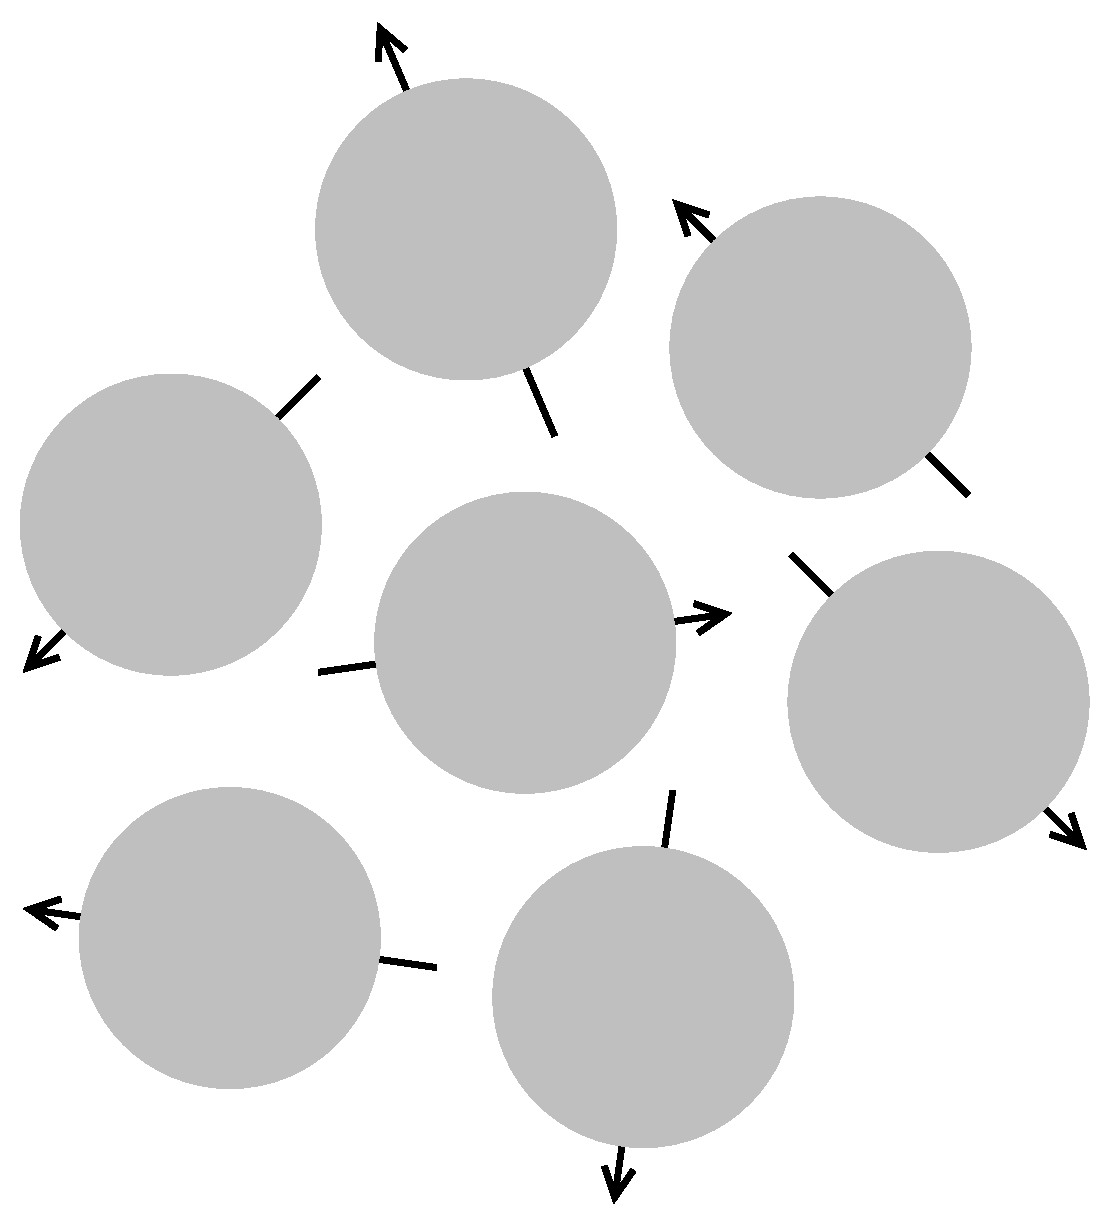
\includegraphics[height=25mm]{eps/chapitre1/Spin_Repos.eps}\label{fig:intro:mag:repos}}
\hspace{2mm}
\subfigure[]{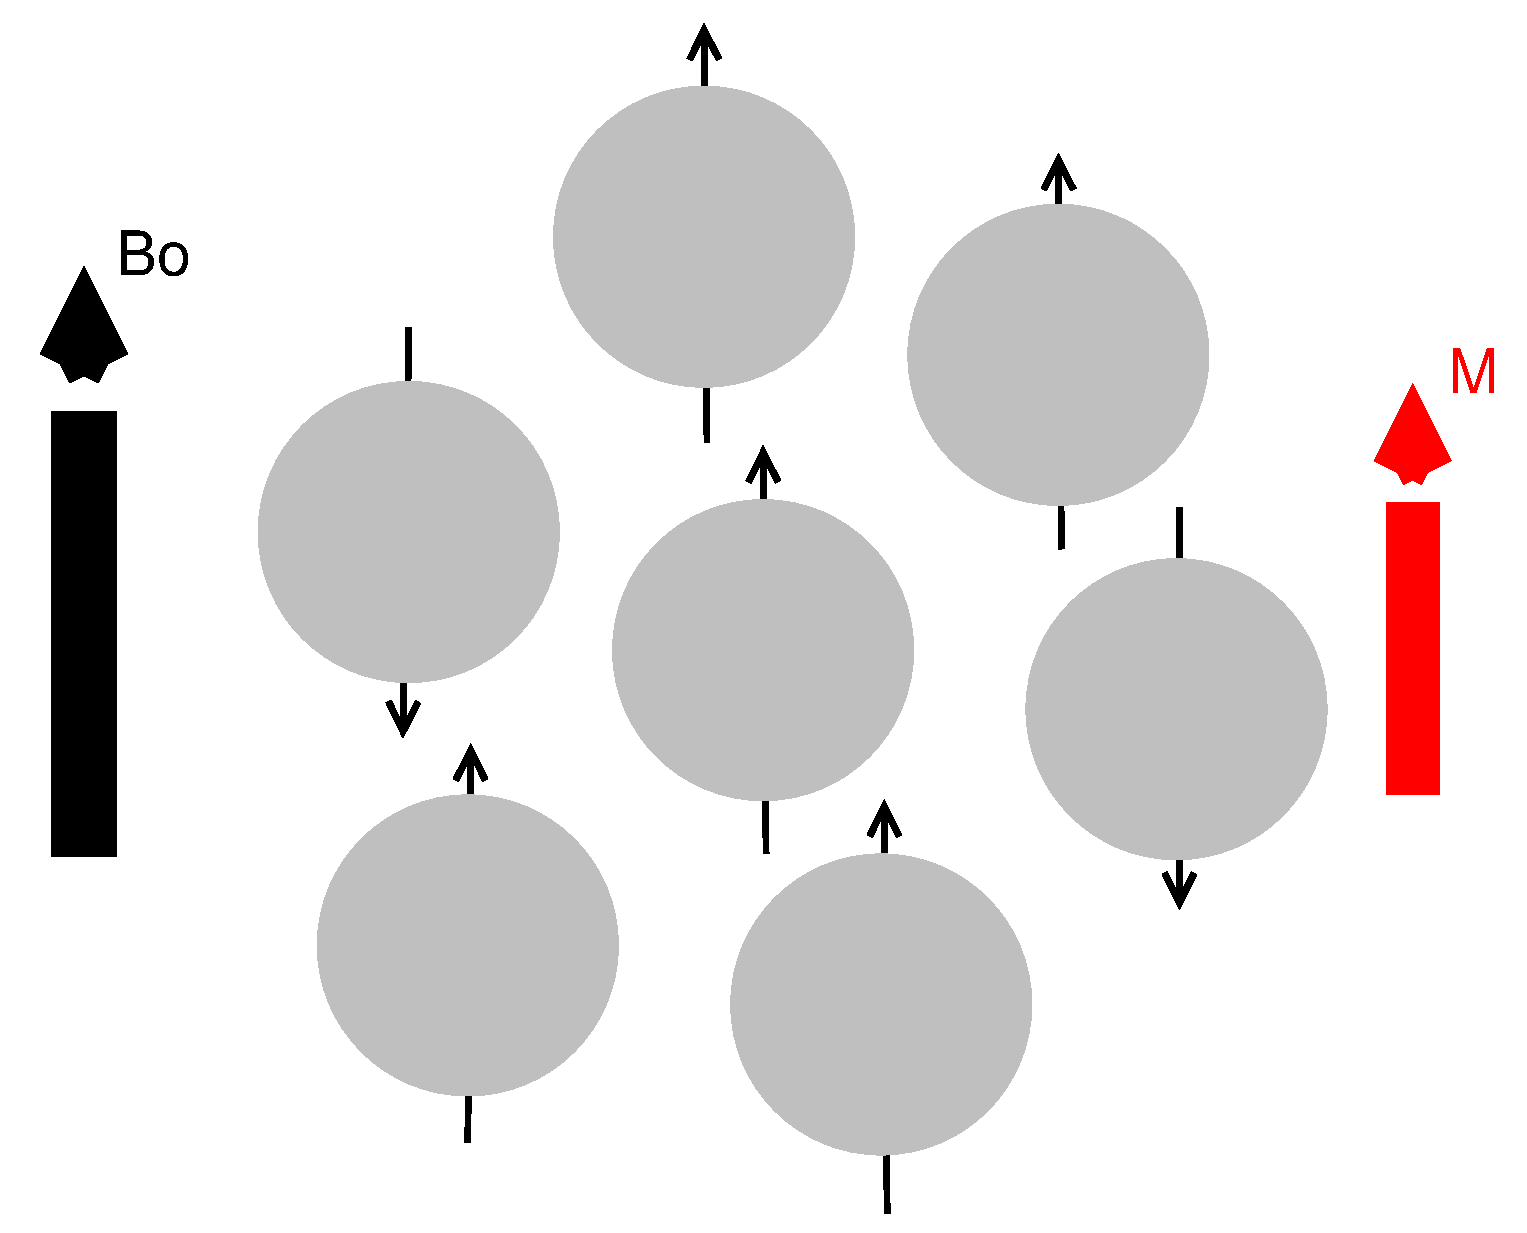
\includegraphics[height=25mm]{eps/chapitre1/Spin_Equilibre.eps}\label{fig:intro:mag:equilibre}}\\
% \hspace{2mm}
\subfigure[]{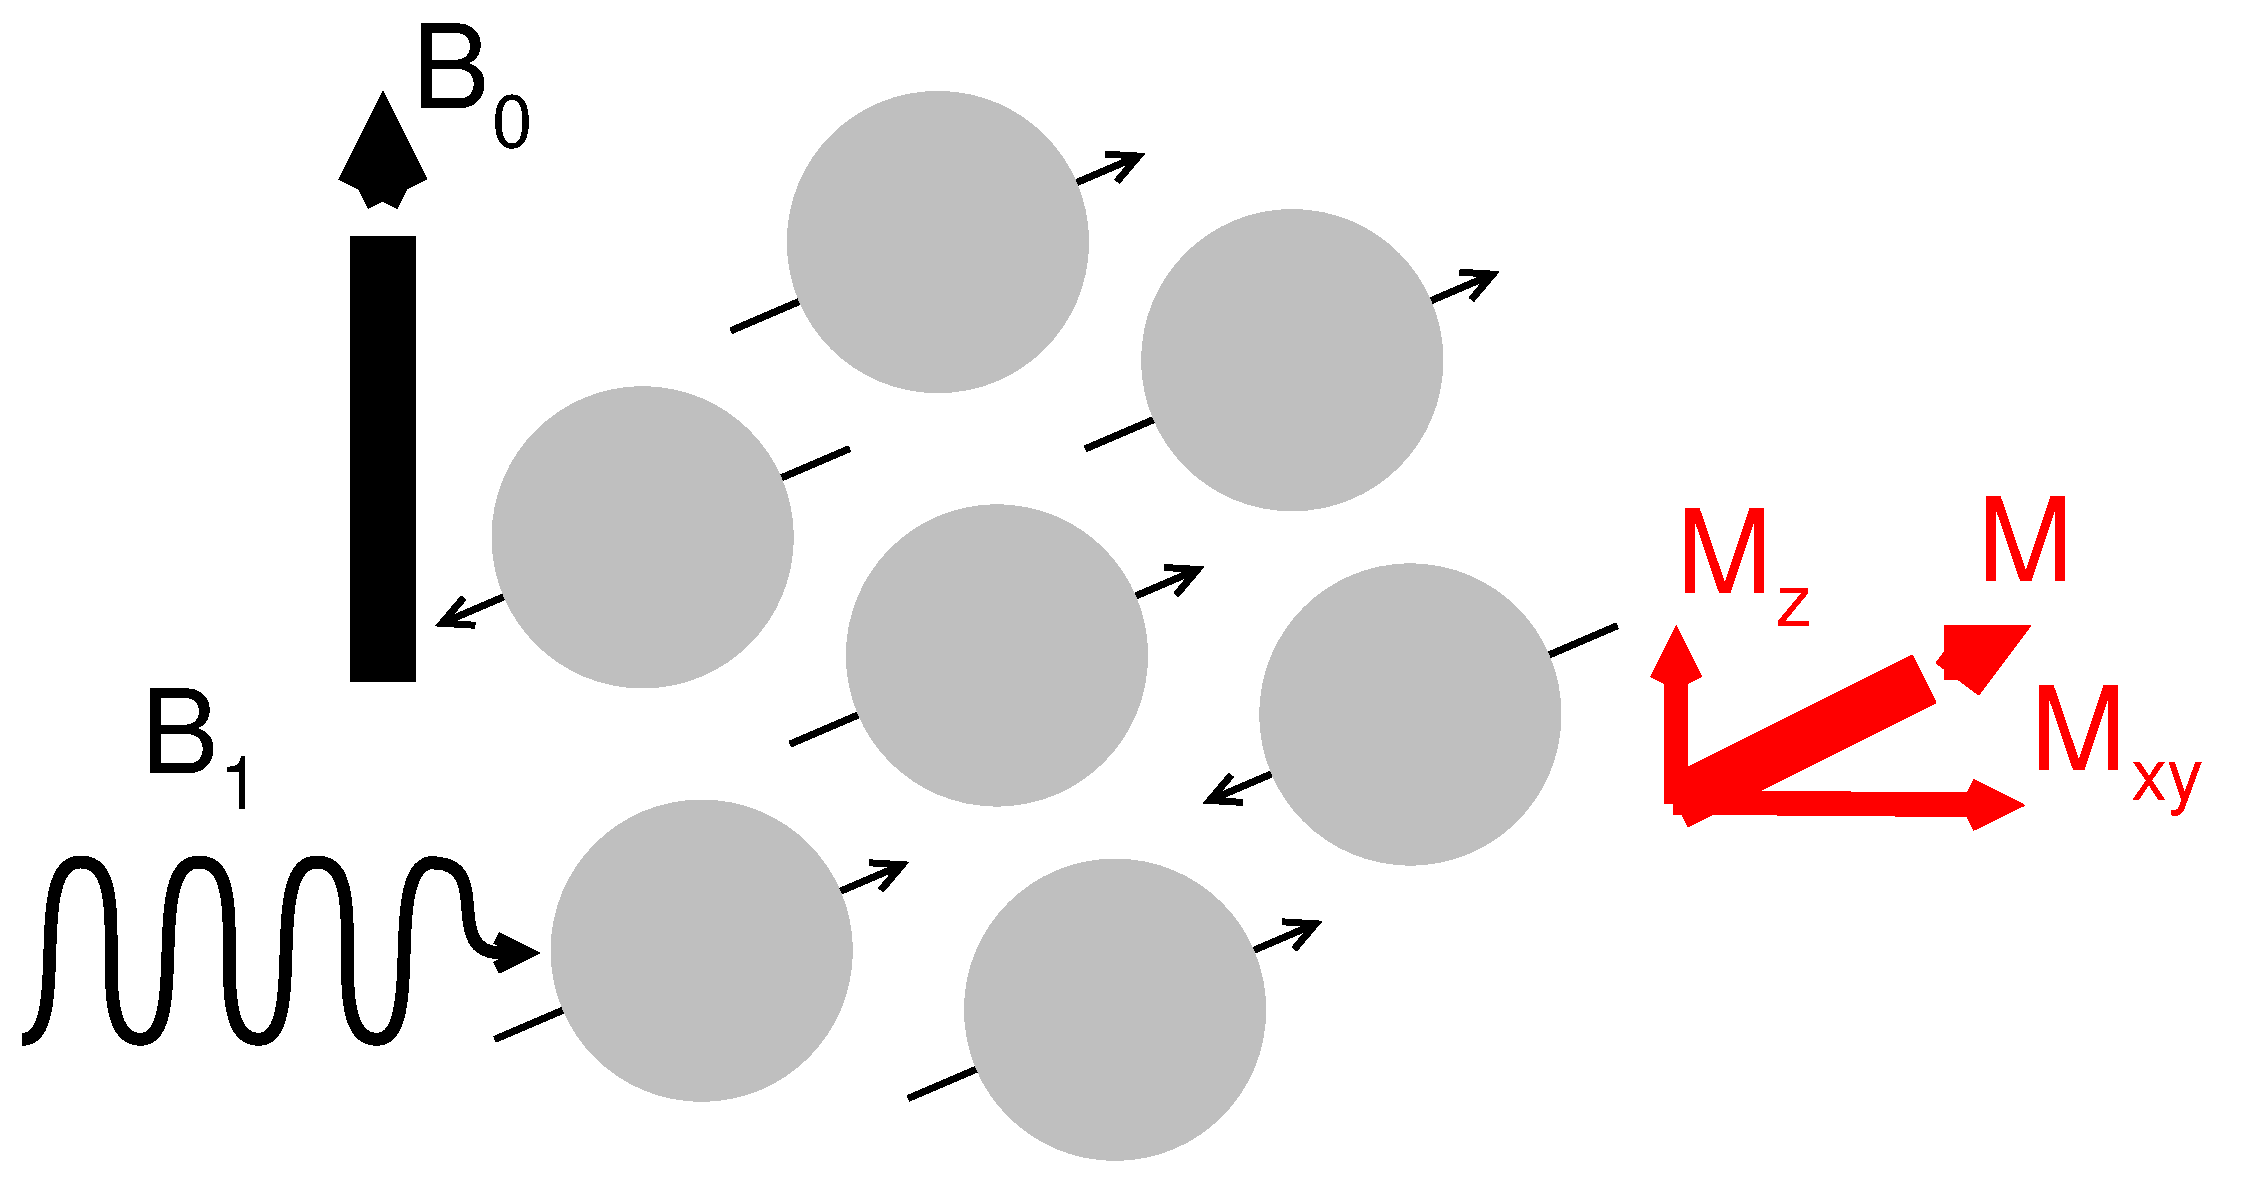
\includegraphics[height=25mm]{eps/chapitre1/Spin_Excitation.eps}\label{fig:intro:mag:excitation}}
\hspace{2mm}
\subfigure[]{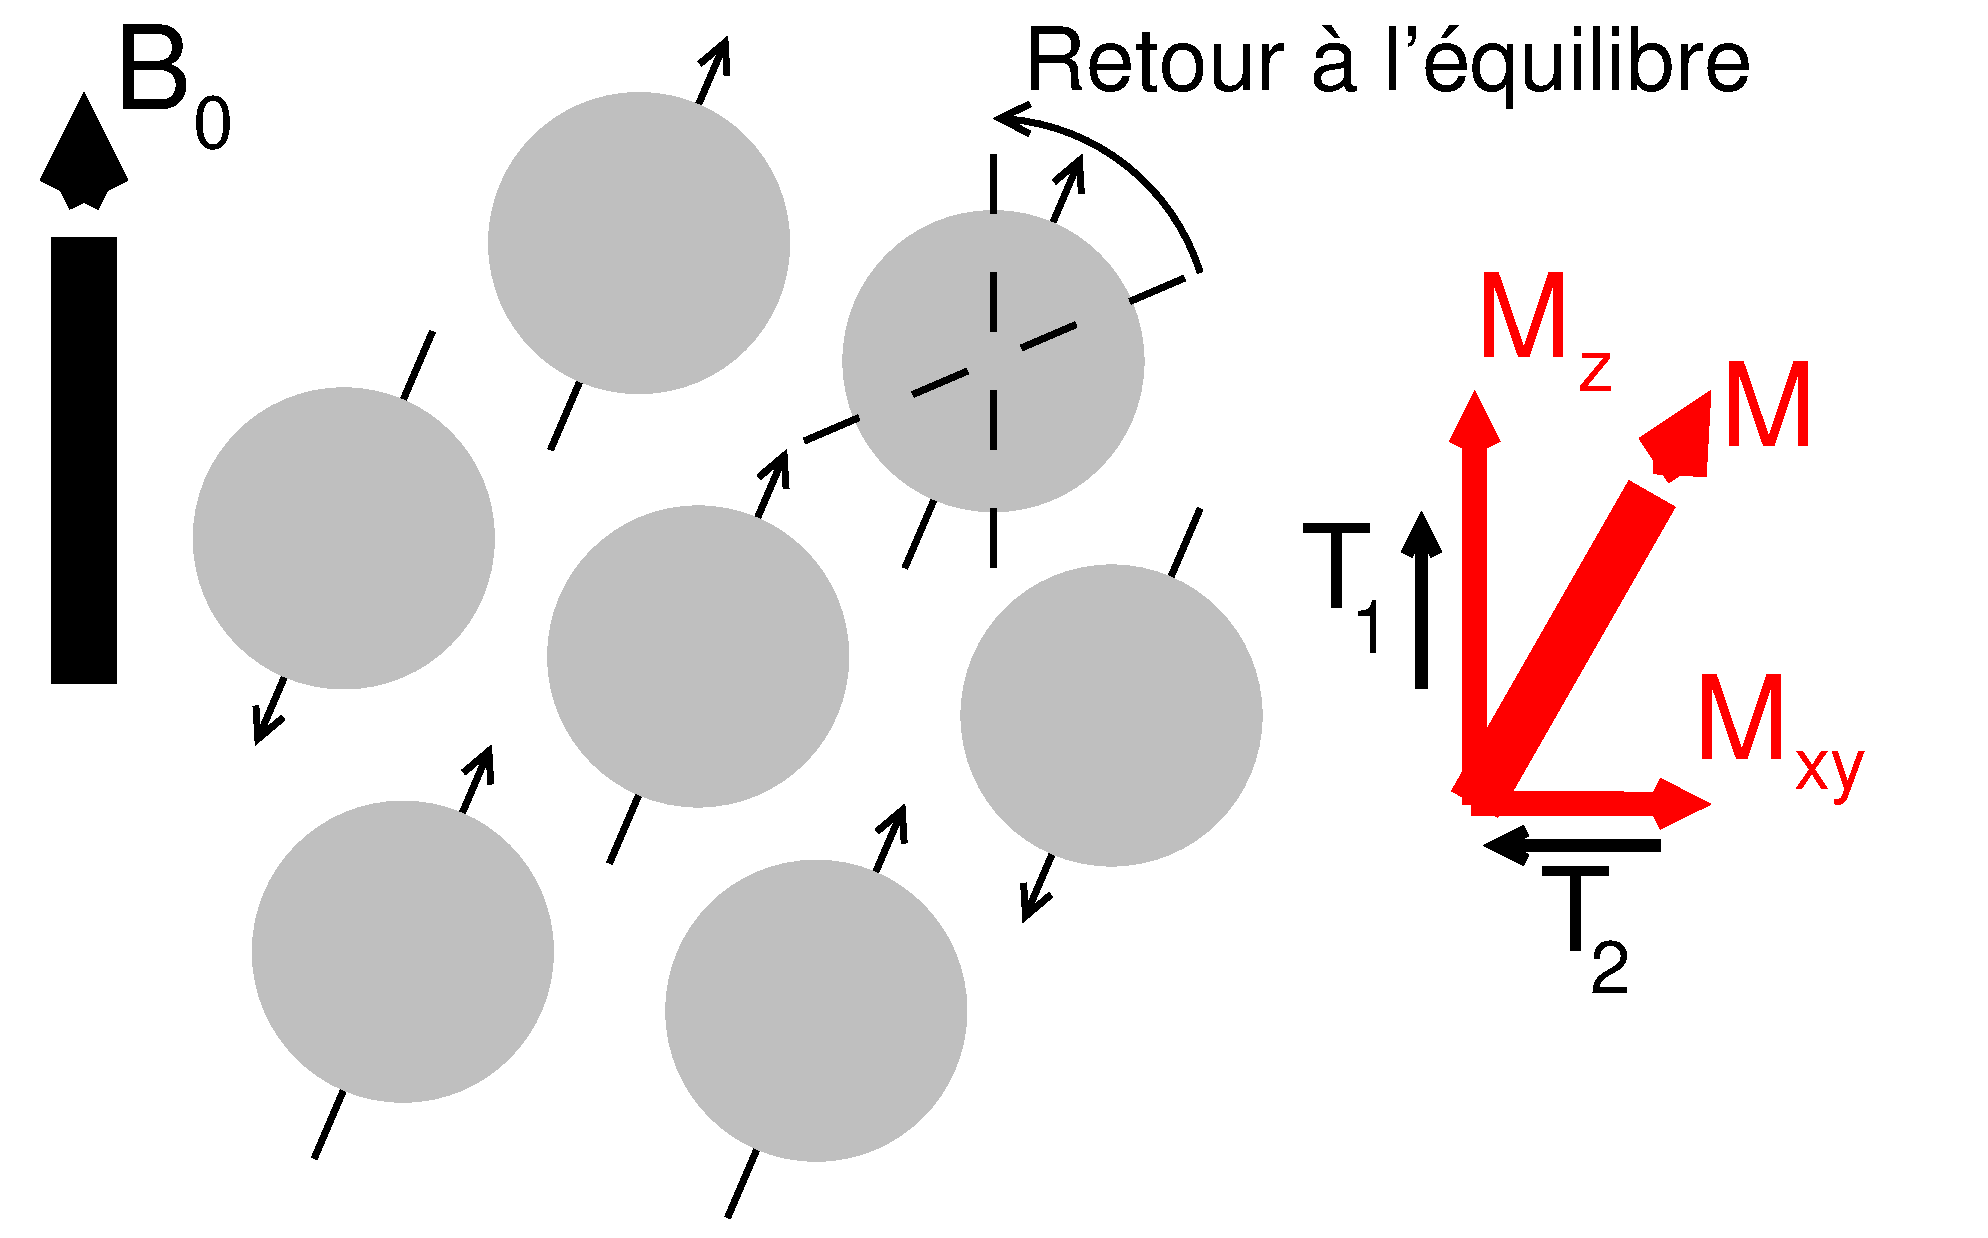
\includegraphics[height=25mm]{eps/chapitre1/Spin_Relaxation.eps}\label{fig:intro:mag:relaxation}}
\hspace{-5mm}
\caption[Principe de la RMN]{\emph{Principe de la RMN. (a) Etat initial : r�sultante $M$ nulle. (b) Etat d'�quilibre : orientation des spins selon $B_0$. (c) Phase d'excitation : �mission d'un signal RF et apparition d'un composante transversale $M_{xy}$. (d) Phase de relaxation : disparition de la composante $M_{xy}$ selon la constante caract�ristique $T_2$ et croissance de la composante $M_z$ selon la constante caract�ristique $T_1$.}}
\label{fig:intro:mag}
\end{center}
\end{figure}

Le ph�nom�ne de la RMN repose sur les propri�t�s magn�tiques des noyaux des atomes.
En effet, un atome ayant un nombre impair de protons poss�de un moment magn�tique, appel� \emph{spin} nucl�aire.
En l'absence de tout champ magn�tique ext�rieur, l'ensemble de ces \emph{spins} est orient� de mani�re al�atoire, conduisant � une r�sultante magn�tique nulle (voir Figure~\ref{fig:intro:mag:repos}).

La premi�re �tape pour observer le ph�nom�ne de RMN est de placer l'ensemble des atomes dans un champ magn�tique constant $B_0$ (d�finissant ainsi la direction $z$ de l'espace).
L'ensemble des \emph{spins} s'orientent alors suivant la direction de $B_0$ selon deux orientations : l'une dans le sens de $B_0$ (parall�le) et l'autre dans le sens inverse (anti-parall�le) (voir Figure~\ref{fig:intro:mag:equilibre}).
Statistiquement, le nombre de \emph{spins} orient�s dans le sens de $B_0$ �tant plus nombreux, la r�sultante magn�tique $M$ devient non nulle est parall�le � $B_0$.
Les \emph{spins} atteignent alors un �tat d'�quilibre �nerg�tique et adopte un mouvement de pr�cession autour de $B_0$ dont la vitesse est proportionnelle � l'intensit� de $B_0$ et qui est caract�ris�e par la fr�quence angulaire : $\omega_0 = \gamma B_0$ (fr�quence de Larmor), $\gamma$ repr�sentant le rapport giromagn�tique de l'atome consid�r�.

La deuxi�me �tape est l'excitation du syst�me par un champ magn�tique $B_1$ orient� perpendiculairement � $B_0$ (soit dans le plan $xy$) (voir Figure~\ref{fig:intro:mag:excitation}).
Ce champ magn�tique se pr�sente sous la forme d'ondes radio-fr�quences (RF) ayant la m�me fr�quence que la fr�quence de Larmor des atomes consid�r�s.
Les atomes entrent alors en r�sonance, ce qui se manifeste au niveau quantique par une absorption d'�nergie.
L'aimantation globale $M$ bascule alors dans la direction de $B_1$, ce qui se traduit par une diminution de la composante longitudinale $M_z$ (parall�le � $B_0$) et par l'apparition d'une composante transversale $M_{xy}$.

La troisi�me �tape est la relaxation (voir Figure~\ref{fig:intro:mag:relaxation}). 
Une fois le signal RF interrompu, le syst�me restitue l'�nergie absorb�e pour revenir � l'�tat d'�quilibre de d�part, entra�nant un r�alignement de l'aimantation $M$ sur $B_0$.
La relaxation longitudinale cro�t exponentiellement selon une constante de relaxation \emph{spin-r�seau} $T_1$ (repr�sentant le temps n�cessaire � la composante $M_z$ pour revenir � $63\mbox{ }\%$ de sa valeur finale).
Elle correspond au transfert de l'�nergie d'un \emph{spin} vers son environnement.
La relaxation transversale d�cro�t exponentiellement selon une constante de relaxation \emph{spin-spin} $T_2$ (repr�sentant le temps n�cessaire � la composante $M_{xy}$ pour revenir � $37\mbox{ }\%$ de sa valeur initiale).
Elle correspond � des transfert d'�nergie entre \emph{spins}.

La derni�re �tape, la lecture du signal, correspond � la captation par des r�cepteurs appropri�s du signal RF �mis lors de la restitution d'�nergie (appel�s signaux de pr�cession libre).
C'est ce signal qui doit �tre trait� apr�s transform�e de Fourier, selon sa fr�quence, son amplitude et sa dur�e, qui sont caract�ristiques de l'�volution de l'aimantation $M$.
% Principe de la RMN : deux articles ind�pendant qui sont \cite{Bloch:PhyRev:1946} et \cite{Purcell:PhyRev:1946}.


\subsection{Formation des images et contrastes}

\subsubsection{Le cas g�n�ral}

Les applications m�dicales courantes se basent sur l'excitation du proton d'hydrog�ne des mol�cules d'eau pr�sents en grande quantit� dans le corps humain.
L'obtention d'une image en 2D ou 3D gr�ce � l'IRM se fait en diff�renciant les diff�rentes parties d'une zone consid�r�e gr�ce � des gradients directionnels appliqu�s dans les trois directions de l'espace par des bobines de gradients.
Tout d'abord, un gradient de coupe (dans la direction de $z$) est appliqu� afin de s�lectionner la coupe que l'on cherche � acqu�rir.
Puis, les gradients de d�calage de phase et de fr�quence sont appliqu�s de mani�re � s�lectionner la ligne et la colonne de la matrice dont on cherche � acqu�rir le signal.
Une fois la matrice remplie, une transform�e de Fourier inverse permet de reconstruire une image en passant du domaine fr�quentiel au domaine spatial.

Diff�rents types de contrastes peuvent �tre appliqu�es � l'image selon l'information que l'on cherche � mettre en valeur, donnant ainsi plusieurs modalit�s d'image (T1, T2 ou densit� de protons).
Ces diff�rentes modalit�s sont obtenues en jouant sur les param�tres d'acquisition de l'IRM, qui sont : le temps de r�p�tition (TR) (temps entre deux impulsions RF cons�cutives) et le temps d'�cho (TE) (temps s�parant l'impulsion RF et l'acquisition du signal).
Un TR court et un TE court permettent d'obtenir une image pond�r�e en T1, un TR et un TE long permettent d'obtenir une image pond�r�e en T2, tandis qu'un TR long et un TE court entra�nent la formation d'une image pond�r�e en densit� de protons.

Diff�rentes s�quences ont �t� d�finis afin d'obtenir une image � partir de l'IRM.
Ces s�quences repr�sentent diff�rentes combinaisons d'ondes RF et d'impulsions de gradients.
Chacune d'entre elles pr�sente ses avantages et ses inconv�nients en terme de temps d'acquisition et d'introduction d'artefacts (par exemple hypersignal des graisses, baisse du rapport signal � bruit, \ldots{}).

\subsubsection{Le cas sp�cifique des f\oe tus}

Dans le cadre de l'imagerie du f\oe tus, il a �t� mis en �vidence que les temps d'acquisition des IRM (spin-�cho ou fast-spin-�cho) �taient beaucoup trop longs et donc beaucoup trop sensibles aux mouvements des sujets.
Cependant, des s�quences reposant sur des �cho de spin ultra-rapides ont �t� d�velopp�es et plusieurs publications montrent leur utilit� dans le cadre de l'imagerie c�r�brale f\oe tale \cite{Yamashita:AJR:1997, Hubbard:SemPer:1999, Glenn:AJNR:2006}.
Ces s�quences permettant d'acqu�rir une coupe en moins d'une seconde, elles permettent d'apporter une r�ponse aux mouvements du f\oe tus et � la respiration de la m�re qui risquent de parasiter l'acquisition.
Cependant, les techniques d'acquisition 3D ne sont pas encore suffisamment performantes~\cite{Studholme:ARBE:2010}, conduisant � r�aliser des acquisitions sous formes de piles de coupes 2D (l'�paisseur d'une coupe �tant en g�n�ral d'environ $3\mbox{ }mm$).
L'�paisseur de coupes (n�cessaire pour procurer une bonne r�solution � la coupe acquise ainsi que pour b�n�ficier d'un bon rapport signal � bruit) emp�che cependant de r�aliser une r�elle analyse 3D du cerveau.
De plus, l'acquisition sous formes de piles 2D ne garantit pas une coh�rence anatomique entre les coupes.
Trois s�ries d'acquisitions sont alors r�alis�es (dans les directions axiales, sagittales et coronales), de mani�re � obtenir une vision compl�mentaire du volume c�r�brale du cas �tudi�.

Malgr� ces d�fauts, l'IRM c�r�brale de f\oe tus s'est r�v�l�e comme un outil important dans certains cas cliniques.
Elle a notamment �t� utilis�e pour r�aliser des �tude de population \cite{Grossman:NeuroImage:2006}, �valuer l'hypertrophie des ventricules \cite{Kazan-Tannus:AJR:2007}, identifier des malformations c�r�brales \cite{Rolo:ArcPedObs:2011} ou encore pour identifier des infections \cite{Barkovich:ChildNervousSys:2003}.
% Livre en ligne : \cite{Hornak:Online:1996}.

% Comment obtient-on une image T1, T2 ou densit� de protons.
% \cite{Yamashita:AJR:1997} : article mettant en �vidence les avantages de l'ultra-fast spin echo dans le cadre de l'imagerie f�tale.
% \cite{Hubbard:SemPer:1999} : article d�crivant le protocole d'IRM pour les foetus


\subsection{Caract�ristiques}
\label{intro:irm:carac}

Cette section d�crit les diff�rents artefacts rencontr�s lors de l'exploitation des images issus d'une IRM.
Ils peuvent cependant �tre corrig� en post-traitement et la connaissance de leur origine permet de mieux les appr�hender.

\subsubsection{Le bruit}

L'IRM �tant un dispositif de mesure physique, le signal capt� est entach� de bruit provenant aussi bien du patient (agitation thermique des protons � l'origine d'�missions parasites) que de la cha�ne de mesure (bruit \og{} �lectronique \fg).
Le rapport signal � bruit (SNR) caract�rise l'amplitude du bruit par rapport � l'amplitude du signal.
De mani�re g�n�rale, le bruit pr�sent dans les IRM suit une distribution de Rice \cite{Sijbers:TMI:1998}, qui peut cependant �tre approxim� par une distribution gaussienne dans les zones o� l'intensit� n'est pas proche de z�ro et avec un SNR sup�rieur � $3$.
Cette approximation est valide dans la mati�re grise, la mati�re blanche et dans une moindre mesure dans le LCR.
% \cite{Sijbers:TMI:1998} : article pr�cisant que le bruit rencontr� dans les IRM est de type ricien et peut �tre approxim� par une distribution gaussienne avec un haut SNR.

\subsubsection{Le volume partiel}

Du fait de la discr�tisation de l'espace, plusieurs objets peuvent se retrouver dans un m�me voxel.
Les signaux issus de ces objets se m�langent alors, contribuant � fournir un signal interm�diaire pour le voxel consid�r�.
En IRM, cet effet se manifeste surtout � la fronti�re entre les tissus (LCR - mati�re grise, mati�re grise - mati�re blanche, \ldots{}) ou lorsque certaines structures sont beaucoup trop fine pour �tre prise en compte par l'imageur (petits vaisseaux sanguins, ramification du cortex, \ldots{}).

\begin{figure}[!t]
\begin{center}
\subfigure[]{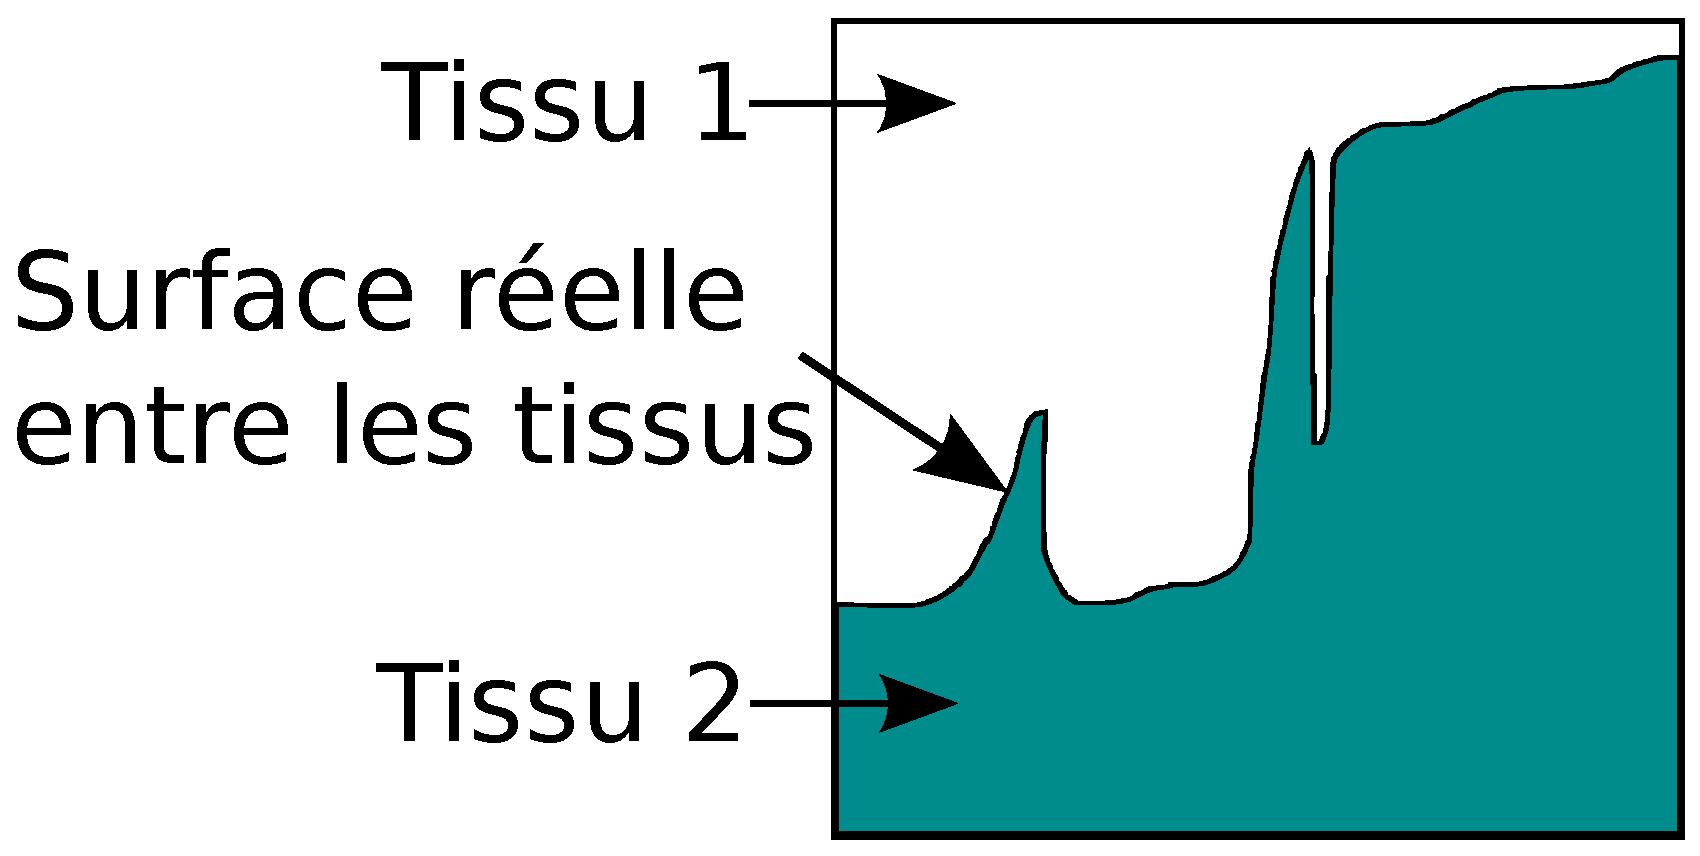
\includegraphics[height=25mm]{eps/chapitre1/Vol_Partiel_True.eps}}
\hspace{2mm}
\subfigure[]{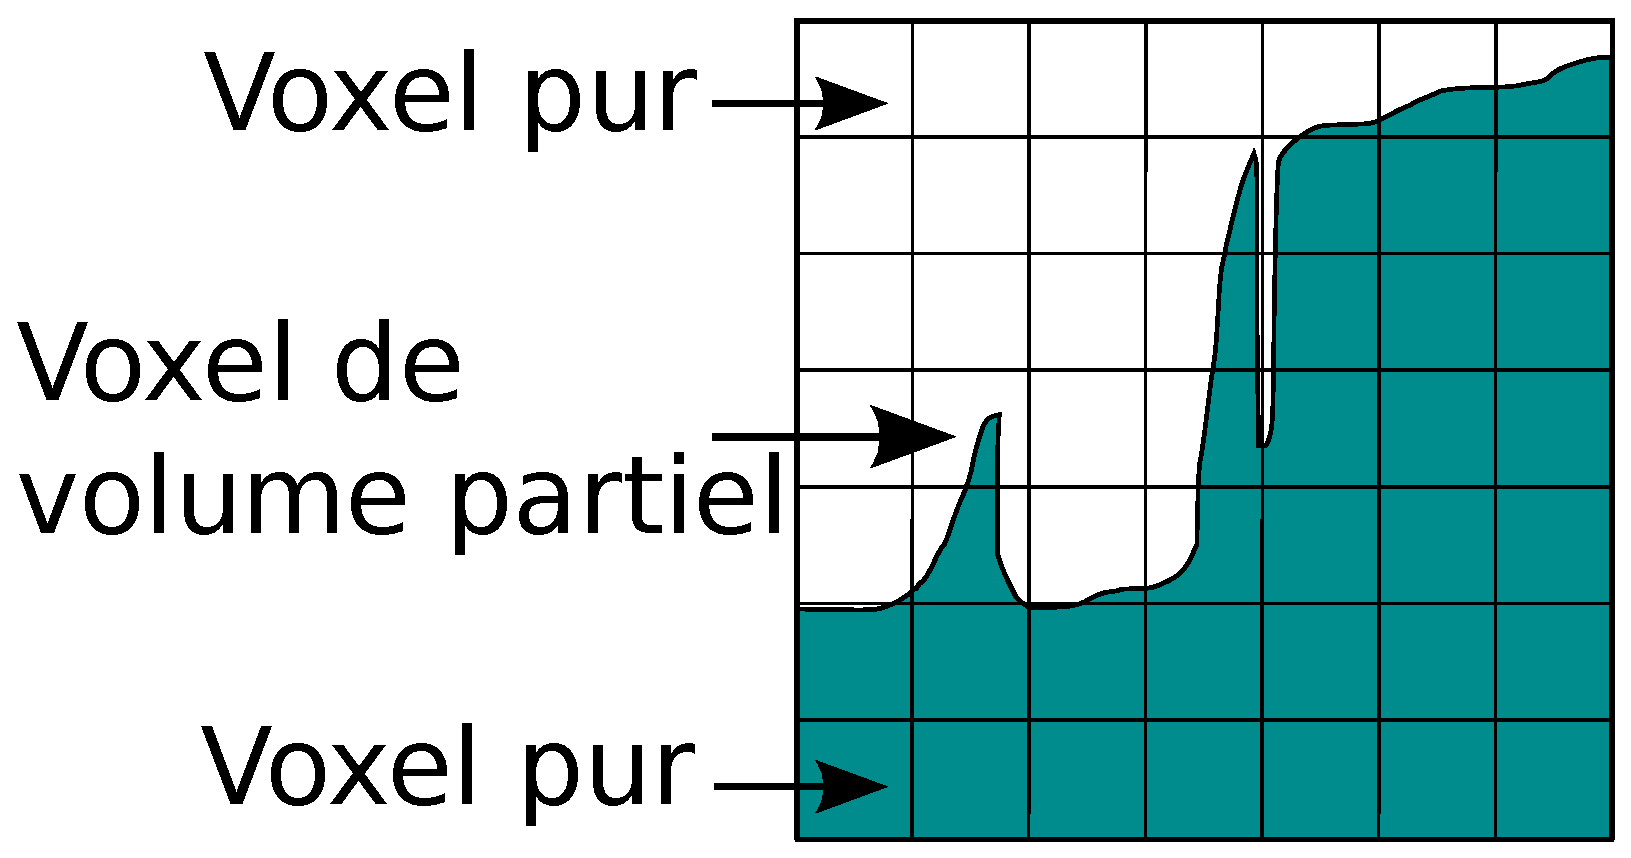
\includegraphics[height=25mm]{eps/chapitre1/Vol_Partiel_Discretisation.eps}}
\hspace{2mm}
\subfigure[]{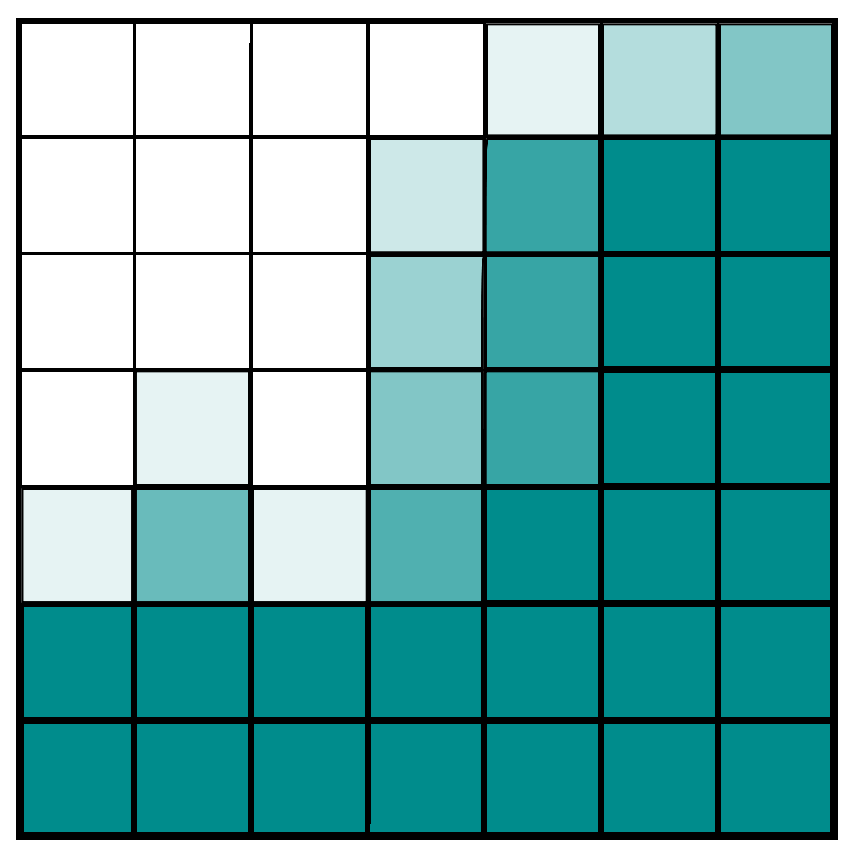
\includegraphics[height=25mm]{eps/chapitre1/Vol_Partiel_Final.eps}}
\caption[Volume Partiel en IRM]{\emph{Volume partiel en IRM}}
\label{fig:nlm:kernels}
\end{center}
\end{figure}


\subsubsection{Le biais en intensit�}

Cet artefact se manifeste par une h�t�rog�n�it� en intensit� pour un m�me tissu c�r�bral.
Elle s'explique par l'inhomog�n�it� des champs $B_0$ et $B_1$, la qualit� de l'antenne de r�ception, ou encore par une composition histologique diff�rente d'un m�me tissu en fonction de sa localisation.
Les effets de susceptibilit� magn�tique jouent �galement un r�le dans la formation de l'inhomog�n�it� en intensit�.

Ce biais repr�sente une difficult� pour toute m�thode de classification des voxels reposant sur leur intensit� et supposant que l'intensit� d'une classe est constante sur l'ensemble de l'image.
La plupart de ces m�thodes soit, l'�limine par un pr�-traitement, soit le prennent directement en compte dans la classification.

\subsubsection{Autres}

% Nous pouvons encore signaler plusieurs types d'artefacts.
Les artefacts de mouvement (pouvant �tre tr�s probl�matique dans le cas de l'IRM f\oe tale) sont dus aux mouvements du patient pendant l'examen, ainsi qu'aux mouvements physiologiques (respiration, flux sanguin).
L'impact de ces artefacts est variable selon le moment de l'acquisition mais il se traduit g�n�ralement par l'apparition d'images fant�mes de la structure en mouvement.
Ceci est particuli�rement sensible en IRM f\oe tale ou l'on doit tenir compte non seulement des mouvements du f\oe tus (si il n'est pas s�dat�), mais �galement de la respiration de la m�re (c'est pourquoi certains protocoles d'acquisition pr�voient une apn�e de la m�re pendant l'acquisition proprement dite).

Diff�rentes techniques permettent de r�duire l'influence de ces artefacts (par exemple : l'introduction de bobines de shim pour assurer l'homog�n�it� du champs $B_0$).
Cependant, l'image finale sera toujours perturb�e par un certain nombre d'entre eux, et les m�thode de classification des �l�ments de l'image doivent en tenir compte.

%------------------------------------------------------------------------Anatomie et maturation c�r�brale----------------------------------------------------------------------------------------

\section{Anatomie et maturation c�r�brale}

Cette section pr�sente succinctement quelques notions fondamentales d'anatomie c�r�brale.
Nous pr�sentons tout d'abord les tissus c�r�braux chez l'adulte, puis nous nous int�resserons au cas des f\oe tus.
Cette derni�re partie d�crira l'�volution du cerveau au cours de la grossesse.

\subsection{Les diff�rents tissus c�r�braux}

\begin{figure}[!t]
\begin{center}
\subfigure[]{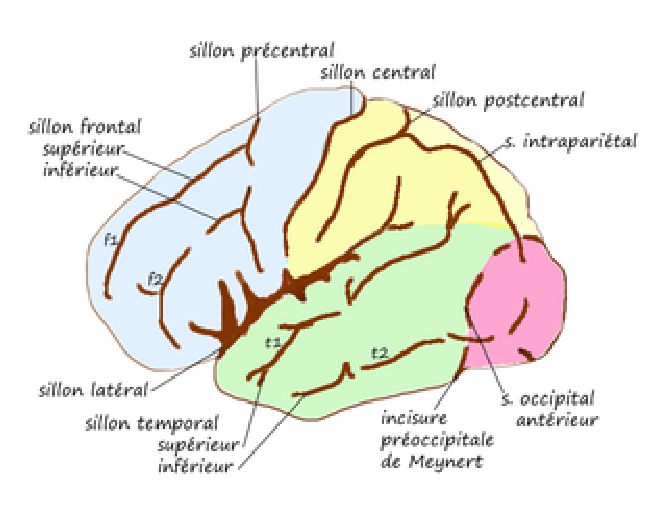
\includegraphics[height=55mm]{eps/chapitre1/Sillons_externe.eps}}
\subfigure[]{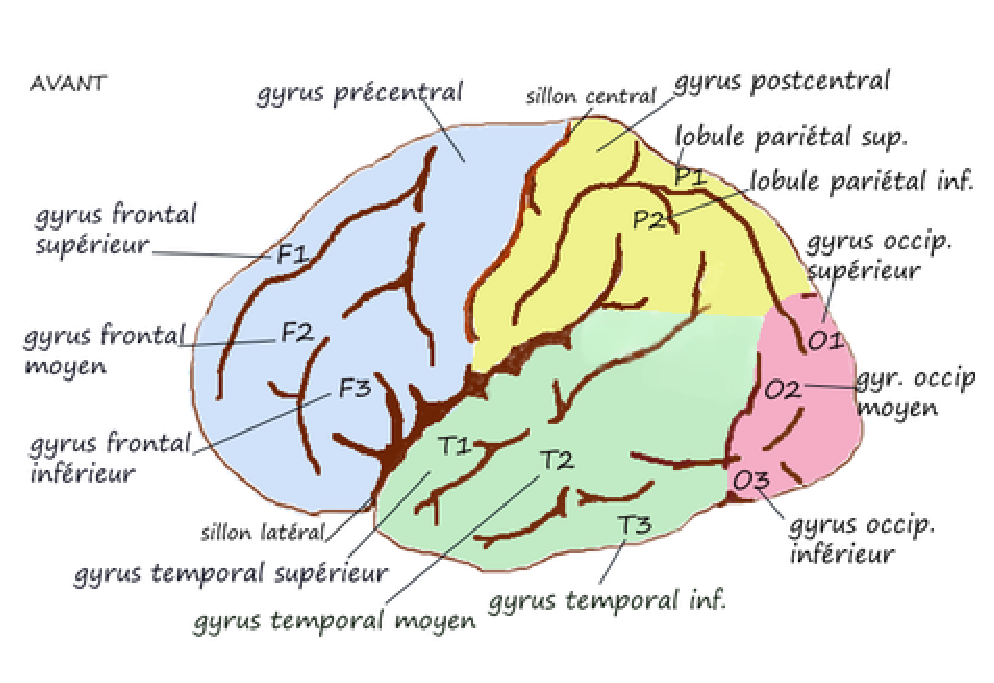
\includegraphics[height=55mm]{eps/chapitre1/Gyrus_externe.eps}}
\hspace{-5mm}
\caption[Sillons et gyri c�r�braux]{\emph{Principaux sillons (a) et gyri (b) c�r�braux d'un cerveau adulte. L�gende : lobe frontale (bleu), lobe pari�tal (jaune), lobe temporal (vert), lobe occipital (rouge) (images issues de : \url{fr.wikipedia.org}).}}
\label{Intro:Brain:Adult}
\end{center}
\end{figure}

L'enc�phale est constitu� du cerveau, du cervelet et du tronc c�r�bral.
Le cerveau lui-m�me est compos� de trois mati�re principales que sont : la mati�re grise (MG), la mati�re blanche (MB) et le liquide c�phalo-rachidien (LCR).
Le LCR se situe tout autour du cerveau et remplit le syst�me ventriculaire.
Il permet d'amortir les chocs et les mouvements qui pourraient endommager le cerveau.
La mati�re blanche est constitu�e des axones my�linis�e des neurones, permettant la transmission de l'information � travers le cerveau.
La mati�re grise est compos�e essentiellement des corps cellulaires et des dendrites des neurones ainsi que des cellules gliales.
Cette mati�re grise est r�partie dans deux grandes structures diff�rentes : les noyaux et le cortex.

Le cortex en lui m�me est une couche de cellules de 1 � 4.5 mm d'�paisseur~\cite{Fischl:PNAS:2000}.
Il est pliss� par diff�rents sillons formant les circonvolution c�r�brales, ou \emph{gyri}.
Les scissure les plus profondes d�limitent plusieurs aires appel�s des lobes (voir Figure~\ref{Intro:Brain:Adult}). 
Les quatre grands lobes du cerveau sont les lobes : frontal, pari�tal, temporal et occipital.

Les sillons principaux du lobe frontal sont : le sillon pr�central et les sillons frontaux inf�rieurs et sup�rieurs.
Ceux du lobe temporal sont : les sillons temporals inf�rieurs et sup�rieurs.
Ceux du lobe pari�tal sont : le sillon postcentral et le sillons intrapari�tal.

Le sillon central marque la fronti�re entre les lobes frontal et pari�tal et le sillon lat�ral celle entre les lobes frontal et temporal.
Le repli de l'\emph{insula} est compl�tement recouvert par les lobes frontal et temporal.
Ces sillons sont importants � noter car leur apparition au cours de la grossesse permet de d�terminer le degr� de maturit� du cerveau �tudi�~\cite{Levine:Radiology:1999}.

\subsection{Maturation c�r�brale}

\subsubsection{La mise en place du syst�me nerveux}

\begin{figure}[!t]
\begin{center}
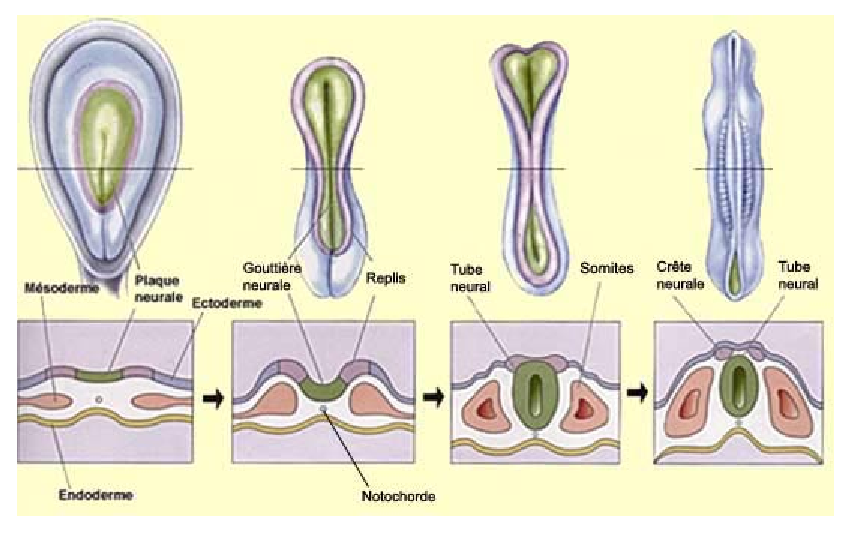
\includegraphics[height=100mm]{eps/chapitre1/Tube_Neural.eps}
\hspace{-5mm}
\caption[Formation du tube neural]{\emph{Formation du tube neural � l'origine du syst�me nerveux (image issue de : \url{http://lecerveau.mcgill.ca})}}
\label{fig:intro:tube}
\end{center}
\end{figure}

La formation du syst�me nerveux commence tr�s t�t au cours de la grossesse, c'est � dire d�s la troisi�me semaine.
A ce stade, la gastrulation de l'embryon (r�organisation des cellules apr�s la nidation dans l'ut�rus) a d�j� eu lieu et le syst�me nerveux se pr�sente sous la forme d'une couche aplatie de cellules appel�e la plaque neurale.
Cette plaque va tout d'abord s'invaginer, formant ainsi la goutti�re neurale (voir Figure~\ref{fig:intro:tube}).
La fermeture de cette goutti�re, tout d'abord par son milieu, puis dans sa partie ant�rieure et post�rieure, constitue alors le tube neural dont la partie dorsale, la cr�te neurale, est � l'origine du syst�me nerveux p�riph�rique.
A la fin de la quatri�me semaine de grossesse, ce processus est achev� et deux processus vont avoir lieux en parall�le : l'histogen�se, c'est � dire la diff�renciation cellulaire � partir des cellules souches, et la formation des grandes r�gions du cerveau. 

\begin{figure}[!t]
\begin{center}
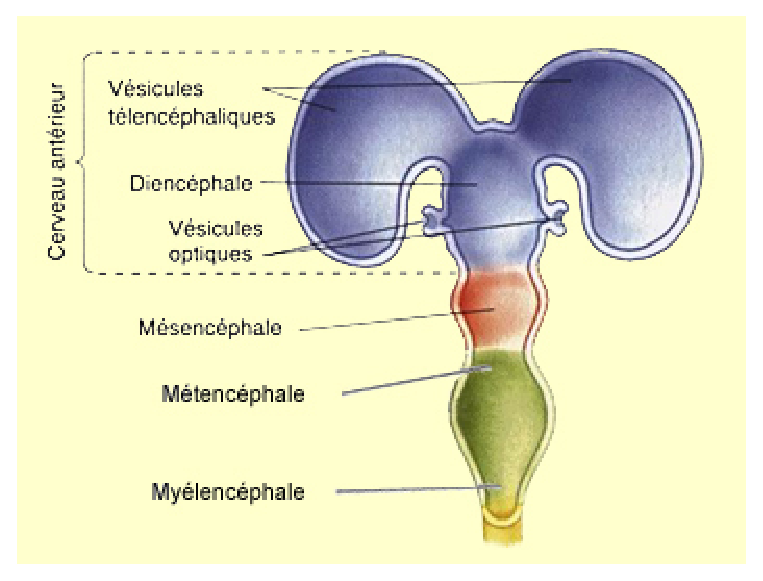
\includegraphics[height=100mm]{eps/chapitre1/vesicules.eps}
\hspace{-5mm}
\caption[Formation des grandes r�gions du cerveau]{\emph{Formation des grandes r�gions du cerveau (image issue de : \url{http://lecerveau.mcgill.ca})}}
\label{fig:intro:vesicules}
\end{center}
\end{figure}

L'enc�phale se constitue par subdivision de la partie ant�rieure du tube neural en trois v�sicules primaires (prosenc�phale, m�senc�phale et rhombenc�phale) puis en cinq v�sicules secondaires (t�lenc�phale, dienc�phale, m�senc�phale, m�tenc�phale et my�lenc�phale) (voir Figure~\ref{fig:intro:vesicules}).
Le t�lenc�phale est constitu� de deux gros v�sicules qui deviendront les h�misph�res c�r�braux.
Le dienc�phale comprends les �l�ments qui formeront le thalamus, l'hypothalamus, l'hypophyse, la glande pin�ale et la r�tine.
Le m�senc�phale est le seul v�sicule primaire qui ne se divise pas.
Son �volution est plus lente et aboutit entre autres � la formation du tegmentum (r�gion responsable par exemple du maintien de la posture) et des colliculi sup�rieurs et inf�rieurs (responsables des transmissions visuelles et auditives).
Le m�tanc�phale donnera jour au cervelet (entre autres) et le my�lanc�phale deviendra le bulbe rachidien.
Le reste du tube neural formera la moelle �pini�re par �paississement des parois, conduisant � une r�duction du diam�tre du tube jusqu'� aboutir au canal spinal.

A partir de la huiti�me semaine, le d�veloppement c�r�bral en temps que tel commence tout d'abord par la multiplication des neurones et des cellules gliales dans les zones germinales autour des ventricules.
Puis, l'ensemble des neurones va migrer le long de cellules gliales radiales pour former les diff�rentes couches du cortex.
Cette migration se poursuit jusqu'� 20 semaines et peut s'�tendre jusqu'� 24 semaines.


\subsubsection{L'�volution du cortex c�r�bral}

Cette partie est issue de plusieurs �tudes anatomiques (par exemple celle de \cite{Chi:AnnNeuro:1977}), qui ont �tudi�es plusieurs centaines de cas de mani�re � d�gager un sch�ma de d�veloppement global du cortex humain et ont �tablit quelques propri�t� int�ressante comme l'assym�trie du lobe temporal gauche � 31 semaines (plus riche en sillons secondaires et tertiaires) (observation semblant indiquer la dominance de l'h�misph�re gauche dans la gestion du langage et de la parole~\cite{Chi:ArNeuro:1977}).
L'�tude de ce d�veloppement est tr�s importante car l'observation de l'�tat du cortex \emph{in utero} par un imageur IRM est un bon indicateur de la maturation c�r�brale d'un patient \cite{Levine:Radiology:1999}.

Tr�s rapidement, les premi�res fissures c�r�brales apparaissent.
La premi�re d'entre elle est le foss� h�misph�rique, visible � partir de la huiti�me semaine, dont le creusement se fait du c�t� ant�rieur vers le post�rieur et s'ach�ve � la dixi�me semaine de grossesse.
A partir de la quatorzi�me semaine d'am�norrh�e, le sillon lat�ral est visible et est constitu� d'une petite d�pression form�e par le repli de l'insula (partie du cortex repli� profond�ment entre le lobe temporal et le lobe frontal) \cite{Chi:AnnNeuro:1977}.
A partir de la dix-neuvi�me semaine, l'insula est compl�tement form�e.

Le lobe pari�tal est une structure qui reste lisse pendant un long moment � l'exception des sillons central et post-central.
Le premier est une profonde fissure qui appara�t d�s la vingti�me semaine de grossesse avec quelques cas ou il appara�t d�s la dix-septi�me semaine du c�t� droit.
Il commence au niveau de la fosse inter-h�misph�rique et s'�tend vers le bas jusqu'� l'insula pour former une fissure lin�aire au bout de 22 � 23 semaines d'am�norrh�e.
A peu pr�t une semaine s'�coule entre l'apparition du sillon du c�t� droit et du c�t� gauche.
Le sillon post-central suit durant la vingt-cinqui�me semaine.
A partir de la trente-troisi�me semaine, les sillons secondaires sont observables.

La gyration du lobe frontal suit le sch�ma suivant.
Le sillon frontal sup�rieur se forme autour de la vingt-cinqui�me semaine et d�limite le gyrus frontal sup�rieur.
Le sillon frontal inf�rieur peut �tre identifi� � 28 semaines et d�limite les gyri frontaux m�dian et inf�rieur.
La trente-deuxi�me semaine est caract�ris�e par l'apparition de sillons secondaires.

Au niveau du lobe temporal, le premier sillon (sillon temporal sup�rieur) appara�t au bout de 23 semaines d'am�norrh�e avec encore une fois un d�calage entre le c�t� droit et le c�t� gauche.
Les sillons temporal m�dians et inf�rieurs sont en g�n�ral visible � la trenti�me semaine.

De mani�re g�n�ral, on observe un d�calage de deux semaines entre la premi�re apparition d'un sillon dans une population et le moment o� il est visible dans 75 � 80\% des cas.
On peut observer que la plupart des sillons et gyri sont observables entre 26 et 28 semaines d'am�norrh�e.
Le dernier trimestre de la grossesse est alors marqu� par un accroissement du volume c�r�bral (le cerveau passe de 60 ml � 160 ml), un approfondissement des sillons d�j� form�s et le d�veloppement de sillons secondaires, voir m�me tertiaires entre 40 et 44 semaines de grossesse.

\subsubsection{L'observation du cortex gr�ce � l'IRM}

Les progr�s r�cents des IRM ont permis de conduire des �tudes anatomiques exhaustives \emph{in vivo}, m�me si quelques travaux ont r�alis� quelques observations (par exemple ceux de~\cite{Girard:AJN:1995} qui ont mis en �vidence quelques variations du signal des images montrant la variation de la densit� cellulaires et les progr�s de la my�linisation).
Plusieurs travaux se sont pench�s sur l'�volution visible du cortex � partir de l'IRM ~\cite{Prayer:PedRad:2006, Glenn:SePer:2009}.
De mani�re g�n�rale, on observe un d�calage entre le moment ou un sillon est observable \emph{ex vivo} et \emph{in vivo}.
Ainsi, le sillon central n'est visible qu'� partir de la vingt-cinqui�me semaine et il faut attendre la vingt-septi�me semaine pour qu'il soit observable dans au moins 75\% des cas.
M�me constat pour le sillon post-central, ou il faut attendre la vingt-huiti�me semaine contre la vingt-cinqui�me \emph{ex vivo}~\cite{Garel:AJNR:2001}.
Les �quipes expliquent ce d�calage par l'�paisseur des coupes et la faible r�solution des IRM, l'effet de volume partiel tendant � masquer de nombreux d�tails anatomiques, surtout sur des structures aussi petites.

N�anmoins, l'ensemble de ces �tude montre que l'IRM est un outil pertinent quant au suivi de la maturation c�r�brale au cours de la grossesse, tout ceci sans danger av�r� pour le f\oe tus.
De plus, cette modalit� peut �tre utilis�e pour r�aliser des �tudes cliniques, telle que celle de \cite{Batchelor} qui � partir d'une segmentation manuelle du cortex a test� diff�rentes mesures de la courbure du cortex en chaque point, de mani�re � suivre plus pr�cis�ment l'�volution des sillons et des gyri.
Cependant, la segmentation manuelle des tissus prend �norm�ment de temps, d'o� la n�cessit� de d�velopper des algorithmes rapides et robustes pour automatiser ce genre de t�che.
\chapter{Segmentation des tissus c�r�braux en IRM : �tat de l'art}
\label{chap:art}
\minitoc

Ce chapitre pr�sente les diff�rentes familles de m�thodes d�velopp�e pour r�pondre � la probl�matique de la segmentation c�r�brale.
La segmentation c�r�brale consiste � trouver les r�gions homog�nes de l'image. 
Ces r�gions sont suppos�es �tre pertinentes, c'est � dire qu'elles doivent mettre en valeur des parties significatives de l'image, telles que les diff�rents tissus c�r�braux (LCR, mati�re grise et mati�re blanche).

Les m�thodes de segmentation doivent prendre en compte les principales caract�ristiques des imageurs par r�sonnance magn�tique (d�crites � la section \ref{intro:irm}) afin de parvenir � un r�sultats pertinents.
Plusieurs familles de m�thodes ont �t� d�velopp�es afin de r�pondre � ce probl�me, sans pour autant repr�senter des cat�gories rigides, de nombreux algorithmes se situant � la fronti�re de ces familles.
Une premi�re section pr�sentera les grandes familles de segmentation class�es selon le principe les r�gissant.
Par la suite, la m�thodologie FCM (\emph{Fuzzy C-Means} ou \emph{C-Moyennes floues}) sera d�taill�e car elle permet une approche tenant compte naturellement du volume partiel pr�sent dans l'image.
Enfin, une derni�re section pr�sentera un �tat de l'art de la segmentation dans le cadre de la maturation c�r�brale.

%------------------------------------------------------------------------Vue d'ensemble----------------------------------------------------------------------------------------

\section{Les diff�rentes familles de segmentation}
\label{sec:overview}

\subsection{Mod�les d�formables}
\label{subsec:snake}

Le principe des mod�les d�formables est l'adaptation d'un contour param�trique � la structure que l'on cherche � segmenter.
Deux types de mod�les d�formables sont distingu�s : les mod�les explicites et les mod�les implicites.

Les mod�les explicites ou \emph{snakes} d�finis par \cite{Kass:IJCV:1988} sont la d�formation it�rative d'un contour param�trique.
Cette d�formation est effectu�e par la minimisation d'une fonctionnelle se pr�sentant comme la somme d'une force externe (le terme d'attache aux donn�e li� au contenu de l'image) et d'une force interne (le terme de r�gularisation prenant en compte l'�lasticit� et la rigidit� du contour).
Les principaux probl�mes des ces mod�les sont leure forte d�pendance � l'initialisation et la difficult� de r�aliser des changements de topologie (fusion ou s�pration de labels). 
En effet, le contour doit �tre d�j� proche de la structure � segmenter et cela reste vrai malgr� l'utilisation des \emph{gradient vector flow} (voir \cite{Xu:TIP:1998}) permettant une moins forte d�pendance � l'initialisation.
Un exemple de leur utilisation est l'article de \cite{McInerney:TMI:1999} qui emploit une formulation particuli�re du contour afin de mieux prendre en compte la complexit� des structures.
Un exemple plus r�cent est l'article de \cite{Colliot:PR:2006}, d�finissant la force externe comme une combinaison du terme d'attache-aux-donn�es et d'une information spatiale concernant la position des diff�rents objets entre eux.
Cette information spatiale se pr�sentent sous la forme de contraintes de localisation (angle et distance) sous forme floue par rapport � une structure de r�f�rence.
Cette m�thodologie a �t� appliqu� � la segmentation des noyaux gris autour des ventricules.

% \cite{Xu:TIP:1998} : snakes et GVF.
% \cite{McInerney:TMI:1999} : Snake avec formulation particuli�re de la surface permettant la segmentation de structures complexes.

Les mod�les implicites sont des m�thodes par ensemble de niveaux (\emph{levels-sets} en anglais) permettant d'int�grer naturellement les changements de topologie.
Le contour est consid�r� comme l'ensemble de niveaux z�ro d'une hypersurface surface de dimension sup�rieure, not�e $\Psi$.
La mod�lisation ne prend donc pas en compte directement l'�volution du contour, mais bien celui de $\Psi$, sachant que le contour peut-�tre d�duit de mani�re imm�diate.
Cette �volution est inspir�e des travaux en propagations des ondes de \cite{Osher:JCP:1988}, formalisant l'�quation d'�volution sous formes d'�quations � d�riv�e partielle.
Elle se fait dans la direction de la normale � la surface et la vitesse de propagation est proportionnelle � la courbure.
Elle est contrainte de mani�re � attirer la courbe vers l'objet � segmenter avec des contraintes sp�cifiques de r�gularisation.
Deux solutions existent pour construire le mod�le de propagation des ondes, � l'origine des \emph{level-sets} g�om�triques \cite{Casselles:NM:1993} et g�od�siques \cite{Casselles:IJCV:1997}. 
Cependant, la simulation de cette propagation est tr�s gourmande en temps de calcul, menant � la d�finition d'algorithmes \emph{fast marching} \cite{Sethian:PNAS:1996}.

Les level-sets ont �t� utilis�s dans le cadre de la segmentation pour r�cup�rer des structures tr�s sp�cifiques telles que le cortex, les ventricules ou les noyaux gris.
L'article de \cite{Baillard:MIA:2001} r�alise une segmentation du cerveau en deux �tapes.
Un mod�le est d'abord recal� selon un proc�d� multigrille et multi-r�solution avant une �tape d'�volution du contour obtenu par \emph{level-sets}.
L'article de \cite{Han:TPAMI:2003} d�finit une nouveau type de \emph{levels sets} permettant de respecter les contraintes topologiques du mod�le initial.
Une application � la reconstruction de la surface corticale montre que l'ajout de ces contraintes permet de corriger les effets potentiellement ind�sirables comme des boucles.

Les articles de \cite{Yang:TMI:2004} et \cite{Duncan:NeuroImage:2004} sont bas�s sur l'�volution de \emph{level-sets} concurrents \emph{via} une estimation du maximum \emph{a posteriori} prenant en compte la forme des objets � segmenter et leurs relations de voisinages.
Les travaux de \cite{Yang:TMI:2004} proposent une application � la segmentation des structures internes du cerveau (ventricules, noyaux gris, \ldots{}) tandis que ceux de \cite{Duncan:NeuroImage:2004} proposent une segmentation du cortex par deux \emph{level-sets} repr�sentant respectivement l'interface mati�re blanche/mati�re grise et la surface du cortex.

Dans le m�me esprit d'utiliser plusieurs sources d'information pour guider le contour, l'article de \cite{Ciofolo:MIA:2009} d�finit une m�thodologie d�cidant de la direction de propagation � partir d'un controlleur flou prenant en compte un \emph{a priori} donn� par un atlas anatomique, l'intensit� des voxels, la position du contour dans l'image et par rapport � d'autres objets.
Les exp�riences men�es ont montr�es une bonne adaptabilit� de cette m�thode qui a �t� appliqu� � la s�paration des h�misph�res c�r�braux et du cervelet, ainsi qu'� la segmentation des diff�rentes structures autour des ventricules.

Toutes ces m�thodes obtiennent de bons r�sultats, mais reste n�anmoins trop d�pendantes de l'initialisation du contour et des pr�-traitement � effectuer.
Les images peu contrast�e ou pr�sentant un biais en intensit� peuvent devenir un probl�me, d'autant que la correction de biais tent � r�duire le contraste dans certaines zones du cerveau (voir l'article de \cite{Colliot:PR:2006}).
Ces outils restent donc d�licats � utiliser et l'utilisation d'une information \emph{a priori} est n�cessaire pour accompagner efficacement l'�volution des contours.


\subsection{Approches structurelles}
\label{subsec:regionGrowing}

\cite{Hohne:JCAT:1992} : Interactivit�, laissant l'utilisateur d�terminer les seuils et crit�res de convergence pour la segmentation (4 phases : seuillage, �rosion binaire, s�lection de la plus grande composante, dilatation conditionelle)

\cite{Freeborough:CMPB:1997} : Approche supervis�e compos�e d'op�rateurs de morphologie math�matiques, seuillage d'intensit� et croissance de r�gion pour r�cup�rer le cerveau et le s�parer du LCR. Segmentation �galement de l'hippocampe.

\cite{Mangin:MICCAI:1998} : S�lection de modes par une analyse multi-�chelle de l'histogramme de l'image + op�rateur morphologique pour extraire les diff�rents tissus.

\cite{Kriegeskorte:NeuroImage:2001} : Correction d'une premi�re segmentation du cortex pour obtenir une segmentation topologiquement correcte � partir d'une croissance de r�gion contrainte.

\cite{Hata:TSMC:2000} : Croissance de r�gion contr�l�e par deux seuils (mati�re blanche puis mati�re grise). Seuils d�termin�s automatiquement par l'analyse de l'histogramme (rep�re les pics et d�termine leur hauteur et leur nettet�).

\cite{Stokking:NeuroImage:2000} : automatise compl�tement \cite{Hohne:JCAT:1992} par une d�tection automatique des seuils selon un algorithme de croissance de r�gion.

\cite{Park:IWSCA:2007} : M�thode automatique bas�e sur l'utilisation de plusieurs op�rateurs : rejet du fond, normalisation (debiaisement), extraction du cerveau sur une coupe, extension aux autres coupes.

Approches par watershed : 



\subsection{Classification}
\label{subsec:classif}

Les m�thodes par classification ont pour but d'obtenir une partition de l'image en un nombre de classes pr�-d�finies � partir de l'analyse de l'histogramme de niveaux de gris.
Les principales m�thodes sont les m�thodes non-param�triques (supervis�es ou non), les approches statistiques, l'algorithme des K-moyennes et l'algorithme des C-moyennes floues.
L'algorithme FCM est pr�sent� plus en d�tail � la section \ref{sec:fcm}.

\subsubsection{M�thodes non param�triques}
\label{subsubsec:nonParam}

Les m�thodes non-param�triques sont utilis�s dans le cas o� aucune connaissance n'est disponible sur la forme de la distribution des �l�ments � classifier.
Plusieurs types de m�thodes existent, consistant soit � estimer la fonction de densit� � partir d'�chantillons, qui si ils sont satisfaisant deviennent repr�sentatifs de cette fonction, soit d'estimer directement la probabilit� \emph{a posteriori} de la distribution.

Une premi�re fa\c on de classifi� est l'estimation de la fonction de dentist� de probabilit� selon la m�thode des $k$ plus proche voisins (kPPV).
Soit un ensemble d'apprentissage $P$, consistant en $N$ prototypes de dimension $D$ dont on dispose de la vraie classification en $C$ classes.
Un motif $\mathbf{y_j}$ est class� dans la classe $c$ si la majorit� des $k$ plus proches motifs de l'ensemble d'apprentissage appartiennent � la classe $c$. 
La distance des motifs est calcul�e selon une norme adapt�e � chaque cas.
Cependant, cette m�thode suppose que l'ensemble d'apprentissage est repr�sentatif des donn�es trait�es et doit �tre fourni en pr�alable comme entr�e de l'algorithme.
Cette ensemble peut-�tre fourni soit par un expert, soit �tre extrait de l'ensemble des motifs selon certaines conditions.

L'article de \cite{Warfield:MIA:2000} montre une approche utilisant le kPPV avec un ensemble d'apprentissage d�fini par un expert.
Typiquement, $50$ � $100$ voxels par classes sont s�lectionn�s (uniquement en fonction de l'intensit� des voxels).
Un mod�le anatomique est �galement fourni afin de contraindre la segmentation afin d'obtenir des r�sultats plus pertinents.
Un autre exemple d'utilisation des kPPV est donn� par l'article de \cite{Cocosco:MIA:2003}.
La principale diff�rence avec les travaux pr�c�dents r�side dans l'extraction de l'ensemble d'apprentissage.
Plut�t qu'une s�lection manuelle, les auteurs ont d�fini une s�lection automatique par �lagage d'un arbre couvrant minimale d'un ensemble de voxels � partir d'un atlas anatomique.
L'algorithme kPPV est ensuite appliqu� afin d'obtenir la segmentation finale.

Une autre m�thodologie non param�trique rencontr�e en segmentation est la m�thode du \emph{Mean-Shift} qui a l'avantage d'�tre non-supervis�e, �vitant ainsi la n�cessaire �tape de d�finition de l'ensemble d'apprentissage.
Ce type d'algorithme recherche les modes (ou \emph{maxima} locaux) de la distribution et regroupe les diff�rents �lements selon leur proximit� par rapport � ces modes.
De mani�re g�n�rale, l'information prise en compte est l'intensit� des voxels, mais �galement leurs coordonn�es spatiale dans l'image, ce conduit � une sur-segmentation de l'image.

Un exemple de l'utilisation du \emph{Mean-Shift} est donn� dans l'article de \cite{Jimenez-Alaniz:TMI:2006}.
La segmentation est �galement contrainte par l'ajout de l'information fournie par la d�tection des contours de l'image.
L'enjeu est ensuite de fusionner l'ensemble des r�gions d�tect�es par le \emph{Mean-Shift} pour obtenir la segmentation finale.
Cette �tape est faite l'analyse des r�gions adjacente afin de fusionner les r�gions homog�nes d'intensit� proche, ainsi que par une �tape de supression des petites r�gions.
Les r�gions finales sont alors class�es selon une m�thode bay�sienne avec un \emph{a priori} fourni par un atlas anatomique.
L'article de \cite{Mayer:TMI:2009} repose sur une premi�re �tape toujours fond�e sur un \emph{Mean-Shift} la prise en compte de l'intensit� et des coordonn�es spatiales.
Cependant, apr�s une �tape de fusion des modes adjacents, la classification finale est effectu�e selon un algorithme $k$-means pond�r� par le nombre de voxels de chaque r�gion.
Le probl�me pos� par la fusion des r�gions reste donc une question encore largement ouverte.


\subsubsection{Approches probabilistes}
\label{subsubsec:gaussianMix}

Ces approches introduisent un \emph{a priori} sur la forme de la distribution, en la mod�lisant comme une mixture de gaussienne, le but �tant de calculer les param�tres optimaux permettant de quantifier ce m�lange.
Soit $\mathbf{y}_j$ un vecteur de dimension $d$ repr�sentant les donn�es issues du voxel $j$ � classer.
L'intensit� de ce voxel est consid�r� comme la r�alisation d'une variable al�atoire suivant un m�lange de gaussienne suivante : 
\begin{equation}
f(\mathbf{y}_j ; \theta) = \sum_{k=1}^{C} \alpha_{k} (2\pi)^{d/2} \lvert \Sigma_{k} \rvert^{\frac{1}{2}} \exp{(-\frac{1}{2}(\mathbf{y}_j - \mathbf{u}_k)^{t}\mathbf{\Sigma}_{k}^{-1}(\mathbf{y}_j - \mathbf{u}_k))},
\end{equation}
o� $C$ est le nombre de classes recherch�e, $\theta = (\alpha, \mathbf{u}, \mathbf{\Sigma})$, $\mathbf{u}_{k}$ est le vecteur moyenne de la $k^{\text{i�me}}$ distribution gaussienne et $\mathbf{\Sigma}_{k}$ est sa matrice de covariance et $\alpha$ est la proportion du m�lange.
Les poids $\alpha_k$ sont positifs et v�rifient la relation : 
\begin{equation}
\sum_{k=1}^{C} = 1.
\end{equation}
L'objectif est de donner une �tiquette $x_j$ � chaque voxel $j$ avec $x_j \in \{c_1, c_2, \ldots, c_k\}$.
L'outils privil�gi� pour estimer l'ensemble de ces param�tres est l'algorithme \emph{Expectation-Maximization} (EM) \cite{Dempster:JRSS:1977} consistant � estimer le maximum de vraisemblance.
L'algorithme ICM (\emph{Iterated Conditional Modes}) de \cite{Besag:JRSS:1986}, cherchant le maximum \emph{a posteriori} (MAP) de la distribution est �galement utilis�.

Des exemples d'utilisation de ce mod�le sont donn�s par les articles de \cite{VanLeemput1:TMI:1999} et \cite{Ashburner:NeuroImage:2000}, ajoutant une correction des inhomog�n�it�s en intensit�, de \cite{Dugas:MICCAI:2004}, ajoutant la prise en compte du volume partiel, ou par \cite{Ait:MICCAI:2005}, qui remplacent l'�tape de maximisation de la vraisemblance par un estimateur de vraisemblance tamis�.
Une approche locale a �galement �t� introduite par \cite{Kovacevic:NeuroImage:2002} qui mod�lise l'histogramme du volume intracr�nien par une mixture de quatre gaussienne aussi bien au niveau locale que globale pour apporter une r�ponse � probl�me des inhomog�n�it� en intensit�.
Enfin, les travaux de \cite{Richard:AIM:2004} d�finissent une approche multi-agents, chaque agent �tant d�di� � une partie de l'image ou un tissu particulier, la segmentation globale �tant reconstruite � partir des informations collect�es au niveau local.
Cependant, l'algorithme EM est sensible au bruit, et n�cessite l'introduction d'\emph{a priori} pour garantir une homog�n�it� spatiale des labels.
De mani�re g�n�rale, les champs de Markov sont utilis�s dans ce cadre.

Ces champs de Markov permettent de mod�liser l'interaction spatiale entre les voxels.
Soit $S$ un ensemble de sites $s$ et des variables al�atoires $X_s$ associ�e � ces sites.
Le champ $X = (X_{s})_{s \in S}$ est un champ de Markov pour un syst�me de voisinage $V_s$ donn� si et seulement si :
\begin{equation}
P(X_s | X_t, t \neq s) = P(X_s | X_t, t \in V_s).
\end{equation}
Le th�or�me de Hammersley-Clifford �tablit une �quivalence entre les champs de Gibbs et les champs de Markov, dont la distribution peut alors �tre exprim� selon :
\begin{equation}
P(X = x) = \frac{1}{Z} \exp{(-U(x))},
\end{equation}
avec $U(x) = \sum_{c \in C} V_c(x_s, s \in c)$ et o� $Z$ est une constante de normalisation.
$C$ est l'ensemble des cliques d�finies par le syst�me de voisinage et $V_c$ un potentiel d�pendant de la configuration de la clique $c$ \cite{Geman:PAMI:1984}.

Les champs de Markov se sont r�v�l�s comme particuli�rement bien adapt� � la segmentation des tissus c�r�braux dans un environnement, comme le montre les publications de \cite{Held:TMI:1997}, \cite{VanLeemput2:TMI:1999}, \cite{Zhang:TMI:2001} et \cite{Shattuck:NeuroImage:2001}.
L'article de \cite{Marroquin:TMI:2002} pr�sente une approche recherchant le MAP avec une r�gularisation par des champs de Markov cach�s. 
Un atlas anatomique est utilis� en compl�ment de mani�re � obtenir des \emph{a priori} pertinents et avoir une initialisation automatique.
Les travaux de \cite{Bricq:MIA:2008} utilisent une r�gularisation par cha�ne de Markov, o� le voisinage est pris en compte gr�ce � un parcours fractale de l'image.
Enfin, nous pouvons �galement citer les travaux de \cite{Scherrer:TMI:2009} qui a d�fini un mod�le de champs de Markov locaux coop�ratifs, permettant une segmentation conjointe des tissus et des structures c�r�brales.

% \cite{Shattuck:NeuroImage:2001} : 3 classes pures + 3 classes volume partiels + \emph{a priori} markovien.

% \cite{Kovacevic:NeuroImage:2002} : estime l'histogramme de l'espace c�r�bral par une mixture de 4 gaussienne au niveau global et locale (r�gions).



% \cite{Richard:AIM:2004} : Approche multi-agents.

% \cite{Bricq:MIA:2008} : EM avec utilisation des cha�nes de Markov.

% \cite{Scherrer:TMI:2009} : Segmentation conjointe des tissus et des structures c�r�brales par un mod�le de champs de Markov locaux distribu�s.

\subsubsection{$K$-Moyennes}
\label{subsubsec:kMeans}

L'objectif de l'algorithme des $K$-Moyennes est de regrouper l'ensemble des voxels de l'image en $K$ classes en fonction de leur intensit�.
Chaque classe est d�finie par un centro�de (ici la moyenne de l'intensit� des voxels appartenant � la classe) et chaque voxel est assign� � la classe en fonction de la proximit� de son intensit� avec le centro�de.
En consid�rant une image compos�e de $N$ voxels, la segmentation par l'algorithme des $K$-Moyennes revient � minimiser la fonction d'�nergie suivante : 
\begin{equation}
J_{K-\text{Means}} = \sum_{j=0}^{N} \sum_{k=1}^{K} \lVert \mathbf{y}_j - \mathbf{v}_k \rVert^{2}_{2},
\end{equation}
o� $\mathbf{y}_j$ repr�sente l'intensit� du voxel $j$ et $\mathbf{v}_k$ le centro�de de la classe $k$.
L'algorithme d�marre d'une position initiale et alterne une �tape d'appariemment des donn�es aux classes et une �tape de mise � jour des centro�des.
La convergence est atteinte lorsqu'aucune donn�e ne change de classe.

Cet algorithme a �t� utilis� en segmentation des tissus c�r�braux \cite{Vemuri:IAACG:1995}. 
Cependant, il est sensible � l'initialisation, ne tient pas compte d'un environnement bruit� et �tant donn� le fort effet de volume partiel pr�sent dans les images, l'appartenance binaire � une classe peut poser probl�me.
Aujourd'hui, l'algorithme des $C$-Moyennes floues (FCM) lui est pr�f�r�.
Il est d�crit � la section \ref{sec:fcm}.

\subsection{Utilisation de la topologie}
\label{subsec:topologie}

La topologie est un vaste domaine des math�matiques, fond�e par Euler gr�ce � la solution qu'il a apport� au probl�me des ponts de Konigsberg \cite{Euler:CASP:1741}.
Elle �tudie les d�formations spatiales d'un objet par des transformations continues (ou d�formations homotopiques), hors division ou fusion d'objets.
La topologie d'un objet repr�sente les caract�ristiques qui doivent demeurer invariante au cours de la transformation, c'est � dire conserver le m�me nombre de composantes connexes, de cavit�s et de tunnels.

Cependant, l'application dans le domaine num�rique (donc discr�tis�), n'est pas imm�diate car une transformation voulue comme continue peut rompre ces invariants topologiques en fonction de la d�finition de la connexit� et de l'�chantillonage.
Une topologie digitale a donc �t� d�finie dans le but de combl� l'espace entre la topologie continue et les objets discr�tis�s.
La notion au c\oe ur de cette nouvelle topologie est le \emph{point simple}, qui repr�sente un voxel pouvant �tre librement lab�lis� comme faisant parti de l'objet ou n'en faisant pas parti sans en changer la topologie.
Cette notion n�cessite la d�finition d'un syst�me de voisinage (6-voisinage, 18-voisinage ou 26-voisinage).

De nombreuse m�thodologies ont introduits la notion de topologie dans le cadre de la segmentation des structures c�r�brales \cite{Pham:SPM:2010}.
Elle est utilis�e dans le but d'imposer des contraintes g�om�triques et structurelles aux diff�rents tissus et structures recherch�es.
Un premier exemple est l'article de \cite{Mangin:JMIV:1995} qui utilise les d�formations homotopique pour obtenir une cartographie du cortex c�r�bral, le but final de l'�tude �tant l'�tude des variabilit� inter-individuelles des sillons.
Une autre approche int�ressante est celle de \cite{MacDonald:NeuroImage:2000}, qui segmente le cortex � l'aide de deux level-sets concurrents tout en imposant comme contraintes que ces deux surfaces ne peuvent pas se croiser, ainsi qu'une �paisseur maximum du cortex.

La m�thode de \cite{Han:TMI:2002} se situe plus dans une approche de correction de la topologie.
A partir d'une segmentation du cortex, le but est d'obtenir une surface coh�rente topologiquement (c'est � dire sans tunnels, ni cavit�s qu'une pr�-segmentation a toute les chances d'avoir cr��).
Cette correction est obtenue par la succession des op�rations suivantes � diff�rentes �chelles : ouverture morphologique, dilation conditionn�e au respect de la topologie obtenue (sauf si des tunnels sont bouch�s), construction d'un graphe mod�lisant les relations de voisinage des diff�rentes composantes connexes, puis �limination des cycles du graphe.
Dans la m�me id�e d'une combinaison de contraintes topologiques avec des op�rateurs de morphologie math�matique, nous pouvons citer les travaux de \cite{Dokladal:PR:2003} qui effectuent une segmentation compl�te des tissus c�r�braux.
Chaque structures est extraite successivement selon des contraintes pr�d�finies en fonction de connaissances antomatiques.

Enfin, nous pouvons �galement citer les travaux de \cite{Bazin:TMI:2007} qui utilisent un algorithme de type FCM conjugu� � un atlas anatomique prenant en compte les contraintes topologiques des diff�rentes structures.
L'�volution se fait selon des �rosions et dilatations successives des diff�rents labels.
La vitesse de propagation de ces �rosions et dilatations est calcul� � partir de l'appartenance calcul�e par l'algorithme FCM.
La suite de ces travaux (voir \cite{Bazin:MIA:2008}) montre une am�lioration de l'algorithme par l'introduction d'un atlas statistique et par l'ajout de contraintes hom�omorphiques permettant de prendre ainsi en compte plus facilement la topologie dans un environnement multi-objet.

Une derni�re m�thode � citer est celle de \cite{Miri:ICISP:2008} qui parviennent � effectuer une segmentation des tissus c�r�braux � partir de quatre sph�res concentriques �voluant par �change de points simples.
% \cite{Mangin:JMIV:1995} : Repr�sentation du cortex � partir de la squelettisation de l'ensemble LCR/Cortex.

% \cite{MacDonald:NeuroImage:2000} : Segmentation du cortex par level-sets concurrents avec les contraintes suivantes : les deux surfaces ne peuvent pas se croiser + �paisseur max du cortex.

% \cite{Han:TMI:2002} : Correction de la topologie par un graphe et un approche multi-�chelle (repr�sent�e par une s�rie d'ouvertures morphologiques avec une �l�ment structurant de taille croissante).

% \cite{Dokladal:PR:2003} : Segmentation des structures c�r�brales une � une par une s�rie d'op�rations de morpho-maths supervis�es par des contraintes topologiques.

% \cite{Bazin:TMI:2007} : Utilisation d'un atlas anatomique topologique et de l'algorithme FCM avec �rosions et dilatations successives des diff�rents labels. Contraintes topologiques par point simple.

% \cite{Bazin:MIA:2008} : Ajout d'un atlas statistique et de contraintes hom�omorphiques digitales par rapport � \cite{Bazin:TMI:2007}

% \cite{Pham:SPM:2010} : �tat de l'art sur l'utilisation de la topologie pour la segmentation des tissus.


\subsection{Utilisation d'atlas}
\label{subsec:atlas}

L'utilisation d'un atlas anatomique est une fa�on alternative d'imposer des contraintes spatiales afin de lisser la segmentation.
Il peut �tre utilis� seul, ou en colaboration avec d'autres outils permettant de prendre en compte le bruit pr�sent dans l'image.

Un premier exemple d'utilisation est l'utilisation qu'en fait \cite{Marroquin:TMI:2002}, permettant d'ajouter un \emph{a priori} spatial en plus de l'\emph{a priori} donn� par les champs de Markov.
L'article de \cite{Ashburner:NeuroImage:2005} pr�sente une m�thode reposant presque compl�tement sur le recalage d'un atlas et introduisant un \emph{a priori} sur les tissus combinant l'\emph{a priori} de l'atlas pond�r� par la quantit� de tissus pr�sent dans un petit volume permettant une bonne r�sistance au bruit dans les r�gions o� un tissus est pr�pond�rant.
Un autre exemple est donn� par l'article de \cite{Zhou:TBE:2007} qui utilise des notions de connectivit� floue combin�e � un atlas pour obtenir une segmentation finale.
Cependant, l'ensemble de ces m�thodes restent d�pendantes des m�thodes de recalage utilis�e pour aligner l'atlas au cas �tudi�.
Une �tude r�alis�e par \cite{Klein:NeuroImage:2009} a compar� plusieurs de ces m�thodes sans permettre d'en d�gager une qui soit au dessus du lot.

Pour �tre moins d�pendant de l'algorithme de recalage et de l'\emph{a priori} apport� par l'atlas, des approches prenant en compte plusieurs atlas ont �t� d�velopp�es.
Nous pouvons citer l'article de \cite{Heckemann:NeuroImage:2006} d�crivant une m�thode combinant un recalage non-rigide de plusieurs atlas sur le cas �tudi� avec une m�thode de fusion d�finie par \cite{Kittler:PAMI:1998} (en g�n�ral, la d�cision se fait par vote majoritaire).
En poussant plus loin le raisonnement, l'article de \cite{Aljabar:NeuroImage:2009} utilise une large base d'atlas (environ 250).
Pour faire face au large temps de calcul occasion� par un si grand nombre de cas, une s�lection des atlas les plus pertinents est effectu�e selon un crit�re de similarit� (soit directement par comparaison de l'intensit� des images, soit par comparaison des m�ta-donn�es telles que l'�ge, la pathologie, l'historique clinique, \ldots{}).

Cependant, l'utilisation de plusieurs atlas repose toujours sur le recalage de ces atlas et augmente le volume des donn�es � manipuler. 
De plus, la m�thodologie utilis�e pour la d�cision finale est �galement un �l�ment � consid�rer.
Une m�thode r�cente \cite{Rousseau:TMI:2011} tente de contourner le probl�me du recalage en comparant des patchs issus de l'image originale et de l'atlas anatomique.
La comparaison de ces patchs conduit � un vote pond�r� par la similarit� entre ces patchs.
Seul un recalage affine est alors n�cessaire pour amener les deux images dans les m�mes coordonn�es.

De mani�re g�n�rale, l'utilisation d'un atlas est int�ressante gr�ce � l'\emph{a priori} anatomique et statistique qu'il permet d'introduire dans la segmentation.
Cependant, l'utilisateur doit �tre conscient des diff�rents probl�mes qui peuvent survenir, que ce soit lors de sa construction, ou lors de son utilisation surtout � l'�tape critique du recalage.
De plus, diff�rents travaux montrent qu'il est pr�f�rable d'utiliser un atlas particulier pour chaque type de cas rencontr� (sujet sain ou pr�sentant une pathologie particuli�re).
% M�thodes faisant le recalage de l'atlas en m�me temps que la segmentation, et d'autres qui font d'abord le recalage puis la segmentation.

% Comparaison de plusieurs m�thodes de recalage : \cite{Klein:NeuroImage:2009}. Une chose importante, il n'y a pas de transformation permettant de passer d'un cerveau � un autre � tous les coups.

\subsection{Prise en compte du biais en intensit�}

Le biais en intensit� pr�sent dans l'image est un artefact se pr�sentant la plupart du temps comme une variation lente de l'intensit� dans l'image.
Il peut �tre du � l'imperfection de l'imageur (d�faut de l'antenne de r�ception, h�t�rog�n�it� du champs magn�tique statique, \ldots{}) ou � des causes biologiques (compisition diff�rente d'un m�me tissu � diff�rents endroits du cerveau, ou effet de susceptibilit� magn�tique).

Plusieurs approches ont �t� envisag�e pour la prise en compte du biais en intensit�.
Deux grandes familles de m�thodes se d�gagent : les approches s�quentielles (effectuant une correction du biais avant la segmentation) et les approches coupl�es (int�gr�e directement dans le processus de segmentation).

Les approches s�quentielles ont historiquement d'abord repos� sur des filtrage spatiaux ou homomorphiques \cite{Johnston:TMI:1996} consid�rant que les basses fr�quences repr�sente le biais tandis que les hautes fr�quence repr�sentent les d�tails anatomiques.
Cependant, malgr� leur rapidit� et leur facilit� de mise en \oe uvre, ces approches peuvent corrompre certains d�tails importants tels que les contours.
D'autres approches cherchent � minimiser l'entropie de l'histogramme en intensit� de l'image.
L'article de \cite{Mangin:MMBIA:2000} utilise cette approche avec une contrainte de lissage sur le champs de biais et une contrainte de similarit� entre la moyenne de l'image originale et et celle de l'image restor�e.
Une technique consiste � r�aliser un ajustement de surface en mod�lisant le champs de biais par des splines ou par un polynome, comme dans \cite{Styner:TMI:2000}, la correction se faisant alors voxel � voxel par division de l'image originale par le champs calcul�.

Les m�thodes coupl�es ont pour but original de segmenter les donn�es, mais prennent intrinsinquement en compte le biais en intensit� qui peut les affecter.
Elles alternent donc des �tapes de classification avec des �tapes d'�valuation des param�tres du mod�le de biais.
Plusieurs mod�les d'interaction du biais $b$ avec le signal id�al $\mathbf{\tilde{y}}$ et le bruit $n$ ont �t� propos�s.
Le plus courant consiste � tranformer les intensit� dans le domaine logarithmique, transformant le champs de biais g�n�ralement consid�r� comme multiplicatif, en un artefact additif donnant le mod�le suivant : 
\begin{equation}
\log(\mathbf{y}_j) = \log(\mathbf{\tilde{y}_j}) + \log(b_j) + n_i,
\end{equation}
o� $\mathbf{y}_j$ est l'intensit� observ�.
Dernier commentaire sur utilisation EM et ICM, \ldots

\begin{itemize}
%         \item Ajustement de surface : mod�lisation par splines ou par un polynome. Correction faite par division voxel � voxel. (ou addition dans si l'image a subi une transformation logarithmique) \cite{Styner:TMI:2000}.
%         \item Filtrage spatial : en consid�rant que le biais repr�sente les fr�quence basse de l'image tandis que les d�tails anatomiques repr�sentent les fr�quences hautes. Filtres passe-bas ou approches homomorphiques \cite{Johnston:TMI:1996}. Risque d'alt�ration des contours.
%         \item Minimisation de l'entropie de l'image : \cite{Mangin:MMBIA:2000}.
        \item M�thodes statistiques : Estimation bas�e sur sur les crit�re du maximum de vraisemblance (\cite{VanLeemput1:TMI:1999} et \cite{Zhang:TMI:2001}) ou maximum \emph{a posteriori} (\cite{Wells:TMI:1996} et \cite{Guillemaud:TMI:1997}).
\end{itemize}

Penser � montrer les diff�rentes mod�lisations (cf Scherrer).

%------------------------------------------------------------------------�tat de l'art FCM----------------------------------------------------------------------------------------

\section{Utilisation des $C$-Moyennes floues (FCM) en segmentation des tissus c�r�braux}
\label{sec:fcm}

Par d�finition, l'algorithme des $C$-moyennes floues (FCM) donne une solution native au probl�me du volume partiel car il fournit des cartes de segmentation indiquant la proportion de chaque classe dans chaque �l�ment de l'image.
Cependant, sa d�finition classique (voir la section~\ref{subsec:fcm:def}) ne permet pas d'apporter de r�ponse au probl�me du biais en intensit�, ni � celui du bruit comme illustr� par les figures~\ref{FIG:EX:FCM:PVE}, \ref{FIG:EX:FCM:NOISE} et \ref{FIG:EX:FCM:BIAS}.
Malgr� ces handicaps, cet algorithme se r�v�le suffisamment souple pour y int�grer de multiples extensions permettant de prendre en compte les sp�cificit�s de l'imagerie anatomique et d'obtenir une segmentation fiable des tissus c�r�braux.
La suite de cette section est une discussion des diff�rentes options consid�r�es ces dix derni�res ann�es pour am�liorer l'algorithme FCM et permettre son utilisation en segmentation des tissus c�r�braux.

\subsection{D�finition de FCM}
\label{subsec:fcm:def}

\begin{figure*}[!htb]
\centering
\subfigure[]{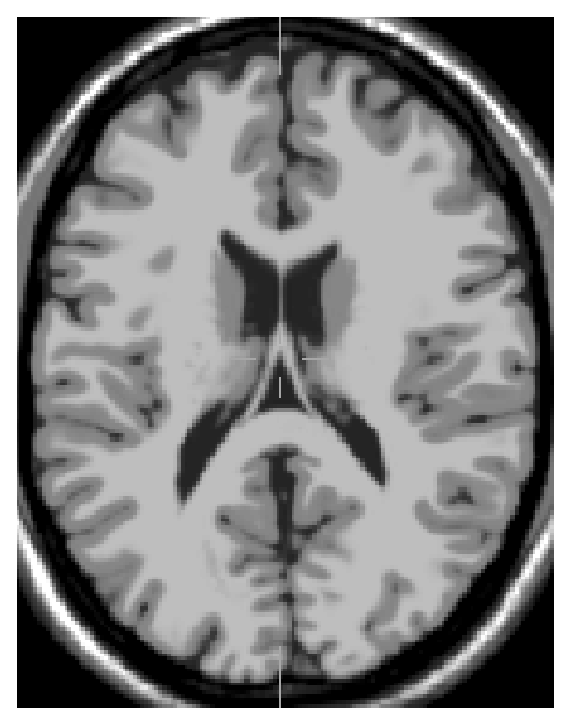
\includegraphics[width=32mm]{eps/chapitre2/original.eps}}
\hspace{1mm}
\subfigure[]{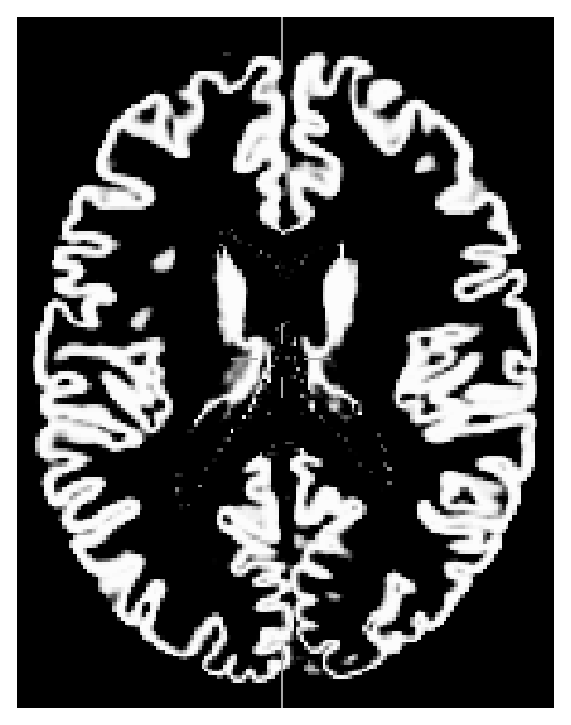
\includegraphics[width=32mm]{eps/chapitre2/gm_classic.eps}}
\hspace{1mm}
\subfigure[]{
\includegraphics[width=32mm]{eps/chapitre2/wm_classic.eps}}
\hspace{1mm}
\subfigure[]{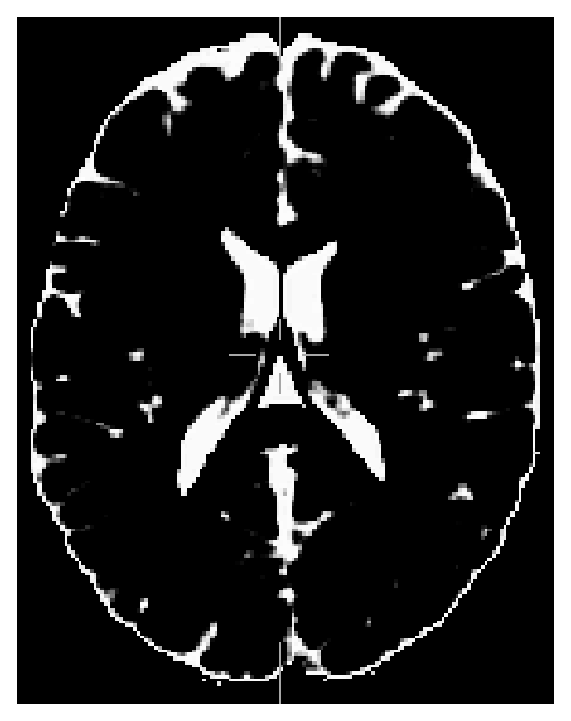
\includegraphics[width=32mm]{eps/chapitre2/csf_classic.eps}}
\caption{\emph{
Segmentation par FCM illustrant l'effet de volume partiel.
(a) Une coupe d'IRM c�r�brale.
(b--d) Segmentation de (a): (b) mati�re grise, (c) mati�re blanche, (d) LCR.
\label{FIG:EX:FCM:PVE}}}
%\end{figure}
\vspace{3mm}
%\begin{figure}[!htp]
\centering
\subfigure[]{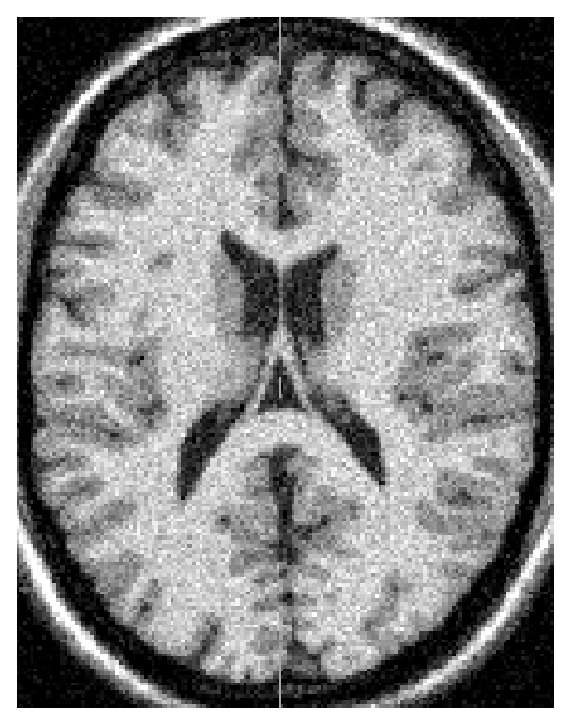
\includegraphics[width=32mm]{eps/chapitre2/original_noise.eps}}
\hspace{1mm}
\subfigure[]{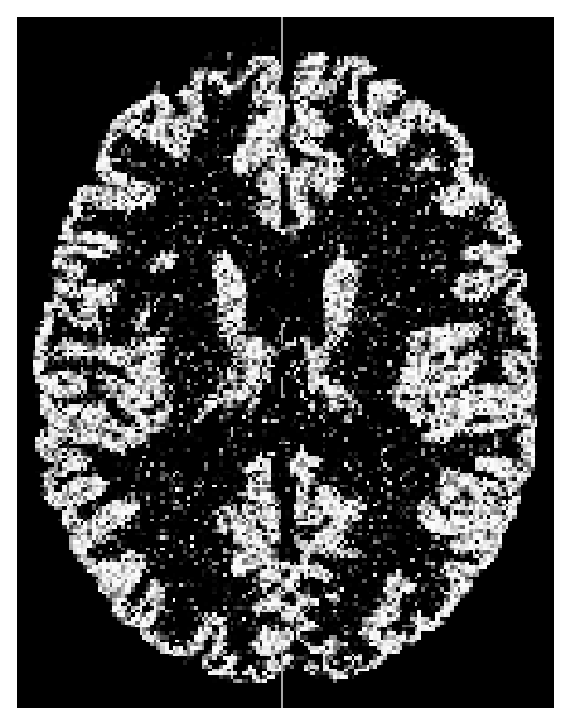
\includegraphics[width=32mm]{eps/chapitre2/gm_noise.eps}}
\hspace{1mm}
\subfigure[]{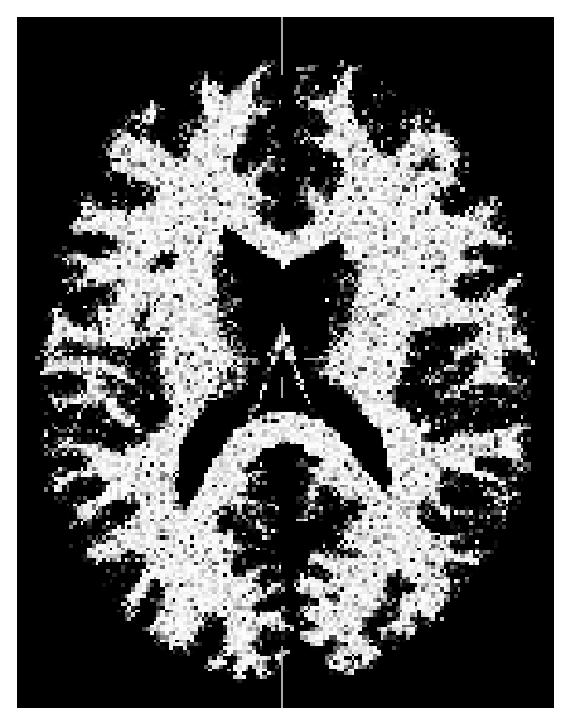
\includegraphics[width=32mm]{eps/chapitre2/wm_noise.eps}}
\hspace{1mm}
\subfigure[]{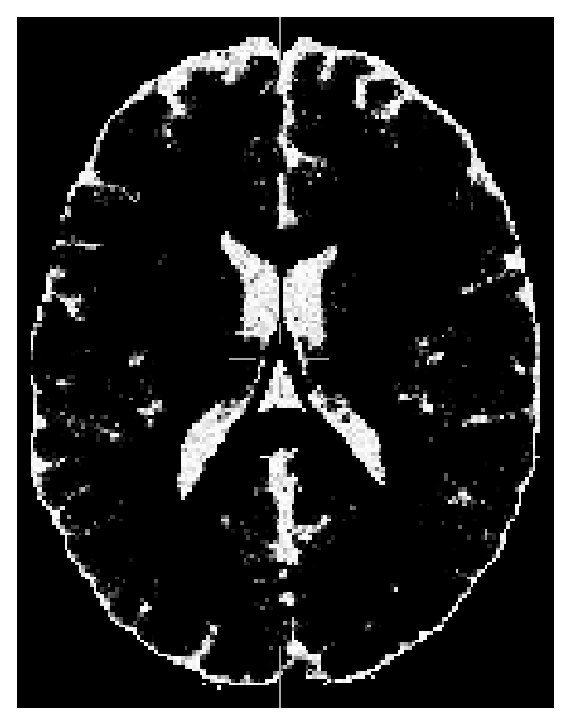
\includegraphics[width=32mm]{eps/chapitre2/csf_noise.eps}}
\caption{\emph{
Segmentation par FCM d'une image bruit�e.
(a) Une coupe d'IRM c�r�brale (similaire � celle de la Figure~\ref{FIG:EX:FCM:PVE}(a)) alt�r�e par un bruit.
(b--d) Segmentation de (a): (b) mati�re grise, (c) mati�re blanche, (d) LCR.
\label{FIG:EX:FCM:NOISE}}}
%\end{figure}
\vspace{3mm}
%\begin{figure}[!htp]
\centering
\subfigure[]{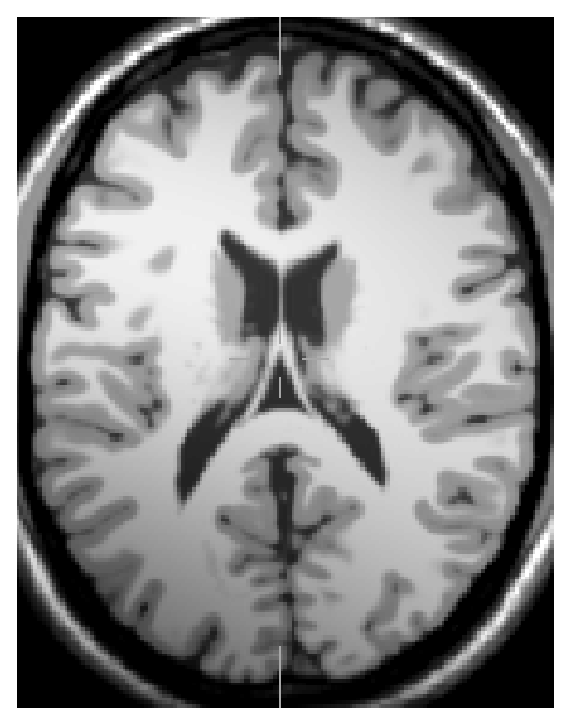
\includegraphics[width=32mm]{eps/chapitre2/original_bias.eps}}
\hspace{1mm}
\subfigure[]{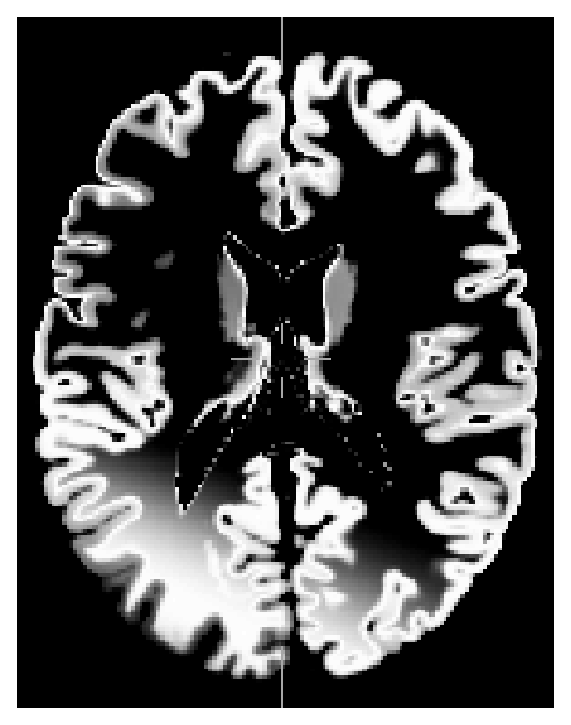
\includegraphics[width=32mm]{eps/chapitre2/gm_bias.eps}}
\hspace{1mm}
\subfigure[]{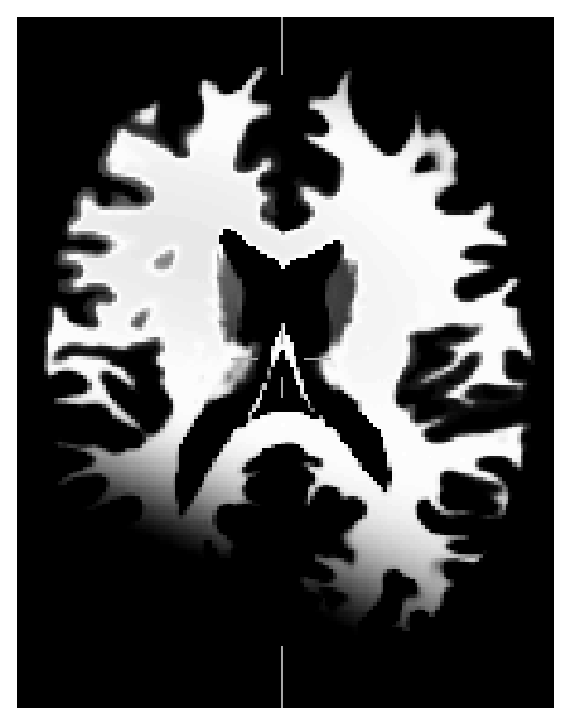
\includegraphics[width=32mm]{eps/chapitre2/wm_bias.eps}}
\hspace{1mm}
\subfigure[]{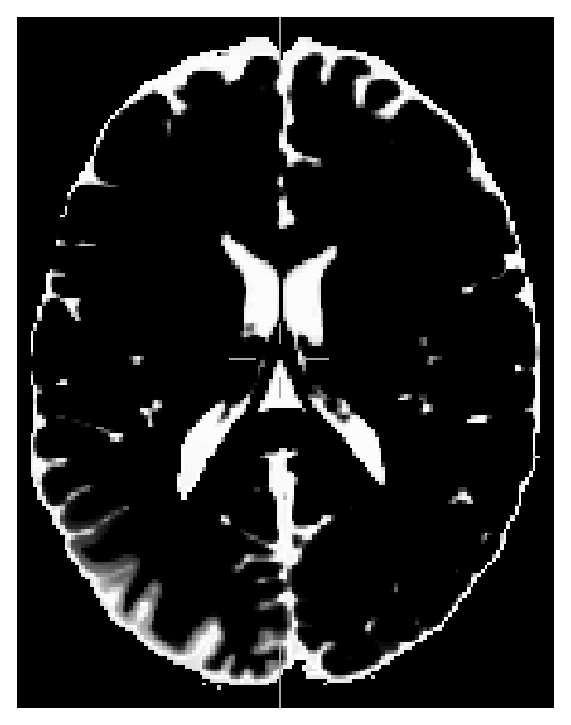
\includegraphics[width=32mm]{eps/chapitre2/csf_bias.eps}}
\caption{\emph{
Segmentation par FCM d'une image pr�sentant un biais en intensit�.
(a) Une coupe d'IRM c�r�brale (similaire � celle de la Figure~\ref{FIG:EX:FCM:PVE}(a)) alt�r�e par un biais.
(b--d) Segmentation de (a): (b) mati�re grise, (c) mati�re blanche, (d) LCR.
\label{FIG:EX:FCM:BIAS}}}
\end{figure*}

La premi�re d�finition de l'algorithme FCM remonte � l'article de \cite{Zadeh:IC:1965} et s'appuie sur la notion d'ensembles flous.
Tr�s vite, cet algorithme a trouv� des applications, notamment dans le cadre m�dicale, comme en t�moignent les publications de : \cite{Adey:IJN:1972}, \cite{Bezdek:NCC:1976} et \cite{Kalmanson:AJC:1975}.
Il part du principe qu'une donn�e n'a pas � �tre class�e dans une classe en particulier, mais � plusieurs avec un certain degr� d'appartenance.

L'algorithme FCM calcule une mesure de cette appartenance, via une fonction d'appartenance floue~\cite{Pham:IJPRAI:1996}, en chaque voxel de l'image et pour un nombre donn� de classes.
Soit une image $I : \Omega \rightarrow \mathbf{Y}$, o� $\Omega$ est le support de l'image et $\mathbf{Y}$ l'espace des intensit�s.
Il contient $N$ voxels, $\mathbf{x}_{j}$ et $\mathbf{y}_{j}$ repr�sentent respectivement les coordonn�es spatiales et l'intensit� du voxel $j$.

L'algorithme FCM effectue une s�rie d'it�ration entre l'�valuation de la fonction d'appartenance floue $u_{jk}$ et le calcul des centro�des des classes $\mathbf{v}_k$.
La fonction d'appartenance est calcul�e en chaque voxel et pour chaque classe.
Elle est contrainte de mani�re que $0 \leq u_{jk} \leq 1$ et que $\sum_{k=1}^{C} u_{jk} = 1$, o� $C$ est le nombre de classes.
Cette donn�e est suppos�e connue.
Un fort degr� d'appartenance (proche de $1$) signifie que l'intensit� du voxel consid�r� est proche du centro�de de la classe, ce dernier �tant consid�r� comme un prototype repr�sentatif de l'intensit� de la classe consid�r�e.

Math�matiquement, l'algorithme FCM se d�roule de la fa�on suivante : 
\begin{enumerate}
        \item Initialisation des centro�des (peut-�tre faite par un algorithme $k$-means, o� gr�ce � un atlas).
        \item Calcul de la fonction d'appartenance floue par $u_{jk} = \frac{D^{2}(\mathbf{y}_j, \mathbf{v}_k)}{\sum_{k=1}^{C} D^{2}(\mathbf{y}_j, \mathbf{v}_k)}$, o� $D^{2}(\mathbf{y}_j, \mathbf{v}_k)$ repr�sente une mesure de la similarit� entre l'intensit� au voxel $j$ et le centro�de de la classe $k$.
        \item Calcul des nouveaux centro�des : $\mathbf{v}_k = \frac{\sum_{i \in \Omega}u_{jk}\mathbf{y}_j}{\sum_{i \in \Omega}u_{jk}}$.
        \item Si il y'a convergence, arr�t de l'algorithme, sinon retour au point 2.
\end{enumerate}

Ces it�rations reviennent � effectuer un processus de minimisation de la fonction de co�t suivante : 
\begin{equation}
J_{FCM} = \sum_{j \in \Omega} \sum_{k=1}^{C} u^{q}_{jk} D^{2}(\mathbf{y}_{j},\mathbf{v}_{k}) \label{eq:fcm},
\end{equation}
o� $q$ est le degr� de flou de la segmentation, habituellement fix� � $2$ dans la litt�rature.
La convergence est atteinte lorsqu'un minimum local de cette fonction est d�tect�e.
De mani�re g�n�rale, le calcul de la similarit� entre l'intensit� des voxels et les centro�des des classes est r�alis� par la norme euclidienne, ce qui se traduit math�matiquement par : $D^{2}(\mathbf{y}_{j},\mathbf{v}_{k}) = \lVert \mathbf{y}_{j} - \mathbf{v}_{k} \rVert_{2}^{2}$.

L'hypoth�se fondamentale faite lors de l'utilisation de l'algorithme FCM en segmentation anatomique est que chaque tissu peut-�tre repr�sent� par une unique valeure $\mathbf{v}_k$, qui serait uniforme sur l'ensemble du domaine de l'image.
Les variations de cette \og vraie \fg{} valeur sont alors imput�s au biais de l'image, au bruit et � l'effet de volume partiel (m�lange de plusieurs tissus au sein d'un m�me voxel dont les proportions d�terminent l'intensit� du voxel).
Dans le cas de la segmentation anatomique adulte, cette hypoth�se est suffisante pour effectu�e la segmentation d'une IRM adulte, mais n�cessite l'int�gration de nouvelles donn�es de mani�re � prendre en compte le biais et le bruit.

\subsection{Autres m�triques utilis�es}
\label{subsec:fcm:dd}

Certains auteurs ont cherch� � �valuer l'impact d'une d�finition alternative de la mesure de similarit� entre l'intensit� des voxels et les centro�des des classes.
Deux grandes voies ont �t� suivies, la premi�re utilisant la distance de Mahalanobis (utile en cas d'utilisation de donn�es multi-spectrales) et la deuxi�me utilisant des op�rateurs noyaux de mani�re � projeter les donn�es dans un autre espace o� la segmentation serait plus ais�e.

Concernant l'utilisation des op�rateurs noyaux, un �tat de l'art g�n�rale de leur utilisation en clustering est fournit par~\cite{Filippone:PR:2008}.
L'int�ret des op�rateurs noyaux est leur capacit� � s�parer des donn�es non-lin�aires en projetant les donn�es dans un espace o� une s�paration lin�aire serait possible.
Une exemple de l'utilisation de ces op�rateurs est le \emph{Support Vector Machine} (SVM) qui est un algorithme de classification supervis�.

Formellement, les fonctions noyaux sont d�finis de la fa�on suivante.
Soit $X=\{\mathbf{x}_1,\ldots,\mathbf{x}_n\}$ un ensemble non vide avec $\mathbf{x}_i \in R^d$.
Une fonction $K : X \times X \rightarrow \mathbb{R}$ est un \emph{noyau d�fini positif} si et seulement si $K$ est sym�trique ($K(\mathbf{x}_i,\mathbf{x}_j) = K(\mathbf{x}_j,\mathbf{x}_i)$) et respecte l'�quation suivante :
$$
\sum_{i=1}^n\sum_{j=1}^n c_i c_j K(\mathbf{x}_i,\mathbf{x}_j) \geq 0 \ \forall n \geq 2,
$$
o� $c_r \in \mathbb{R}$, $\forall r = 1,\ldots,n.$

Chaque noyau peut �tre exprim� de la mani�re suivante :
$$
K(\mathbf{x}_i,\mathbf{x}_j) = \varPhi(\mathbf{x}_i)\cdotp\varPhi(\mathbf{x}_j),
$$
o� $\varPhi : X \rightarrow \mathcal{F}$ r�alise une transformation de l'espace de d�part $X$ vers un espace d'arriv�e $\mathcal{F}$ de plus grande dimension.
Cependant, un des aspects les plus int�ressants de cette transformation est qu'il est possible de calculer la distance euclidienne dans $\mathcal{F}$ sans pour autant conna�tre explicitement la transformation $\varPhi$.
En effet, cette distance est donn�e par :
$$
\lVert \varPhi(\mathbf{x}_i) - \varPhi(\mathbf{x}_j) \rVert^2 = K(\mathbf{x}_i,\mathbf{x}_i) + K(\mathbf{x}_j,\mathbf{x}_j) - 2K(\mathbf{x}_i,\mathbf{x}_j).
$$

Cette propri�t� des noyaux permet de d�finir deux versions de FCM.
La premi�re utilise une m�thode de \og kernalisation \fg{} de la m�trique~\cite{Zhang:AIM:2004}.
La fonction de co�t � minimiser devient alors : 
\begin{equation}
J_{FCM}^{\varPhi} = \sum_{j \in \Omega} \sum_{k=1}^{C} u^{q}_{jk} \lVert \varPhi(\mathbf{y}_{j}) - \varPhi(\mathbf{v}_{k}) \rVert_{2}^{2} \label{eq:fcm:kernel}.
\end{equation}
La fonction d'appartenance est alors calcul�e par $\frac{1}{u_{jk}} = \sum_{l=1}^{C} \left( \frac{1-K(\mathbf{y}_{j},\mathbf{v}_{k})}{1-K(\mathbf{y}_{j},\mathbf{v}_{l})} \right)$ et les centro�des par : $\mathbf{v}_k = \frac{\sum_{j \in \Omega} u_{jk}^q K(\mathbf{y}_j,\mathbf{v}_k)\mathbf{y}_j}{\sum_{j \in \Omega} u_{jk}^q K(\mathbf{y}_j,\mathbf{v}_k)}$.
La deuxi�me possibilit� est d'appliquer l'algorithme FCM directement dans l'espace d'arriv�e de la transformation $\varPhi$~\cite{Graepel:WFNS:1998}.

Une autre fa�on de modifier la mesure de similarit� et de trouver des fronti�res entre les classes plus pertinente est d'introduire la distance de Mahalanobis � la place de la distance euclidienne, ce qui revient � d�finir la mesure de similarit� comme~\cite{Gustafson:CDC:1978, He:CMIG:2008} :
$$
D^{2}(\mathbf{y}_{j},\mathbf{v}_{k}) = (\mathbf{y}_{j} - \mathbf{v}_k)^T T_k (\mathbf{y}_{j} - \mathbf{v}_k),
$$
o� $T_k$ est une matrice calcul�e � partir d'une matrice de covariance floue $S_k$ calcul�e de la fa�on suivante : 
$$
S_k = \frac{\sum_{j \in \Omega}u_{jk}^{q}(\mathbf{y}_j - \mathbf{v}_k)(\mathbf{y}_j - \mathbf{v}_k)^T}{\sum_{j \in \Omega}u_{jk}^{q}}.
$$
La matrice $T_k$ est d�duite de $S_k$ selon : $T_k = \sqrt{\lvert S_k \rvert} S_{k}^{-1}$.
Cette formulation a l'avantage de tenir compte d'une r�partition des donn�es autre qu'une r�partition sph�rique, comme l'hypoth�se est faite avec l'utilisation de la norme euclidienne.

Cependant, les formulations d�crites cherchent � obtenir une s�paration fiable des donn�es par l'utilisation d'un espace plus appropri�, mais ne prennent pas en compte la pr�sence de bruit dans l'image.
Deux approches sont int�ressantes car elles apportent une r�ponse � cette probl�matique par une d�finition de la similarit�.
Nous pouvons citer l'article de~\cite{Shen:TITB:2005}, qui inclue un m�canisme d'attraction du voisinage dans la d�finition de la similarit� en fonction du niveau de gris et de la distance au voxel courant. 
Afin de r�gler au mieux les param�tres contr�lant les poids respectifs de ces deux termes, une optimisation par un r�seau de neurones a �galement �t� mise en place.

La deuxi�me approche est un article de~\cite{Wang:MIA:2009}.
Elle consiste � r�aliser une analyse multi-�chelle de l'image.
Toute d'abord, un filtre de diffusion est appliqu� plusieurs fois � l'image � trait�, ce qui a pour effet d'obtenir une image avec un niveau de d�tails tr�s r�duit.
Par la suite, une segmentation de l'image la plus grossi�re est r�alis�e par FCM, et ce r�sultat est utilis� pour r�aliser la segmentation � un niveau de d�tails plus �lev� jusqu'� l'image originale.
Cette m�thode est int�ressante car elle utilise le m�me principe que la segmentation � l'aide d'un atlas statistique, mais �vite les probl�mes d'utilisation que peuvent poser un atlas comme le recalage et la construction de l'atlas lui-m�me.

\subsection{Mod�lisation du biais en intensit�}
\label{subsec:fcm:bias}

La prise en compte du biais en intensit� introduit par les imageurs est un probl�me qui a eu des r�ponses sp�cifiques et adapt�es � la formulation de l'algorithme FCM.
De mani�re g�n�rale, le signal re�u est mod�lis� comme le produit du \og vrai \fg{} signal et d'un champ de biais, supos� varier lentement le long du support de l'image.
Cependant, l'application d'une transform�e logarithmic � l'espace des intensit�s  permet de mod�liser le signal comme l'addition du vrai signal et du champ de biais, comme dans les travaux de~\cite{Ahmed:TMI:2002}.
L'intensit� est donc mod�lis�e par : $\mathbf{y}_j = \mathbf{\dot{y}}_j + b_j$, o� $\mathbf{\dot{y}}_j$ repr�sente la \og vraie \fg{} intensit� au voxel $j$ et $b_j$ repr�sente le biais au voxel $j$.
L'�valuation du biais repr�sente alors une �tape suppl�mentaire de l'algorithme FCM, apr�s l'�valuation des fonctions d'appartenance et des centro�des, et est faite de la fa�on suivante : $b_j = \mathbf{y}_{j} - \frac{\sum_{k=1}^{C}u^q_{jk}\mathbf{v}_k}{\sum_{k=1}^{C}u^q_{jk}}$.

Les travaux de~\cite{Liew:TMI:2003} exploite d'une mani�re diff�rente l'hypoth�se de faible variabilit� du biais.
Ce dernier est mod�lis� comme une pile de surfaces B-Splines.
Ainsi, le biais est �valu� par une surface par coupe de l'image avec une r�gularisation imposant une continuit� entre les diff�rentes coupes.
L'�valuation du biais est ainsi r�duite au calcul des coefficients contr�lant les diff�rentes surfaces.

Un autre exemple d'estimation du biais est donn� par les travaux de~\cite{Li:IPMI:2009}.
Ils introduisent un mod�le appel� un clustering des intensit� local et coh�rent (en anglais : \emph{coherent local intensity clustering} ou \emph{CLIC}) destin� � prendre en compte la similarit� des intensit� d'un voisinage.
Les voxels de ce voisinage sont pond�r�s � l'aide d'un noyau gaussien $K(\cdot)$ tronqu� de la forme : 
\begin{equation}
K(\mathbf{u}) = 
        \left\{
	\begin{array}{r c}
	        \exp{\frac{-\lvert \mathbf{u} \rvert^2}{2\sigma^2}} & \mbox{ pour } \lvert \mathbf{u} \rvert < \rho \\
	        0 & \mbox{sinon}
	\end{array}
        \right.
\end{equation}
o� $\rho$ est le rayon du voisinage pris en compte.
La fonction d'�nergie � minimiser devient donc : 
\begin{equation}
J = \sum_{j \in \Omega} \sum_{k = 1}^{C}u_{jk}^q \sum_{l \in \Omega} K(\mathbf{x}_j - \mathbf{x}_l) \lVert \mathbf{y}_{j} - b_{l}\mathbf{v}_{k} \rVert^2.
\end{equation}
L'avantage de cette formulation est que la prise en compte des intensit�s d'un voisinage autour du voxel courant permet �galement la correction du bruit de l'image, tout en ajoutant une pond�ration en fonction de la distance par rapport au voxel courant, partant du principe que seul les voxels les plus proches sont les plus pertinents � prendre en compte.

Tous ces mod�les utilisent une mod�lisation explicite du biais en intensit�, ajoutant une �tape suppl�mentaire d'estimation du biais en plus de l'estimation des centro�des et des fonctions d'appartenance.
De plus, les hypoth�ses sur la nature multiplicative du biais, ainsi que les faibles variations d'intensit� dues � ce ph�nom�ne restreignent sa prise en compte.

\subsection{Prise en compte du bruit}
\label{subsec:fcm:noise}

Au d�but des ann�es 2000, la n�cessit� d'une prise en compte du bruit produit par les imageurs a conduit � l'introduction de termes de r�gularisation dans la fonction d'�nergie de l'algorithme FCM.
L'id�e commune � ces m�thodes est l'utilisation de l'environnement autour d'un voxel pour contraindre sa segmentation.
Par exemple, si un voxel est au milieu d'une zone de mati�re blanche, le processus de segmentation va favoriser sa classification en mati�re blanche de mani�re � obtenir une continuit� des lables des tissus.

Dans cette optique, deux fonctions d'�nergie ont �t� d�finies de mani�re ind�pendante.
Elles d�finissent la fonction d'�nergie comme la somme d'un terme d'attache aux donn�es, correspondant � l'algorithme FCM classique, et d'un terme de r�gularisation tenant compte des fonctions d'appartenance des voxels voisins destin� � corriger les fonctions d'appartenance au voxel $j$ en fonction de cet environnement.
La premi�re, appel�e FCM robuste (en anglais : \emph{Robust FCM} ou \emph{RFCM})~\cite{Pham:CVIU:2001} ne prend en compte que les fonctions d'appartenance des voxels voisins pour contraindre la segmentation : 
\begin{equation}
J_{RFCM} = \sum_{j \in \Omega} \sum_{k=1}^{C} u^{q}_{jk} \lVert \mathbf{y}_{j} - \mathbf{v}_{k} \rVert_{2}^{2} + \frac{\beta}{2} \sum_{j \in \Omega} \sum_{k=1}^{C} u^{q}_{jk} \sum_{l \in N_j} \sum_{m \in M_k} u^q_{lm}  \label{eq:rfcm},
\end{equation}
o� $N_j$ repr�sente un voisinage du voxel courant $j$, $M_k = \{1,\ldots,C\} \backslash \{k\}$ et o� $\beta$ contr�le les poids respectifs du terme d'attache aux donn�es et du terme de r�gularisation.
La deuxi�me m�thodologie, appel�e un FCM modifi� (en anglais : \emph{Modified FCM} ou \emph{MFCM})~\cite{Ahmed:TMI:2002},  d�finie la fonction d'�nergie de la fa�on suivante : 
\begin{equation}
J_{RFCM} = \sum_{j \in \Omega} \sum_{k=1}^{C} u^{q}_{jk} \lVert \mathbf{y}_{j} - \mathbf{v}_{k} \rVert_{2}^{2} + \frac{\beta}{\lvert N_j \rvert} \sum_{j \in \Omega} \sum_{k=1}^{C} u^{q}_{jk} \sum_{l \in N_j} \lVert \mathbf{y}_{j} - \mathbf{v}_{k} \rVert^{2}_{2}  \label{eq:mfcm}. 
\end{equation}

La principale diff�rence entre ces deux formulations de la r�gularisation r�side dans l'exploitation du voisinage.
L'algorithme RFCM effectue une r�gularisation enti�rement fond�e sur les fonctions d'appartenance, encourageant d'autant plus le lissage de ces fonctions au dur et � mesure des it�rations du l'algorithme.
De plus, le lissage de la fonction d'appartenance d'une classe $k$ ne tient compte que des fonctions des autres classes, la logique �tant que plus la proportion d'autre classes dans l'environnement est importante, plus la classe courante doit �tre p�nalis�e de mani�re � favoriser les autres classes.
Ceci est illustr� par le calcul de la fonction d'appartenance qui s'exprime de la fa�on suivante : 
\begin{equation}
u_{jk} = \frac{(\lVert \mathbf{y}_{j} - \mathbf{v}_k \rVert_{2}^{2} + \beta \sum_{l \in N_j} \sum_{m \in M_k} u^{q}_{lm})^{-1}}{\sum_{i = 1}^{C}(\lVert \mathbf{y}_{j} - \mathbf{v}_i \rVert_{2}^{2} + \beta \sum_{l \in N_j} \sum_{m \in M_i}u^{q}_{lm})^{-1}}.\label{eq:rfcm:u}
\end{equation}
La forte pr�sence d'autres classes dans le voisinage autour du voxel $j$ entraine une diminution du d�nominateur, diminuant d'autant l'appartenance � la classe courante.
A l'inverse, si une forte proportion de la classe courante est pr�sente dans le voisinage, alors seul le terme d'attache aux donn�es est consid�r�.

L'algorithme MFCM effectue une r�gularisation par rapport � la similarit� entre l'intensit� des voxels voisins et le centro�de de la classe courante.
L'analyse de l'expression des fonctions d'appartenance donn�e par l'�quation \ref{eq:mfcm:u} :
\begin{equation}
u_{jk} = \frac{(\lVert \mathbf{y}_{j} - \mathbf{v}_k \rVert_{2}^{2} + \beta \sum_{l \in N_j} \lVert \mathbf{y}_{l} - \mathbf{v}_{k} \rVert_{2}^{2})^{-1}}{\sum_{i = 1}^{C}(\lVert \mathbf{y}_{j} - \mathbf{v}_i \rVert_{2}^{2} + \beta \sum_{l \in N_j} \lVert \mathbf{y}_{l} - \mathbf{v}_{i} \rVert_{2}^{2})^{-1}} \label{eq:mfcm:u},
\end{equation}
montre que l'ajout de ce terme de r�gularisation entraine une diminution du d�nominateur si l'intensit� des voxels voisins est trop dissemblables de la valeur du centro�de.
Le calcul des centro�des doit prendre en compte le voisinage d�fini et est donc exprim� de la fa�on suivante : 
\begin{equation}
\mathbf{v}_k = \frac{\sum_{k=1}^{C} u_{jk}^{q} \left( \mathbf{y}_{j} + \frac{\beta}{\lvert N_j \rvert} \sum_{l \in N_j} \mathbf{y}_l \right)}{(1+\beta) \sum_{k=1}^{C} u_{jk}^{q}}
\end{equation}


L'exploration des diff�rents voisinage �tant couteuse en temps de calcul, des am�liorations visant l'acc�l�ration de l'ex�cution ont �t� mise en place.
Les travaux de~\cite{Szilagyi:AICIEEE:2003} parviennent � ce but en d�finissant une image interm�diaire $\zeta$ d�finie de la mani�re suivante : 
\begin{equation}
\mathbf{\zeta}_{j} = \frac{1}{1+\beta} \left( \mathbf{y}_{j} + \frac{\beta}{\lvert N_j \rvert} \sum_{l \in N_j} \mathbf{y}_{l} \right) \label{eq:Szilagyi:Image}.
\end{equation}
De plus, afin de ne pas explorer l'image plusieurs fois au cours des it�rations de l'algorithme, un param�tre $\gamma_{p}$ est introduit indiquant le nombre de voxels de l'image � une intensit� $p$ donn�e (par cons�quent, on a bien $\sum_{p = 0}^{p_{max}} \gamma_{p} = N$).
La fonction d'�nergie � minimiser s'exprime donc de la fa�on suivante : 
\begin{equation}
J_{EnFCM} = \sum_{p=0}^{p_{max}} \sum_{k=1}^{C} \gamma_{p} u_{pk}^{q} \lVert \mathbf{\zeta}_{p} - \mathbf{v}_{k} \rVert_{2}^{2} \label{eq:Szilagyi:Cost}.
\end{equation}
Le calcul des fonctions d'appartenance est le m�me que pour l'algorithme FCM classique, la diff�rence se situant lors du calcul des centro�des, devant tenir compte du nombre de voxel � une intensit� donn�e.
Les centro�des sont donc exprim�s selon : 
\begin{equation}
\mathbf{v}_{k} = \frac{\sum_{p = 0}^{p_{max}} \gamma_{p} u_{pk}^{q} \zeta_{p}}{\sum_{p = 0}^{p_{max}} \gamma_{p} u_{pk}^{q}} \label{eq:Szilagyi:centroid}.
\end{equation}
Les avantages de cette m�thodologie sont donc un traitement acc�l�r� ainsi qu'une approche beaucoup plus similaire au FCM classique.
De plus, les auteurs montrent que leur algorithme converge plus vite (en moins d'it�rations) que la version MFCM.

Toujours en suivant la m�me id�e d'acc�l�rer l'ex�cution d'un algorithme FCM ayant un terme de r�gularisation, les travaux de~\cite{Chen:TSMC:2004} introduisent la moyenne ou la m�diane du voisinage plut�t que le calcul d'une image compl�te pour se ramener au cas de l'algorithme FCM classique.
De plus, ils ajoutent l'utilisation d'un noyau gaussien de mani�re � ajouter une robustesse au bruit et aux \emph{outliers}.
Cet algorithme est appel� le KFCM\_S est la fonction co�t � minimiser devient : 
\begin{equation}
J_{KFCM\_S} = \sum_{j \in \Omega} \sum_{k=1}^{C} u^{q}_{jk} (1 - K(\mathbf{y}_j, \mathbf{v}_k)) + \beta \sum_{j \in \Omega} \sum_{k=1}^{C} u^{q}_{jk} (1 - K(\mathbf{\overline{y}}_j, \mathbf{v}_k)),
\end{equation}
o� $\mathbf{\overline{y}}_j$ repr�sente la moyenne ou la m�diane des intensit�s dans le voisinage $N_j$.
L'expression des fonctions d'appartenance et des centro�des est similaire � celle de~\cite{Ahmed:TMI:2002}.
Il existe �galement une version de cet algorithme n'utilisant pas les op�rateurs noyaux, appel� FCM\_S.
% Il suffit de remplacer le terme $\lVert \mathbf{y}_j - \mathbf{v}_k \rVert^{2}_{2}$ par $(1-K(\mathbf{y}_j, \mathbf{v}_k))$ dans le calcul de la fonction d'appartenance.

Cependant, les deux m�thodes pr�c�dentes, tout comme les m�thodes de~\cite{Ahmed:TMI:2002} et \cite{Pham:CVIU:2001}, ont le d�savantage de reposer sur un param�tre $\beta$ contr�lant les poids respectifs entre les termes d'attache aux donn�es et le terme de r�gularisation.
Ce param�tre est choisi la plupart du temps par exp�rimentation et ce choix est loin d'�tre intuitif.
De plus, comme dit pr�c�demment, ces algorithmes peuvent devenir tr�s gourmand en temps de calcul � cause de l'exploration des voisinages.
Les travaux de~\cite{Cai:PR:2007} d�finissent un algorithme FCM g�n�ralis� (FGFCM) d�finissant une image interm�diaire comme d�crit dans l'article de~\cite{Szilagyi:AICIEEE:2003} de mani�re � diminuer les temps de calcul et introduisent une fa�on d'�valuer localement le poid � attribuer au terme de r�gularisation en fonction de la position spatiale des voxels et de la similarit� des intensit�s.
Ce param�tre de r�gularisation locale $S_{jl}$ est d�fini de la fa�on suivante : 
\begin{equation}
S_{jl} = \left\{
        \begin{array}{l r}
	S_{s\_jl} \times S_{g\_jl}, & j \neq l, \\
	0, & j = l,
        \end{array}
\right.
\end{equation}
o� $S_{s\_jl}$ contr�le la relation spatiale entre les voxels $j$ et $l$ et $S_{g\_jl}$ est fonction de la similarit� entre ces deux voxels.
Le param�tre $S_{s\_jl}$ est d�fini de la fa�on suivante : 
\begin{equation}
S_{s\_jl} = \exp \left( \frac{-\lVert \mathbf{x}_i - \mathbf{x}_l \rVert}{\lambda_s} \right),
\end{equation}
et le param�tre $S_{g\_jl}$ de la fa�on suivante : 
\begin{equation}
S_{g\_jl} = \exp \left( \frac{-\lVert \mathbf{y}_j - \mathbf{y}_l \rVert^{2}}{\lambda_g \times \sigma^{2}_{g\_i}} \right),
\end{equation}
o� $\sigma_{g\_i}$ est d�fini comme l'�cart moyen entre l'intensit� des voxels voisins et le voxel courant.
Ce param�tre est d�fini de la fa�on suivante : 
\begin{equation}
\sigma^{2}_{g\_i} = \frac{\sum_{l \in N_j} \lVert \mathbf{y}_j - \mathbf{y}_l \rVert^{2}}{\lvert N_j \rvert}.
\end{equation}
De cette mani�re, plut�t que d'avoir � fixer un param�tre de r�gularisation global $\beta$, deux param�tres $\lambda_g$ et $\lambda_s$ dont la d�finition est plus intuitive.
Le param�tre $\lambda_s$ peut �tre d�duit de la taille du voisinage utilis�, laissant $\lambda_g$ comme seul param�tre global � ajuster.
Avec cette d�finition du param�tre de r�gularisation local, il est alors possible de construire une image $\zeta$ selon la formule : 
\begin{equation}
\zeta_{j} = \frac{\sum_{l \in N_j} S_{jl} \mathbf{y}_{j}}{\sum{S_{jl}}}.
\end{equation}
La recherche du minimum de la fonction co�t se fait alors selon le m�me principe que les travaux de~\cite{Szilagyi:AICIEEE:2003}.

Une derni�re m�thode est � mettre en valeur. 
Constatant que le choix des param�tres de r�gularisation reste malgr� tout difficile (surtout en l'absence d'\emph{a priori} sur le bruit), les travaux de~\cite{Krinidis:TIP:2010} introduisent un nouveau facteur permettant de d�finir une r�gularisation sans param�tre contr�lant le poids entre l'attache aux donn�es et la r�gularisation.
Ce facteur, not� $G_{jk}$, est calcul� de la fa�on suivante : 
\begin{equation}
G_{jk} = \sum_{l \in N_{j},\mbox{ }j \neq l} \frac{1}{\lVert \mathbf{x}_j - \mathbf{x}_l \rVert + 1} (1 - u^{q}_{lk}) \lVert \mathbf{y}_j - \mathbf{v}_k \rVert^{2}_{2}.
\end{equation}
La fonction co�t � minimiser devient alors : 
\begin{equation}
J_{FLICM} = \sum_{j \in \Omega} \sum_{k=1}^{C} (u_{jk}^{q} \lVert \mathbf{y}_{j} - \mathbf{v}_{k} \rVert^{2}_{2} + G_{jk}).
\end{equation}
La principale remarque est qu'il n'y a pas de param�tre r�glant le poids entre l'attache aux donn�es et la r�gularisation.
Le poids de la r�gularisation est d�termin� de mani�re compl�tement automatique en fonction de la similarit� en intensit� et de la position spatiale des voxels consid�r�s.
De plus, l'algorithme FLICM travaille directement sur l'image originale et prend en compte la mise � jour des fonctions d'appartenance � chaque it�ration, �vitant ainsi la perte de d�tails que peut occasionner le calcul d'une image moyenne.


%------------------------------------------------------------------------Maturation c�r�brale----------------------------------------------------------------------------------------


\section{Segmentation c�r�brale pr� et post-natales}

Cette section pr�sente un �tat de l'art en segmentation des cerveaux en maturation.
Elle concerne les m�thodes employ�es pour effectuer une segmentation des tissus c�r�braux dans les cas pr�nataux et post-nataux.
Ces derniers regroupent plusieurs cas distincts, notamment les pr�matur�s ou les jeunes enfants ag�s de moins de deux ans.

\subsection{Post-natal}

Une premi�re �tude concernant les tissus c�r�braux chez les enfants a �t� effectu�e par~\cite{Matsuzawa:CC:2001} et comprends des cas allant de 1 mois � 10 ans.
Il s'agit d'une �tude volum�trique cherchant � diff�rencier le LCR, la mati�re grise et la mati�re blanche.
Cependant, cette �tude ne prend pas en compte un �l�ment capital et qui est la my�linisation de la mati�re blanche au cours du temps.

Afin de palier � ce d�faut, les travaux de~\cite{Prastawa:MIA:2005} ont introduit une s�paration de la amti�re blanche my�linis�e et non my�linis�e.
Leur m�thode sur trois �tapes distincts �tant : l'estimation initiale de la distribution en intensit�, la correction du biais, puis la correction de la segmentation.
L'estimation initiale de la distribution en intensit� est r�alis� gr�ce � un seuillage d'un atlas anatomique pr�alablement recal� sur le cas � traiter.
Ce seuillage permet de collecter des �chantillons de LCR, de mati�re grise et de mati�re blanche.
L'estimation de la distribution en intensit� du LCR et de la mati�re grise est faite directement, tandis que la distribution de la mati�re blanche my�linis�e et non my�linis�e est obtenue par �lagage d'un arbre minimum construit � partir des �chantillons des deux types de mati�re blanche.
La correction du biais est obtenue selon la m�thode de~\cite{VanLeemput1:TMI:1999}.
La derni�re �tape est r�alis� par l'utilisation d'une m�thode d'estimation de la distribution en intensit� non-param�trique � cause notamment des forts recouvrements dues � une mod�lisation gaussienne.
Une nouvelle fois, des �chantillons fiables sont tir�s de l'image et permettent une estimation de la distribution en intensit� par l'utilisation de fonctions noyaux.

L'�tude de~\cite{Xue:NeuroImage:2007} a pour objectif d'�tudier l'�volution de la courbure du cortex au cours de la grossesse, ainsi que l'�volution de l'�paisseur corticale.
Les images utilis�es sont des images de pr�matur�s.
Pour atteindre cet objectif, une phase de segmentation des tissus, suivie d'une phase de reconstruction 3D du cortex est r�alis�e.
La phase de segmentation pr�sente �galement plusieurs �tape.
Une premi�re �tape �limine les tissus non-pertinents (tronc c�r�bral, cervelet, noyaux gris et corps caleux) dont l'intensit� est trop proche de celle du cortex.
Cette �tape est r�alis�e par le recalage d'un atlas, choisi en fonction de l'�ge de gestation du nouveau n�s.
La deuxi�me �tape consiste en une segmentation bas�e sur un algorithme EM permettant une premi�re segmentation du cortex et de la mati�re blanche.
Cependant, les effets de volume partiel propres aux images de nouveaux n�s n�cessite une troisi�me �tape permettant de d�tecter et de corriger les voxels ayant une mauvaise classification.
Cela est r�alis� par l'utilisation d'un algorithme EM int�grant des \emph{a priori} issu des champs de Markov.
Cependant, le poids de cette r�gularisation est modifi� en fonction de l'environnement entourant le voxel.
Par exemple, si un voxel est lab�lis� en temps que mati�re blanche mais qu'il est entour� de mati�re grise et de LCR, il est consid�r� comme �tant un voxel de volume partiel et l'\emph{a priori} markovien sera modifi� de mani�re � favoriser la mati�re grise et le LCR plut�t que la mati�re blanche.
En r�sum�, la segmentation du cortex est obtenue par une restriction de l'ensemble de segmentation puis par l'utilisation d'\emph{a priori} markoviens locaux, permettant une segmentation plus fiable du cortex.

Les travaux de~\cite{Weisenfeld:NeuroImage:2009} parviennent � une segmentation compl�te des structures c�r�brales par l'utilisation d'un estimation non-param�trique de la distribution d'intensit�.
Le pr�alable � cette segmentation est la mise � disposition d'une base d'images o� un expert a s�lectionn� plusieurs voxels repr�sentatifs des diff�rents tissus.
Ces voxels sont d�sign�s comme des prototypes et chaque image en a plusieurs milliers.
Chaque image de la base est alors recal�e sur le cas � �tudier et les prototypes vont permettre la d�finition de plusieurs segmentations et d'obtenir une classification floue de chaque tissu.
Les prototypes sont alors mis � jour et la segmentation r�estim� jusqu'� ce que la segmentation finale ne bouge plus.

L'approche de~\cite{Merisaari:JNM:2009} est int�ressante car elle ne repose que sur les donn�es de l'image pour effectuer la segmentation, malgr� qu'elle n'effectue que la s�paration du LCR du reste des structures c�r�brales.
Cette m�thode consiste en trois �tapes.
Premi�rement, une segmentation d�finissant de nombreuses zones est r�alis�e gr�ce � une segmentation par ligne de partage des eaux. 
Dans un deuxi�me temps, chaque zone est lab�lis�e selon le mod�le des mixtures de gaussienne en fonction de la moyenne des intensit�s de cette zone.
Enfin, cette premi�re segmentation est utilis�e comme \emph{a priori} de la m�me mani�re qu'un atlas pour effectuer la classification voxel par voxel.
Il s'agit de la premi�re approche cherchant � obtenir une segmentation sans phase d'apprentissage, ni atlas.

Plus r�cemment, l'article de~\cite{Shi:NeuroImage:2010} d�crit une approche longitudinale de la segmentation.
Partant du principe que des IRM acquises � un �ge plus avanc� seront plus pr�cises, notamment gr�ce � une plus grande maturit� des tissus, cette m�thodologie utilise les r�sultats d'une segmentation � un instant $t$ comme \emph{a priori} spatial pour obtenir une segmentation � un instant $t - 1$.
La premi�re segmentation est r�alis�e en utilisant l'algorithme AFCM de~\cite{Pham:TMI:1999} et les cartes de probabilit� issues de cette �tape sont ensuite recal�s sur les acquisition plus anciennes afin d'�tre segment� par un algorithme EM.

Du m�me auteur~\cite{Shi:HBM:2011}, nous pouvons �galement mentionner une m�thodologie destin�e � mettre le cortex en valeur.
Elle utilise un atlas de population mais le pond�re par des �l�ments du cas �tudi�, notamment une carte de confiance sur l'emplacement du cortex, issu d'un filtre hessien.
De plus, les �l�ments subcorticaux sur volumes intracr�nien sont enlev� � l'aide d'un template recal� sur le cas �tudi�, de mani�re � ne pas confondre les noyaux gris et le cortex.

De mani�re g�n�rale, les propri�t�s de IRM c�r�brales des nouveaux n�s ne permettent pas l'utilisation d'algorithmes de segmentation sans l'aide d'\emph{a priori} spatiaux sous forme d'atlas de population, ou sans l'ajout d'une phase d'apprentissage.
Cependant, une m�thode parue r�cemment est parvenue � une segmentation sans ces �l�ments en utilisant des \emph{ apriori} anatomiques g�n�riques.
L'article de~\cite{Gui:ISBI:2011} montre qu'il est possible d'obtenir une segmentation en ne se basant que sur les donn�es de l'images par une succession d'op�rations connues, mais mise en \oe uvre dans l'ordre n�cessaire � l'optention d'une segmentation compl�te.
L'extraction du volume intracr�nien, la division des deux h�misph�res c�r�braux et la d�tection des noyaux gris est r�alis�e gr�ce � une segmentation par ligne de partage des eaux.
Par la suite, l'extraction du cortex et de la mati�re blanche est r�alis� par un algorithme de croissance de r�gion avec des contraintes fortes telles que l'interdiction aux labels de LCR et de mati�re blanche d'�tre voisins.
De plus, une �tape finale de classification permet de segmenter le cervelet, le tronc c�r�bral et de d�tecter la mati�re blanche non-my�linis�e.
Cette m�thode semble performante mais est d�pend largement de la d�tection des noyaux gris.
Si les noyaux gris ne sont pas discernables, la segmentation n'est pas possible.

\subsection{Pr�natal}
\label{prenatal}

Les images acquises \emph{in utero} pr�sentent des difficult�s suppl�mentaires, dues au temps d'acquisition plus faible et au conditions d'acquisition particuli�re (impossibilit� d'immobilis� le patient, signal perturb� par les diff�rents tissus de la m�re, \ldots).
Cependant, l'�tude de la maturation c�r�brale \emph{in vivo} ainsi que la d�finition d'outils diagnostiques pr�nataux n�cessite la d�finition d'outils permettant de traiter automatiquement ces images.

Une premi�re tentative de segmentation des tissus c�r�braux est la m�thode de~\cite{Claude:TBE:2004}, consistant en une segmentation semi-autmatique.
Le but �tait de conduire une �tude de la fosse post�rieure du cr�ne et des structures comme le cervelet et le tronc c�r�bral.
La segmentation de la fosse post�rieure du cr�ne est r�alis�e de mani�re manuelle car il n'existe pas de d�limitation claire entre cette zone et le reste cerveau.
Le cervelet et le tronc c�r�bral sont segment�s gr�ce � un algorithme de croissance de r�gion.
Les germes sont choisies par un seuillage de l'image originale et la croissance est contr�l� par des crit�res d'adjacence et d'homog�n�it�.
Cette �tude est une premi�re tentative de segmentation des tissus c�r�braux en IRM f\oe tale.
Cependant, elle n'est r�alis� que sur une coupe sagittale et n�cessite une importante implication de l'expert pour d�limiter la fosse post�rieure du cr�ne.

Plus tard, les travaux de~\cite{Ferrario:ESPC:2008} se sont int�ress� � la reconstruction de la surface corticale des cerveaux de f\oe tus.
Pour parvenir � ce r�sultat, une premi�re �tape est l'extraction du volume intracr�nien faite gr�ce � un algorithme fond� sur les contours actifs~\cite{Bresson:JMIV:2007}.
La deuxi�me �tape consiste en une segmentation par mixtures de gaussiennes.
Deux classes de LCR, deux classes pour les tissus c�r�braux ainsi qu'une classe interm�diaire sont utilis�es afin de tenir compte du recouvrement des distributions d'intensit� des diff�rents tissus.
La classe interm�diaire est ensuite �limin�e par un algorithme de correction des labels fond� sur les champs de Markov favorisant les classes LCR et c�r�brales.
La troisi�me �tape consiste � rep�rer les deux  composantes connexes de LCR les plus grandes et d'�liminer la plus large de mani�re � obtenir la surface du cortex.

Les travaux de~\cite{Anquez:ISBI:2009} pr�sentent une m�thode d'extraction du volume intracr�nien, en utilisant des \emph{a priori} anatomiques ainsi que des op�rateurs de morphologie math�matique~\cite{Najman:2010}.
La premi�re �tape est une d�tection des yeux du f\oe tus � partir d'un mod�le comprenant des \emph{a priori} de forme, de contrastes ainsi que des \emph{a priori} biom�triques.
A partir de cette localisation des yeux, la coupe sagital passant au milieu du cerveau est reconstruite (l'orientation du sujet n'est pas connue) et une premi�re segmentation du volume intracr�nien est effectu�e dans cette coupe.
Cette premi�re segmentation est alors utilis�e pour contraindre la segmentation 3D dans une zone restreinte avant une segmentation compl�te par �l�gage d'un graphe.

Une autre m�thode de comprenant une phase de segmentation par mixture de gaussienne suivie d'une phase de r�gularisation d�connect�e des donn�es est celle de~\cite{BachCuedra:MICCAI:2009}.
Le but est cette fois de segmenter l'ensemble des tissus c�r�braux en distinguant les noyaux gris du cortex.
La premi�re �tape consiste en un algorithme EM divisant les voxels en huit classes (quatre classes pures et quatre classes de transition).
Le mod�le de Markov mis en \oe uvre est similaire � celui de~\cite{Ferrario:ESPC:2008} et est appliqu� trois fois successives.
La premi�re fois permet de labeliser tous les voxels voisins du fond de l'image comme �tant du LCR, la deuxi�me permet de segmenter le cortex en imposant un crit�re d'�paisseur et la troisi�me permet de s�parer les noyaux gris du cortex et de classer les voxels de transition encore pr�sent.
Cette m�thode est int�ressante car elle introduit des contraintes anatomiques, cependant la phase de r�gularisation d�connect�e des donn�es n'est pas sans poser quelques probl�mes car rien ne garantie que la segmentation peut se corriger automatiquement si elle n'est pas guid�e par les donn�es de l'image.

Les m�thodes suivantes b�n�ficient d'une �tape de reconstruction des volumes afin d'obtenir des images isotropes~\cite{Kim:TMI:2010,Rousseau:AR:2006}.

Une approche par atlas a �t� utilis�e par~\cite{Habas:SPIE:2009}.
Afin de b�n�ficier d'un \emph{a priori} suppl�mentaire sur le positionnement des tissus.
Sachant que le cerveau des f\oe tus se pr�sente sous la forme d'une succession de couches, ils utilisent cette connaissance pour b�tir un \emph{a priori} spatial sous une forme laminaire � partir d'une segmentation des ventricules et du LCR p�ric�r�bral. 
La connaissance des ventricules est issue d'un atlas anatomique construit sp�cifiquement pour cette application permettant d'avoir une connaissance des ventricules, de la matrice germinale, de la mati�re blanche, du cortex et du LCR p�ric�r�bral.
L'ensemble de ces connaissances est int�gr�e dans un algorithme EM avec une r�gularisation par champs de Markov cach�s.

Une m�thode plus r�cente~\cite{Gholipour:IJCARS:2011} n'utilise pas d'atlas anatomique, mais n'a pas pour objectif une segmentation des tissus.
L'objectif est de r�aliser une �tude quantitative du volume intracr�nien en supprimant le LCR p�ric�r�bral.
Plusieurs �tapes sont n�cessaires pour obtenir une segmentation de ce volume.
Dans un premier temps, une classification des voxels en dix classes est r�alis�e de mani�re � prendre en compte le recouvrement des distributions en intensit�.
A cette �tape, l'utilisateur doit s�lectionner les labels repr�sentant les tissus c�r�braux � cause de la variabilit� d'un cas � un autre.
Une fois les labels s�lectionn�s, un filtre morphologique est utilis� pour �liminer les voxels de volumes partiels ainsi que pour combler la partie du volume intracr�nien correspondant aux ventricules.
Enfin, un algorithme de contours actifs est appliqu� afin d'obtenir une segmentation finale.
Cette m�thodologie utilise des op�rateurs connus et n'est pas compl�tement automatique, cependant elle atteint son but de r�aliser une segmentation fiable du volume intracr�nien.

Une derni�re m�thodologie de segmentation des tissus est celle de~\cite{Habas:NeuroImage:2010}.
Ils pr�sentent la construction d'un atlas spatio-temporel afin de prendre les �volutions du cerveau au cours de la grossesse et de b�n�ficier d'un \emph{a priori} le plus pertinent possible.
Une utilisation de cet atlas dans le cadre de la segmentation c�r�brale est �galement pr�sent�e.


%------------------------------------------------------------------------Bilan----------------------------------------------------------------------------------------

\section{Bilan}
Positionnement des travaux.

\chapter[Contribution � l'algorithme des C-moyennes floues]{Contribution � l'algorithme des C-moyennes floues et application � la segmentation c�r�brale}
\label{chap:nlfcm}
\minitoc

Dans ce chapitre, une nouvelle m�thode de segmentation bas�e sur FCM est d�finie.
Elle inclue l'approche des moyennes non-locales (en anglais, \emph{non-local means}) propos�e en 2005.
Issue de travaux dans le cadre du d�bruitage d'images, cette derni�re a �t� sp�cifi�e de mani�re ind�pendante par \cite{Buades:MMS:2005}, et \cite{Awate:PAMI:2006}.
L'id�e g�n�rale est de profiter de la redondance de l'information au sein d'une image pour estimer la \og vrai \fg{} valeur en chaque voxel.
La n�cessit� d'avoir une �valuation robuste de ces similarit�s entre voxels a conduit � prendre en compte leur proche voisinage, conduisant � la d�finition de patches.

L'utilisation de la redondance de l'information de l'image est une option peu explor�e en segmentation c�r�brale.
Comme nous l'avons vu pr�c�demment, de nombreuses m�thodes utilisent une mod�lisation sp�cifique d'un champ de biais pour la correction de l'inhomog�n�it� de l'intensit� ou une approche prenant en compte la classification des voxels environnants pour la prise en compte du bruit.
Certaines m�thodologies de types FCM ont inclu une prise en compte de la redondance de l'information en favorisant les voxels dont l'intensit� et les coordon�es spatiales sont les plus proches de celles du voxel courant (voir en Section~\ref{subsubsec:fcm:ponderation}).
Cependant, les travaux sur les m�thodes de d�bruitage par patches (dont l'approche non-locale) ont montr� que ces derni�res �taient efficaces car elles offrent une estimation de la similarit� plus fiable qu'une comparaison de la seule valeur des voxels~\cite{Salmon:2010}.
Un terme de r�gularisation non-local int�gre don une meilleure prise en compte de l'environnement autour du voxel courant pour effectuer la r�gularisation.

Concernant la prise en compte du biais, une m�thodologie de type FCM a introduit une �valuation locale des centro�des afin de ne pas avoir � �valuer le champ de biais directement (voir en Section~\ref{subsec:fcm:bias}).
Cependant, la taille du voisinage utilis� pour estimer ces centro�des locaux est difficile � fixer et peut amener une mauvaise estimation des centro�des locaux, biaisant ainsi la classification des voxels.
L'introduction des moyennes non-locales va donc permettre de prendre en compte l'estimation des centro�des locaux voisins tout en introduisant une pond�ration appropri�e et de rendre le processus de segmentation globalement plus robuste.

La suite du chapitre s'organise de la fa�on suivante.
Dans un premier temps, les moyennes non-locales sont d�finies et une synth�se des travaux les utilisant est pr�sent�e.
Par la suite, l'int�gration de cette approche dans l'algorithme FCM est discut�e en distinguant l'apport au terme d'attache aux donn�es de celui au terme de r�gularisation.
Enfin, des validations, ainsi qu'une �valuation des performances de l'algorithme propos� par rapport � d'autres m�thodes (inspir�es de FCM ou fond�es sur les champs et cha�nes de Markov) sont r�alis�es.

\section{L'approche non-locale}
\label{sec:nl:def}

\subsection{D�finition}

L'image $I$ est consid�r�e comme �tant une fonction $I : \Omega \rightarrow Y$, o� $\Omega$ est le support de l'image contenant $N$ voxels et $Y$ est l'espace des intensit�s.
Le d�bruitage par moyennes non-locales et l'�valuation des redondances reposent sur l'utilisation de patches, qui sont d�finis comme un voisinage cubique autour d'un voxel d'int�r�t $j$, de rayon $W$ et index� par son voxel central (voir la figure~\ref{fig:mean_filter}).
Un patch est not� de la mani�re suivante : 
\begin{equation}
P_{j} = P^{W}_{j} = \left( I(\mathbf{x}_j+\mathbf{\tau}), \mathbf{\tau} \in [\![ -W, W ]\!]^{d} \right) \label{nlfcm:patch:def},
\end{equation}
o� $d$ est la dimension de l'image $I$ et $\mathbf{x}_j$ est le vecteur correspondant aux coordonn�es spatiales du voxel $j$.

L'estimation non-locale de l'intensit� corrig�e au voxel $j$ est donn�e par : 
\begin{equation}
\mathbf{\hat{y}}_{j} = \frac{\sum_{j'=1}^{N} K \left( \frac{\lVert P^{I}_{j} - P^{I}_{j'} \rVert}{h} \right) \cdotp \mathbf{y}_{j} }{\sum_{j'=1}^{N} K \left(\frac{ \lVert P^{I}_{j} - P^{I}_{j'} \rVert}{h} \right)} \label{nlfcm:estimateur:complet},
\end{equation}
o� $K(\cdotp)$ est un noyau, c'est-�-dire une fonction de pond�ration de $\mathbb{R}$ dans $\mathbb{R}$ et $h$ est la fen�tre r�gissant le degr� de lissage de l'estimation de la similarit�.
Le calcul de cette derni�re est effectu� par la comparaison entre les patches respectifs des voxels consid�r�s et est contr�l� par le choix de la norme $\lVert \cdotp \rVert$.
Cette formulation correspond � une moyenne pond�r�e des voxels sur l'ensemble du support de l'image.

Cela nous permet de r��crire la formule \ref{nlfcm:estimateur:complet} sous la forme :
\begin{equation}
\mathbf{\hat{y}}_{j} = \sum_{j' = 1}^{N}\omega_{nl}(j,j') \cdotp \mathbf{y}_{j'} \label{nlfcm:estimateur:court},
\end{equation}
o� $\omega_{nl}(j,j')$ est le poids non-local attribu� au voxel $j'$ pour l'estimation de $\mathbf{\hat{y}}_{j}$. 
Ce terme est d�fini par :
\begin{equation}
\omega_{nl}(j,j') = \frac{K \left( \frac{\lVert P^{I}_{j} - P^{I}_{j'} \rVert}{h} \right)}{\sum_{i=1}^{N} K \left(\frac{ \lVert P^{I}_{j} - P^{I}_{i} \rVert}{h} \right)} \label{nlfcm:poids:definition},
\end{equation}
avec $\sum_{j'=1}^{N} \omega_{nl}(j,j') = 1$.
Les param�tres r�gissant le comportement des moyennes non-locales sont donc : la fen�tre $h$, la taille et la forme du patch, la norme utilis�e pour le calcul de la diff�rence entre les patches et le noyau $K$.
Un param�tre suppl�mentaire vient s'ajouter � la liste ci-dessus.
Pour des raisons pratiques le calcul des poids non-locaux a �t� restreint � une zone de recherche $\Omega_{j}^{R}$ autour du voxel $j$.
L'article fondateur de \cite{Buades:MMS:2005} propose d�j� cette solution.

\begin{figure}[!t]
\begin{center}
\subfigure[]{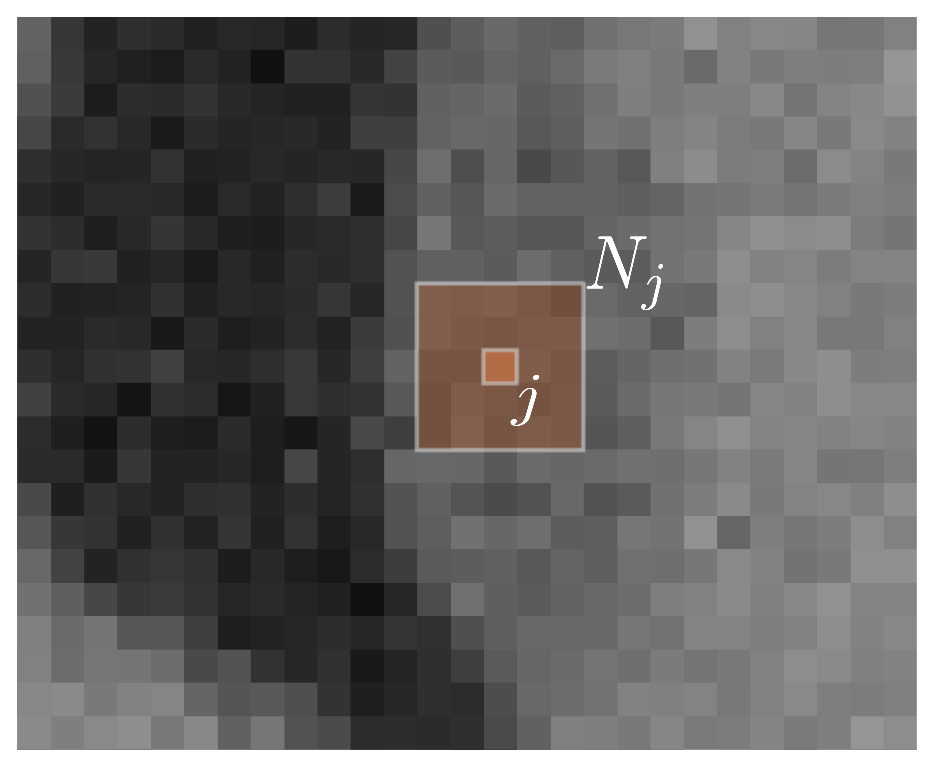
\includegraphics[height=55mm]{eps/chapitre3/Mean_Filter.eps}}
\subfigure[]{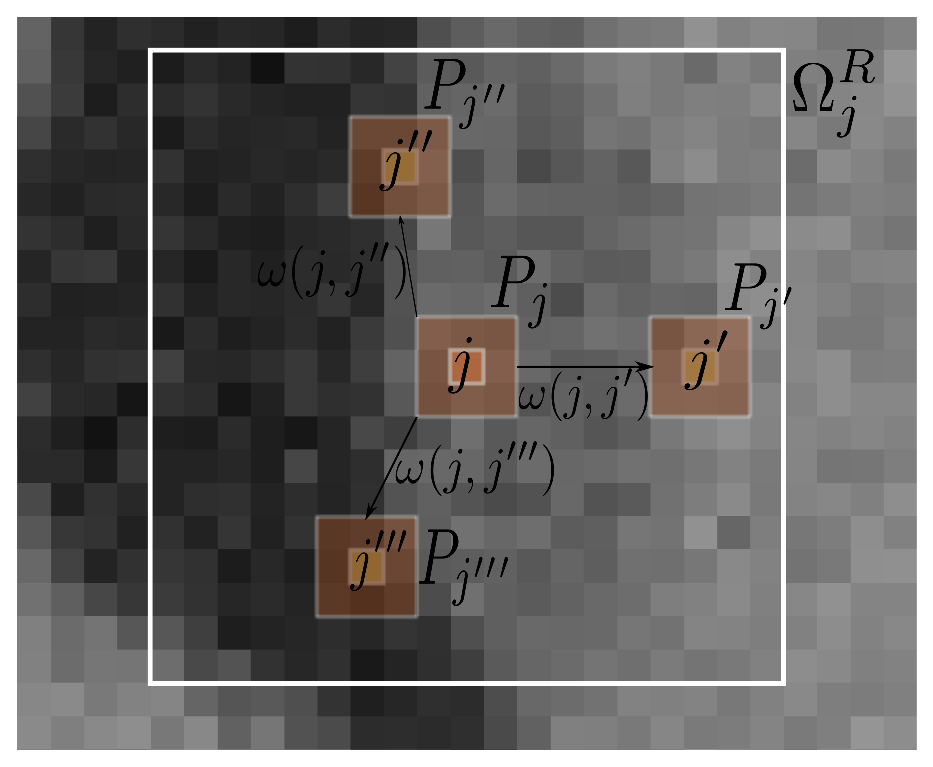
\includegraphics[height=55mm]{eps/chapitre3/NL_Mean_Filter.eps}}
\end{center}
\caption[Comparaison entre un d�bruitage par moyennes et par moyennes non-locales]{\emph{(a) D�bruitage par moyennes. L'estimation de l'intensit� du voxel central est une moyenne de l'ensemble des voxels du voisinage $N_j$. (b) D�bruitage par moyennes non-locales~\cite{Buades:MMS:2005}. Un poids est attribu� � chaque voxel de la zone de recherche $\Omega^R_j$ selon la similarit� de son patch avec celui du voxel central.}}
\label{fig:mean_filter}
\end{figure}

Telle qu'elles sont d�finies, les moyennes non-locales ont montr�s une grande efficacit� dans le d�bruitage de zones r�guli�res mais aussi dans des zones textur�es~\cite{Salmon:2010}, ce qui est peu �tonnant vu que certains travaux pr�liminaires ayant men� � cette approche ont �t� fait dans le cadre de la synth�se de textures~\cite{Criminisi:CVPR:2003}.
% 

% A rajouter dans l'�tat de l'art : \cite{VanDeVille:TIP:2011}.

\subsection{Interpr�tation des moyennes non-locales}

Plusieurs points de vue peuvent �tre adopt�s pour l'interpr�tation des moyennes-non-locales.
Un premier lien a �t� �tabli avec les variations totales, o� le d�bruitage d'une image consiste en la minimisation d'une fonctionnelle constitu�e de la somme d'un terme d'attache aux donn�es (diff�rence entre l'image estim�e et l'image originale) et d'un terme de r�gularisation, p�nalisant le bruit � haute-fr�quence.
Des termes non-locaux sont introduits dans cette fonctionnelle afin de favoriser les similarit� de l'image \cite{Kindermann:MMS:2005, Gilboa:MMS:2008, Azzabou:CVPR:2007}.
Dans ce cadre, les moyennes non-locales sont vu comme une �tape d'une descente de gradient pour la minimisation de la fonctionelle .

Les moyennes non-locales ont �galement �t� �tudi�es directement depuis l'espace des patches.
Les travaux de \cite{Tschumperle:ICIP:2009} les interpr�tent comme une �tape d'une �quation de chaleur dans l'espace des patches et �tablissent des liens avec les algorithmes classiques de diffusion.
Ce point de vue est soutenu par l'article de \cite{Peyre:CVIU:2009} qui consid�re qu'une image repose sur une vari�t� dans l'espace des patches, les moyennes non-locales consistant en une diffusion dans cette vari�t�.
Enfin, un lien avec les �quations de Fokker-Planck est mis en �vidence par \cite{Singer:SIAMJIS:2009}, rapprochant les moyennes non-locales des processus de Markov.

D'autres auteurs adoptent un point de vue statistiques pour interpr�ter les moyennes non-locales.
Par exemple, \cite{Goossens:LNLA:2008} d�montre un lien avec les estimateurs robustes (ou plut�t, la premi�re it�ration d'un algorithme d'optimisation) et pose la question de l'utilisation du noyau gaussien si le bruit ne l'est pas.
Par ailleurs, \cite{Deledalle:TIP:2009} propose un algorithme it�ratif fond� sur l'estimation du maximum de vraisemblance permettant de prendre en compte diff�rents types de bruit.
Enfin, \cite{Salmon:ICIP:2009} consid�re les moyennes non-locales comme une agr�gation bay�sienne d'estimateurs en chaque patches.
L'article de \cite{Katkovnik:IJCV:2010} assimile quant � lui la premi�re version des moyennes non-locales � une r�gression lin�aire d'ordre $0$ et l'�tend � des niveaux sup�rieurs.

De plus, certains travaux ont permis d'�tablir un lien entre le filtre non-local et les diff�rents filtres d�j� existants (tel que le filtre bilat�ral, les filtres bay�siens,\ldots).
Des techniques de r�gularisation de graphes discr�tes, (voir les travaux de \cite{Bougleux:IJCV:2009} et \cite{Elmoataz:TIP:2008}) permettent de faire le lien entre ces diff�rentes techniques.
Ces m�thodes de r�gularisation peuvent �tre vues comme des versions discr�tes d'un formalisme plus g�n�ral appell� \emph{Non local data and smoothness term (NDS)} \cite{Mrazek:2006}. 
Ce formalisme d�finit une forme g�n�rale permettant l'unification de nombreux filtres existants par la somme d'un terme d'attache aux donn�es et d'un terme de lissage.
Il est �tendu � la prise en compte des patches par l'article de \cite{Pizarro:IJCV:2010}, d�finissant ainsi le \emph{Generalized NDS (GNDS)}, dont le NDS est un cas particulier.


\subsection{Limites de l'approche non-locale et influence de ses param�tres}

Les deux inovations permettant une grande efficacit� de ce filtre sont la non-localit� et l'utilisation de patches.
Deux hypoth�ses importantes~\cite{Szlam:UCLA:2008} sont ainsi faites concernant l'image trait�e : 
\begin{enumerate}
        \item il existe des patches similaires dans l'image (hypoth�se de redondance de l'information),
        \item des patches similaires ont des voxels centraux similaires.
\end{enumerate}

Il est cependant d�montr� \cite{Duval:2011} que ces hypoth�ses ont plusieurs cons�quences lors du d�bruitage des images : 
\begin{itemize}
 \item le filtre a un impact cons�quent sur des images p�riodiques (par exemple des images alternant des bandes blanches et noires)
 \item la zone de recherche $\Omega^R_j$ a un impact sur la qualit� visuelle du d�bruitage,
 \item un grand patch tend � flouter l'image,
 \item une perte de contraste d�pendant du niveau d'occurence de chaque patch est observ�e,
 \item moins les d�tails sont contrast�s, plus ils sont d�grad�s.
\end{itemize}
Le choix des param�tres se fera donc en tenant compte de ces propri�t�s.

Plusieurs strat�gies ont �t� adopt�es pour calculer de mani�re automatique le param�tre $h$ \cite{Tasdizen:ICIP:2008,Coupe:TMI:2008}. 
L'article de \cite{Buades:MMS:2005} propose de fixer ce param�tre selon la r�gle : $h = 10\sigma$, o� $\sigma$ est l'�cart-type du bruit.
Cependant, les travaux de \cite{Coupe:TMI:2008} proposent une autre m�thode de calcul en montrant que $h$ ne d�pend  pas que de la variance du bruit $\sigma^2$, mais �galement de la taille de la zone de recherche $\lvert \Omega^{R}_{j} \rvert$.
La fen�tre $h$ peut ainsi �tre �valu�e par : $h = 2 \alpha \sigma^{2} \lvert \Omega^{R}_{j} \rvert$ o� seul le param�tre $\alpha$ est � ajuster manuellement.
Dans la cas d'un bruit gaussien, la valeur de $\alpha$ est th�oriquement � $1$ si l'estimation de la variance est correcte.
Un dernier exemple d'ajustement est le travail de \cite{Tasdizen:TIP:2009} qui r�alise un apprentissage sur diff�rentes images ayant un niveau de bruit connu.
La relation lin�aire entre $h$ et $\sigma$ est mise en �vidence et ses param�tres calcul�s en fonction du niveau de bruit et du param�tre $h$ permettant un d�bruitage optimal.

La zone de recherche $\Omega^R_j$ a �t� introduite d'abord dans un soucis d'am�lioration du temps de calcul. 
Cependant, certains auteurs ont observ� qu'elle avait une influence d�terminante sur la qualit� visuelle du d�bruitage \cite{Kervrann:TIP:2006,Gilboa:MMS:2007}.
En effet, l'utilisation d'une zone de recherche trop grande peut conduire � une baisse des performances alors qu'intuitivement, une zone de recherche de plus en plus grande devrait augmenter le nombre de \og bons \fg{} candidats pour effectuer une estimation fiable de la valeur en chaque voxel. 
En pratique, dans les zones o� la fronti�re entre les objets est bien marqu�e, peu de candidats suppl�mentaires sont ajout�s tandis que de nombreux \og mauvais \fg{} le sont, conduisant finalement � une moins bonne estimation.
Cette zone de recherche est donc � ajuster en fonction de l'image consid�r�e \cite{Salmon:2010}. 
Elle peut �galement �tre d�termin�e localement selon la r�gle de Lepski en fonction du niveau de bruit local, comme dans l'article de \cite{Kervrann:TIP:2006}.

\begin{figure}[!t]
\begin{center}
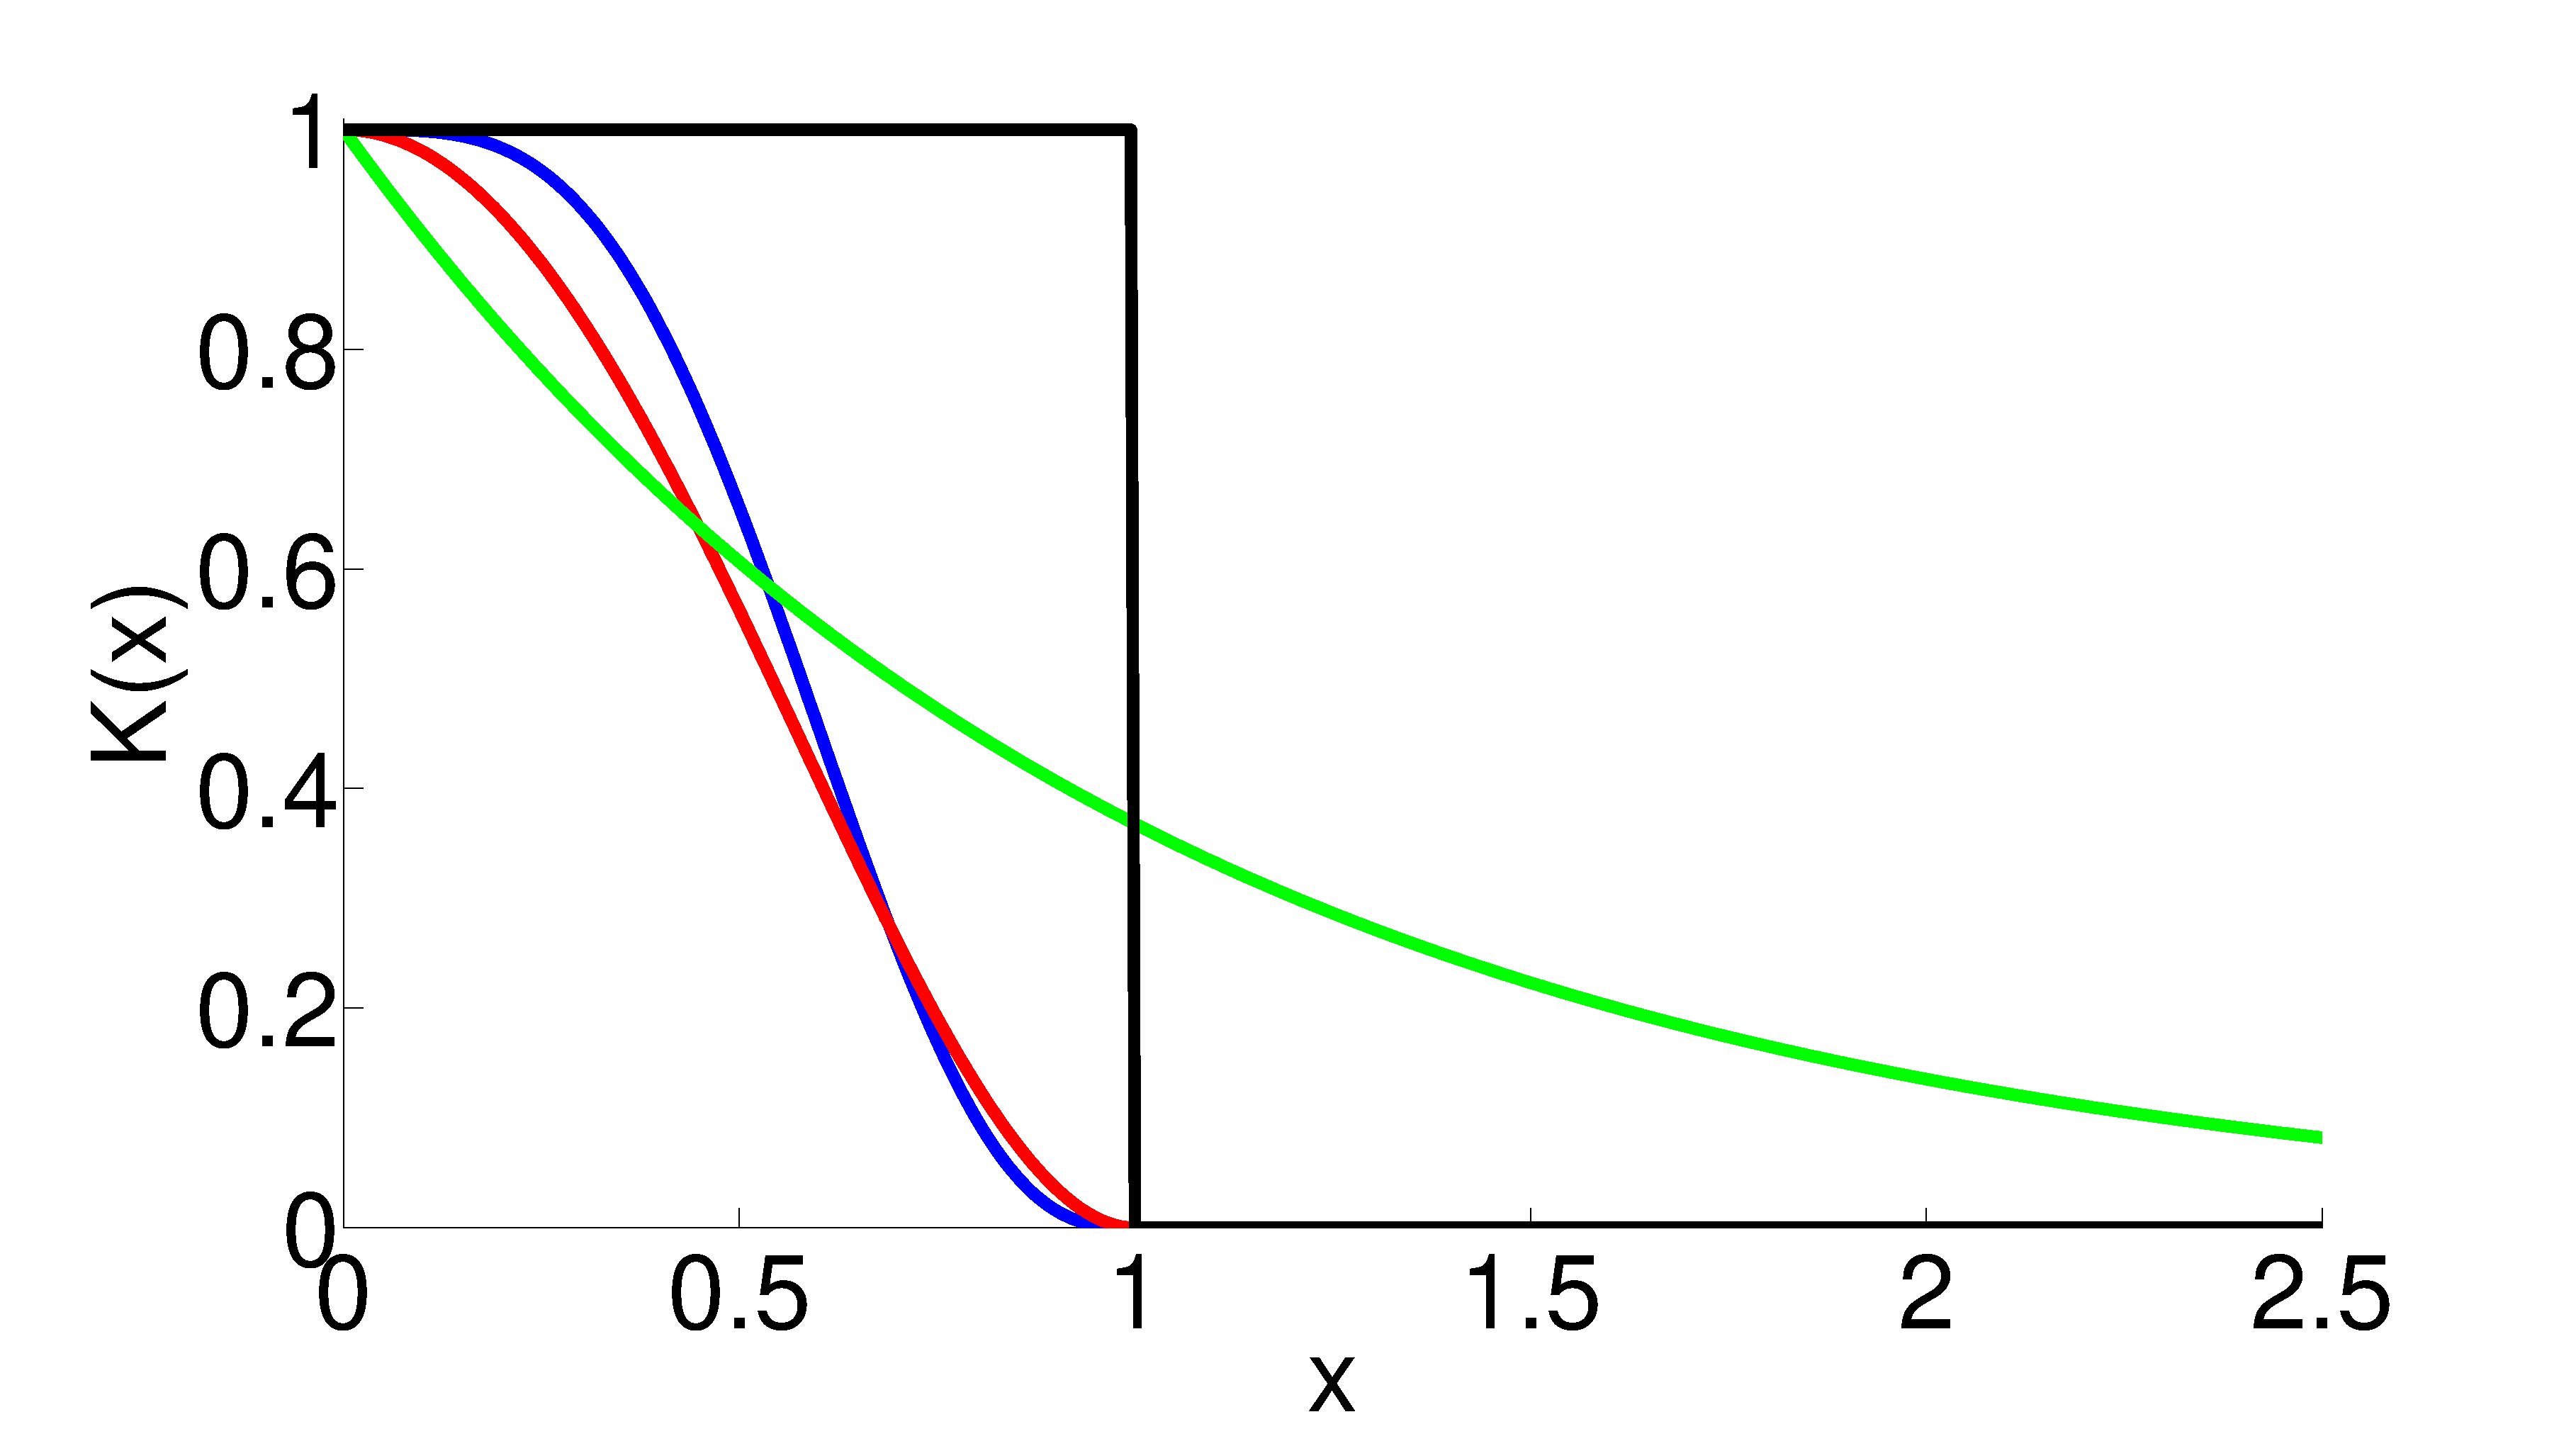
\includegraphics[height=55mm]{eps/chapitre3/kernels.eps}
\end{center}
\caption[Diff�rents noyaux utilis�s dans le cadre des moyennes non-locales]{\emph{Diff�rents noyaux utilis�s dans le cadre des moyennes non-locales. Noir : noyau plat. Vert : noyau gaussien $K(x) = \exp{(-x^2)}$. Rouge : noyau compact polynomial de degr� 4. Bleu : noyau compact polynomial de degr� 6.}}
\label{fig:nlm:kernels}
\end{figure}

D'autres articles ont �tudi� l'impact de la fonction noyau sur le d�bruitage. 
L'article de Buades \cite{Buades:MMS:2005} utilise un noyau de type gaussien $K(x) = e^{-x^2}$, qui est encore largement utilis� dans la litt�rature.
Cependant, des travaux r�cents \cite{Goossens:LNLA:2008, Salmon:2010} ont montr� qu'un noyau � support compact \cite{Remaki:TIP:2000} est pr�f�rable.
En effet, le noyau gaussien a l'inconv�nient de donner une valeur proche de z�ro, mais non nulle, aux patches peu similaires � celui entourant le voxel central, ce qui tend � diminuer l'efficacit� du d�bruitage. 
Certains travaux tronquent le noyau gaussien pour �viter ce probl�me et pour acc�l�rer les traitements \cite{Coupe:TMI:2008}.
Cependant, l'utilisation de noyaux compacts apporte une r�ponse plus naturelle � ce probl�me en d�finissant l'influence des patches peu similaires au patch central comme nulle, tout en assurant la continuit� de ces fonctionnelles. 
Un noyau plat peut �tre employ� afin de privil�gier la vitesse de calcul (mais n'est pas continu) et on peut trouver des noyaux compacts polynomiaux de degr� $4$ \cite{Goossens:LNLA:2008} ou de degr� $6$ \cite{Duval:2010}.
La figure~\ref{fig:nlm:kernels} illustrent cette probl�matique en comparant diff�rents noyaux et d�montre l'utilit� d'un noyau plat par rapport au noyau gaussien (en ne prenant en compte que les patches \og proches \fg{} du patch central) et par rapport au noyau plat (qui n'est pas une fonction continue et ne pond�re pas les patches).

Le choix de la norme est aussi un �l�ment � prendre en compte.
De mani�re g�n�rale, l'utilisation la norme euclidienne pour le calcul de la similarit� entre deux patches a peu �t� remis en cause \cite{Salmon:2010}.
Cependant, quelques alternatives au calcul direct de la distance entre les patches peuvent �tre not�s.
L'article de \cite{Buades:MMS:2005} inclut �galement une pond�ration en fonction de la distance des voxels par rapport au voxel central.
Cependant, il semble que cette pond�ration ait �t� peu retenue dans les travaux ult�rieurs.
Les travaux de \cite{Azzabou:ICIP:2007} et \cite{Tasdizen:TIP:2009} utilisent un dictionnaire issu de l'image et calcul� par une analyse des composantes principales (ACP) de la matrice de covariance construite � partir de l'ensemble des voisinages de l'image.
La comparaison des patches se fait alors dans l'espace construit � partir des composantes pr�sentant les valeurs propres les plus �lev�es. 
Les r�sultats montrent une nette am�lioration des performances du d�bruitage.

L'influence de la taille des patches a �t� �tudi�e par \cite{Mairal:ECCV:2009}.
Le niveau du bruit est � prendre en compte pour d�terminer la taille et/ou la forme de ce param�tre.
Plus le bruit est important, plus il est n�cessaire d'utiliser des grands patches afin de r�aliser une estimation robuste de la similarit�.
De plus, le bruit peut ne pas �tre uniforme sur l'image et la taille du patch doit donc �tre id�alement d�finie localement.
Enfin, de larges patches sont peu adapt�s dans les zones pr�sentant de fortes variations , ayant pour cons�quence un effacement des d�tails isol�s et la pr�sence d'un halo de bruit autour de ces d�tails � cause de la difficult� de trouver des patches similaires.
La nature de l'image � d�bruiter influe �galement sur l'efficacit� de ce param�tre, qui est donc � fixer en fonction de l'image.
Notons l'article de \cite{Manjon:JMRI:2010} introduisant des patches adaptatifs de mani�re � d�bruiter une IRM pr�sentant un bruit variable.
L'article de \cite{Kervrann:IJCV:2008} peut �galement �tre mentionn� pour l'utilisation de cette technique.
Enfin, nous pouvons citer deux techniques utilisant la m�thode SURE (\emph{Stein's unbiased risk estimate}) \cite{Stein:AS:1981} � partir de plusieurs ex�cutions des moyennes non-locales pour estimer l'image d�bruit�e.
La premi�re est celle de \cite{VanDeVille:TIP:2011} qui ex�cute les moyennes non-locales avec plusieurs taille de patches et de zone de recherche, et effectue une combinaison de ces r�sultats afin d'obtenir l'estimation la plus robuste possible en chaque �l�ment de l'image.
Par ailleurs, \cite{Deledalle:JMIV:2011} utilise des patches de formes diverses et agr�ge les diff�rentes estimations localement. 
De plus, ils utilisent une impl�mentation fond�e sur la transform�e de Fourrier rapide de mani�re � acc�l�rer les traitements.
Ses r�sultats montrent une nette diminution du halo de bruit que l'on peut observer avec l'algorithme des moyennes non-locales original.
% Une technique de patches adaptatifs a �t� impl�ment�e par \cite{Kervrann:TIP:2006} dans l'

% D'autres travaux ont cherch� � am�liorer ce filtre. 
% Certains ont acc�l�r� les traitements en partant du principe qu'un voxel appartient � plusieurs patches diff�rents \cite{Coupe:TMI:2008}, la valeur finale du voxel �tant r�cup�r�e par un moyenne sur l'ensemble des patches.

\subsection{Usage des moyennes non-locales}

Depuis son apparition en 2005, les moyennes non-locales ont �t� utilis�es dans d'autres domaines que le d�bruitage d'images.
Le domaine des probl�mes inverses, par la n�cessit� d'une r�gularisation dans le cas de probl�mes mal pos�s, a b�n�fici� de l'apport des moyennes non-locales.
Nous pouvons citer les travaux de \cite{Bougleux:ECCV:2008} sur cette th�matique, ainsi que ceux de \cite{Mignotte:PRL:2008} en d�convolution et ceux de \cite{Rousseau:MIA:2010} en reconstruction de volumes 3D.
En d�convolution, les moyennes non-locales sont utilis�es de mani�re � favoriser les images pr�sentant un haut niveau de redondance, soit dans l'id�al des images invariantes au filtre non-local.

Enfin, les moyennes non-locales ont �galement �t� appliqu� � la segmentation d'images.
Les travaux de \cite{Gilboa:MMS:2008} se sont focalis�s sur la d�finition d'un op�rateur gradient et et d'un op�rateur divergence non-locaux de mani�re � �tendre les techniques fond�es sur des �quations diff�rentielles partielles (EDP) ou des approches variationnelles.
Les travaux de \cite{Bresson:2008} ont d�fini plusieurs fonctionnelles non-locales permettant une segmentation non-supervis�e par contours actifs avec une approche variationnelle.
Les moyennes non-locales ont �galement �t� utilis�es en propagation de labels � partir d'une base d'images dont la v�rit� terrain est connue. 
L'article de \cite{Rousseau:TMI:2011} d�crit une m�thodologie cherchant les patches similaires dans une base d'image, apr�s une recalage affine et une �galisation d'histogramme.
Cette m�thododologie a l'avantage de ne pas n�cessiter de recalage non-lin�aire, et base l'�tape de fusion des labels sur les poids non-locaux calcul�s � travers la base.
Les moyennes non-locales ont �galement �t� introduites dans les lignes de niveaux par~\cite{Jung:SSVM:2011} et ont permis la segmentation de structures dont l'intensit� varie de fa�on lisse, ce qui peut se r�v�l� int�r�ssant dans le cas ou un biais est pr�sent.
% Enfin, l'article de \cite{Wang:CMIG:2008} d�finit une premi�re approche permettant de prendre en compte l'information non-locale dans FCM. 
% Elle est d�crite � la section suivante.


% \subsection{Segmentation non-locale}

Une premi�re utilisation des moyennes non-locales dans l'algorithme FCM a �t� d�finie par~\cite{Wang:CMIG:2008} avec une application � la segmentation c�r�brale.
Cette m�thodologie a �t� d�velopp�e de mani�re ind�pendante de la notre.
Les auteurs utilisent une pond�ration entre information locale et information non-locale en red�finissant la distance entre l'intensit� d'un voxel et le centro�de d'une classe de la fa�on suivante :
\begin{equation}
D^{2}(\mathbf{y}_{j}, \mathbf{v}_{k}) = (1-\lambda_{j}) d^{2}_{l}(\mathbf{y}_{j}, \mathbf{v}_{k}) + \lambda_{j} d^{2}_{nl}(\mathbf{y}_{j}, \mathbf{v}_{k}) \label{nlfcm:wang:distance},
\end{equation}
o� $D(\mathbf{y}_{j}, \mathbf{v}_{k})$ repr�sente la distance entre l'intensit� $\mathbf{y}_{j}$ du voxel $j$ et le centro�de $\mathbf{v}_k$ de la classe $k$.
Cette distance est une combinaison entre une distance locale $d_{l}(\mathbf{y}_{j}, \mathbf{v}_{k})$ et une distance non-locale $d_{nl}(\mathbf{y}_{j}, \mathbf{v}_{k})$.
Le param�tre $\lambda_{j}$ contr�le localement la proportion entre ces deux distances pour le calcul de la distance $D$.

La distance locale est calcul�e de la fa�on suivante :
\begin{equation}
d^{2}_{l}(\mathbf{y}_{j}, \mathbf{v}_{k}) = \frac{\sum_{l \in N{j}} \omega_{l} (\mathbf{y}_{j}, \mathbf{y}_{l}) \lVert \mathbf{y}_{l} - \mathbf{v}_{k} \rVert^{2}_{2}}{\sum_{l \in N{j}} \omega_{l} (\mathbf{y}_{j}, \mathbf{y}_{l})} \label{nlfcm:wang:distance:locale},
\end{equation}
o� $N_{j}$ est un voisinage centr� autour du voxel $j$, $\omega_{l} (\mathbf{y}_{j}, \mathbf{y}_{l}) = e^{-\frac{\lvert \mathbf{y}_{j} - \mathbf{y}_{l} \rvert}{\sigma^{2}}}$ est le poids local accord� au voxel $l$ et $\sigma^{2}$ est la variance sur $N_{j}$.
Cette distance locale repr�sente donc une moyenne pond�r�e sur le voisinage $N_j$, les pond�rations �tant calcul�es � partir de la similarit� entre le voxel central et ses voisins (similarit� voxel � voxel et non similarit� des patches).

La distance non-locale est calcul�e de la fa�on suivante : 
\begin{equation}
d^{2}_{nl}(\mathbf{y}_{j}, \mathbf{v}_{k}) = \sum_{j' = 1}^{N}\omega_{nl}(j,j') \lVert \mathbf{y}_{j'} - \mathbf{v}_{k} \rVert^{2}_{2},
\end{equation}
o� $\omega_{nl}(j,j')$ repr�sente le poids non-local entre les voxels $j$ et $j'$.

% En pratique, ce calcul de la distance non-locale est limit� � une zone de recherche $\Omega^{R}_{j}$ centr�e autour du voxel $j$.
Le param�tre $\lambda_{j}$ est calcul� automatiquement en tenant compte de la similarit� globale du patch $P^{I}_{j}$ au sein de $\Omega^{R}_{j}$. 
Plus il y a de voxels similaires au voxel central au sein de la zone de recherche $\Omega^R_j$, plus le poids de la distance non-locale dans le calcul de la distance g�n�rale sera important.
L'id�e sous-jacente est qu'il existe des parties de l'image pr�sentant peu de similarit�e entre les voxels (par exemple, dans une IRM c�r�brale, autour des sillons c�r�braux) o� il est plus efficace de prendre en compte une similarit� entre les voxels directement plut�t qu'entre les patches.

% Nous montrerons que la correction du bruit pr�sent dans une image ne n�cessite pas de d�finir une telle distance, mais qu'il suffit d'incorporer les moyennes non-locales au sein du terme de r�gularisation de FCM pour obtenir une correction efficace.

\section{C-moyennes floues non-local}
\label{sec:nlfcm}

Nous pr�sentons dans cette section une extension de l'algorithme FCM incluant les moyennes non-locales au sein du terme d'attache aux donn�es de mani�re � am�liorer la prise en compte du biais en intensit� et au sein du terme de r�gularisation de mani�re � am�liorer celle du bruit.
% Dans la suite du manuscrit, l'impl�mentation des moyennes non-locales utilise un noyau de type gaussien $K(x) = e^{\frac{-x}{h}}$ et la norme euclidienne pour le calcul des similarit�s. 
% L'estimation de la fen�tre $h$ est inspir� de \cite{Coupe:TMI:2008}, laissant un param�tre $\alpha$ � �valuer.

\subsection{Terme d'attache aux donn�es}
\label{subsec:nl:dd}

Comme pr�cis� dans la section \ref{subsec:fcm:def}, l'algorithme FCM consid�re que les centro�des des classes sont invariants au sein de l'espace de l'image, le rendant sensible � l'inhomog�n�it� des intensit�s.
Nous avons vu � la section~\ref{subsec:fcm:bias} qu'il est alors n�cessaire de d�finir un mod�le du biais explicite de mani�re � en pr�venir les effets sur la segmentation.
Cependant, de nombreuses hypoth�ses doivent �tre faites pour pouvoir estimer ce biais, notamment sur sa nature multiplicative, la nature lente des variations d'intensit� (valable que pour les inhomog�n�it�s dues � l'imageur), la mod�lisation du biais lui m�me (polynomiales, B-Splines,\ldots{}) ou encore la d�finition d'un champ de biais unique ou d'un champ par tissu.

\begin{figure}[!t]
\begin{center}
\subfigure[]{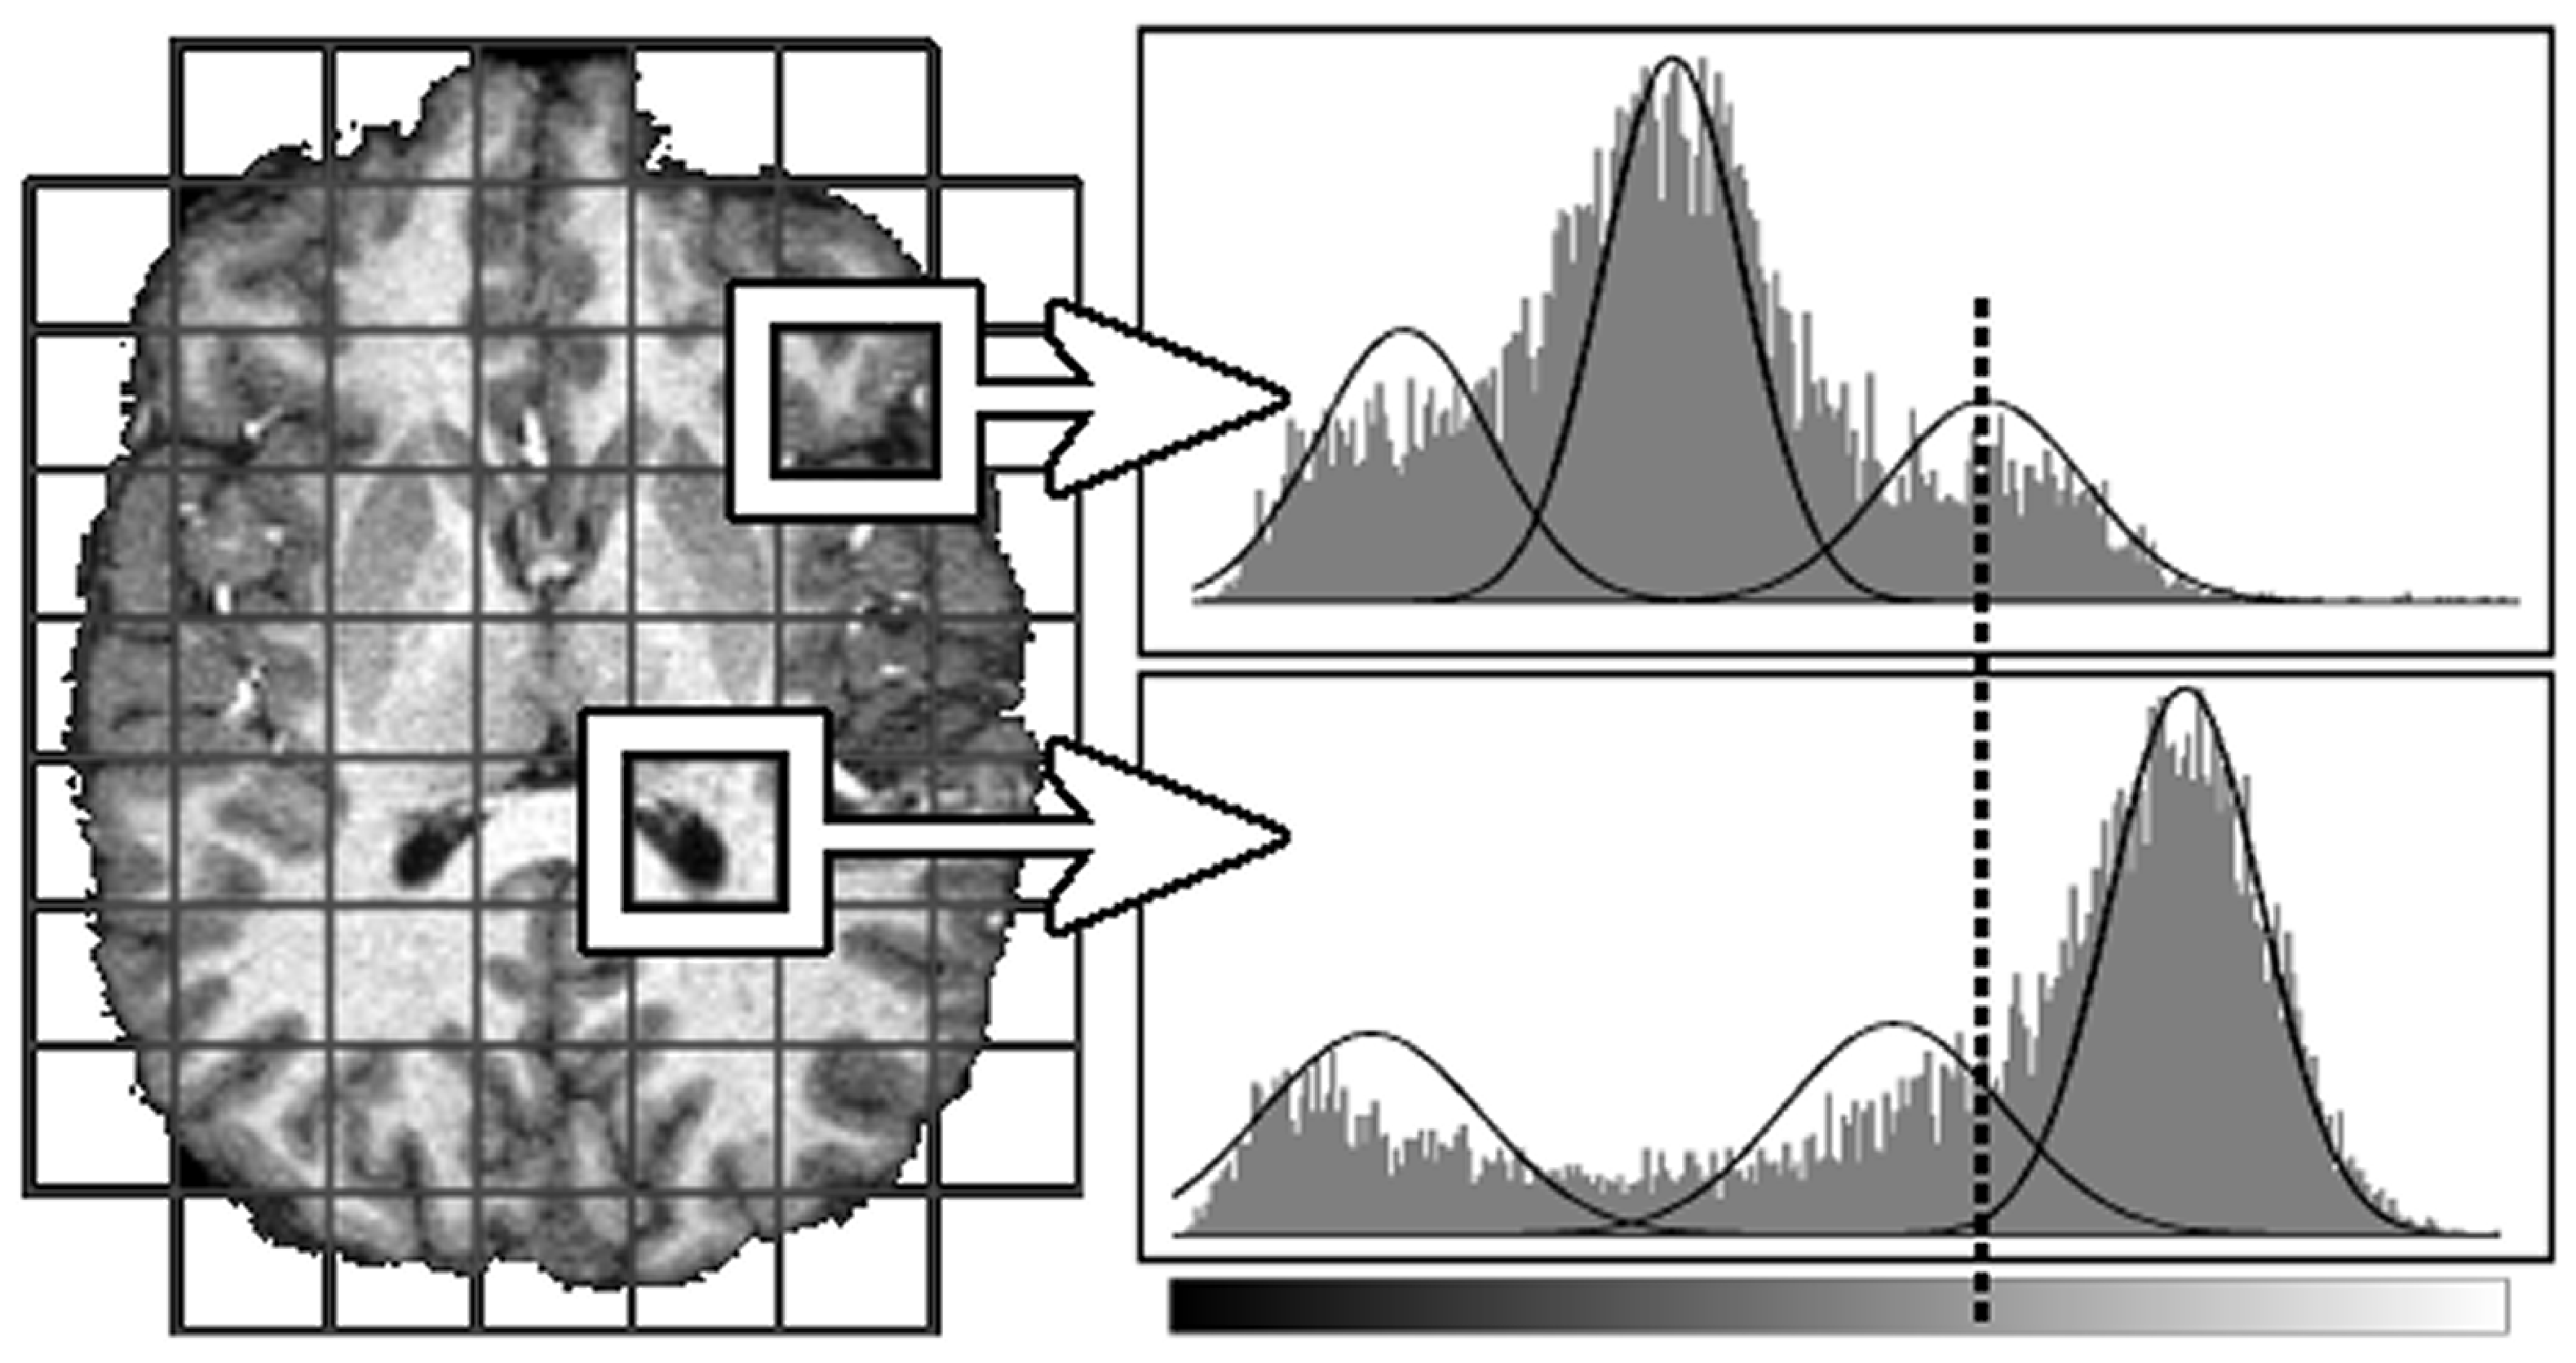
\includegraphics[height=42mm]{eps/chapitre3/BigBox.eps}\label{fig:nlm:seglocale:a}}
\subfigure[]{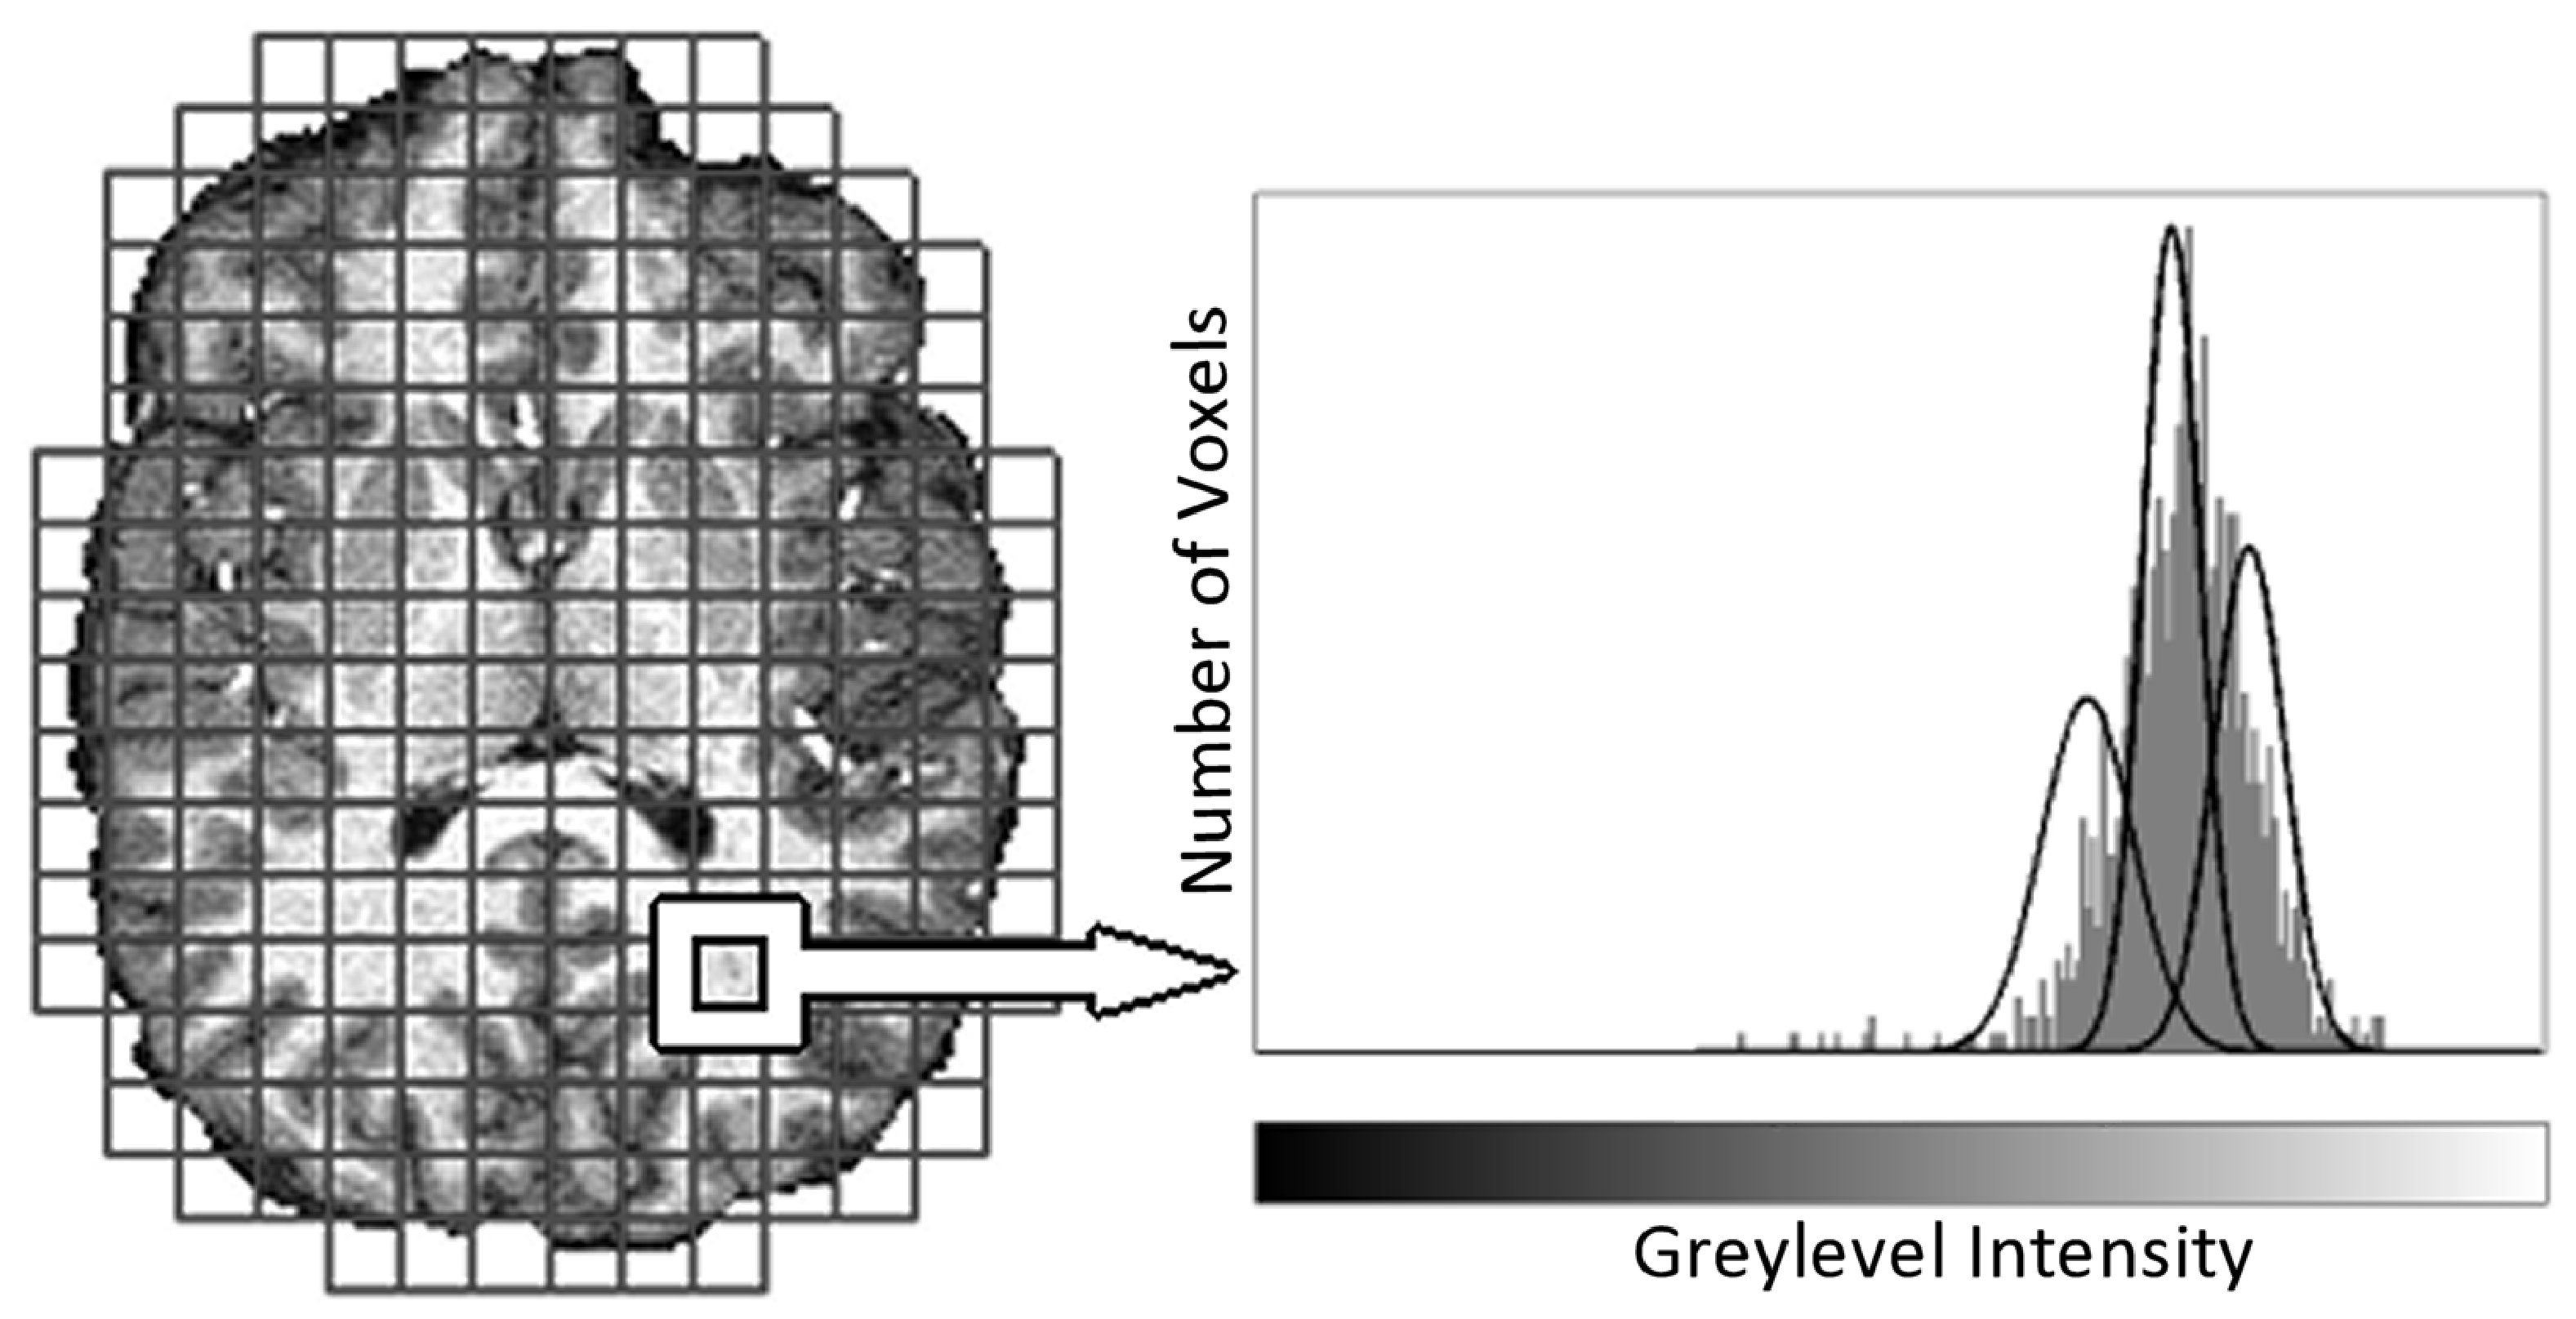
\includegraphics[height=42mm]{eps/chapitre3/LittleBox.eps}\label{fig:nlm:seglocale:b}}
\end{center}
\caption[Mod�lisation locale pour la segmentation]{\emph{Mod�lisation locale de l'image. (a) Deux sous-volumes distincts pr�sentent deux histogrammes diff�rents conduisant � classer une m�me intensit� (marqu�e par la barre verticale) dans deux classes diff�rentes. (b) Illustration de la mauvaise estimation issue de la d�finition de sous-volumes trop petits. Images issues de~\cite{Scherrer:2008}}}
\label{fig:nlm:seglocale}
\end{figure}

Une approche locale de la segmentation est une alternative � explorer car elle permet une estimation des mod�les d'intensit� dans des sous-volumes du volume complet sans avoir recours � une estimation explicite du biais, �vitant de poser les nombreuses hypoth�ses cit�es pr�c�demment.
Une m�me intensit� peut donc �tre �tiquett�e diff�remment selon l'estimation locale du mod�le (voir en Figure~\ref{fig:nlm:seglocale:a}).
La taille des sous-volumes est cependant cruciale car un sous-volume trop important sera sensible � l'inhomog�n�it� tandis qu'un volume trop r�duit risque de conduire � une mauvaise �valuation du mod�le d'intensit� local (voir en Figure~\ref{fig:nlm:seglocale:b}). 
Dans le cas de l'IRM c�r�brale, une fen�tre trop petite peut, par exemple, conduire � une mauvaise �valuation dans des zones de grande concentration de mati�re blanche.
En effet, trop peu de voxels repr�sentant la mati�re grise ou le LCR (voir aucun) seraient alors pris en compte pour permettre une estimation fiable des centro�des des classes repr�sentant ces tissus. 
Or l'algorithme FCM reposant sur l'estimation de ces centro�des, cela conduirait � une classification finale fauss�e.

D�finie dans le cadre de FCM, cette notion de mod�le local se traduit par la minimisation de la fonction d'�nergie suivante : 
\begin{equation}
J = \sum_{j \in \Omega} \sum_{k=1}^{C} u^{q}_{jk} \lVert \mathbf{y}_{j} - \mathbf{v}_{jk} \rVert_{2}^{2}. \label{eq:fcm:local}
\end{equation}
La diff�rence entre cette fonction co�t et celle de l'algorithme FCM classique r�side dans l'introduction de centro�des locaux $\mathbf{v}_{jk}$ fournissant une �valuation du mod�le d'intensit� au voxel $j$.
Des approches par recouvrement de sous-volumes ont �t� d�finies comme celle de \cite{Zhu:NeuroImage:2003} comportant une �tape de classification par FCM proprement dite, puis une �tape de fusion de l'information.
De m�me, \cite{Scherrer:TMI:2009} introduit des mod�les markoviens locaux par la division de l'image en sous-volumes et estime ces mod�les en coop�ration avec les mod�les voisins afin d'assurer la coh�rence de l'ensemble de la segmentation.
Cependant, ces deux approches peuvent �tre consid�r�es comme un d�placement du probl�me de l'�valuation d'un mod�le global vers celui de la fusion de plusieurs sous-mod�les.

A notre connaissance, aucune m�thode ne permet la prise en compte des mod�les voisins sans cette �tape de fusion.
Cependant, l'approche non-locale permet de mettre en \oe uvre une pond�ration entre les diff�rents voxels de l'image en fonction de la similarit� de leur patch.
En faisant l'hypoth�se que deux voxels dont les patches sont similaires font partie du m�me tissu, il est possible d'utiliser ces pond�rations pour prendre en compte les mod�les voisins (c'est-�-dire l'estimation des centro�des locaux aux voxels voisins) pour diminuer le risque qu'entra�ne une mauvaise �valuation des centro�des locaux.
Un terme d'attache aux donn�es non-local est alors d�fini de la fa�on suivante :
\begin{equation}
J_{NL-FCM} = \sum_{j \in \Omega} \sum_{k=1}^{C} u_{jk}^{q} \sum_{l \in \Omega^{R_d}_{j}} \omega_{nl}(j, l) \Vert \mathbf{y}_{j} - \mathbf{v}_{lk} \Vert_2^{2} \label{eq:nlfcm:dd}.
\end{equation}
Le terme $\omega_{nl}(j, l)$ est calcul� selon l'�quation \ref{nlfcm:poids:definition} et $h$ selon la m�thode d�finie par \cite{Coupe:TMI:2008}.
% Ce terme d'attache aux donn�es permet une meilleure robustesse de la segmentation en cas de mauvaise �valuation de certains mod�les locaux.

Deux diff�rences sont notables par rapport � la d�finition standard de FCM (donn�e par l'�quation \ref{eq:fcm}).
La premi�re a d�j� �t� �voqu�e et consiste � remplacer le terme global des centro�des $\mathbf{v}_{k}$ dans FCM par un terme local $\mathbf{v}_{jk}$ de mani�re � b�n�ficier d'une �valuation locale du mod�le d'intensit�.
Ces centro�des locaux sont calcul�s � partir d'un sous-volume $M_j$ centr� autour du voxel $j$ et dont l'influence de la taille est discut�e plus loin.
La deuxi�me diff�rence est que chaque mod�le inclus dans la zone de recherche $\Omega^{R_d}_{j}$ va avoir une influence sur la classification finale du voxel $j$.
Un mod�le �tant d�fini pour chaque voxel de l'image, cette proportion est donc contr�l�e par le poids non-local $\omega_{nl}(j,j')$ traduisant la similarit� entre le voxel $j$ et chacun des voxels $j'$ inclus dans la zone de recherche.  

\subsection{Terme de r�gularisation}
\label{subsec:nl:reg}

Comme vu dans la section~\ref{subsec:fcm:noise}, le terme de r�gularisation de la fonction d'�nergie de FCM s'apparente la plupart du temps � l'expression d'un filtrage m�dian ou par moyenne pour lisser la segmentation, comme dans l'article de~\cite{Ahmed:TMI:2002}.
L'article de~\cite{Pham:CVIU:2001} a une approche l�g�rement diff�rente �tant donn� que le lissage ne se fait qu'en prenant en compte l'ensemble des classes except�e la classe courante, ce qui permet de favoriser le terme d'attache aux donn�es si la classe courante est bien repr�sent�e dans le voisinage. 
Plusieurs articles ont introduit diff�rentes strat�gies permettant de prendre en compte la similarit� entre les voxels (introduisant ainsi une pond�ration entre les voxels d'un m�me voisinage), mais cette prise en compte n�cessite le calcul de plusieurs variables additionnelles ou la d�finition d'une image interm�diaire (voir la sous-section \ref{subsec:fcm:noise}).

Les moyennes non-locales sont particuli�rement int�ressantes dans cette situation, car elles fournissent les outils n�cessaires � une pond�ration relativement ais�e des voxels d'int�ret au sein de la zone de recherche.
Le r�le de poids non-locaux est donc de s�lectionner les voxels les plus pertinents au sein de la zone de recherche pour effectuer la r�gularisation en fonction de leur degr� de similarit� avec le voxel courant.
L'hypoth�se que nous faisons est que si les patches de deux voxels sont similaires, alors ils appartiennent au m�me tissu.
L'objectif est d'obtenir une r�gularisation plus lisse de fa�on adaptative.

Le terme de r�gularisation d�fini dans cette section s'inspire de celui de \cite{Pham:CVIU:2001} (dont la d�finition est donn�e par l'�quation \ref{eq:rfcm}), calculant la proportion d'une classe au sein d'un voxel en prenant en compte la proportion des autres classes dans le voisinage.
Le terme de r�gularisation non-local est exprim� de la fa�on suivante :
\begin{equation}
J_{NL\textrm{-}Reg} = 
\frac{\beta}{2} \sum_{j \in \Omega} \sum_{k=1}^{C} u_{jk}^{q} \sum_{j' \in \Omega^{R_{r}}_{j}} \omega_{nl}(j, j') \sum_{l \in L_{k}} u_{j'l}^{q} \label{eq:nlfcm:reg}.
\end{equation}

Rappelons que $L_{k}=[\![1,C]\!]\setminus \{k\} = \{1, \ldots, k-1, k+1, \ldots, C\}$ repr�sente l'ensemble des classes except�e la classe dont on effectue la r�gularisation et $\Omega^{R_{r}}_{j}$ repr�sente la zone de recherche centr�e autour du voxel $j$ destin�e � calculer les poids non-locaux pour la r�gularisation.
Le param�tre $\beta$ contr�le les poids respectifs entre le terme de r�gularisation et le terme d'attache aux donn�es au sein de la fonction d'�nergie.
Le terme $\omega_{nl}(j, l)$ est calcul� selon l'�quation \ref{nlfcm:poids:definition} et $h$ selon la m�thode d�finie par \cite{Coupe:TMI:2008}.

\subsection{Algorithme non-local complet}

L'association des deux termes non locaux donne un algorithme de segmentation non local complet permettant de prendre en compte l'inhomog�n�it� en intensit� et le bruit de l'image. 
La fonction d'�nergie devient donc : 
\begin{equation}
\begin{array}{l l}
J_{NL\textrm{-}R\textrm{-}FCM} & = J_{NL\textrm{-}FCM} + J_{NL\textrm{-}Reg} \\
 & = \left\{ 
\begin{array}{c}
\sum_{j \in \Omega} \sum_{k=1}^{C} u_{jk}^{q} \sum_{j' \in \Omega^{R_d}_{j}} \omega_{nl}(j, j') \Vert \mathbf{y}_{j} - \mathbf{v}_{j'k} \Vert_2^{2} + \\
\frac{\beta}{2} \sum_{j \in \Omega} \sum_{k=1}^{C} u_{jk}^{q} \sum_{j'' \in \Omega^{R_{r}}_{j}} \omega_{nl}(j, j'') \sum_{l \in L_{k}} u_{j'l}^{q} \label{eq:nlfcm:reg}.
\end{array}
\right.
\end{array}
\end{equation}
Il est important de noter que les poids $\omega_{nl}(\cdot,\cdot)$ pr�sents dans le terme d'attache aux donn�es et le terme de r�gularisation sont distincts car les zones de recherche $\Omega^{R_d}_{j}$ et $\Omega^{R_r}_{j}$ ne sont pas n�cessairement identiques.
Etant donn� que le biais est un art�fact lisse variant lentement le long de l'image, la zone de recherche $\Omega^{R_d}_{j}$ peut �tre choisi aussi grande que possible.
Par contre, la correction du bruit nous impose un plus petit rayon pour $\Omega^{R_r}_{j}$ afin de limiter la prise en compte de patches peu similaires lors du calcul des poids.

Les diff�rentes �tapes permettant de minimiser la fonction d'�nergie du FCM non-local sont les suivantes : 
\begin{enumerate}
\item Calculer les poids non-locaux $\omega_{nl}$ pour le terme d'attache aux donn�es et le terme de r�gularisation.
\item Calculer les centro�des $\mathbf{v}_{jk}$ pour tout $(j,k) \in [\![ 1,C ]\!]\times \Omega$ selon : 
\begin{equation}
\mathbf{v}_{jk} = \frac{\sum_{l \in M_{j}} u_{lk}^{q} \mathbf{y}_{l}}{\sum_{l \in M_{j}} u_{lk}^{q}}.
\end{equation}
\item Calculer $u_{jk}$ pour tout $(j,k) \in [\![ 1,C ]\!]\times \Omega$ selon : 
\begin{equation}
 u_{jk} = \frac{(\sum_{j' \in \Omega^{R_d}} \omega_{nl}(j, j')\lVert \mathbf{y}_{j} - \mathbf{v}_{k} \rVert^{2} + \beta \sum_{j'' \in \Omega^{R_r}} \omega_{nl}(j, j'') \sum_{m \in M_{k}} u_{j''m}^{q})^{\frac{-1}{q-1}}}{\sum_{k=1}^{C}(\sum_{j' \in \Omega^{R_d}} \omega_{nl}(j, j')\lVert \mathbf{y}_{j} - \mathbf{v}_{k} \rVert^{2} + \beta \sum_{j'' \in \Omega^{R_r}} \omega_{nl}(j, j'') \sum_{m \in M_{k}} u_{j''m}^{q})^{\frac{-1}{q-1}}}
\end{equation}
\item R�p�ter jusqu'� un minimum local de la fonction d'�nergie : 
\begin{itemize}
\item Recalculer $\mathbf{v}_{jk}$ pour tout $(j,k) \in [\![ 1,C ]\!]\times \Omega$.
\item Recalculer $u_{jk}$ pour tout $(j,k) \in [\![ 1,C ]\!]\times \Omega$.
\end{itemize}

\end{enumerate}

La donn�e d'entr�e de l'algorithme est l'image � segmenter (fournissant $\Omega$ et les valeurs $\mathbf{y}$).
Les param�tres d�terminant son comportement sont : $C$ (le nombre de classes), $\beta$ (qui contr�le le rapport entre le terme d'attache aux donn�es et le terme de r�gularisation), la taille de la zone de recherche pour le calcul des poids non-locaux destin�s � la r�gularisation $\Omega^{R_r}_j$, la taille de la zone de recherche pour le calcul des poids non-locaux destin�s au terme d'attache aux donn�es $\Omega^{R_d}_j$, la taille des sous-volumes $M_j$ permettant l'estimation des mod�les locaux et le param�tre de lissage $\alpha$ intervenant dans l'estimation de $h$.
\begin{table}[!t]
\begin{center}

\begin{tabular}{|c|c|}

\hline
NL-FCM & Terme d'attache aux donn�es non-local \\
\hline
NL-Reg & Terme de r�gularisation non-locale \\
\hline
NL-R-FCM & FCM avec attache aux donn�es et r�gularisation non-locals \\
\hline

\end{tabular}
\caption[R�capitulatif des acronymes utilis�s pour FCM non-local]{\emph{R�capitulatif des acronymes utilis�s pour les diff�rentes versions du FCM non-local.}\label{fig:nlfcm:acronymes}}
\end{center}
\end{table}
Le tableau~\ref{fig:nlfcm:acronymes} r�sume l'ensemble des terminologies utilis�es pour d�signer les diff�rentes version de l'algorithme.


\section{Validations}
\label{sec:nlfcm:validations}

Les exp�riences sont men�es tout d'abord sur des images simul�es fournies par la base BrainWeb \cite{Kwann:VBC:1996, Cocosco:NeuroImage:1997}, puis sur des cas r�els fournis par la base IBSR (\emph{Internet Brain Segmentation Repository}).

Consid�rant tout d'abord la base BrainWeb, trois s�ries d'exp�riences sont men�es de mani�re � d�terminer le comportement de l'algorithme FCM non-local :
\begin{enumerate}
        \item �valuation du terme d'attache aux donn�es non-local en utilisant des images ayant 20~\% d'inhomog�n�it� en intensit� (voir la section~\ref{sec:brainweb:nlData}).
        \item \'Evaluation du terme de r�gularisation non-locale en utilisant des images ayant diff�rents niveaux de bruit ricien (voir la section~\ref{sec:brainweb:nlReg}).
        \item �valuation de l'algorithme non-local complet en utilisant des images ayant � la fois 20~\% d'inhomog�n�it� en intensit� et diff�rents niveaux de bruit (voir la section~\ref{sec:brainweb:nlAll}).
\end{enumerate}
Par la suite, l'algorithme FCM non-local complet est appliqu� � l'ensemble de la base IBSR.

L'�valuation des performances des diff�rents algorithmes est faite par comparaison de la segmentation estim�e avec la v�rit� terrain fournie par les bases d'images respectives.
La qualit� de la segmentation est mesur�e par le calcul de l'indice de similarit� Dice : 
$$
Dice = \frac{2\cdotp VP}{2\cdotp VP + FP + FN},
$$
o� $VP$ est le nombre de vrais positifs, $FP$ le nombre de faux positifs et $FN$ le nombre de faux n�gatifs.
Cet indice calcule un taux de recouvrement entre la v�rit� terrain et la segmentation automatique.

De plus, l'�valuation inclut � chaque �tape une comparaison avec d'autres m�thodes de classification reposant sur les champs et cha�nes de Markov.
Ces m�thodes sont : 
\begin{itemize}
        \item SPM5 de Ashburner \emph{et al.}~\cite{Ashburner:NeuroImage:2005},
        \item EMS de Van Leemput \emph{et al.}~\cite{VanLeemput2:TMI:1999},
        \item HMC de Bricq \emph{et al.}~\cite{Bricq:MIA:2008}.
\end{itemize}
Ces trois m�thodes incluent une correction du biais et un terme de r�gularisation markovien.


\subsection{BrainWeb}
\label{subsec:brainweb}

Le site de BrainWeb~\footnote{\url{http://www.bic.mni.mcgill.ca/brainweb/}} permet de simuler des IRM c�r�brales avec diff�rents niveaux de bruit et d'inhomog�n�it� et fournit la v�rit� terrain correspondante, permettant de comparer diff�rents algorithmes de segmentation.
% La connaissance de la v�rit� terrain permet de comparer diff�rents algorithmes de segmentation.
Les images fournies par la base sont issues de 27 acquisitions r�alis�es sur un m�me individu.
Elles sont ensuite moyenn�es pour construire le volume initial auquel sont ensuite appliqu�s divers traitements pour cr�er le fant�me~\cite{Collins:TMI:1998}.
Les images utilis�es sont de taille $181\times181\times217$ avec des voxels isotropes de $1$ mm de c�t�.
Le bruit est de type ricien d'un niveau allant de $0$ � $9$~\% (c'est � dire une amplitude du bruit allant jusqu'� $9$~\% de la valeur maximale de l'image).

\subsubsection{�valuation du terme d'attache aux donn�es}
\label{sec:brainweb:nlData}

L'algorithme est initialis� gr�ce � l'atlas 452 T1 fourni par l'\emph{International Consortium for Brain Mapping} (ICBM).
Il est recal� sur l'image BrainWeb de mani�re lin�aire et affine.
Il permet d'initialiser de mani�re fiable les moyennes locales avant le lancement de NL-FCM proprement dit et fournit une premi�re estimation de la classification des tissus.

\paragraph*{\'Etude des param�tres}

Les param�tres �tudi�s sont la taille de la zone de recherche $\lvert \Omega^{R_{d}}_{j} \rvert$ pour le calcul des poids non-locaux et la taille du voisinage $M_j$ pour le calcul des centro�des locaux.
On pose $n_j$ et $m_j$ tels que $\lvert \Omega^{R_{d}}_{j} \rvert = (2 \cdot n_j + 1)^{3}$ et $\lvert M_{j} \rvert = (2 \cdot m_j + 1)^{3}$.

\begin{figure}[!t]

        \begin{center}
	\subfigure[]{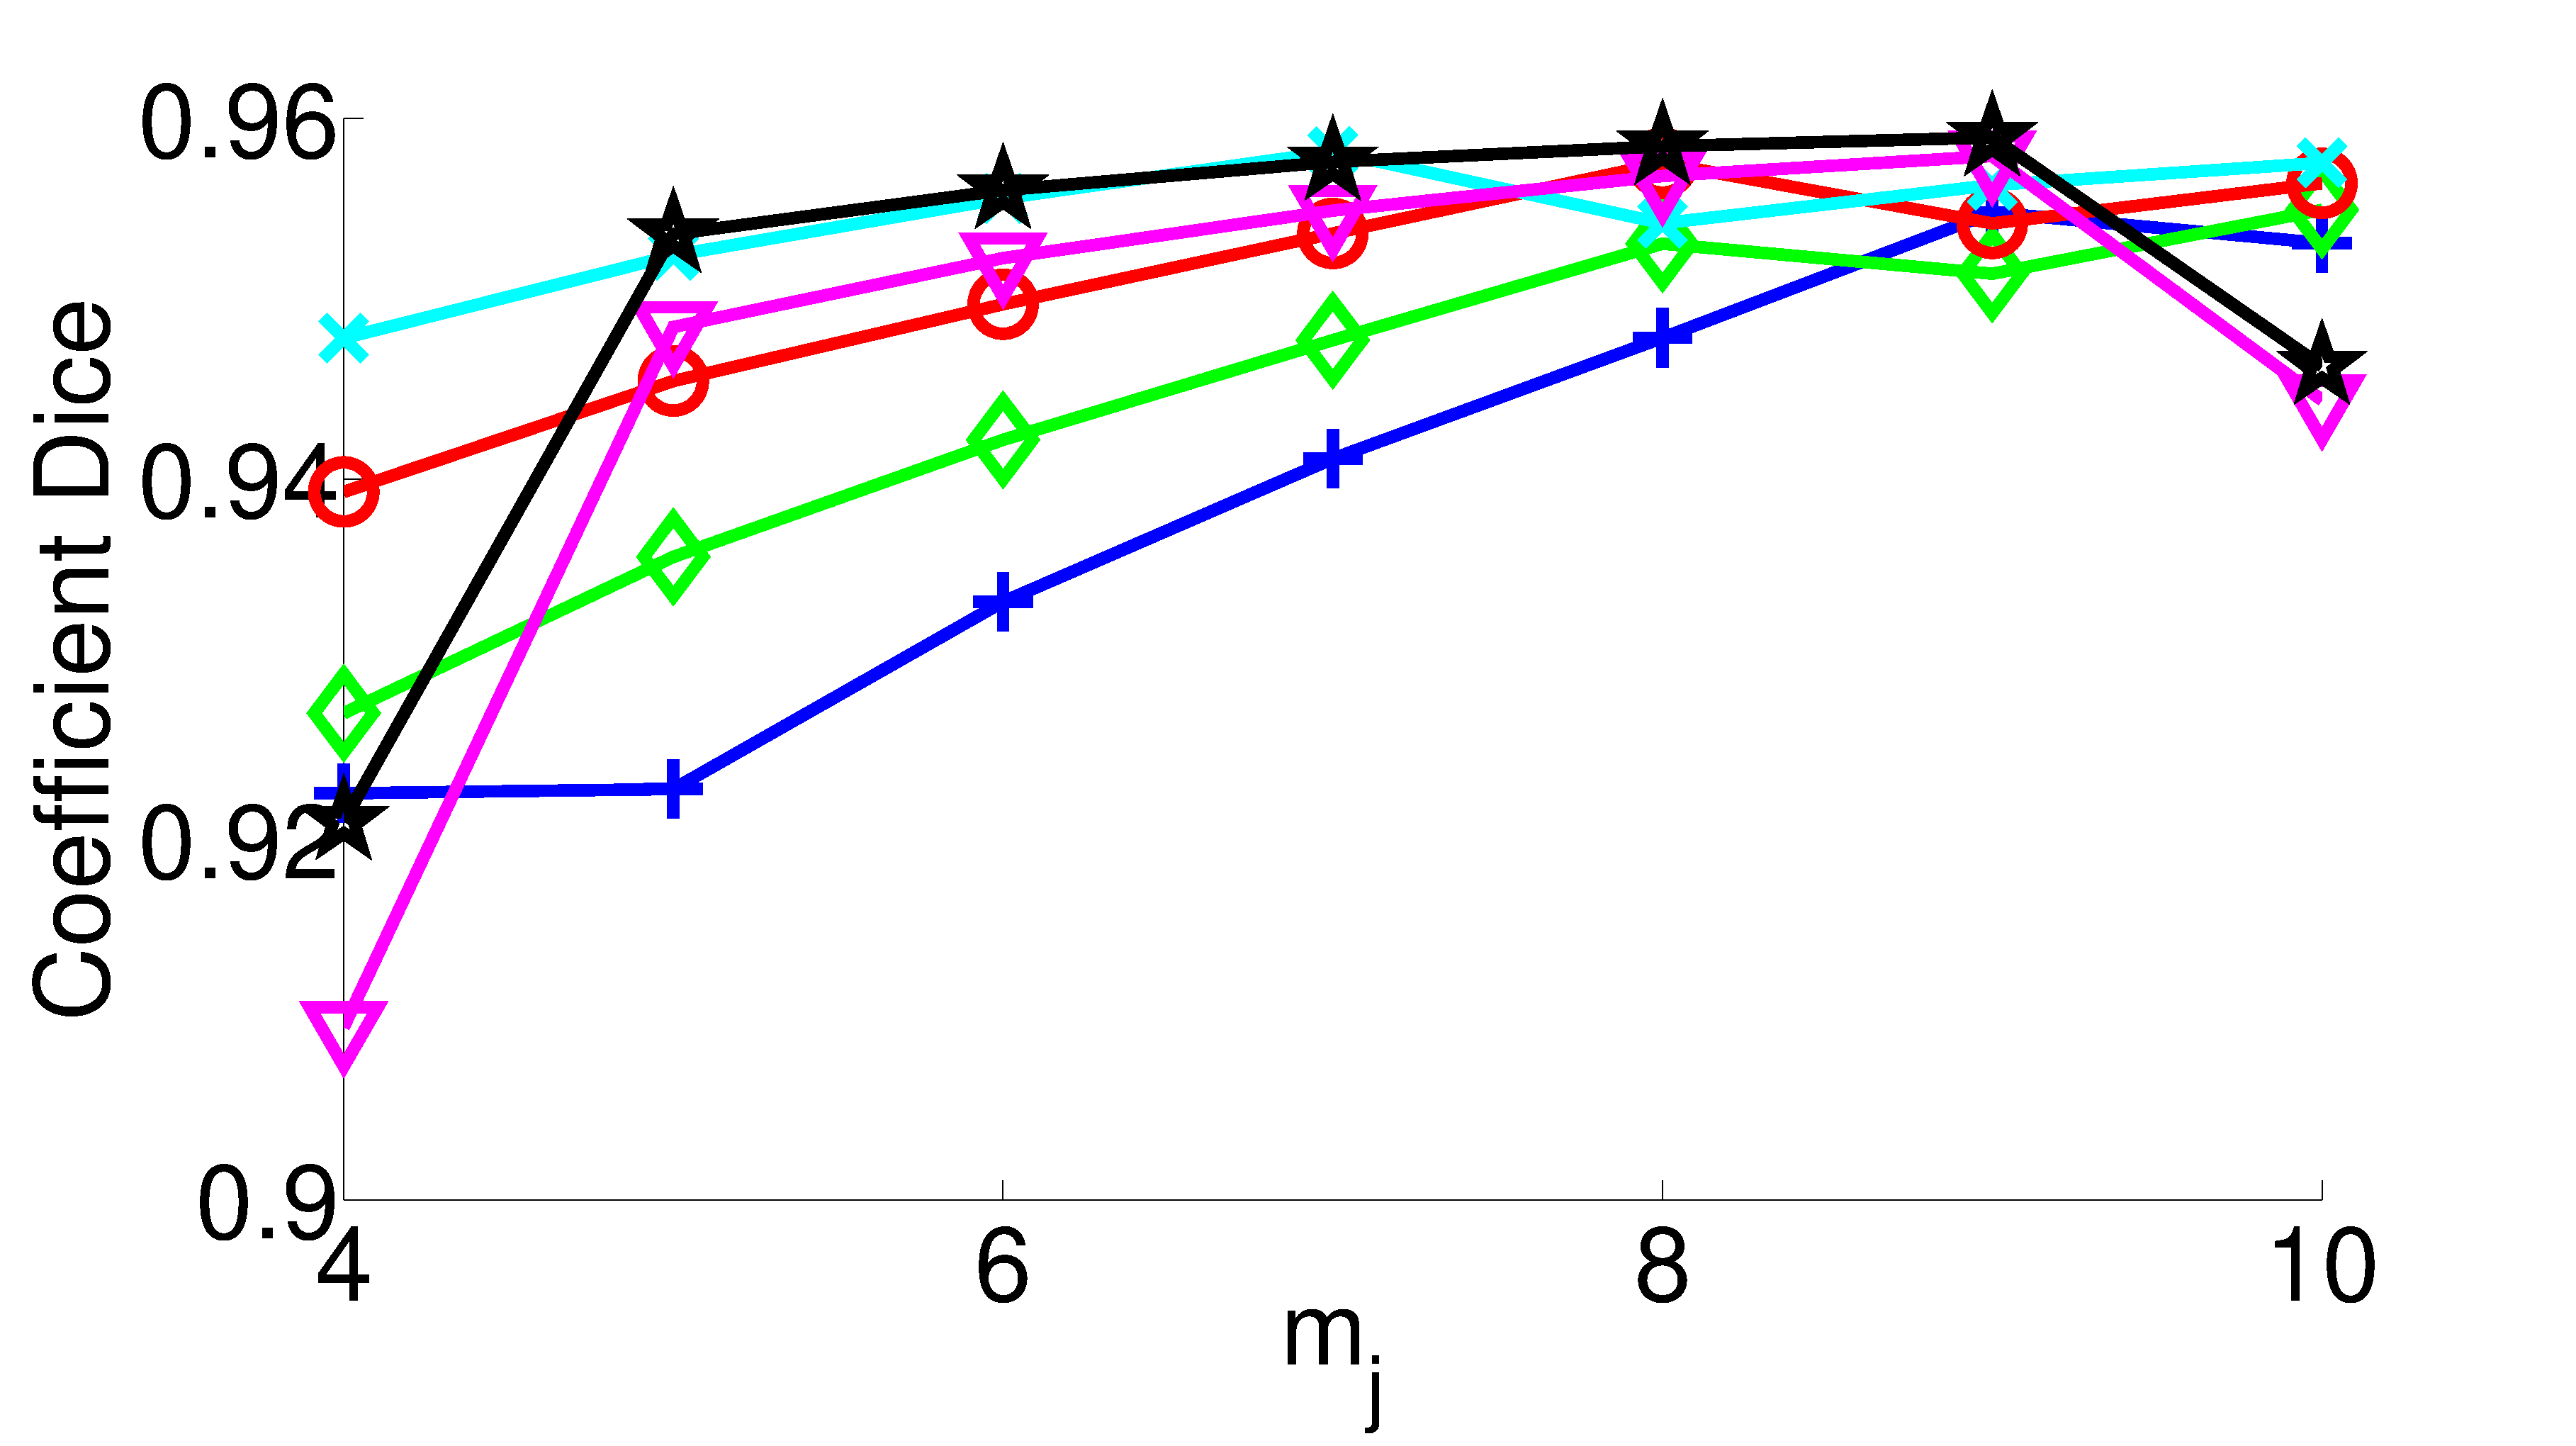
\includegraphics[height=38mm]{eps/chapitre3/Brainweb_Bias_Couple_GM.eps}}
	\subfigure[]{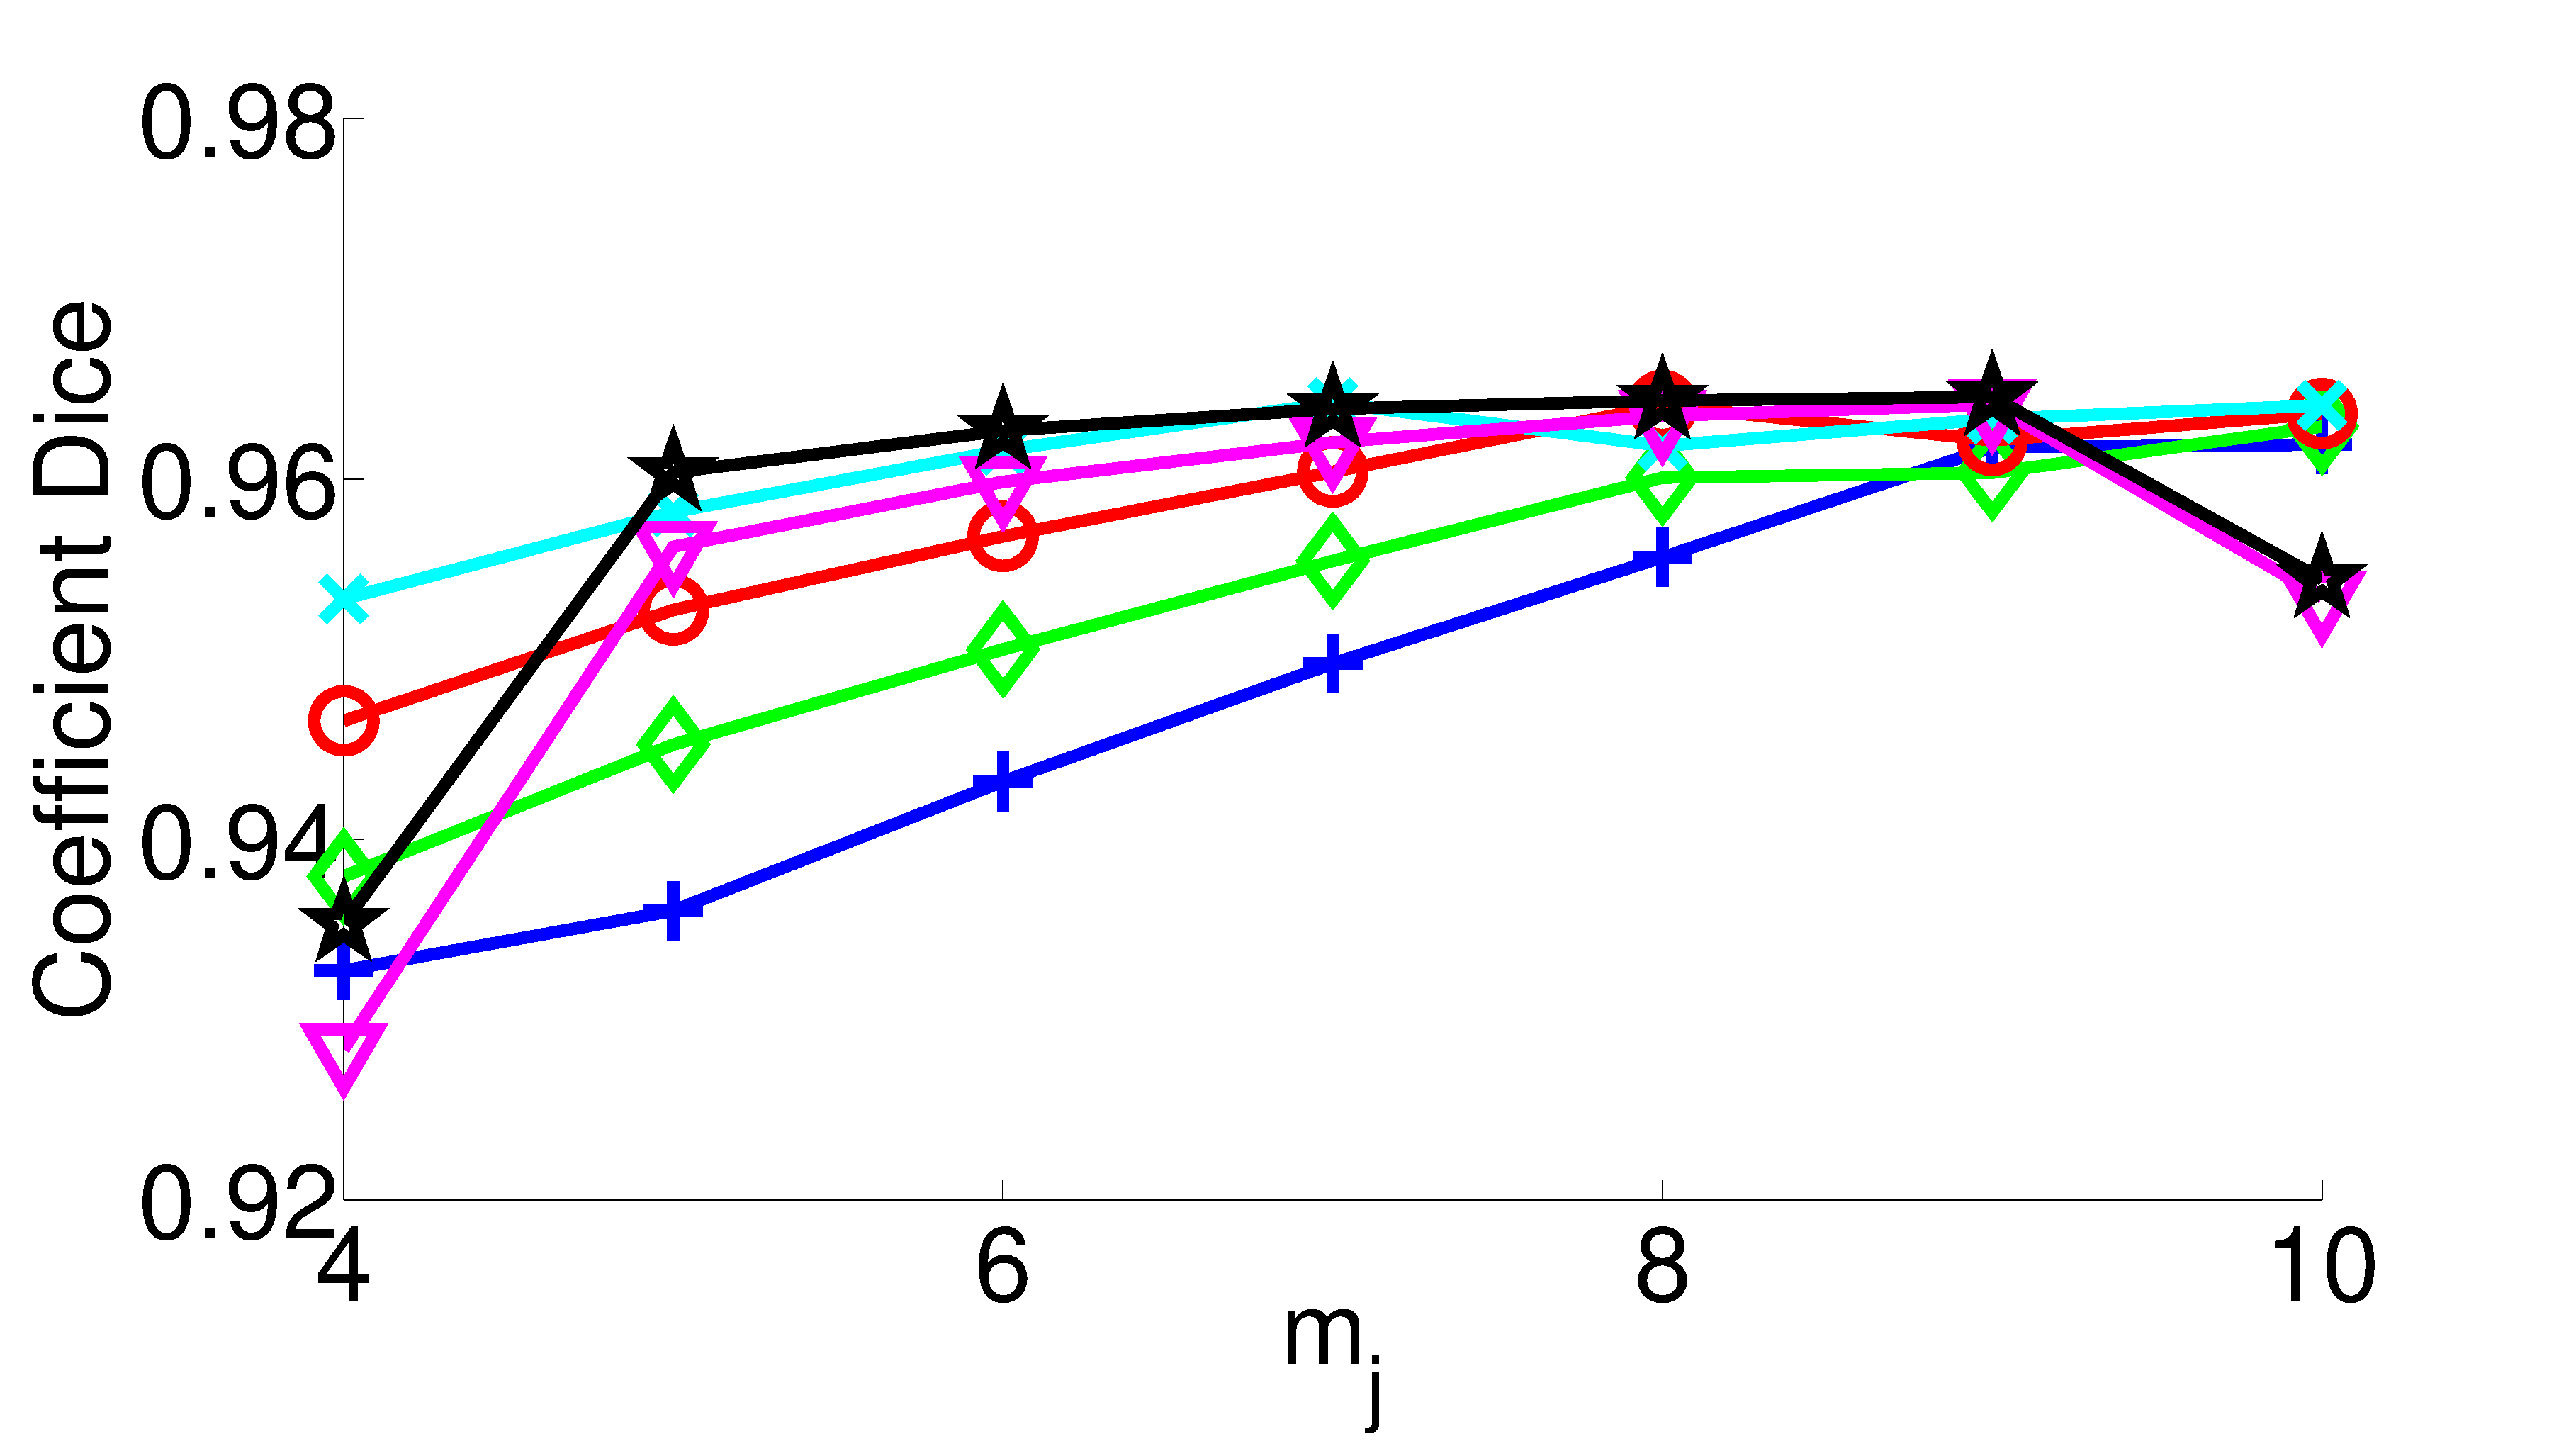
\includegraphics[height=38mm]{eps/chapitre3/Brainweb_Bias_Couple_WM.eps}}
        \end{center}

        \caption[Influence des param�tres $M_j$ et $\Omega^{R_d}_j$ du terme d'attache aux donn�es non-locale]{\emph{Influence des param�tres $M_j$ et $\Omega^{R_d}_j$ du terme d'attache aux donn�es non-locale. L'accroissement de la zone de recherche $\Omega^{R_d}_{j}$ permet de compenser les �ventuelles mauvaises �valuation du mod�le dues � des sous-volumes $M_j$ trop r�duits. (a) Coefficient Dice pour la mati�re grise. (b) Coefficient Dice pour la mati�re blanche. $n_j = 4$ : $+$, $n_j = 5$ : $\diamond$, $n_j = 6$ : $\circ$, $n_j = 7$ : $\times$, $n_j = 8$ : $\bigtriangledown$, $n_j = 9$ : $\star$.}}

        \label{FIG:PARAM:BRAINWEB:BIAS}

\end{figure}

La figure~\ref{FIG:PARAM:BRAINWEB:BIAS} pr�sente les r�sultats avec diff�rents sous-volumes et diff�rentes zones de recherche.
La premi�re partie de la courbe, de $m_j = 5$ � $m_j = 9$, montre comme attendu que pour une m�me valeur de $m_j$, l'accroissement de la taille de zone de recherche permet d'obtenir une meilleure segmentation par la prise en compte des mod�les voisins et la pond�ration en r�sultant.
Cependant, un fl�chissement est observ� � $m_j = 10$ pour $n_j = 8$ et $n_j = 9$.
Les diff�rents travaux sur les moyennes non-locales pointaient la faible efficacit� d'une zone de recherche trop grande \cite{Salmon:2010,Kervrann:TIP:2006}, surtout dans le cas d'un noyaux � support infini tel que le noyau gaussien. 
En effet, les voxels de faible similarit� avec le voxel courant sont pris en compte dans le calcul des pond�rations, ce qui entra�ne un biais dans le calcul de l'attache aux donn�es locale.
Ceci, coupl� � un voisinage $M_j$ trop important rendu le calcul des centro�des locaux sensibles � l'inhomog�n�it� en intensit�, explique la baisse des performances de l'algorithme FCM non-local avec des param�tres $n_j$ et $m_j$ trop importants.

Les param�tres finaux choisis pour la suite des exp�rience sont un compromis entre la performance et le temps de calcul de l'algorithme.
En effet, les deux voisinages $M_j$ et $N_j$ �tant de taille importantes, ils entra�nent des temps de calculs de l'ordre de plusieurs heures.
Les param�tres $n_j$ et $m_j$ donc fix� � : $(n_j, m_j) = (8, 8)$ (voir la figure~\ref{FIG:PARAM:BRAINWEB:BIAS}) car le r�sultat de ce couple de valeur est proche du r�sultat optimale et permet la diminution du temps de calcul.

\paragraph*{Comparaison � d'autres m�thodologies}

Le terme d'attache aux donn�es non-locale a �t� compar� � la version classique de l'algorithme FCM ainsi qu'� SPM5, EMS et HMC. 
La table~\ref{TAB:DICE:BRAINWEB:BIAS} r�capitule les taux de recouvrement obtenus avec les diff�rentes m�thodes de segmentation.
La figure~\ref{FIG:VIEW:BRAINWEB:BIAS} illustre les performances du terme d'attache aux donn�es non-locale dans un environnement pr�sentant uniquement un biais en intensit�.

\begin{table}[!t]
\begin{center}
\begin{tabular}{|l | *{2}{c|}}
	\hline
	M�thodes &  Mati�re grise & Mati�re blanche \\
	\hline
	SPM5 \cite{Ashburner:NeuroImage:2005}& 91.4 & 91.3 \\
	EMS \cite{VanLeemput2:TMI:1999}& 83.7 & 86.9\\
	HMC \cite{Bricq:MIA:2008} & 94.0 & 95.9\\
	FCM & 69.2 & 75.83\\
	NL-FCM & \fbox{95.68} & \fbox{96.35}\\
	\hline 
\end{tabular}
% \vspace{2mm}
\caption[Coefficients Dice issus de l'application de diff�rentes segmentations � une image pond�r�e en T1 pr�sentant un biais en intensit� de 20~\%]{\emph{Application de diff�rentes segmentations � une image pond�r�e en T1 pr�sentant un biais en intensit� de 20~\%. Comparaison des diff�rents coefficients Dice pour la segmentation de la mati�re grise et de la mati�re blanche. Param�tres pour NL-FCM : $n_j = 8$ et $m_j = 8$. \label{TAB:DICE:BRAINWEB:BIAS}}}
\end{center}
\end{table}

\begin{figure}[!t]

        \begin{center}
	\subfigure[]{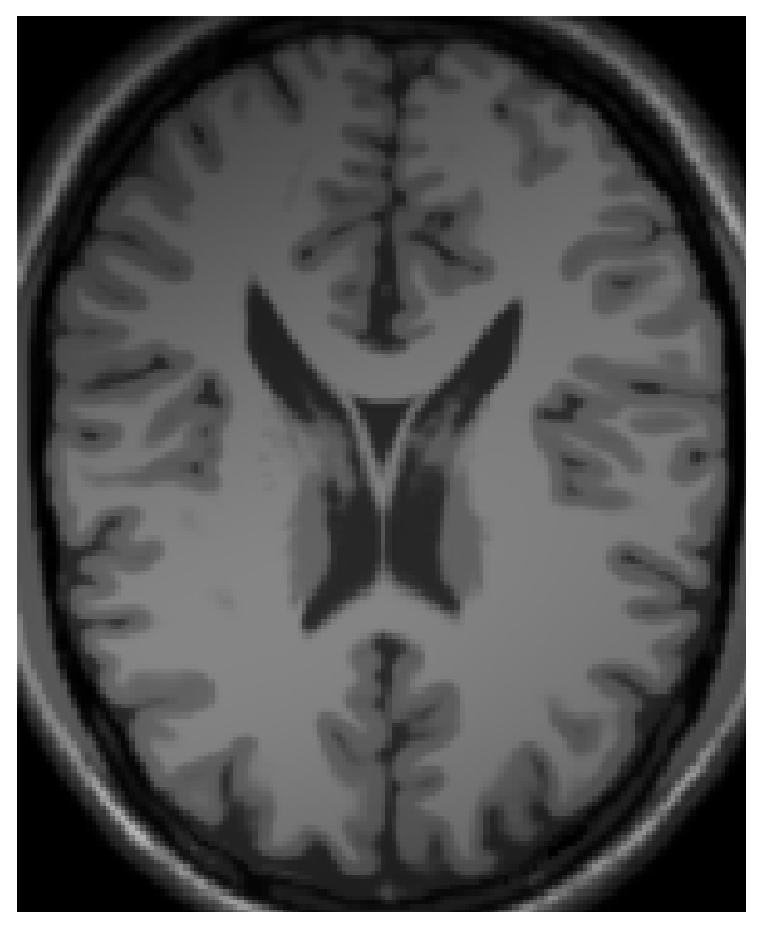
\includegraphics[height=41mm, angle=180]{eps/chapitre3/Brainweb_Bias_T1.eps}}
	\subfigure[]{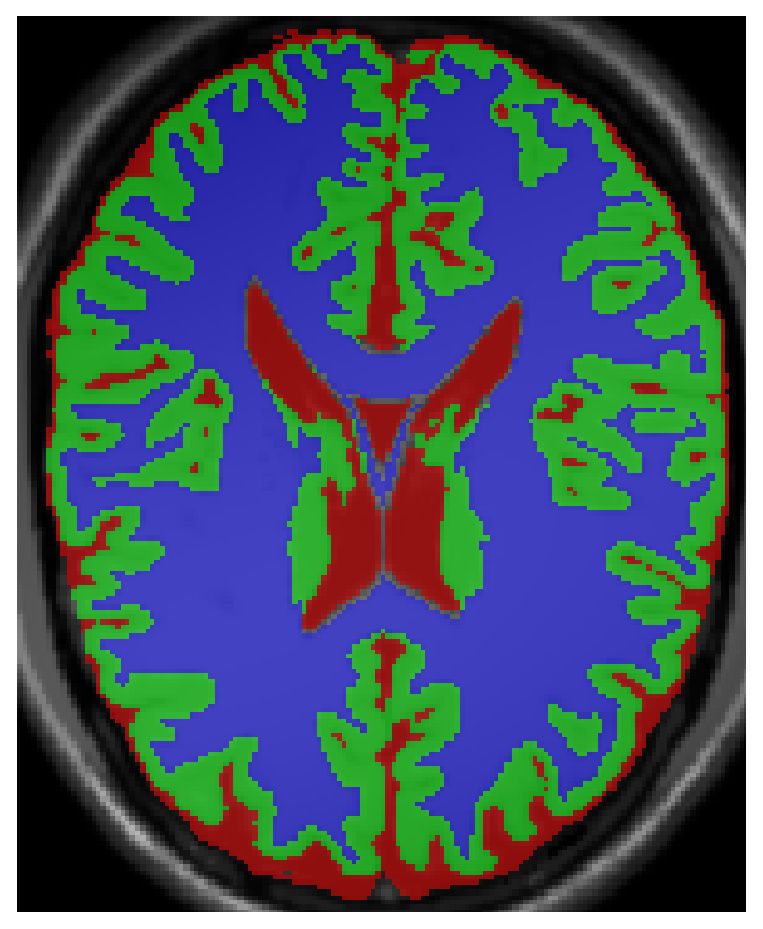
\includegraphics[height=41mm, angle=180]{eps/chapitre3/Brainweb_Bias_truth.eps}}
	\subfigure[]{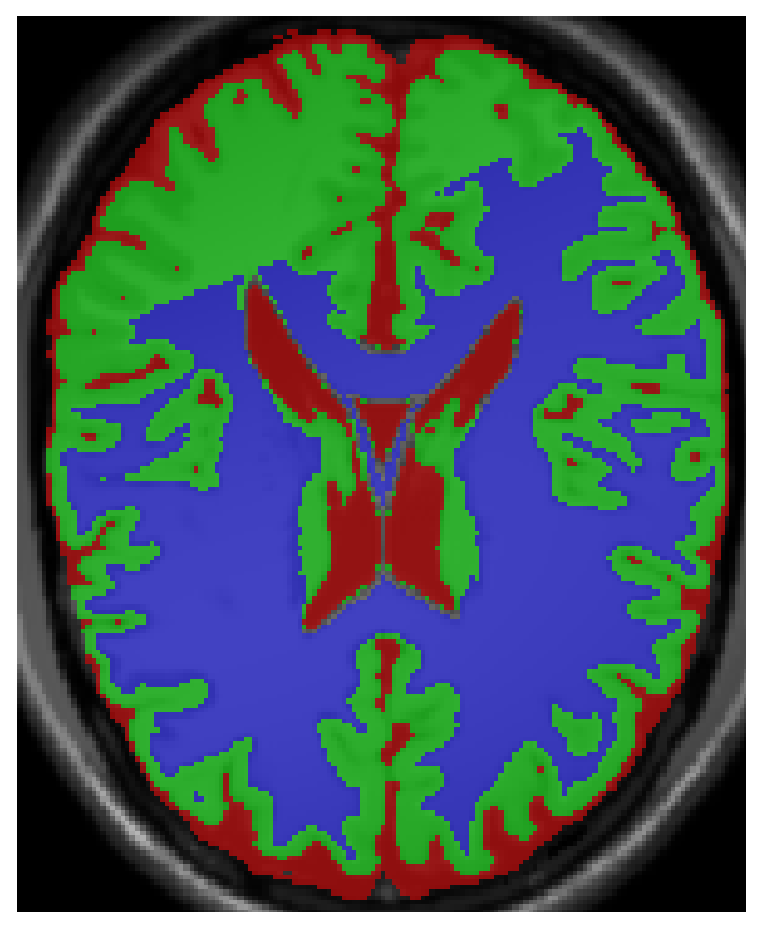
\includegraphics[height=41mm, angle=180]{eps/chapitre3/Brainweb_Bias_classicfcm.eps}}
	\subfigure[]{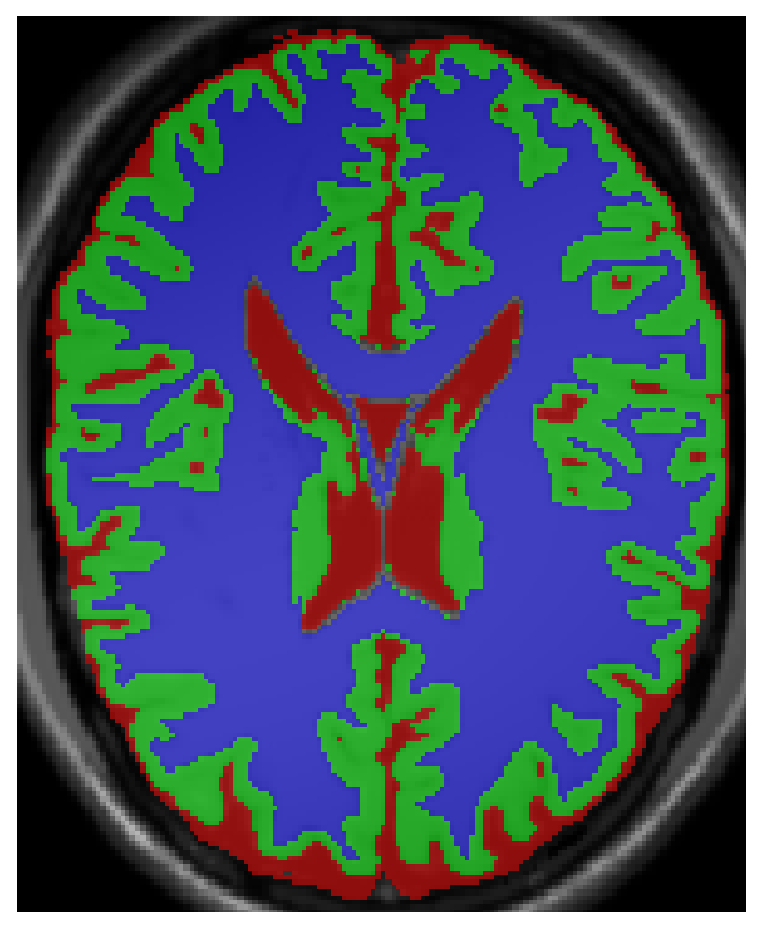
\includegraphics[height=41mm, angle=180]{eps/chapitre3/Brainweb_Bias_nlfcm.eps}}
        \end{center}

        \caption[R�sultats de la segmentation d'une image T1 pr�sentant un biais en intensit�]{\emph{R�sultats de la segmentation d'une image T1 pr�sentant un biais en intensit�. (a) Coupe d'une image T1. (b) V�rit� terrain. (c) Segmentation par FCM classique. (d) Segmentation par FCM non-local.}}

        \label{FIG:VIEW:BRAINWEB:BIAS}

\end{figure}

Nous pouvons observer que l'algorithme FCM non local obtient les meilleurs scores selon les taux de recouvrement.
Elle apporte une prise en compte du biais en intensit� � l'algorithme FCM sans en n�cessiter une �valuation explicite.


\subsubsection{\'Evaluation du terme de r�gularisation}
\label{sec:brainweb:nlReg}

L'algorithme NL-Reg est initialis� par un algorithme des K-Moyennes de mani�re � obtenir une premi�re estimation de la distribution en intensit� et les cartes de probabilit� sont initialis�es � $\frac{1}{C}$ ($C$ �tant le nombre de classes recherch�es).
Dans un premier temps, des tests sont r�alis�s sur une image bruit�e � $5$~\% afin d'�valuer l'influence des param�tres non-locaux sur la segmentation.
Enfin, diff�rentes segmentations sont r�alis�es avec les param�tres optimaux obtenus pour �tudier le comportement du terme de r�gularisation non-local en fonction du bruit.

\paragraph*{Influence des param�tres non-locaux}

\begin{figure}[!t]

        \begin{center}
	\subfigure[]{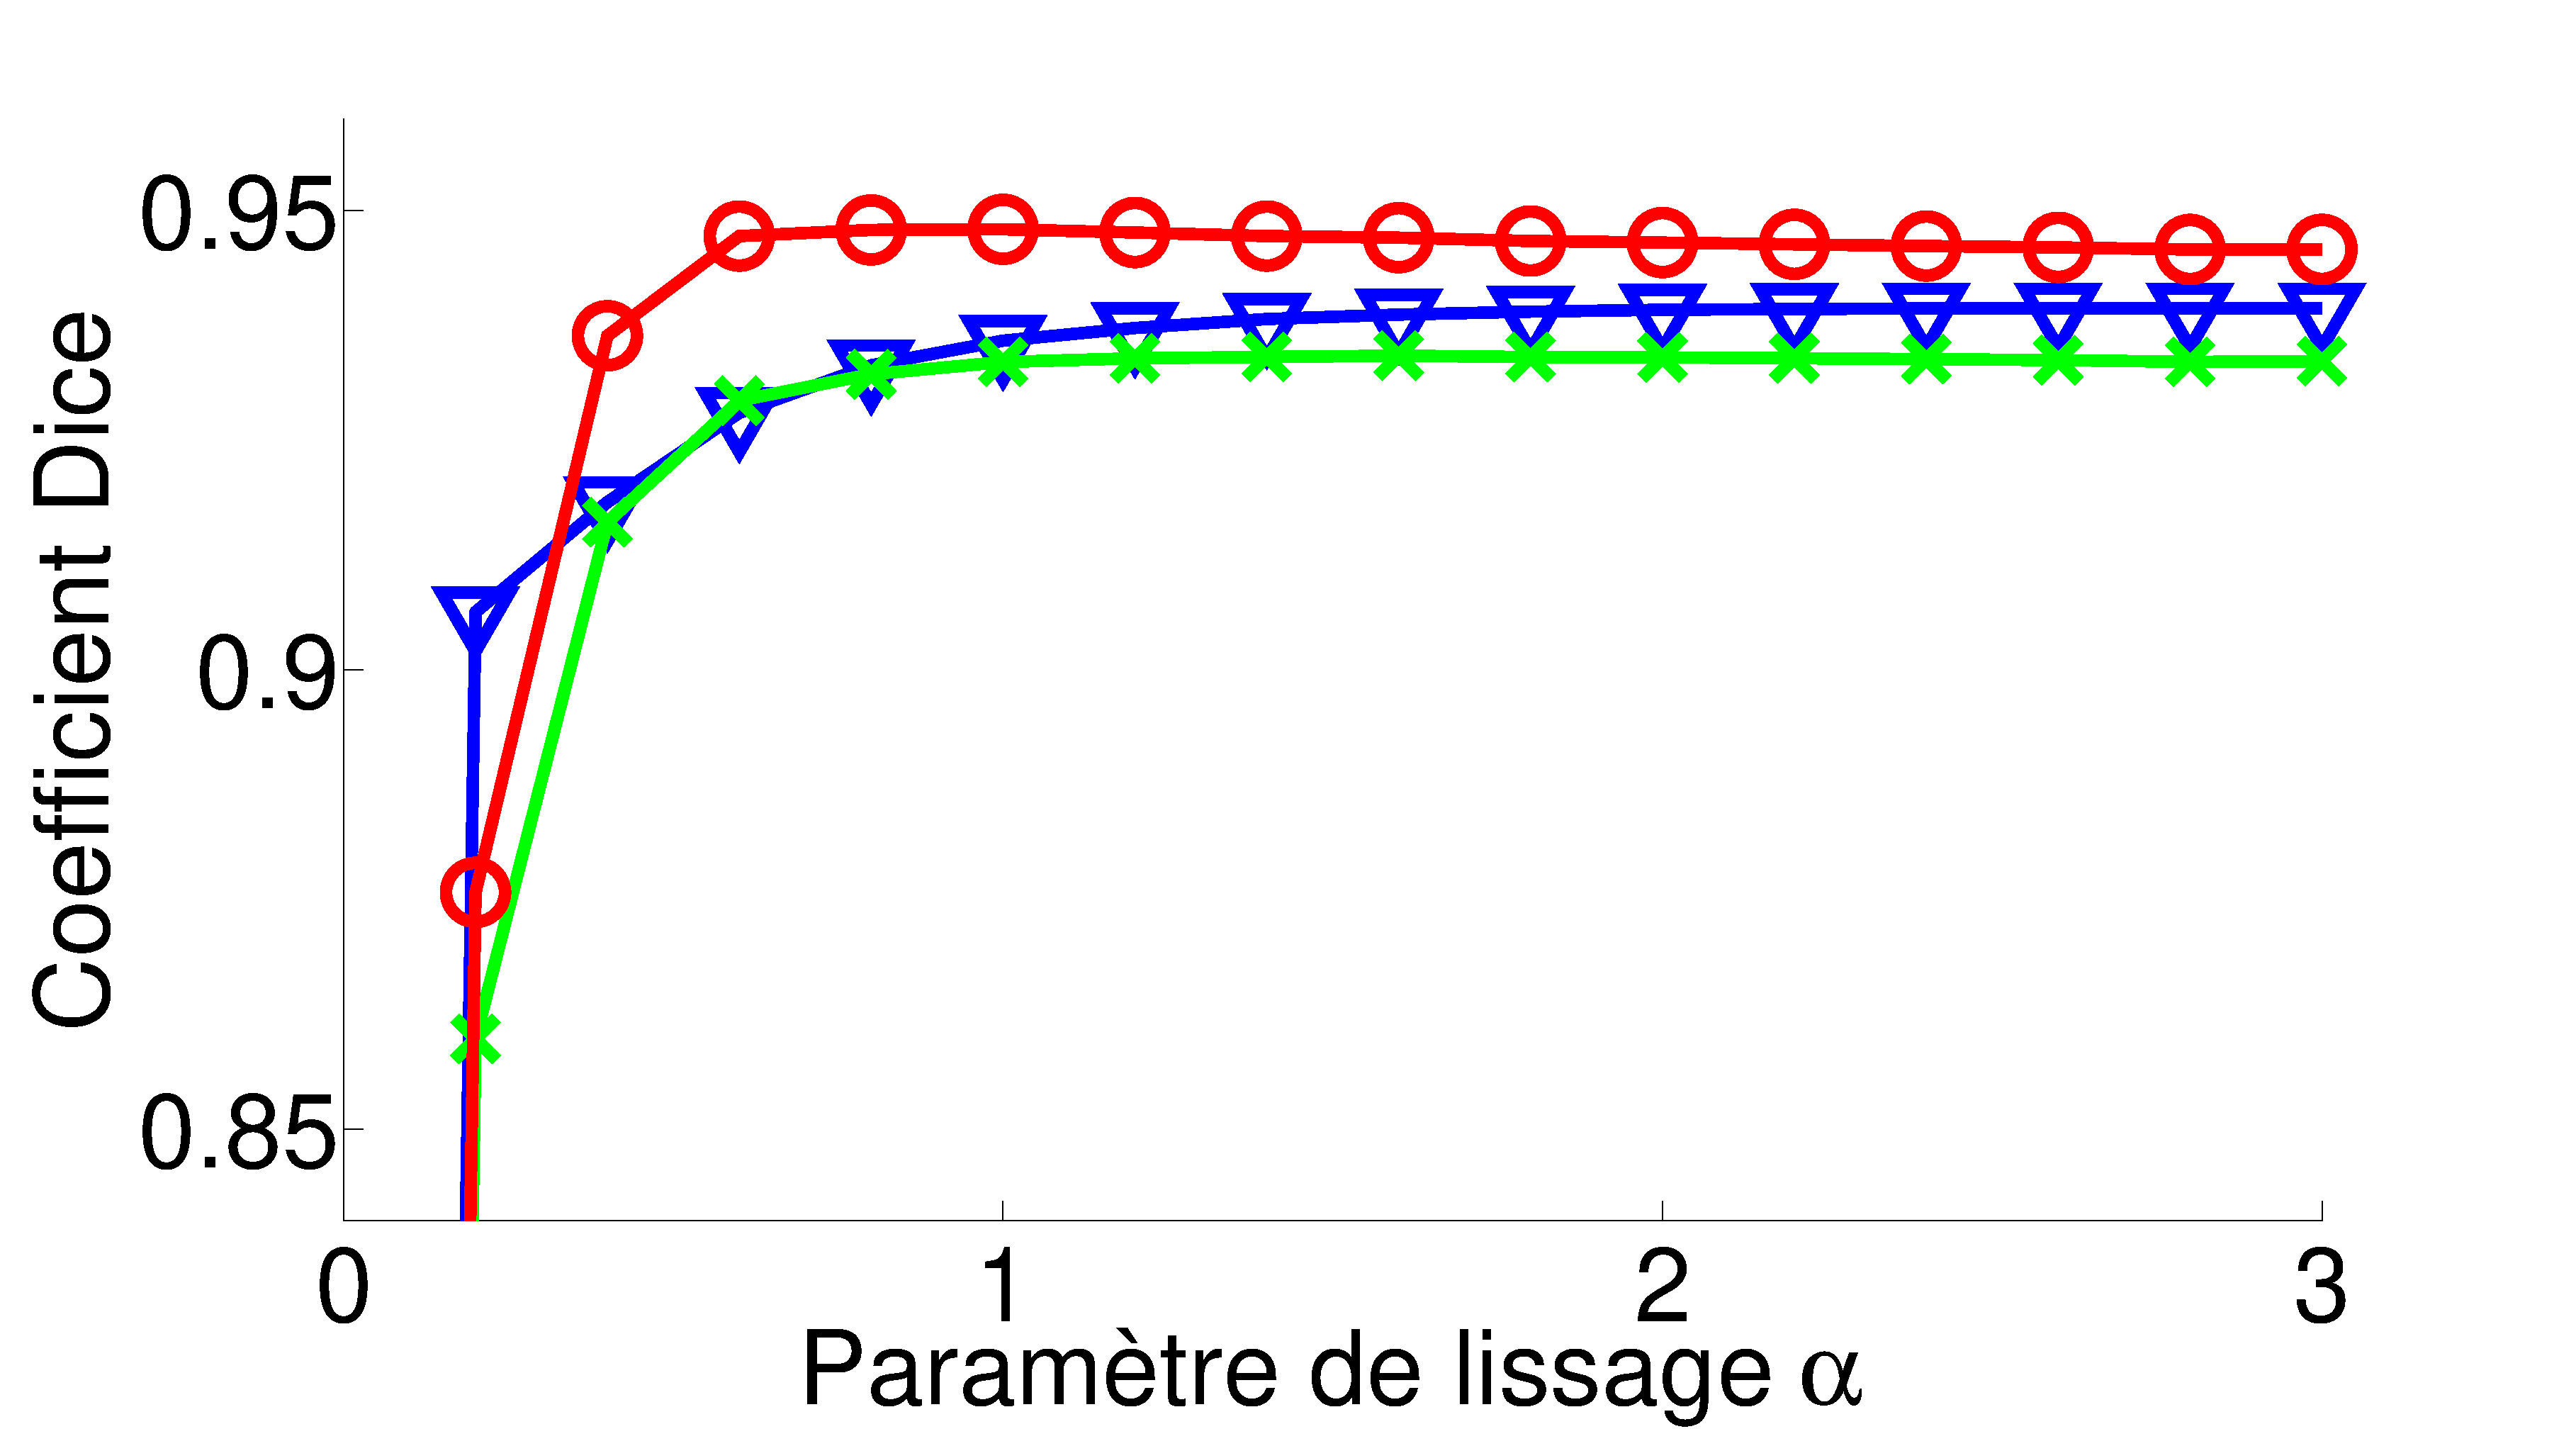
\includegraphics[height=38mm]{eps/chapitre3/nlreg_Dice_Smooth.eps}}
	\subfigure[]{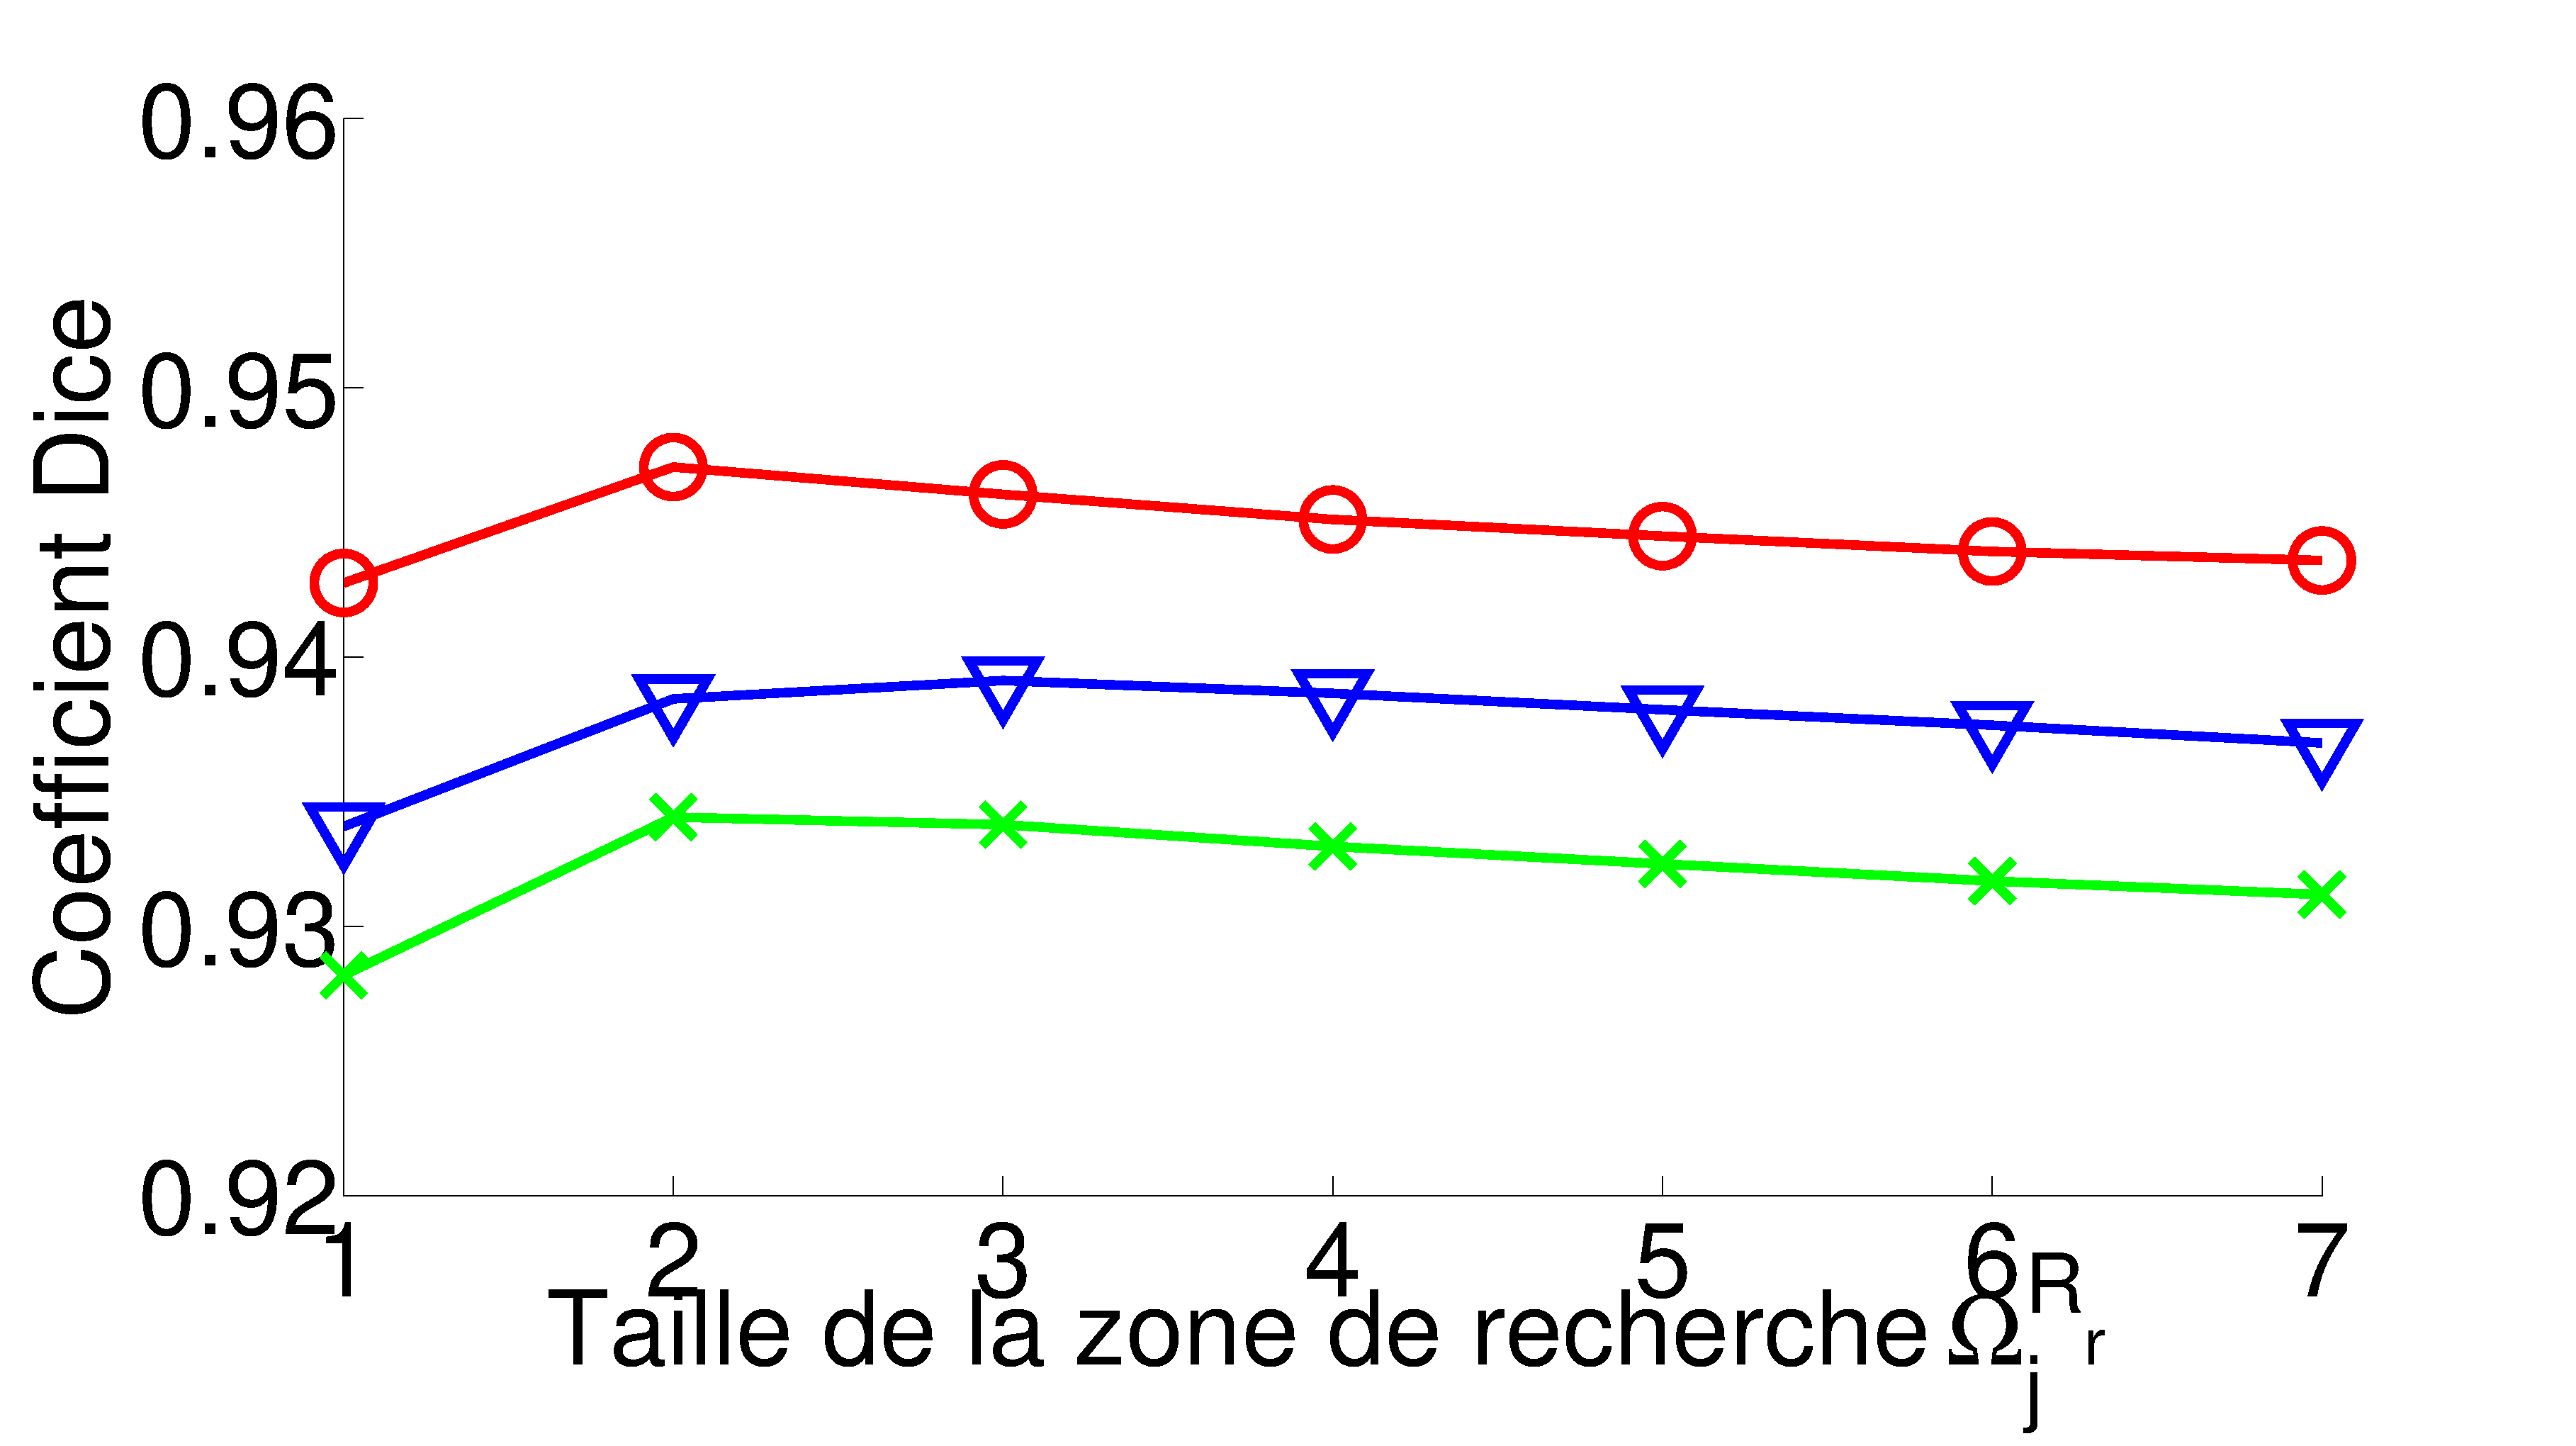
\includegraphics[height=38mm]{eps/chapitre3/nlreg_Dice_HWVS.eps}\label{FIG:PARAM:BRAINWEB:NOISE:HWVS}}
        \end{center}
        
        \caption[Etude de l'influence du param�tre de lissage $\alpha$ et du rayon de la zone de recherche $\Omega^{R_{r}}_{j}$]{\emph{(a) Coefficient Dice en fonction du param�tre de lissage $\alpha$. (b) Coefficient Dice en fonction du rayon de la zone de recherche $\Omega^{R_{r}}_{j}$. LCR : $\bigtriangledown$, mati�re grise : $\times$, mati�re blanche : $\circ$.}}
        
        \label{FIG:PARAM:BRAINWEB:NOISE}

\end{figure}

Les param�tres test�s sont la taille de la zone de recherche $\lvert \Omega^{R_{r}}_{j} \rvert$ ainsi que le param�tre de lissage $\alpha$.
La figure \ref{FIG:PARAM:BRAINWEB:NOISE} fournit une indication de l'influence de ces deux param�tres sur la segmentation.
Le param�tre de lissage $\alpha$ a une forte influence sur la segmentation s'il est situ� entre $0$ et $1.5$, puis un ph�nom�ne de convergence est observ�. 
Dans la suite du manuscrit, il sera fix� � $1.5$.
Concernant la taille de la zone de recherche, la figure~\ref{FIG:PARAM:BRAINWEB:NOISE:HWVS} montre un maximum du taux de recouvrement avec un rayon de $2$ voxels pour la mati�re blanche et la mati�re grise, et un maximum avec un rayon de $3$ voxels pour le LCR.
Le rayon de la zone de recherche $\Omega^{R_r}_{j}$ est donc fix�e � $2$ pour la suite du manuscrit. 

\paragraph*{Comparaison par rapport � d'autres m�thodologies}

La comparaison inclut une �valuation des m�thodes FCM classique et RFCM \cite{Pham:CVIU:2001} en plus des m�thodes markoviennes.
Elle est effectu�e en simulant des segmentations avec un bruit ricien allant de $0$ � $9$~\%. 

La figure~\ref{FIG:VIEW:BRAINWEB:NOISE} pr�sente une coupe axiale d'une image T1 et les segmentations correspondantes pour les algorithmes FCM classique, RFCM \cite{Pham:CVIU:2001} et NL-Reg.
L'apport de RFCM par rapport � l'algorithme FCM classique est visible par l'absence d'art�facts de segmentation dus au bruit (par exemple : voxels class�s comme mati�re grise au milieu de la mati�re blanche).
Cependant, l'effet de lissage apport� par cette r�gularisation a pour effet de gommer les asp�rit�s dans certaines parties de l'image. 
Par exemple, une comparaison visuelle avec la v�rit� terrain montre une sous-segmentation du LCR au sein des sillons.
Le terme de r�gularisation non-local permet de rem�dier � cela gr�ce � la pond�ration introduite par les poids non-locaux, ce qui est illustr� par les figures~\ref{NLREG:ZOOM:TRUTH}, \ref{NLREG:ZOOM:RFCM} et \ref{NLREG:ZOOM:NLREG} montrant un zoom sur une zone particuli�re du cerveau.

De plus, le  tableau~\ref{TAB:DICE:BRAINWEB:NOISE} montre une meilleure performance des algorithmes FCM que des algorithmes bas�s sur les champs et cha�nes de Markov. 
La figure~\ref{FIG:DICE:BRAINWEB:NOISE}, comparant les coefficients Dice obtenus par les algorithmes en fonction du niveau de bruit, confirme cette observation.
Elle montre que le terme de r�gularisation non-local fournit une segmentation plus consistante � partir d'un niveau de bruit de $5$~\%.

\begin{table}[!t]
\begin{center}
\begin{tabular}{|l | *{3}{c|}}
	\hline
	M�thodes & LCR & Mati�re grise & Mati�re blanche \\
	\hline
	FCM & 90.46 & 84.36 & 85.48\\
	RFCM & 92.09 & 91.12 & 92.91\\
% 	R-FCM with adaptive weights & 92.76 & 91.09 & 92.49\\
% 	NL-Reg without adaptive weights & 92.22 & 92.22 & 94.12\\
	NL-Reg & \fbox{93.63} & \fbox{93.35} & \fbox{94.77}\\
	SPM5 \cite{Ashburner:NeuroImage:2005}& 54.2 & 85.1 & 87 \\
	EMS \cite{VanLeemput2:TMI:1999}& 89.6 & 86.9 & 90.9\\
	HMC \cite{Bricq:MIA:2008} & 68 & 86.5 & 87.1\\
	\hline 
\end{tabular}
% \vspace{2mm}
\caption[Coefficients Dice issus de diff�rentes segmentations d'une image pond�r�e en T1 avec un bruit ricien de $9$~\%]{\emph{Application de diff�rentes segmentations � une image pond�r�e en T1 avec un bruit ricien de $9$~\%. Comparaison des diff�rents coefficient Dice pour le LCR, la mati�re grise et la mati�re blanche.\label{TAB:DICE:BRAINWEB:NOISE}}}
\end{center}
\end{table}

\begin{figure}[!t]
\begin{center}
\subfigure[]{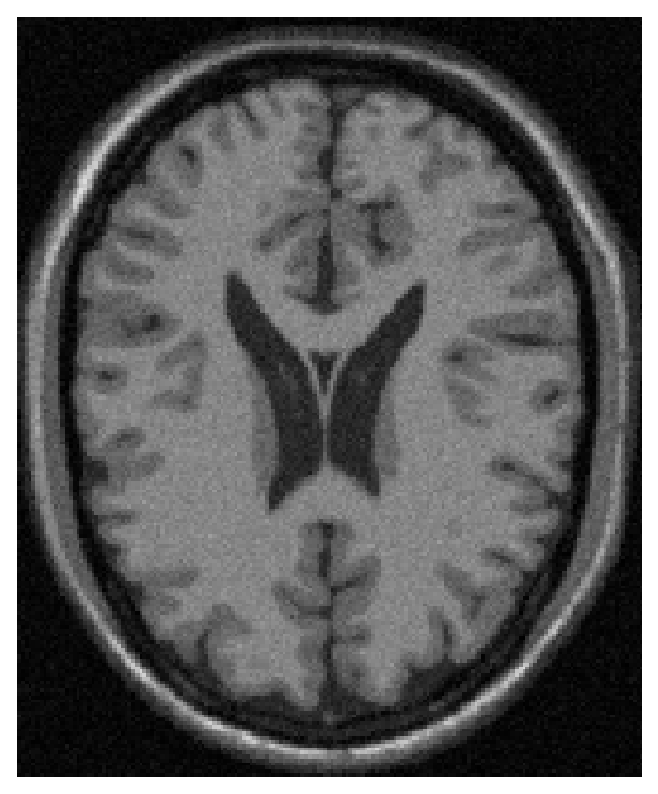
\includegraphics[height=45mm, angle=180]{eps/chapitre3/Brainweb_Noise_T1.eps}}  
\subfigure[]{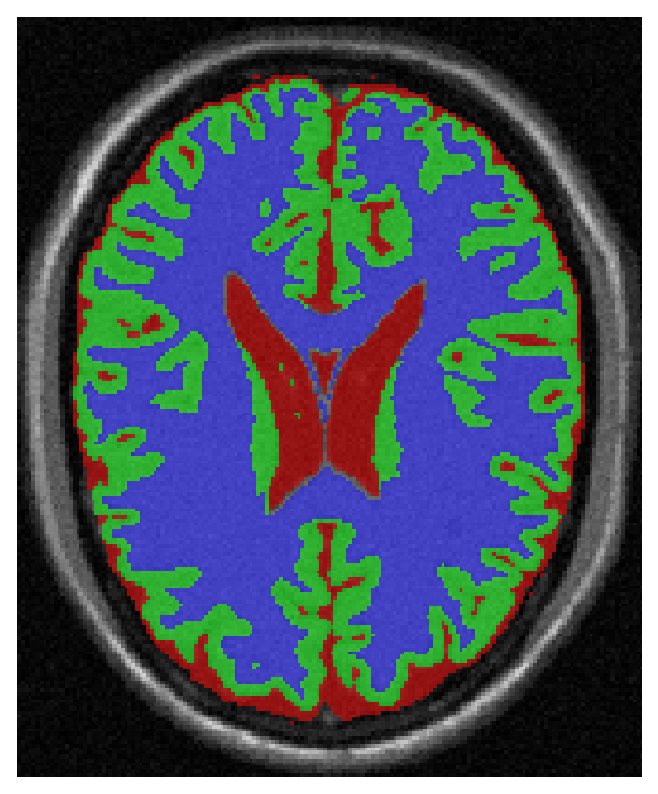
\includegraphics[height=45mm, angle=180]{eps/chapitre3/Brainweb_Noise_truth.eps}}\\
\subfigure[]{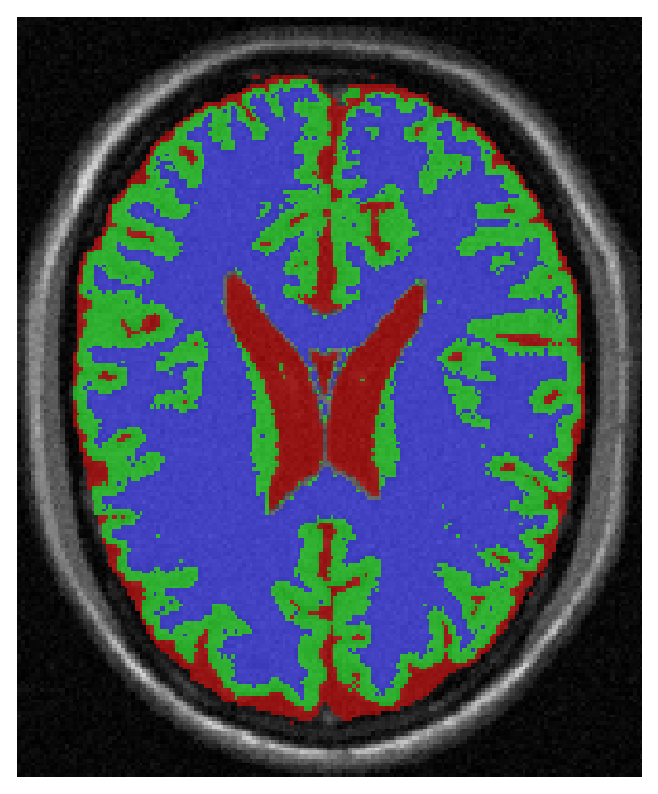
\includegraphics[height=45mm, angle=180]{eps/chapitre3/Brainweb_Noise_classicfcm.eps}}  
\subfigure[]{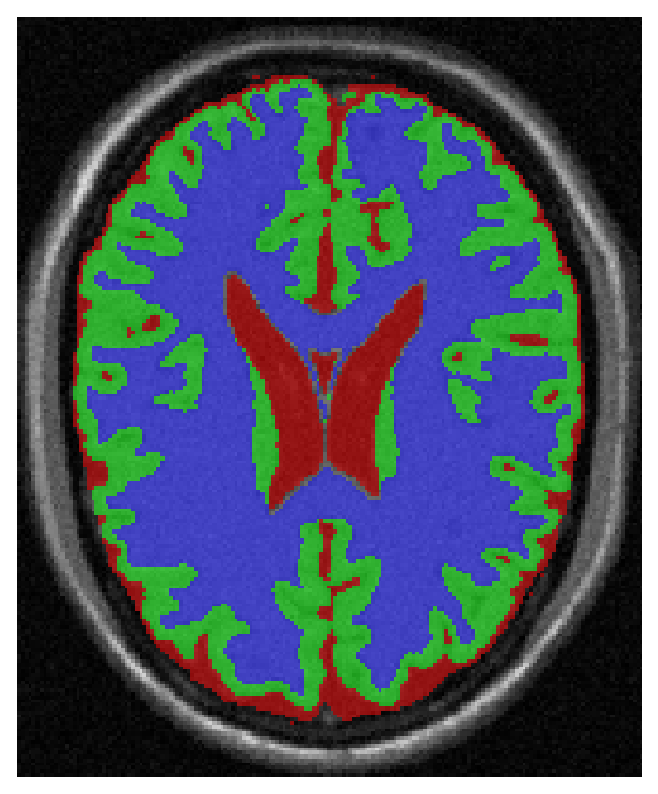
\includegraphics[height=45mm, angle=180]{eps/chapitre3/Brainweb_Noise_rfcm.eps}}  
\subfigure[]{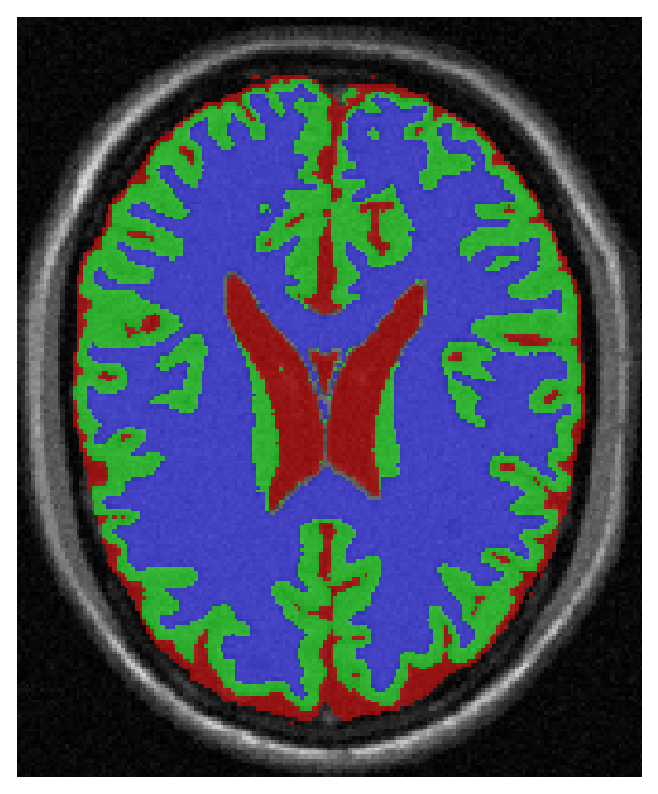
\includegraphics[height=45mm, angle=180]{eps/chapitre3/Brainweb_Noise_nlregfcm.eps}}\\
\subfigure[]{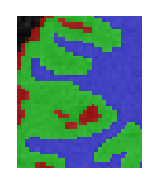
\includegraphics[height=45mm, angle=180]{eps/chapitre3/Brainweb_Noise_truth_zoom.eps}\label{NLREG:ZOOM:TRUTH}}  
\subfigure[]{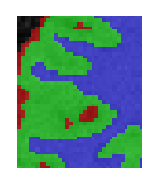
\includegraphics[height=45mm, angle=180]{eps/chapitre3/Brainweb_Noise_rfcm_zoom.eps}\label{NLREG:ZOOM:RFCM}}  
\subfigure[]{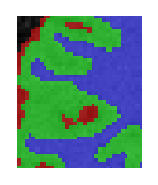
\includegraphics[height=45mm, angle=180]{eps/chapitre3/Brainweb_Noise_nlregfcm_zoom.eps}\label{NLREG:ZOOM:NLREG}}\\
\caption[Aper�u de diff�rentes segmentations d'une image pond�r�e en T1 avec un bruit ricien de $5$~\%]{\emph{(a) Coupe axiale d'une image pond�r�e en T1 avec un bruit ricien de $5$~\%. (b) V�rit� terrain. (c) Segmentation par FCM classique. (d) Segmentation par RFCM~\cite{Pham:CVIU:2001}. (e) Segmentation par NL-Reg. (f) Zoom sur la v�rit� terrain. (g) Zoom sur la segmentation par RFCM. (h) Zoom sur la segmentation par NL-Reg.}\label{FIG:VIEW:BRAINWEB:NOISE}}
\end{center}
\end{figure}

\begin{figure}[!t]
\begin{center}
\subfigure[]{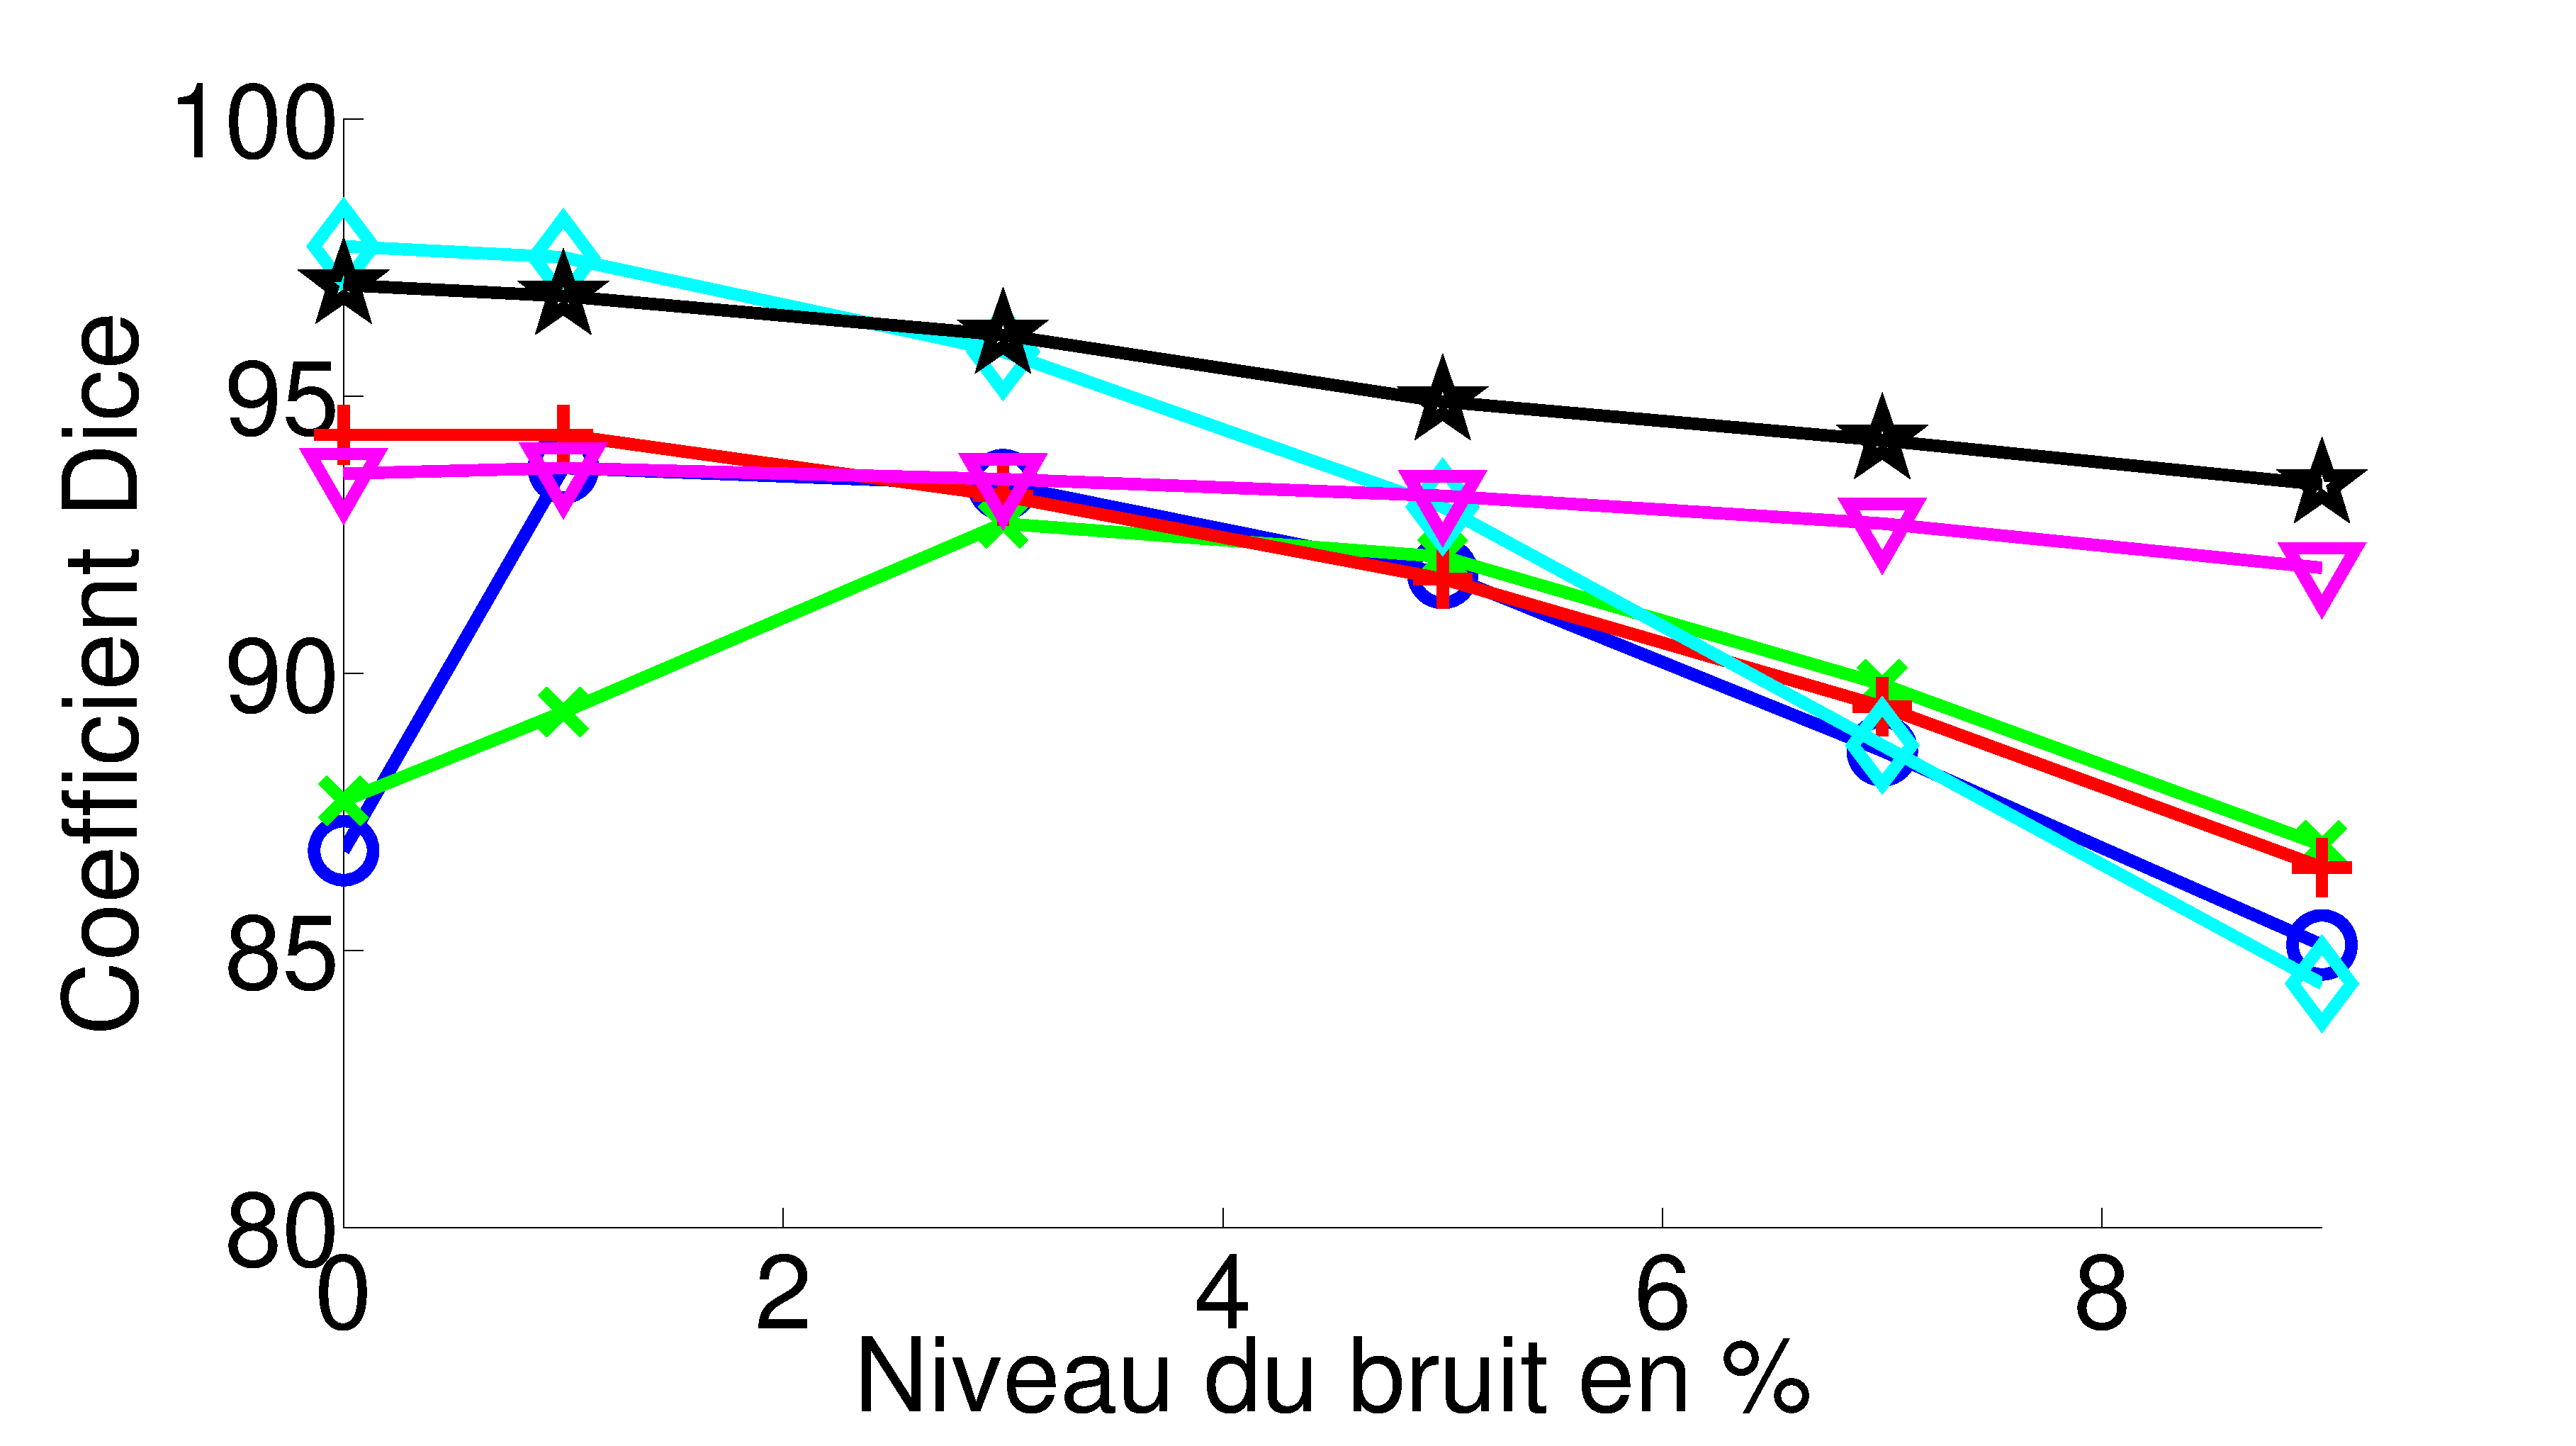
\includegraphics[height=38mm]{eps/chapitre3/GM_Noise_Dice_Brainweb.eps}}  
\subfigure[]{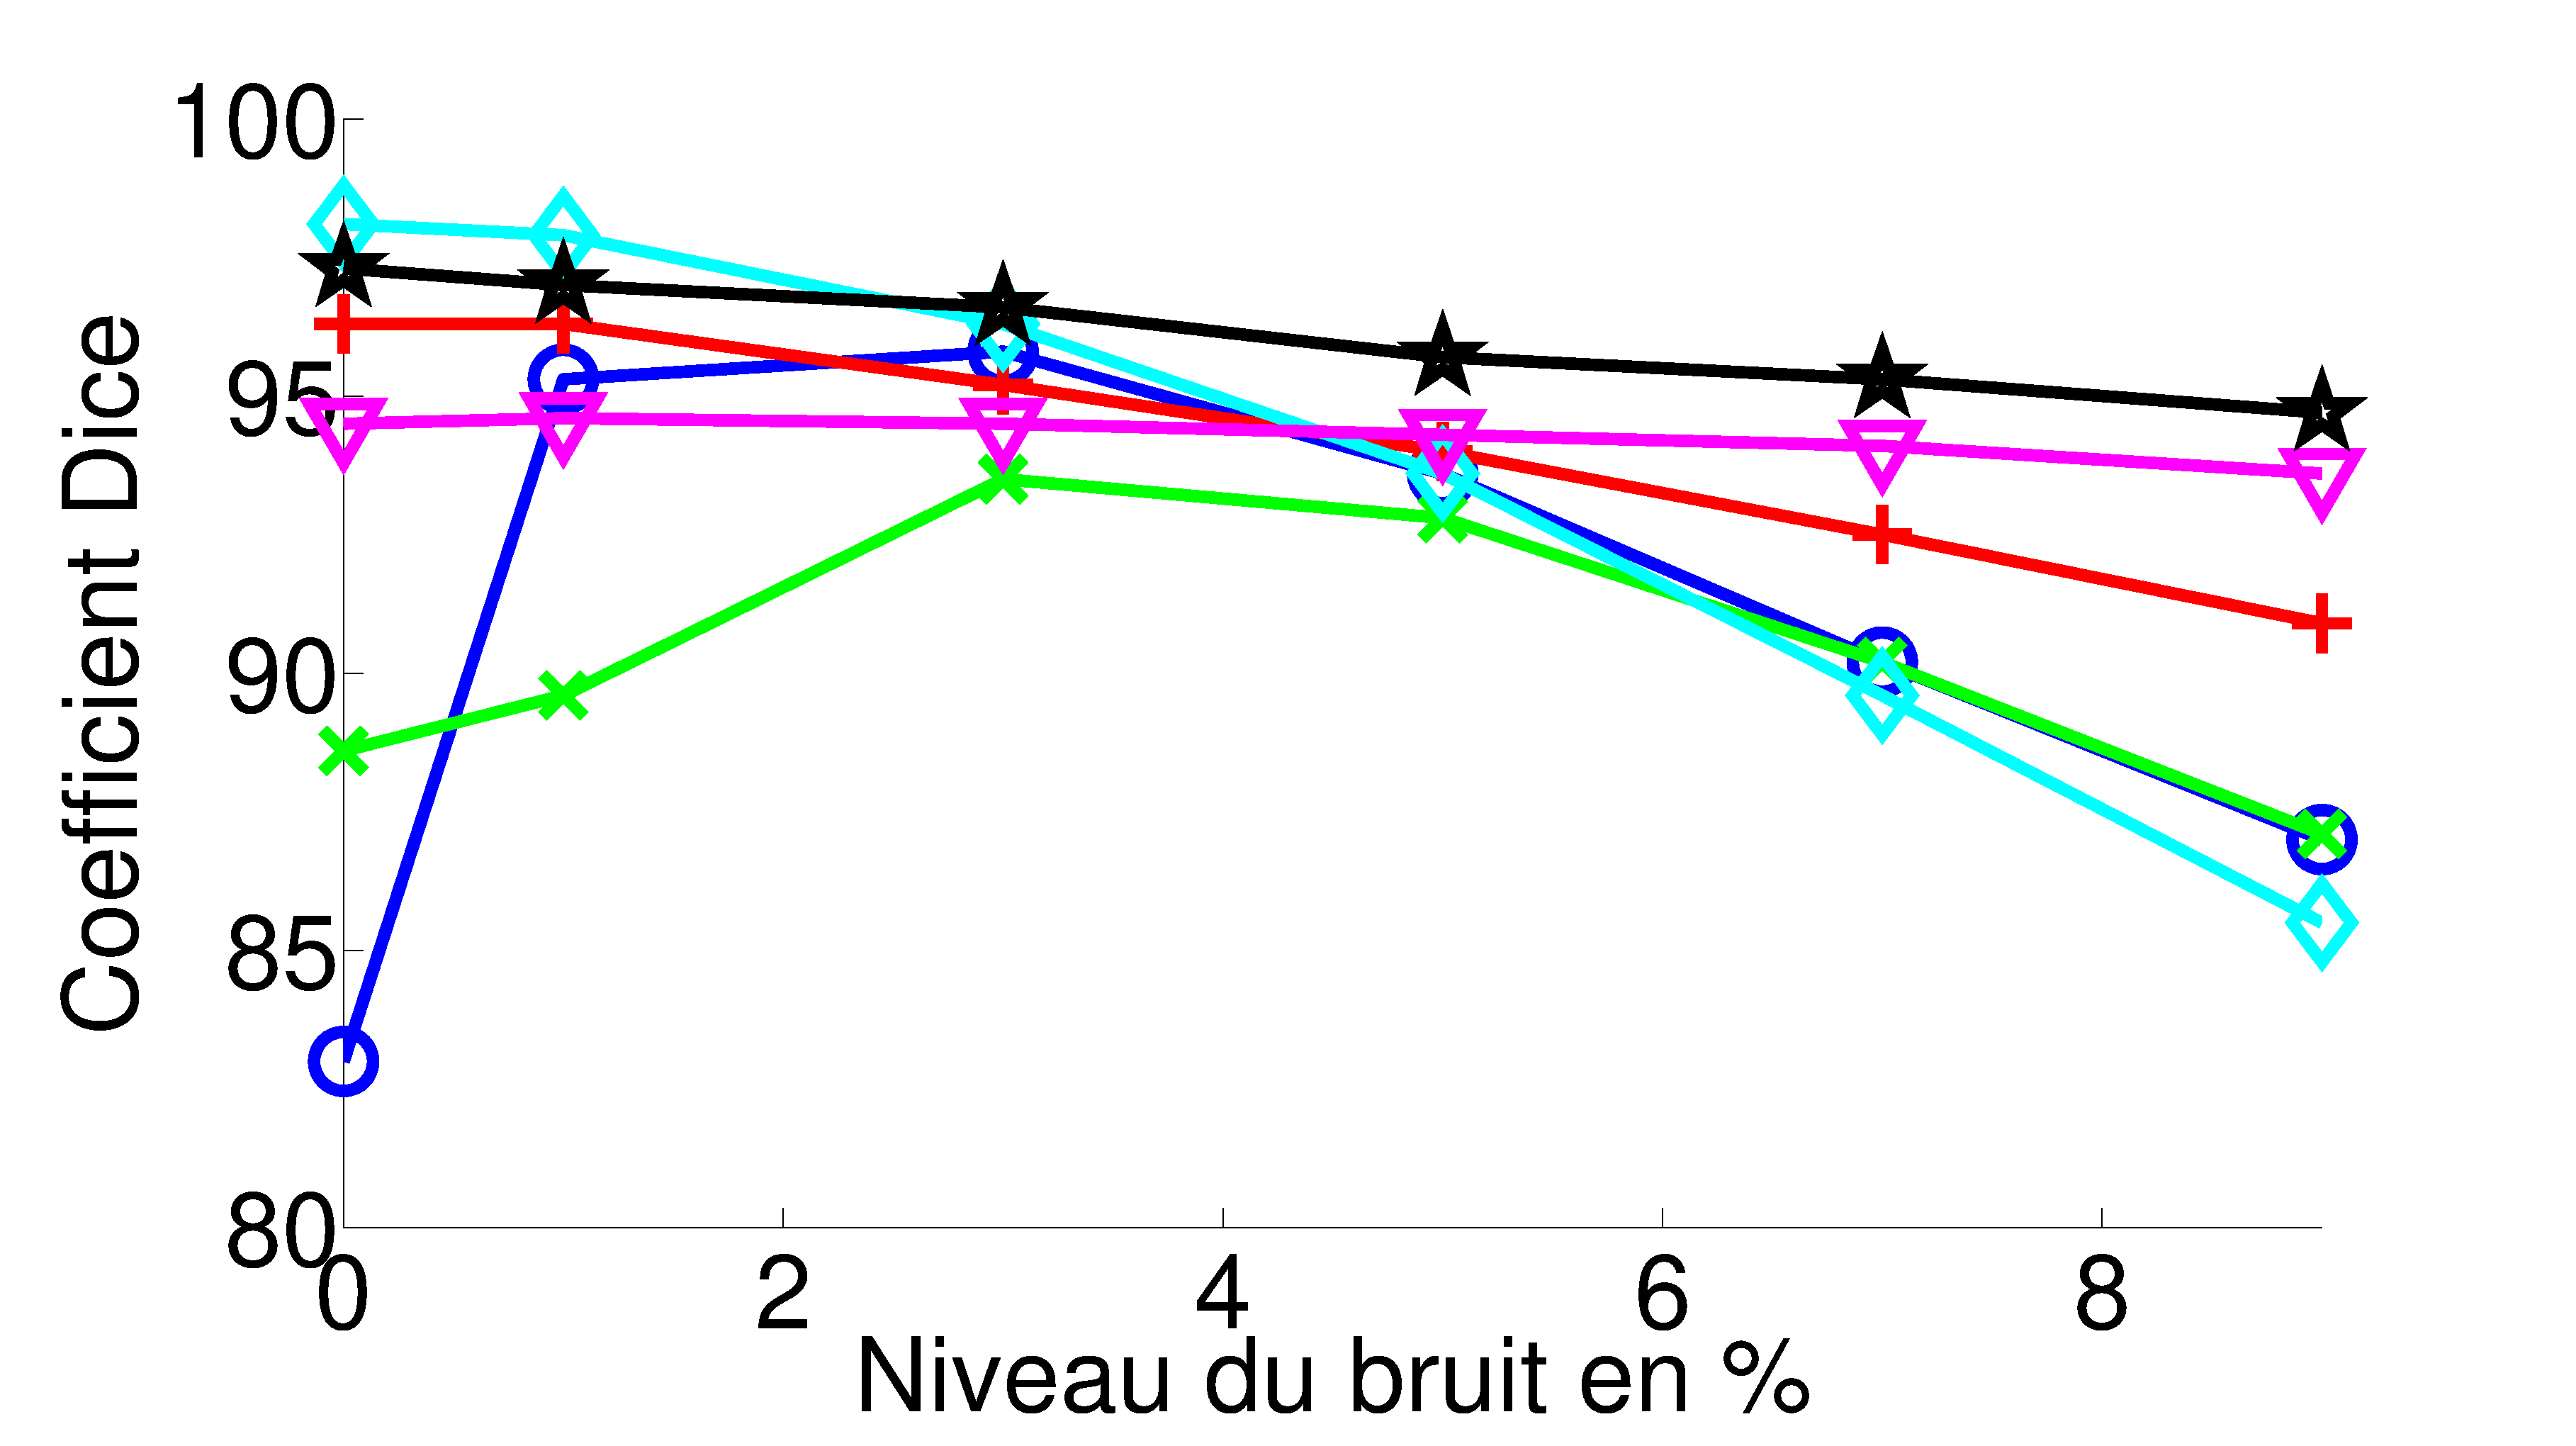
\includegraphics[height=38mm]{eps/chapitre3/WM_Noise_Dice_Brainweb.eps}}  
\caption[\'Evolution du coefficient Dice en fonction du bruit pour diff�rentes m�thodologies]{\emph{\'Evolution du coefficient Dice en fonction du bruit pour diff�rentes m�thodologies. (a) Mati�re grise. (b) Mati�re blanche. L�gende : SPM5 : $\circ$, EMS : $\times$, HMC : $+$, FCM : $\diamond$, RFCM : $\bigtriangledown$, NL-Reg : $\star$.}\label{FIG:DICE:BRAINWEB:NOISE}}
\end{center}
\end{figure}

\subsubsection{Association des termes d'attache aux donn�es et de r�gularisation non-locaux}
\label{sec:brainweb:nlAll}

% L'association des termes non-locaux devrait permettre de segmenter des images corrompues par un biais en intensit� et par un bruit ricien. 
% Au cours de ces exp�riences, le biais en intensit� est de l'ordre de 20\% et le bruit est de type Ricien allant de 1\% � 9\%.
Dans cette section, l'association des termes d'attache aux donn�es et de r�gularisation non-locaux est �valu�e.
Les images utilis�es pr�sentent un biais en intensit� de $20$~\% et un bruit de type ricien d'un niveau allant de $0$~\% � $9$~\%.
Les param�tres consid�r�s sont les suivants : 
\begin{itemize}
\item la taille des sous-volumes destin�s � �valuer le mod�le de la distribution d'intensit� est fix�e � $M_j = 17\times17\times17$, 
\item la taille de la zone de recherche destin�e au calcul des poids non-locaux du terme d'attache aux donn�es est fix�e � $\Omega^{R_{d}}_{j} = 17\times17\times17$, 
\item la taille de la zone de recherche destin�e au calcul des poids non-locaux du terme de r�gularisation est fix�e � $\Omega^{R_{r}}_{j} = 5\times5\times5$,
\item le param�tre de lissage pour le calcul des poids non-locaux est fix� � $\alpha = 1.5$.
\end{itemize}

Les r�sultats sont fournis par la figure~\ref{FIG:VIEW:BRAINWEB:ALL} et la table~\ref{TAB:DICE:BRAINWEB:ALL}.
L'utilisation du terme d'attache aux donn�es non-local permet d'am�liorer largement les performances par comparaison avec l'algorithme FCM original.
De plus, l'ajout du terme de r�gularisation non-local permet de combiner les avantages des deux termes et de fournir une segmentation consistante malgr� la pr�sence d'un biais en intensit� et de bruit.
% De plus, l'utilisation simultan�e des termes non-locaux am�ne une am�lioration conjointe des r�sultats et permet d'obtenir de meilleurs r�sultats finaux.

\begin{figure}[!t]

        \begin{center}
	\subfigure[]{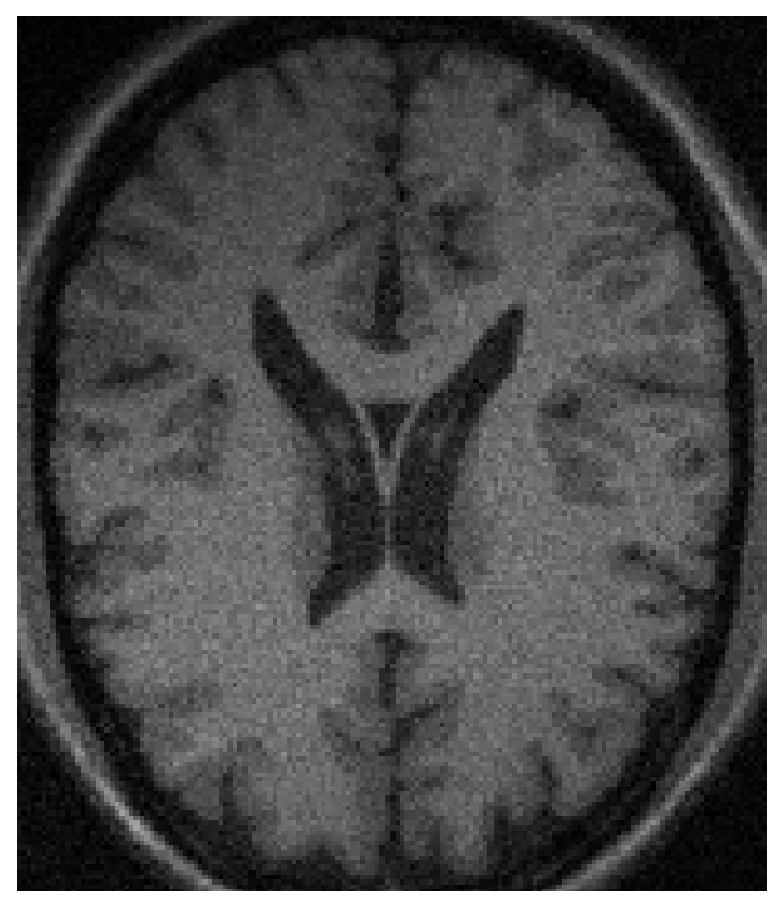
\includegraphics[height=41mm, angle=180]{eps/chapitre3/Brainweb_All_T1.eps}}
	\subfigure[]{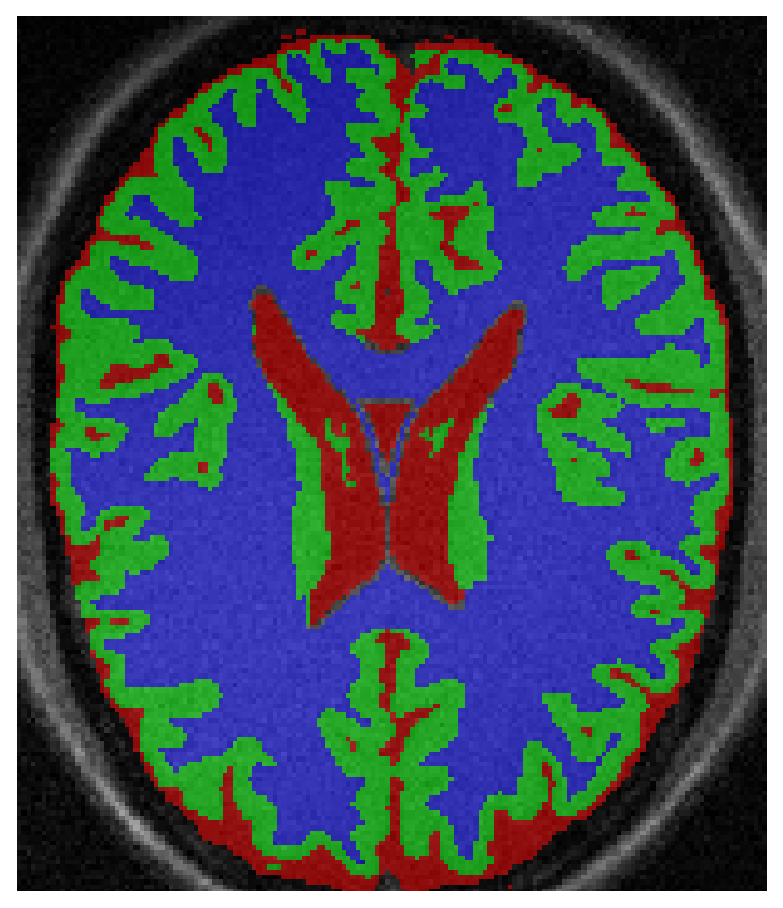
\includegraphics[height=41mm, angle=180]{eps/chapitre3/Brainweb_All_Truth.eps}}\\
	\subfigure[]{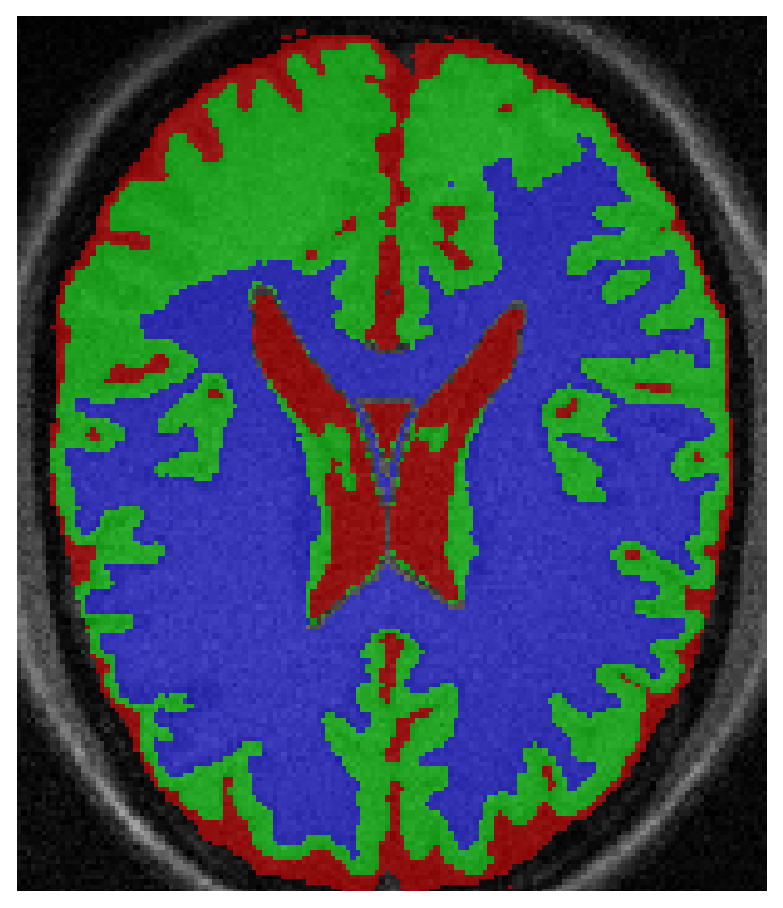
\includegraphics[height=41mm, angle=180]{eps/chapitre3/Brainweb_All_NLReg.eps}}
	\subfigure[]{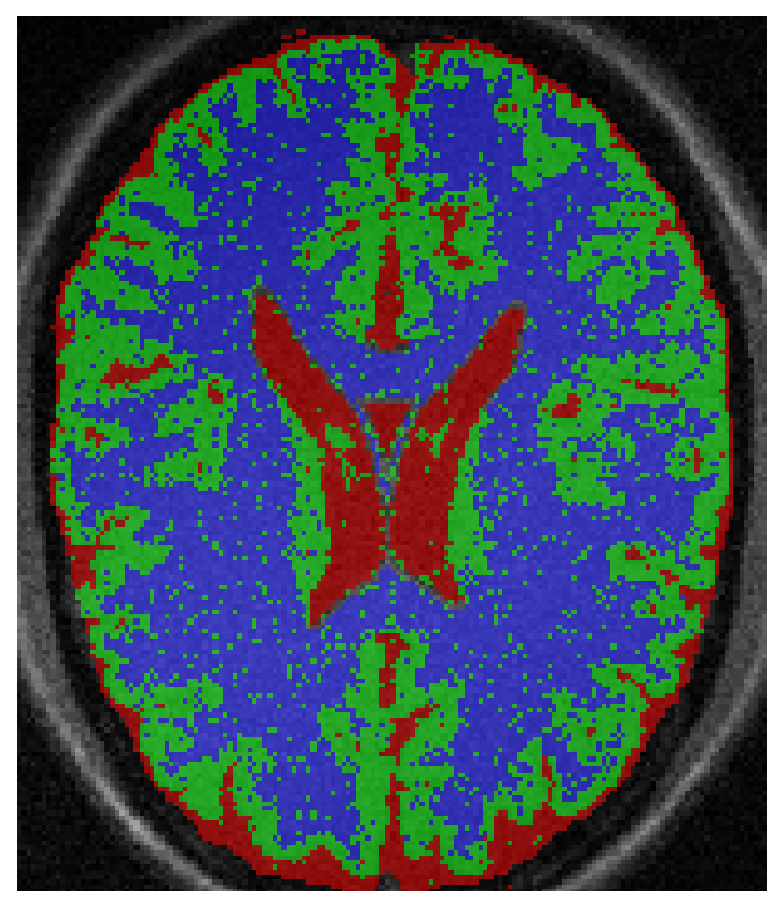
\includegraphics[height=41mm, angle=180]{eps/chapitre3/Brainweb_All_NLFCM.eps}}
	\subfigure[]{\includegraphics[height=41mm, angle=180]{eps/chapitre3/Brainweb_All_NLRFCM.eps}}
        \end{center}

        \caption[R�sultats de la segmentation d'une image T1 pr�sentant une inhomog�n�it� en intensit� et un bruit ricien de $9$~\%]{\emph{R�sultats de la segmentation d'une image T1 pr�sentant une inhomog�n�it� en intensit� et un bruit ricien de $9$~\%. (a) Coupe d'une image T1. (b) V�rit� terrain. (c) Segmentation par NL-Reg. (d) Segmentation par NL-FCM. (e) Segmentation par NL-R-FCM.}}

        \label{FIG:VIEW:BRAINWEB:ALL}

\end{figure}

\begin{table}[!t]
\begin{center}
\begin{tabular}{|l | *{2}{c|}}
	\hline
	M�thodes & Mati�re grise & Mati�re blanche \\
	\hline
	SPM5 \cite{Ashburner:NeuroImage:2005} & 85.1 & 87 \\ 
	EMS \cite{VanLeemput2:TMI:1999} & 86.9 & 87.1 \\
	HMC \cite{Bricq:MIA:2008} & \fbox{86.5} & \fbox{90.9}  \\
	\hline
	FCM \cite{Pham:TMI:1999} &  62.09 & 69.98\\
	NL-Reg  & 64.25 & 72.16\\
	NL-FCM & 82.0 & 84.7\\
	NL-R-FCM & \fbox{86.5} & 89.2\\
	\hline 
\end{tabular}
\vspace{2mm}
\caption[Coefficients Dice issus diff�rentes segmentation sur une image T1 issue de BrainWeb avec un bruit Ricien � $9$~\% et un biais en intensit� de $20$~\%]{Application de diff�rentes segmentation sur une image T1 issue de BrainWeb avec un bruit Ricien � $9$~\% et un biais en intensit� de $20$~\%. Comparaison des diff�rents coefficient Dice pour la mati�re grise et la mati�re blanche (Coefficients Dice pour SPM5, EMS et HMC issus de \cite{Bricq:MIA:2008}).\label{TAB:DICE:BRAINWEB:ALL}}
\end{center}
\end{table}

\begin{figure}[!t]

        \begin{center}
	\subfigure[]{\includegraphics[height=38mm]{eps/chapitre3/Brainweb_All_GM.eps}}
	\subfigure[]{\includegraphics[height=38mm]{eps/chapitre3/Brainweb_All_WM.eps}}\\
        \end{center}

        \caption[\'Evolution du coefficient Dice en fonction du bruit pour diff�rentes m�thodologies]{\emph{\'Evolution du coefficient Dice en fonction du bruit pour diff�rentes m�thodologies. (a) Mati�re grise. (b) Mati�re blanche. L�gende : SPM5 : $\circ$, EMS : $\times$, HMC : $+$, NL-Reg : $\diamond$, NL-FCM : $\bigtriangledown$, NL-R-FCM : $\star$ (Coefficients Dice pour SPM5, EMS et HMC issus de \cite{Bricq:MIA:2008}).}}

        \label{FIG:DICE:BRAINWEB:ALL}

\end{figure}

La figure~\ref{FIG:DICE:BRAINWEB:ALL} montre l'�volution des performances des diff�rentes m�thodologies avec un bruit ricien allant de $0$ � $9$~\% dans le cas de la mati�re blanche et de la mati�re grise. 
Ces deux graphiques illustrent la similarit� des performances de la m�thode non-locale par rapport aux algorithmes bas�es sur les champs et cha�nes de Markov.
Une diff�rence significative n'est observable qu'� partir d'un niveau de bruit �lev� ($7$~\%) et seulement dans le cas de la mati�re blanche. 
De plus, dans ce cas pr�cis, la m�thode HMC semble l�g�rement sup�rieure.

\subsection{IBSR}
\label{sec:ibsr}

Cette base, �galement disponible sur internet~\footnote{\url{http://www.cma.mgh.harvard.edu/ibsr/}}, est fournie par le Center for Morphometric Analysis du Massachussetts General Hospital.
Elle est compos�e de 18 volumes pond�r�s en T1 acquis sur des patients sains.
La taille de ces volumes est $128\times256\times256$ et chaque image dispose d'une v�rit�-terrain, comprenant le LCR, la mati�re blanche et la mati�re grise, r�alis�e par des experts.

\begin{table}[!t]
\begin{center}
\begin{tabular}{|l|c p{1.5cm}|c p{1.5cm}|}
	\hline
	M�thodes & \multicolumn{2}{|c|}{Mati�re Blanche (\%)} & \multicolumn{2}{|c|}{Mati�re Grise (\%)} \\
	& Moyenne & \centering{\'Ecart-Type} & Moyenne & \centering{\'Ecart-Type} \tabularnewline
	\hline
	SPM 5 \cite{Ashburner:NeuroImage:2005} & 85.27 & \centering 5.52 & 78.7 & \centering 13.98 \tabularnewline
	EMS \cite{VanLeemput2:TMI:1999} & 85.87 & \centering 2.27 & 78.94 & \centering 5.68 \tabularnewline
	HMC \cite{Bricq:MIA:2008} & \fbox{86.53} & \centering \fbox{1.73} & 79.94 & \centering 5.57 \tabularnewline
	\hline
	FCM \cite{Pham:TMI:1999} & 85.60 & \centering 3.81 & 83.21 & \centering 4.03 \tabularnewline
	R-FCM \cite{Pham:CVIU:2001} & 86.09 & \centering 2.75 & \fbox{84.08} & \centering 3.98 \tabularnewline
	\hline
	NL-Reg & 86.31 & \centering 3.18 & 83.18 & \centering 4.08 \tabularnewline
	NL-FCM & 84.68 & \centering 3.38 & 78.84 & \centering 4.07 \tabularnewline
	NL-R-FCM & 84.35 & \centering 3.38 & 83.22 & \centering \fbox{3.47} \tabularnewline
	\hline 
\end{tabular}
\vspace{2mm}
\caption[Moyennes des coefficients Dice (mati�re grise et mati�re blanche) obtenus pour diff�rentes segmentations de la base d'image IBSR]{\emph{Moyennes des coefficients Dice (mati�re grise et mati�re blanche) obtenus pour diff�rentes segmentations de la base d'image IBSR (Coefficients Dice pour SPM5, EMS et HMC issus de \cite{Bricq:MIA:2008}).\label{TAB:DICE:IBSR}}}
\end{center}
\end{table}

\begin{figure}[!t]

        \begin{center}
	\subfigure[]{\includegraphics[height=41mm, angle=180]{eps/chapitre3/IBSR_11_T1.eps}}
	\subfigure[]{\includegraphics[height=41mm, angle=180]{eps/chapitre3/IBSR_11_Truth.eps}}
	\subfigure[]{\includegraphics[height=41mm, angle=180]{eps/chapitre3/IBSR_11_ClassicFCM.eps}}\\
	\subfigure[]{\includegraphics[height=41mm, angle=180]{eps/chapitre3/IBSR_11_RFCM.eps}}
	\subfigure[]{\includegraphics[height=41mm, angle=180]{eps/chapitre3/IBSR_11_NLFCM.eps}}
	\subfigure[]{\includegraphics[height=41mm, angle=180]{eps/chapitre3/IBSR_11_NLReg.eps}}
	\subfigure[]{\includegraphics[height=41mm, angle=180]{eps/chapitre3/IBSR_11_NLAll.eps}}
        \end{center}

        \caption[R�sultats de la segmentation du cas n\textdegree11 de la base IBSR]{\emph{R�sultats de la segmentation du cas n\textdegree11 de la base IBSR. (a) Coupe d'une image T1. (b) V�rit�-terrain. (c) Segmentation par FCM classique. (d) Segmentation par RFCM. (e) Segmentation par NL-FCM. (f) Segmentation par NL-Reg. (g) Segmentation par NL-R-FCM.}}

        \label{FIG:VIEW:IBSR}

\end{figure}

\begin{figure}[!thbp]

        \begin{center}
	\subfigure[]{\includegraphics[height=38mm]{eps/chapitre3/IBSR_GM.eps}}
	\subfigure[]{\includegraphics[height=38mm]{eps/chapitre3/IBSR_WM.eps}}
        \end{center}

        \caption[Coefficients Dice issus de la segmentation de la base IBSR]{\emph{Coefficients Dice issus de la segmentation de la base IBSR. (a) Mati�re grise. (b) Mati�re blanche. L�gende : FCM : $+$, RFCM : $\diamond$, NL-Reg : $\times$, NL-FCM : $\circ$, NL-R-FCM : $\bigtriangledown$}}

        \label{FIG:DICE:IBSR}

\end{figure}

Le LCR n'est pas consid�r� dans cette �tude car seuls les ventricules sont segment�s manuellement.
La moyenne de diff�rentes segmentations � travers la base est calcul�e, ainsi que l'�cart-type pour la mati�re blanche et la mati�re grise sont pr�sent�s au tableau~\ref{TAB:DICE:IBSR}.
Ces r�sultats montrent des performances similaires des diff�rentes m�thodologies concernant la segmentation de la mati�re blanche.
La m�thode HMC \cite{Bricq:MIA:2008} semble plus consistante car elle obtient la meilleure moyenne absolue, mais �galement la plus faible dispersion.
Cependant, les m�thodes fond�es sur les champs et cha�nes de Markov sont moins efficaces concernant la segmentation de la mati�re grise.
En effet, l'algorithme obtenant les meilleurs r�sultats pour ce tissu est R-FCM \cite{Pham:CVIU:2001}, et celui obtenant la plus faible dispersion est NL-R-FCM.
Les deux m�thodologies obtenant les meilleurs scores globaux sont R-FCM et NL-R-FCM. 
Le premier obtient les meilleures moyennes et la plus faible dispersion globale.
Cependant, le deuxi�me obtient des r�sultats plus stables, illustr� par une dispersion des scores �quivalente pour la segmentation des deux tissus.

Les r�sultats pour chacun des cas individuels sont donn�s par la figure~\ref{FIG:DICE:IBSR}.
Ils montrent que les diff�rentes m�thodes bas�es sur FCM obtiennent des r�sultats similaires.
Dans les quelques cas o� des r�sultats significativement diff�rents peuvent �tre observ�s, par exemple le cas n\textdegree4, les meilleurs r�sultats sont obtenus avec les m�thodes consid�rant des centro�des non stationnaires.
La raison de cette homog�n�it� globale des r�sultats peut �tre que la plupart des cas de la base ne n�cessitent pas une correction du biais, ce dernier �tant tr�s peu pr�sent.
Ceci peut expliquer que les m�thodes NL-FCM et NL-R-FCM se comportent d'une mani�re non-optimale car elles sont d�di�es � la correction de ce biais.
N�anmoins, nous pouvons signaler que la m�thode NL-R-FCM, combinant donc r�gularisation et correction du biais, fournit les r�sultats d'ensemble les plus stables, ce qui est illustr� par des �carts-types autour de $3.5$~\% aussi bien dans le cas de la mati�re blanche que de la mati�re grise.

Il faut cependant ajouter que ces r�sultats doivent �tre interpr�t�s avec pr�caution.
En effet, les segmentations manuelles fournies avec la base IBSR ne sont pas toujours optimales (par exemple autour des ventricules ou bien dans des r�gions tr�s circonvolu�es tels que les sillons) comme illustr� � la figure~\ref{FIG:VIEW:IBSR}.
L'analyse des r�sultats doit donc �tre compl�t�e par une observation de la segmentation des diff�rents cas.
Elle peut �tre r�v�latrice comme dans le cas n\textdegree11 o� il appara�t clairement que le mati�re grise est sur-segment�e, constituant ainsi un sur-ensemble de la mati�re grise r�elle, expliquant les scores relativement plus faibles dans ce cas que dans les autres.

\section{Conclusion}

Ce chapitre a pr�sent� une nouvelle m�thode de segmentation fond�e sur FCM, int�grant les moyennes non-locales.
Nous avons d�velopp� un terme d'attache aux donn�es et un terme de r�gularisation s'appuyant sur cette notion.
Le premier permet la segmentation d'une image pr�sentant une inhomog�n�it� en intensit� sans avoir besoin de l'�valuer explicitement.
Le second permet un lissage plus pertinent de la segmentation et accro�t les performances de FCM dans un environnement bruit�.

Les r�sutats obtenus par le terme de r�gularisation non-locale d�montrent que cette m�thodologie est toute indiqu�e si un bruit corrompt l'image � segmenter.
Cependant, ceux du terme d'attache aux donn�es m�ritent un approfondissement et une exploration plus avanc�e des diff�rentes options offertes par les moyennes non-locales.
L'utilisation d'un noyau � support compact peut par exemple �tre une alternative � tester afin d'�liminer l'influence des voxels peu similaires au voxel courant.

Le terme d'attache aux donn�es repose sur le calcul de centro�des locaux et sur le calcul des poids non-locaux permettant une pond�ration des mod�les locaux environnants.
Ces deux ensembles de param�tres n�cessitent la d�finition de deux larges voisinages, menant � des temps de calcul tr�s �lev�s (ces deux zones de recherches ont une taille de : $17\times17\times17$).
En effet, environ huit heures de calcul sur un PC standard sont n�cessaires pour segmenter une image (logiciel programm� en C++).
Diff�rentes voies doivent �tre explor�es afin de diminuer le temps d'ex�cution du logiciel.
Une solution pourrait �tre la d�composition en composante principales de l'ensemble des patches de l'image, ce qui aurait pour effet d'acc�l�rer le traitement mais �galement d'am�liorer le r�sultat de la segmentation~\cite{VanDeVille:TIP:2011}.
Une autre solution serait de d�composer l'image en sous-volumes disjoints, d'effectuer une �valuation locale du mod�le dans ces sous-volume puis d'effectuer une interpolation des huit mod�les les plus proches en chaque voxels pour avoir une estimation des centro�des au voxel courant.
Le terme de r�gularisation ne n�cessite au contraire que le calcul des poids non-locaux dans une zone de recherche plus r�duite ($5\times5\times5$).
Les temps de calcul sont alors r�duits � une dizaine de minutes.

Les exp�riences men�es afin d'�valuer les deux termes de la fonction d'�nergie de cette nouvelle version de FCM s�par�ment ont montr� qu'ils obtenaient de meilleurs r�sultats que les autres m�thodologies test�es.
Cependant, l'utilisation conjointe de ces termes non-locaux n'a pas apport� une am�lioration du m�me ordre par rapport � ces m�thodes dans un environnement � la fois biais� et bruit�.
Une �tude plus pouss�e des interactions entre ces deux termes est n�cessaire afin de comprendre la fa�on dont ils fonctionnent ensemble et permettre cette am�lioration.


\chapter{Segmentation d'IRM f\oe tales \emph{in vivo}}
\label{chap:foetale}
\minitoc

Le but de ce chapitre est de pr�senter une m�thode de segmentation du cortex du cerveau � partir d'images IRM acquises au cours de la grossesse.
Une nouvelle m�thodologie s'av�re n�cessaire car les m�thodes de segmentations d�velopp�es pour les cas adultes ne permettent pas d'obtenir une segmentation compl�te des tissus c�r�braux dans le cas f\oe tal.
Plusieurs diff�rences entre ces deux types d'images IRM expliquent ce constat.

Tout d'abord, les protocoles d'acquisition de ces deux cas sont assez diff�rents, marqu�s notamment par un temps d'acquisition plus court dans le cas du f\oe tus, rendus n�cessaires afin d'�viter des artefacts de mouvements lors de l'examen.
Afin d'obtenir un rapport signal � bruit favorable, des voxels fortement anisotropiques sont d�finis (les caract�ristiques des images utilis�es sont d�crites plus en d�tail en Section~\ref{subsubsec:foetus:param}), entrainant un important effet de volume partiel.

Des diff�rences sont �galement � signaler au niveau anatomique.
Un cerveau adulte est constitu� d'un cortex tr�s circonvolu� et d'une mati�re blanche compl�tement my�linis�e.
Dans un cas non mature, le cortex est une structure se plissant progressivement (lisse � 26 semaines de grossesses et tr�s circonvolu� � 32 semaines) o� l'on peut observer la formation progressive des sillons.
Concernant la mati�re blanche, la my�linisation aparait autour de la vingt-cinqui�me semaine dans les p�doncules c�r�braux inf�rieurs et se propage aux colliculi inf�rieurs, au cervelet post�rieur et aux noyaux ventro-lat�raux du thalamus \cite{Rutherford:2001}.
Par la suite, aucune progression de la my�linisation n'est observ�e au cours de la p�riode allant de la vingt-huiti�me � la quaranti�me semaine, la mati�re blanche restant principalement compos�e d'eau, ce qui entraine un temps de relaxation $T2$ plus long et un signal plus �lev� si l'image acquise est pond�r�e en T2.
Une autre diff�rence anatomique est la pr�sence d'une structure interm�diaire, la matrice germinale situ�e autour des ventricules, o� se forment les neurones avant leur migration vers le cortex.
Cependant, cette structure dispara�t presque compl�tement apr�s 26 semaines de grossesse, mais des traces peuvent �tre observ�s apr�s cette date.

Ces diff�rences au niveau de l'acquisition et de l'anatomie conduisent � des changements importants du contenu des images.
Le plus notable est l'inversion des contrastes entre la mati�re blanche et la mati�re grise par rapport � une image adulte (le cortex appara�t plus fonc� que la mati�re blanche dans  le cas adulte pond�r� en T1 et �galement plus fonc� dans le cas d'une image IRM f\oe tale pond�r�e en T2) (voir en Figure~\ref{FIG:DISTRIB}).
Dans le cadre d'une classification, l'effet de volume partiel (pr�sence de plusieurs tissus dans un m�me voxel conduisant � une alt�ration du signal) propre aux IRM conduit alors � des artefacts comme la pr�sence d'une fine bande de voxels class�s comme mati�re blanche entre le LCR et le cortex, ce qui n'est pas pertinent d'un point de vue anatomique (voir Figure~\ref{FIG:CLASSIF:FOETUS}).
% De plus, le faible temps d'acquisition des IRM f\oe tales conduit � une plus faible dissociabilit� des tissus, marqu�e par un fort recouvrement des distributions en intensit� des diff�rents tissus, notamment le cortex et la mati�re blanche, tandis qu'en g�n�ral, les tissus c�r�braux adultes sont bien plus dissociables.

En section~\ref{prenatal}, nous avons constat� que les r�ponses apport�es aux diff�rents probl�mes pos�s par les IRM f\oe tales dans le cadre d'une segmentation compl�te des tissus conduisent � utiliser soit un atlas \cite{Habas:SPIE:2009, Habas:NeuroImage:2010} (dans le cadre d'une approche probabiliste) soit une �tape sp�cifique de r�gularisation de la segmentation d�connect�e des donn�es avec quelques contraintes structurelles \cite{BachCuedra:MICCAI:2009}.
Cependant, l'utilisation d'un atlas pose le probl�me de sa construction et de son utilisation (notamment celui de son recalage sur le cas courant comme nous l'avons vu en section \ref{subsec:atlas}) et une �tape de r�gularisation d�connect�e des donn�es n�cessite un r�glage particuli�rement fin des diff�rents param�tres contr�lant la r�gularisation afin de ne pas s'�loigner de la r�alit� de l'image.

La m�thode de segmentation d�crite par la suite reprend le principe d'une segmentation en plusieurs �tapes (voir \cite{Dokladal:PR:2003} dans le cas d'une IRM adulte ou \cite{Ferrario:ESPC:2008, BachCuedra:MICCAI:2009} dans le cas d'une IRM f\oe tale), mais s'appuie essentiellement sur les donn�es de l'image pour parvenir � une segmentation du cortex.
La m�thodologie conduisant � cette segmentation est d�crite en section \ref{sec:foetus:methodo} et les r�sultats issus de cette m�thodologie sont pr�sent�s en section \ref{sec:foetus:validation}.

\section{M�thodologie}
\label{sec:foetus:methodo}

\subsection{Motivations}

\begin{figure}[!t]

        \begin{center}
% 	\subfigure[]{\includegraphics[height=38mm]{eps/chapitre4/Brainweb_Noise_truth.eps}}
	\subfigure[]{\includegraphics[height=38mm]{eps/chapitre4/IBSR_12.eps}}
	\subfigure[]{\includegraphics[height=38mm]{eps/chapitre4/IBSR_12_Truth.eps}}
	\subfigure[]{\includegraphics[height=38mm]{eps/chapitre4/hist_IBSR_12.eps}}\\
	\subfigure[]{\includegraphics[height=38mm]{eps/chapitre4/TAB_Ar_01_Coronal.eps}}
	\subfigure[]{\includegraphics[height=38mm]{eps/chapitre4/TAB_Ar_01_Coronal_Truth.eps}}
	\subfigure[]{\includegraphics[height=38mm]{eps/chapitre4/hist_foetus.eps}}
        \end{center}

        \caption[Comparatif entre la distribution en intensit� dans une image IRM pond�r�e en T1 adulte et une image IRM pond�r�e en T2 f\oe tale]{\emph{Comparatif entre la distribution en intensit� dans une IRM T1 adulte ( cas num�ro 12 de la base IBSR) et une IRM T2 f\oe tale. Premi�re ligne : v�rit�-terrain issue de IBSR (a) et distribution en intensit� associ�e (b). Deuxi�me ligne : v�rit�-terrain d'une IRM f\oe tale (a) et distribution en intensit� associ�e. L�gende : LCR (rouge), mati�re grise (vert), mati�re blanche (bleu), tronc c�r�bral (jaune), cervelet (bleu ciel).}}

        \label{FIG:DISTRIB}

\end{figure}

L'analyse des histogrammes des images met en �vidence des distributions d'intensit� tr�s diff�rentes entre les images IRM adultes et les images IRM f\oe tales (voir Figure~\ref{FIG:DISTRIB}).
En effet, la distribution en intensit� d'une IRM adulte r�v�le trois pics distincts correspondant respectivement au LCR et aux mati�res grise et blanche.
La grande majorit� des m�thodes de segmentation des tissus c�r�braux se sont appuy�es sur cette propri�t� (en ajoutant �ventuellement des classes interm�diaires pour tenir compte du volume partiel), tout en utilisant diff�rentes contraintes (atlas, r�gularisation, topologie, \ldots) afin d'obtenir un r�sultat anatomiquement correct (voir Sections~\ref{subsec:classif} et \ref{sec:fcm}).

Cependant, l'observation de la distribution en intensit� des IRM f\oe tales indique non seulement un important recouvrement entre le LCR et la mati�re blanche, mais montre �galement que la courbe repr�sentant le cortex est presque enti�rement incluse dans la courbe de la mati�re blanche.
Ce constat explique pourquoi les m�thodes de classification classiques, fond�es sur un partitionnement des intensit�s, ne parviennent pas � obtenir de r�sultats satisfaisant sur ces images.
De mani�re g�n�rale, une classification (en trois classes ou plus) ne donne pas de r�sultats pertinents (comme illustr� en Figure~\ref{FIG:CLASSIF:FOETUS}).
En effet, la classification rend surtout compte des variations en intensit� dans la mati�re blanche et des artefacts de segmentation dus � l'effet de volume partiel apparaissent (par exemple, des voxels class�s comme mati�re blanche entre le LCR externe et le cortex).

\begin{figure}[!t]
        
        \begin{center}
	\subfigure[]{\includegraphics[height=38mm]{eps/chapitre4/classif_original.eps}}
	\subfigure[]{\includegraphics[height=38mm]{eps/chapitre4/classif_2Class.eps}}
	\subfigure[]{\includegraphics[height=38mm]{eps/chapitre4/classif_3Class.eps}}
        \end{center}
        \caption[Illustration de clustering en deux et trois classes]{\emph{Illustration de clustering en deux et trois classes. (a) Image originale. (b) Partitionnement en deux classes. L�gende : CSF (rouge), cerveau (vert). (c) Partitionnement en trois classes. L�gende : CSF (rouge), mati�re blanche (jaune), mati�re grise (bleu). On peut observer l'apparition d'une mince bande de voxels class�s en mati�re blanche entre la r�gion class�e comme LCR et la r�gion class�e comme mati�re grise. La classification prend surtout en compte les variations d'intensit� dans la mati�re blanche.}\label{FIG:CLASSIF:FOETUS}}
        
        \begin{center}
	\subfigure[]{\includegraphics[height=34mm]{eps/chapitre4/Hist_Cortex1_3Class.eps}}
	\subfigure[]{\includegraphics[height=34mm]{eps/chapitre4/Hist_Cortex2_3Class.eps}}
	\subfigure[]{\includegraphics[height=34mm]{eps/chapitre4/Hist_Cortex3_3Class.eps}}
        \end{center}
        \caption[Comparaison entre les distributions d'intensit� dans plusieurs zones d'int�r�t construites par dilatation de la segmentation manuelle du cortex]{\emph{Comparaison entre les distributions d'intensit� dans plusieurs zones d'int�r�t construites par dilatation de la segmentation manuelle du cortex. (a) Dilatation d'un voxel. (b) Dilatation de deux voxels. (c) Dilatation de trois voxels. L�gende : LCR (vert), mati�re grise (bleu), mati�re blanche (rouge).} \label{FIG:DISTRIB:CORTEX}}

\end{figure}

L'impossibilit� de r�aliser une segmentation directe des tissus c�r�braux � partir de m�thodes de partitionnement globale nous a conduit � la d�finition d'approches plus locales et progressives, c'est-�-dire segmenter les tissus un � un dans un volume de recherche plus r�duit.
Suivant cette id�e, nous nous sommes tourn�s vers une extraction du cortex, indicateur du degr� de maturit� c�r�brale comme pr�cis� au Chapitre~\ref{chap:ImageEtAnatomie}, qui se pr�sentant sous la forme d'une bande sombre entre la mati�re blanche et le LCR externe.
Une analyse de diff�rentes zones d'int�r�t construites autour du cortex r�v�le des distributions en intensit� des diff�rents tissus plus favorable � une op�ration de partitionnement (par K-Means ou par FCM), trois pics distincts apparaissant sur l'histrogramme des intensit�s. 
Cependant, le recouvrement de ces distributions reste important (voir Figure~\ref{FIG:DISTRIB:CORTEX}), laissant penser que l'information d'intensit� seule n'est pas suffisante, et le probl�me pos� par l'effet de volume partiel (apparition de voxels class�s comme mati�re blanche entre le LCR et le cortex) n'est pas r�solu.
L'introduction de contraintes g�om�triques est alors n�cessaire pour guider l'�volution du processus et obtenir une segmentation finale anatomiquement coh�rente.

Le principe de la m�thode d�finie par la suite est le suivant.
Dans un premier temps, l'objectif est de construire une zone d'int�r�t incluant le cortex.
Cette zone est obtenue � partir de la fronti�re entre le LCR et le cerveau, cette derni�re �tant mise en �vidence par une s�paration du LCR externe et des ventricules.
Dans un deuxi�me temps, le cortex est segment� dans la zone d'int�ret � partir de l'intensit� des voxels et d'une information structurelle fournie par un filtre morphologique.

\subsection{K-Means topologique}
\label{sec:kmeans:topo}

\begin{figure}[!t]

        \begin{center}
	\subfigure[]{\includegraphics[height=35mm]{eps/chapitre4/KMeans_Init.eps}\label{FIG:KMEANS:INIT}}
	\subfigure[]{\includegraphics[height=35mm]{eps/chapitre4/KMeans_Allowed1.eps}}
	\subfigure[]{\includegraphics[height=35mm]{eps/chapitre4/KMeans_Allowed2.eps}}\\
	\subfigure[]{\includegraphics[height=35mm]{eps/chapitre4/KMeans_NAllowed1.eps}}
	\subfigure[]{\includegraphics[height=35mm]{eps/chapitre4/KMeans_NAllowed2.eps}}
	\subfigure[]{\includegraphics[height=35mm]{eps/chapitre4/KMeans_NAllowed3.eps}}
        \end{center}

        \caption[Exemples de configurations finales autoris�es ou non pour le K-Means topologique]{\emph{Exemples de configurations finales autoris�es ou non pour le K-Means topologique. (a) Initialisation du mod�le. (b) Configuration autoris�e : les composantes du label 3 sont compl�tement incluses dans le label 2. (c) Configuration autoris�e : les composantes du label 3 sont compl�tement incluses dans les composantes du label 2, elles m�mes incluses dans le label 1. (d) Configuration non autoris�e : le label 3 est connexe au label 1. (e) Configuration non autoris�e : le label 2 est en contact avec le fond de l'image. (f) Configuration non autoris�e : le label 3 n'est pas compl�tement inclus dans le label 2. }}

        \label{FIG:KMEAN:ALLOWED}

\end{figure}

\begin{figure}[!t]

        \begin{center}
	\subfigure[]{\includegraphics[height=40mm]{eps/chapitre4/inhomogeneity2.eps} \label{FIG:KMEANS:BIAS}}
	\subfigure[]{\includegraphics[height=40mm]{eps/chapitre4/topologie.eps}}
        \end{center}

        \caption[Principes du K-Means topologique]{\emph{(a) Calcul des centro�des locaux par interpolation des moyennes de r�gion les plus proches. (b) Mod�le topologique. Du blanc au gris fonc�, les labels sont 0, 1, 2 et 3, 0 �tant le fond de l'image. Le voxel 1 ne peut pas changer de label car il y a plus de 3 labels diff�rents dans son voisinage. Le voxel 2 peut changer de label. Le voxel 3 ne peut pas changer car le fond fait parti de son voisinage.}}

        \label{FIG:KMEANS:PRINCIPLE}

\end{figure}

% Le but de cette section est de d�finir une m�thodologie permettant de prendre en compte les contraintes anatomiques d�crites plus haut.
Un mod�le reposant sur trois sph�res (2D ou 3D et au sens topologique du terme) concentriques, chacune repr�sentant une structure particuli�re, est d�fini. 
Il tient compte du biais en intensit� (par la d�finition de centro�des locaux comme en section~\ref{subsec:nl:dd}) et introduit des contraintes g�om�triques pour prendre en compte les probl�mes dus au volume partiel et au variations d'intensit� dans la mati�re blanche.
Ce mod�le est appel� le K-Means topologique.

Rappelons tout d'abord que la segmentation par l'algorithme K-Means est �quivalente � la minimisation de la fonction d'�nergie suivante : 
\begin{equation}
J_{k\mbox{-}means} = \sum_{k=0}^{K} \sum_{\mathbf{y}_{j} \in S_k} \Vert \mathbf{y}_{j} - \mathbf{v}_{k} \Vert_2^{2},
\end{equation}
o� $\mathbf{y}_{j}$ est l'intensit� au voxel $j$, $\mathbf{v}_{k}$ est le centro�de de la classe $k$, $S_k$ est l'ensemble des voxels inclus dans la classe $k$ et $K$ est le nombre de classes recherch�es (voir la section~\ref{subsubsec:kMeans}).
Dans ce cas pr�cis, la prise en compte de contraintes g�om�triques ne permet pas de suivre le sch�ma classique de minimisation de la fonction d'�nergie alternant �valuation des centro�des des classes et classification des �l�ments de l'image en fonction de la distance par rapport aux centro�des.
L'optimisation se fait selon un �change de voxels � la fronti�re des labels, imposant un basculement d'un �l�ment d'une classe $k$ vers une autre classe $k'$ s'il respecte les crit�res suivants : 
\[
\left\{
\begin{array}{l}
\lvert C_{N_j} \rvert = 2 \mbox{, } \\ 
\forall \ c \in C_{N_j}, c \neq \mbox{ fond,} \\ 
\lVert \mathbf{y}_j - \mathbf{v}_{jk'} \rVert_{2} < \lVert \mathbf{y}_j - \mathbf{v}_{jk} \rVert_{2},
\end{array}
\right.
\]
o� $N_j$ est un voisinage autour du voxel $j$, $C_{N_j}$ est l'ensemble des labels pr�sents dans le voisinage $N_j$ et $c$ est un label.

Les deux premi�res conditions v�rifient l'�ligibilit� d'un voxel au changement de label. 
Ce changement ne peut se faire que si exactement deux labels se trouvent dans le voisinage du voxel courant $j$ et si un de ces labels n'est pas le fond de l'image.
La premi�re condition garantit que deux labels normalement non connexes ne partagent pas de fronti�re commune.
Les contraintes g�om�triques sont ainsi pr�serv�es.
De la m�me mani�re, la deuxi�me condition rend impossible le changement de label des voxels voisins du fond de l'image.
La troisi�me condition permet la minimisation de la fonction d'�nergie.

La formulation des contraintes g�om�triques ne correspond pas � celle des points simples car elle ne conserve pas la topologie des composantes connexes.
En effet, des exp�riences, non pr�sent�es ici, ont r�v�l� que les points simples imposent une trop grande rigidit� lors du processus de segmentation, bloquant l'�volution des diff�rents labels.
Ces contraintes g�om�triques sont donc con�ues de mani�re � permettre la division d'un label en plusieurs composantes (voir Figure~\ref{FIG:KMEAN:ALLOWED}), afin de respecter la r�alit� anatomique des structures que l'on cherche � segmenter (par exemple les ventricules dans le cas d'une segmentation 2D qui peuvent appara�tre disjoints dans certaines coupes) et gagner ainsi en flexibilit�.
De la m�me fa�on, la fusion de deux composantes est autoris�e, comportement interdit par les points simples.
N�anmoins, les contraintes g�om�triques pr�sent�es ci-dessus sont conserv�es (par exemple, un label compl�tement inclus dans un autre le restera m�me s'il est divis� en plusieurs composantes).
\`A noter que ces contraintes interdisent l'introduction de nouvelles cavit�s ou de nouveaux tunnels, sauf en cas de division ou de fusion du label inclus dans le label courant (comportement proche des points multisimples de~\cite{Segonne:2005}).

Tout comme l'algorithme FCM, le K-Means ne prend pas en compte le biais en intensit� pr�sent dans les IRM.
Ce biais est suppos� lisse et des centro�des locaux $\mathbf{v}_{jk}$ sont donc introduits afin de prendre en compte cette r�alit� sans pour autant n�cessiter d'autres connaissances particuli�res sur ce biais.
Ils sont calcul�s de la fa�on suivante (voir Figure \ref{FIG:KMEANS:BIAS}) : 
\begin{enumerate}
\item le domaine de l'image $\Omega$ est divis� en sous-volumes $r$,
\item pour chaque sous-volume $r$ et pour chaque classe $k$, une moyenne $\mathbf{v}_{rk}$ est calcul�e,
\item chaque moyenne locale $\mathbf{v}_{jk}$ r�sulte d'une interpolation des 4 (2D) ou 8 (3D) moyennes des r�gions les plus proches (selon que l'image trait�e soit reconstruite ou non) (pond�ration calcul�e en fonction de la distance du centre des sous-volumes $r$ voisins par rapport au voxel courant). 
\end{enumerate}
En r�sum�, l'algorithme pr�sent� ici suit le sch�ma d'optimisation suivant : 
\begin{enumerate}
\item initialisation des labels (comme en Figure \ref{FIG:KMEANS:INIT}) et introduction d'une premi�re �valuation des centro�des (par exemple, par un clustering classique),
\item �volution des labels selon un �change de voxels aux fronti�res de mani�re s�quentielle en respectant les contraintes cit�es ci-dessus, jusqu'� ce qu'aucun changement ne soit enregistr�,
\item �valuation des centro�des des classes, telle que d�crite ci-dessus,
\item r�p�tition des �tapes 2 et 3 jusqu'� convergence finale (c'est-�-dire, aucun changement d'�tiquette enregistr� apr�s l'�valuation des centro�des).
\end{enumerate}

Nous allons maintenant voir comment cet algorithme est utilis� pour obtenir une segmentation du cortex.
% Les �changes de voxels aux fronti�res des tissus doivent respecter les conditions suivantes : 

% Cette formulation garantie l'invariance de la topologie en imposant le respect de l'int�grit� des cercles concentriques et pr�serve les fronti�res du fond de l'image.

\subsection{Processus de segmentation}

\begin{figure}[!t]

        \begin{center}
% 	\subfigure[]{\includegraphics[height=45mm]{eps/chapitre4/inhomogeneity2.eps}}
	\includegraphics[height=45mm]{eps/chapitre4/process.eps}
        \end{center}

        \caption[Sch�ma g�n�ral du processus de segmentation]{\emph{Sch�ma du processus de segmentation. A partir de l'image originale, le K-Means topologique permet de r�aliser une segmentation s�parant le LCR externe, le cerveau et les ventricules. \`A partir de la fronti�re entre le LCR externe et le cerveau, une zone d'int�r�t incluant le cortex est d�finie. Le cortex est alors segment� par un K-Means topologique incluant l'intensit� des voxels ainsi qu'une image issue du filtrage \emph{Top-Hat} de l'image originale.}}

        \label{FIG:FOE:PROCESS}

\end{figure}

La m�thode de segmentation du cortex se divise en deux phases distinctes, les deux utilisant le K-Means topologique d�fini en section pr�c�dente (voir Figure~\ref{FIG:FOE:PROCESS}).
La premi�re �tape consiste � extraire le cerveau tout en divisant le LCR en LCR externe et LCR interne (le premier repr�sentant le LCR pr�sent autour du cerveau et le deuxi�me le LCR pr�sent dans le syst�me ventriculaire).
Cela permet de d�finir la fronti�re entre le LCR externe et le cerveau, fronti�re servant de base pour la construction d'une zone d'int�r�t incluant le cortex.
La deuxi�me �tape est la segmentation proprement dite du cortex au sein de cette zone d'int�r�t.

\subsubsection{Extraction du liquide c�phalo-rachidien}

\begin{figure}[!t]

        \begin{center}
	\subfigure[]{\includegraphics[height=30mm]{eps/chapitre4/process_LCR.eps}}\\
	\subfigure[]{\includegraphics[height=33mm]{eps/chapitre4/LCR_Init_Original.eps}}
	\subfigure[]{\includegraphics[height=33mm]{eps/chapitre4/LCR_Init_Distance.eps}\label{FIG:LCR:DISTANCE}}
	\subfigure[]{\includegraphics[height=33mm]{eps/chapitre4/LCR_Init_Init.eps}\label{FIG:LCR:INIT}}
	\subfigure[]{\includegraphics[height=33mm]{eps/chapitre4/LCR_Init_Final.eps}\label{FIG:LCR:FINAL}}
        \end{center}

        \caption[Segmentation LCR, Cerveau, Ventricules]{\emph{S�paration des ventricules et du LCR externe. (a) Sch�ma du processus. (b) Image Originale. (c) Carte de distance du volume intracr�nien. Les �l�ments en rouge sont les plus �loign�s de la fronti�re du volume intracr�nien. (d) Initialisation en fonction de la carte de distance. Le label LCR externe est initialis� comme une bande d'un voxel d'�paisseur � la fronti�re du volume intracr�nien. Le label \og ventricules \fg{} est la r�gion la plus au centre de ce volume et la limite est fix�e � 80\% de la distance intracr�nienne maximum. (e) Segmentation finale par le K-Means topologique. Le label LCR s'est �tendu jusqu'� la fronti�re avec le cortex. L�gende (pour (d) et (e)) : LCR (bleu), cerveau (jaune), ventricules (rouge).}}

        \label{FIG:LCR:STEPS}

\end{figure}

Lors de cette �tape, l'objectif est d'obtenir une s�paration du LCR externe des ventricules, de mani�re � exploiter la fronti�re entre le LCR externe et le cerveau pour la segmentation du cortex.
Trois sph�res concentriques (au sens topologique, 2D ou 3D selon l'image trait�e) repr�sentant respectivement le LCR externe, le cerveau et les ventricules sont alors d�finies.

L'initialisation de ces trois cercles est r�alis�e par le biais d'une carte de distance intracr�nienne, d�finie � partir d'une segmentation du volume intracr�nien et mesurant le distance d'un voxel par rapport � la fronti�re ext�rieure de ce volume (voir Figure~\ref{FIG:LCR:DISTANCE}).
L'int�r�t de l'utilisation d'une carte de distance est qu'elle permet de positionner la r�gion correspondant aux ventricules � une distance suffisante du LCR externe, de mani�re � ne pas cr�er de confusion entre ces deux r�gions lors du processus de segmentation.

Le LCR externe est initialis� comme une bande d'un voxel d'�paisseur � la fronti�re entre le volume intracr�nien et le fond de l'image (voir Figure~\ref{FIG:LCR:INIT}).
Cette initialisation permet � cette r�gion de s'�tendre depuis l'ext�rieur du volume intracr�nien sur l'ensemble des voxels correspondant au LCR externe.
La sph�re interne, correspondant aux ventricules, a une limite fix�e � 80\% de la distance intracr�nienne maximum de mani�re � prendre en compte la taille du cr�ne �tudi� (voir Figure~\ref{FIG:LCR:INIT}).
Ce mod�le �volue alors suivant la m�thode de segmentation d�crite en section~\ref{sec:kmeans:topo} avec l'image originale en entr�e de l'algorithme et aboutit � une s�paration des ventricules du LCR externe (voir Figure~\ref{FIG:LCR:FINAL}).

\subsubsection{Extraction du cortex}
\label{pipe:cortex}

\begin{figure}[!t]

        \begin{center}
	\subfigure[]{\includegraphics[height=50mm]{eps/chapitre4/process_Cortex.eps}}\\
	\subfigure[]{\includegraphics[height=33mm]{eps/chapitre4/Cortex_Seg_Original.eps}}
	\subfigure[]{\includegraphics[height=33mm]{eps/chapitre4/Cortex_Seg_TopHat.eps}\label{FIG:CORTEX:TOPHAT}}
	\subfigure[]{\includegraphics[height=33mm]{eps/chapitre4/Cortex_Seg_Init.eps}\label{FIG:CORTEX:INIT}}
	\subfigure[]{\includegraphics[height=33mm]{eps/chapitre4/Cortex_Seg_Final.eps}}
        \end{center}

        \caption[Segmentation du cortex - M�thodologie]{\emph{Segmentation du cortex. (a) Sch�ma du processus. (b) Image originale. (c) En rouge, r�sultat du filtre \emph{Top-Hat} dans la zone d'int�r�t d�finie � partir de la fronti�re entre le LCR externe et le cerveau. (d) Zone d'int�r�t et initialisation des labels LCR, cortex et mati�re blanche. (e) Segmentation finale obtenue par le K-Means topologique. L�gende (pour (d) et (e)) : LCR (bleu), cortex (jaune), mati�re blanche (rouge).}}

\end{figure}


\`A partir de la segmentation du LCR externe, une zone d'int�r�t incluant le cortex est construite de part et d'autre de la fronti�re entre le LCR externe et le cerveau.
Sachant que le cortex est une bande ayant une �paisseur comprise entre 1 et 4 millim�tres~\cite{Fischl:PNAS:2000},  la zone d'int�r�t est une bande d'une �paisseur totale de 9 millim�tres (2 millim�tres du c�t� du LCR externe et 7 millim�tres du c�t� du cerveau). 
La partie de la bande du c�t� du LCR est initialis�e comme LCR, tandis que les 5 premiers millim�tres du c�t� du cerveau sont initialis�s comme du cortex et les deux millim�tres restants comme de la mati�re blanche (voir Figure \ref{FIG:CORTEX:TOPHAT}).
Cette initialisation est choisie car elle permet d'une part la construction d'une zone d'int�r�t incluant le cortex, d'autre part de disposer d'une quantit� de voxels de LCR et de mati�re blanche significative, de mani�re � pouvoir appliquer le K-Means topologique en trois classes.

Afin d'assurer la coh�rence de la segmentation finale, les voxels class�s comme ventricules sont �limin�s de cette zone d'int�r�t, de m�me que les voxels appartenant au tronc c�r�bral et au cervelet.
Ces derniers sont suppos�s avoir �t� pr�alablement segment�s.
Cette segmentation est obtenue par une v�rit�-terrain.

Cependant, comme pr�cis� pr�c�demment, l'information fournie par l'intensit� des voxels est insuffisante pour permettre l'extraction du cortex, m�me au sein de cette zone r�duite.
Pour mettre en valeur le cortex, un op�rateur de morphologie math�matique, le \emph{Top-Hat}~\cite{Najman:2010}, est donc utilis�.
Cet op�rateur est d�fini de la mani�re suivante.
Soit $\varphi_{B}$ la fermeture morphologique de l'image $I$ par un �l�ment structurant $B$.
Le filtre \emph{Top-Hat} est d�fini par la fonction : $T_d(I) = \varphi_B(I) - I$.
En d'autres termes, ce filtre r�v�le les zones sombres de l'image, ce qui correspond visuellement au cortex dans l'acquisition des IRM pond�r�es en T2 (voir Figure \ref{FIG:CORTEX:TOPHAT}).
%  qui forme une bande sombre situ�e entre le LCR externe et la mati�re blanche.

La segmentation est effectu�e en ex�cutant l'algorithme K-Means topologique avec deux entr�es, qui sont l'image originale et l'image filtr�e par le \emph{Top-Hat}.
Ainsi, une classe est caract�ris�e par un vecteur de centro�des $\mathbf{v}_{k}$, compos�e de la valeur moyenne issue de l'intensit� des voxels $v_{k}^{I}$ et la valeur moyenne issue du filtre \emph{Top-Hat} $v_{k}^{TH}$ (on a donc $\mathbf{v}_{k} = (v_{k}^{I},v_{k}^{TH} )$),  permettant ainsi une meilleure discrimination du cortex.

\section{Validations}
\label{sec:foetus:validation}

% Les validations de cette m�thodes de segmentation sont men�es sur une base de 8 cas et son comportement est �tudi� aussi bien dans le cas d'image reconstruites que non-reconstruites.
La validation est men�e dans un premier temps sur des images \og brutes \fg{} (c'est-�-dire non reconstruites), puis sur des volumes reconstruits � partir de trois acquisitions de faible r�solution effectu�e dans les directions axiale, sagittale et coronale.
Deux m�thodes de reconstruction sont utilis�es au cours de cette validation.
La premi�re est celle de ~\cite{Rousseau:AR:2006}, qui reconstruit la valeur d'un voxel de l'image haute-r�solution comme une interpolation des valeurs des voxels des images basse-r�solution.
La deuxi�me est celle de ~\cite{Rousseau:MIA:2010}, incluant une approche de super-r�solution tenant compte d'un mod�le physique de l'acquisition de l'image.
% L'extension de la m�thodologie des donn�es 2D � 3D est imm�diate.

\subsection{Images non reconstruites}

\subsubsection{Caract�ristiques et param�tres}
\label{subsubsec:foetus:param}

Les exp�riences sont men�es sur huit cas acquis avec un imageur IRM de 1.5 Tesla (Magnetom Avento, Siemens, Germany Erlangen) utilisant des s�quences d'�cho de spins ultra-rapides.
Chaque cas pr�sente un ensemble de trois acquisitions correspondant respectivement aux images axiales, coronales et sagittales.
L'�ge des diff�rents f\oe tus s'�tend de 27 � 34 semaines d'am�norrh�e (SA). 
Le tableau~\ref{TAB:UNBUILD:CHARAC} r�sume les caract�ristiques des images.

\begin{table}[!t]

\begin{center}

\begin{tabular}{|c|c|c|c|}
\hline
Cas & Direction de l'acquisition & Taille de l'image & Taille des voxels en mm\\
\hline
\hline
\multirow{3}*{Cas n\textdegree1} 
        & Axial & $512\times512\times19$ & $0.742\times0.742\times4.6$\\ \cline{2-4}
        & Coronal & $512\times512\times19$ & $0.742\times0.742\times4.6$\\ \cline{2-4}
        & Sagittal & $512\times512\times19$ & $0.742\times0.742\times4.6$\\
\hline
\hline
\multirow{3}*{Cas n\textdegree2} 
        & Axial & $512\times512\times19$ & $0.742\times0.742\times4.6$\\ \cline{2-4}
        & Coronal & $512\times512\times19$ & $0.742\times0.742\times4.6$\\ \cline{2-4}
        & Sagittal & $512\times512\times19$ & $0.742\times0.742\times4.6$\\
\hline
\hline
\multirow{3}*{Cas n\textdegree3} 
        & Axial & $512\times512\times20$ & $0.742\times0.742\times3.45$\\ \cline{2-4}
        & Coronal & $512\times512\times20$ & $0.742\times0.742\times3.45$\\ \cline{2-4}
        & Sagittal & $512\times512\times17$ & $0.742\times0.742\times3.45$\\
\hline
\hline
\multirow{3}*{Cas n\textdegree4} 
        & Axial & $512\times512\times19$ & $0.742\times0.742\times3.45$\\ \cline{2-4}
        & Coronal & $512\times512\times19$ & $0.742\times0.742\times3.45$\\ \cline{2-4}
        & Sagittal & $512\times512\times19$ & $0.742\times0.742\times3.45$\\
\hline
\hline
\multirow{3}*{Cas n\textdegree5} 
        & Axial & $512\times512\times19$ & $0.742\times0.742\times4.6$\\ \cline{2-4}
        & Coronal & $512\times512\times19$ & $0.742\times0.742\times4.6$\\ \cline{2-4}
        & Sagittal & $512\times512\times19$ & $0.742\times0.742\times4.6$\\
\hline
\hline
\multirow{3}*{Cas n\textdegree6} 
        & Axial & $512\times512\times19$ & $0.742\times0.742\times4.6$\\ \cline{2-4}
        & Coronal & $512\times512\times19$ & $0.742\times0.742\times4.6$\\ \cline{2-4}
        & Sagittal & $512\times512\times19$ & $0.742\times0.742\times4.6$\\
\hline
\hline
\multirow{3}*{Cas n\textdegree7} 
        & Axial & $512\times512\times19$ & $0.742\times0.742\times4.6$\\ \cline{2-4}
        & Coronal & $512\times512\times19$ & $0.742\times0.742\times4.6$\\ \cline{2-4}
        & Sagittal & $512\times512\times19$ & $0.742\times0.742\times4.6$\\
\hline
\hline
\multirow{3}*{Cas n\textdegree8} 
        & Axial & $512\times512\times20$ & $0.742\times0.742\times3.45$\\ \cline{2-4}
        & Coronal & $512\times512\times17$ & $0.742\times0.742\times3.45$\\ \cline{2-4}
        & Sagittal & $512\times512\times17$ & $0.742\times0.742\times3.45$\\
\hline
 
\end{tabular}
\caption[Caract�ristiques des images utilis�es lors de la validation (images non-reconstruites)]{\emph{Caract�ristiques des images utilis�es lors de la validation. L'importance de l'anisotropie conduit � une segmentation orient�e 2D.}\label{TAB:UNBUILD:CHARAC}}
\end{center}

\end{table}

Ces images �tant anisotropes, le K-Means topologique �volue en deux dimensions et utilise un 4-voisinage pour l'�volution des diff�rents labels. 
% (ou 8-voisinage par compl�ment).
Les r�gions utilis�es pour le calcul des moyennes de r�gions sont d'une taille $32\times32\times1$.
Ceci permet d'avoir un bon compromis entre la n�cessaire repr�sentation des diff�rents tissus dans chaque sous-volume et la prise en compte de l'inhomog�n�it� de l'image.
L'�l�ment structurant utilis� pour l'op�rateur \emph{Top-Hat} est une cube de taille $5\times5\times1$, ce qui donne un cube de $3.71\times3.71\times3.45$ mm$^3$ (ou $3.71\times3.71\times4.6$ mm$^3$).
Le cortex se pr�sentant sous la forme d'une mince bande sombre, cette taille est suffisante pour le mettre en valeur par un filtre \emph{Top-Hat}.

Afin d'am�liorer les performances de l'algorithme g�n�ral, un pr�-traitement par un filtrage non-local \cite{Coupe:TMI:2008} est effectu� avec une zone de recherche de taille $11\times11\times3$ et des patchs de taille $3\times3\times1$ de mani�re � �liminer une partie du bruit pr�sent dans les images.

\subsubsection{R�sultats}

Chaque acquisition dispose d'au moins une segmentation manuelle r�alis�e par des experts m�dicaux servant de v�rit�-terrain.
Dans les cas o� plus d'une v�rit�-terrain est disponible, une comparaison quantitative est effectu�e entre ces v�rit�s-terrains de mani�re � �valuer la variabilit� inter-experts.
Toutes les �valuations sont r�alis�es gr�ce au coefficient Dice d�fini en section~\ref{sec:nlfcm:validations}.

\paragraph{Evaluation quantitative}

\begin{table}[!t]
\begin{center}

\begin{tabular}{|c|c|c|c|}
\hline
Cas (SA) & Direction de l'acquisition & Dice 3D & Dice maximum \\
\hline
\hline
\multirow{3}*{1(33)} 
        & Axial & 58.20 & 65.13\\ \cline{2-4}
        & Coronal & 58.55 & 68.64\\ \cline{2-4}
        & Sagittal & 51.91 & 68.07\\
\hline
\hline
\multirow{3}*{2(28)} 
        & Axial & 65.20 & 77.77\\ \cline{2-4}
        & Coronal & 66.97 & 76.36\\ \cline{2-4}
        & Sagittal & 61.90 & 74.14 \\
\hline
\hline
\multirow{3}*{3(30)} 
        & Axial & 56.14 & 75.20\\ \cline{2-4}
        & Coronal & 63.81 & 76.87\\ \cline{2-4}
        & Sagittal & 52.07 & 69.06\\
\hline
\hline
\multirow{3}*{4(26)} 
        & Axial & 72.53 & 81.74\\ \cline{2-4}
        & Coronal & 72.01 & 82.15\\ \cline{2-4}
        & Sagittal & 61.32 & 73.90\\
\hline
\hline
\multirow{3}*{5(34)} 
        & Axial & 53.51 & 61.54\\ \cline{2-4}
        & Coronal & 48.38 & 61.05\\ \cline{2-4}
        & Sagittal & 43.94 & 55.32\\
\hline
\hline
\multirow{3}*{6(32)} 
        & Axial & 58.80 & 72.16\\ \cline{2-4}
        & Coronal & 61.04 & 74.90\\ \cline{2-4}
        & Sagittal & 49.33 & 66.47\\
\hline
\hline
\multirow{3}*{7(-)} 
        & Axial & 46.89 & 57.68\\ \cline{2-4}
        & Coronal & 53.20 & 62.69\\ \cline{2-4}
        & Sagittal & 45.97 & 59.77\\
\hline
\hline
\multirow{3}*{8(27)} 
        & Axial & 70.81 & 78.65\\ \cline{2-4}
        & Coronal & 66.17 & 74.31\\ \cline{2-4}
        & Sagittal & 53.37 & 78.24\\
\hline
\hline
 \multirow{3}*{Moyenne $\pm$ �cart-type} 
        & Axial & 60.26 $\pm$ 8.17 & -\\ \cline{2-4}
        & Coronal & 61.27 $\pm$ 7.22 & -\\ \cline{2-4}
        & Sagittal & 48.79 $\pm$ 11.2 & -\\
\hline
\end{tabular}

\end{center}
\caption[Coefficients Dice issus de la segmentation du cortex (images non reconstruites)]{\emph{Coefficients Dice illustrant le recouvrement entre la v�rit�-terrain et les segmentations automatiques. Dice 3D : Coefficient global. Dice maximum : score maximum obtenue en effectuant une analyse coupe � coupe.}\label{TAB:DICE:UNBUILD}}
\end{table}

Le tableau~\ref{TAB:DICE:UNBUILD} fournit les r�sultats quantitatifs des diff�rentes segmentations.
Les coefficients Dice moyens pour chacune des trois orientations sont : 60.26 pour l'axiale, 61.27 pour la coronale et 48.79 pour la sagittale.
Nous pouvons constater que les r�sultats sont globalement similaires pour une segmentation d'images acquises selon les directions axiale et coronale, mais ils illustrent une mauvaise ad�quation de la m�thode avec la direction sagittale.
% Ce constat est cependant peu surprenant, �tant donn� l'apparence des structures c�r�brales vues dans une direction sagittale.
% La zone du corps caleux est particuli�rement inadapt�e au mod�le d�velopp�, tandis que les directions axiales et coronales sont adapt�es au mod�les.
Les valeurs des �carts-types montrent une grande variabilit� des r�sultats de la segmentation, qui peut s'expliquer largement par la qualit� de l'image trait�e (pr�sence d'un bruit plus ou moins important, cortex plus ou moins net, pr�sence d'un hypersignal au sein de la mati�re blanche, \ldots) (voir Figure~\ref{FIG:CORTEX:UNBUILD:PEDPR}).

\begin{figure*}[!t]
\centering
\subfigure[]{\includegraphics[height=40mm]{eps/chapitre4/PED_Pr_Axial_Grey.eps}}
\hspace{0.1mm}
\subfigure[]{\includegraphics[height=40mm]{eps/chapitre4/PED_Pr_Axial_Seg_01.eps}}
\hspace{0.1mm}
\subfigure[]{\includegraphics[height=40mm]{eps/chapitre4/PED_Pr_Axial_Seg_02.eps}}
\caption[Illustration de l'effet d'un hypersignal dans la mati�re blanche sur la segmentation]{
\emph{Illustration de l'effet d'un hypersignal dans la mati�re blanche sur la segmentation. (a) Image IRM � niveau de gris. (b) S�paration du LCR interne et du LCR externe. L�gende : LCR externe (rouge), cerveau (vert), LCR interne (bleu). (c) Segmentation du cortex. L�gende : LCR (rouge), cortex (vert), mati�re blanche et noyaux gris (bleu).}
\label{FIG:CORTEX:UNBUILD:PEDPR}}
% \vspace{-6mm}
\end{figure*}

Une plus grande dispersion est observ�e dans la direction sagittale, confirmant la plus faible ad�quation du mod�le � cette direction, tandis que les r�sultats obtenus dans les directions axiales et coronales pr�sentent une dispersion similaire.
Cependant, la relative faible valeur du coefficient Dice incite � une observation plus pr�cise des r�sultats.

\paragraph{Evaluation qualitative}

\begin{figure*}[!t]
\centering
\subfigure[]{\includegraphics[height=40mm]{eps/chapitre4/TAB_Ar_Cortex_Truth.eps}} \label{cortex:truth}
\hspace{0.1mm}
\subfigure[]{\includegraphics[height=40mm]{eps/chapitre4/ESC_Mi_Cortex_Truth.eps}} \label{cortex2:truth}
\hspace{0.1mm}
\subfigure[]{\includegraphics[height=40mm]{eps/chapitre4/ARS_Hu_Cortex_Truth.eps}} \label{cortex3:truth}\\

% \vspace{-3mm}

\subfigure[]{\includegraphics[height=40mm]{eps/chapitre4/TAB_Ar_Cortex_Seg.eps} \label{cortex:final}}
\subfigure[]{\includegraphics[height=40mm]{eps/chapitre4/ESC_Mi_Cortex_Seg.eps} \label{cortex2:final}}
\subfigure[]{\includegraphics[height=40mm]{eps/chapitre4/ARS_Hu_Cortex_Seg.eps} \label{cortex3:final}}\\

% \vspace{-5mm}

\caption[Extraction du cortex (images non reconstruites)]{
\emph{Extraction du cortex. (a, b, c): v�rit�s-terrains, (d, e, f) : r�gions d'int�r�t avec la segmentation finale. L�gende : LCR (rouge), cortex (vert), mati�re blanche et noyaux gris (bleu).}
\label{FIG:CORTEX:UNBUILD:VIEW}}
\vspace{-6mm}
\end{figure*}

La Figure~\ref{FIG:CORTEX:UNBUILD:VIEW} pr�sente les r�sultats de certaines segmentations en coupe axiale.
Elle confirme la pertinence du mod�le propos� malgr� une sous-segmentation dans certaines zones.
De mani�re g�n�rale, de moins bons r�sultats sont observ�s aux niveaux de la segmentation des coupes sagittales, comme attendu au vu des r�sultats quantitatifs.
La sous-segmentation est observ�e dans des zones ou le contraste entre le cortex et les tissus environnants est la moins prononc�e, conduisant � une moins bonne efficacit� du filtre \emph{Top Hat} pour r�v�ler le cortex.

Dans le cas des images orient�es dans la direction axiale, l'observation des r�sultats coupe � coupe montre une bonne ad�quation du mod�le � l'anatomie c�r�brale dans la partie sup�rieure du cerveau, c'est-�-dire au dessus des troisi�me et quatri�me ventricules.
En effet, ces ventricules sont reli�s au LCR externe, introduisant une ambigu�t� quant � la localisation de la limite entre ventricules et LCR externe.
Les coupes sup�rieures permettent de distinguer nettement les ventricules du LCR externe, ce qui est compatible avec le mod�le pr�sent�.

Dans le cas des images orient�es dans la direction coronale, l'observation des r�sultats coupe � coupe confirme la bonne adaptation du mod�le � cette orientation.
En effet, dans la plupart des coupes, les ventricules sont s�par�s du LCR externe.
Cependant, une ambigu�t� est introduite l� o� le quatri�me ventricule rejoint le LCR externe, conduisant � sur-�valuer l'�tendue de ce dernier et donc � d�finir une zone d'int�r�t trop large, provoquant l'apparition de faux positifs dans la segmentation, surtout dans la r�gion autour du cervelet et du tronc c�r�bral (voir Figure~\ref{FIG:CORTEX:UNBUILD:CORO}).
% Cela s'explique par la non-adaptation du mod�le � cette vue particuli�re, notamment concernant la zone entre les deux h�misph�res c�r�braux.

\begin{figure*}[!t]
\centering
\subfigure[]{\includegraphics[height=37mm]{eps/chapitre4/TAB_Ar_01_Coronal_Grey_01.eps}}
\hspace{0.1mm}
\subfigure[]{\includegraphics[height=37mm]{eps/chapitre4/TAB_Ar_01_Coronal_Grey_02.eps}}
\hspace{0.1mm}
\subfigure[]{\includegraphics[height=37mm]{eps/chapitre4/TAB_Ar_01_Coronal_Grey_03.eps}}
\hspace{0.1mm}
\subfigure[]{\includegraphics[height=37mm]{eps/chapitre4/TAB_Ar_01_Coronal_Grey_04.eps}}\\

% \vspace{-3mm}

\subfigure[]{\includegraphics[height=37mm]{eps/chapitre4/TAB_Ar_01_Coronal_Seg_01.eps}}
\subfigure[]{\includegraphics[height=37mm]{eps/chapitre4/TAB_Ar_01_Coronal_Seg_02.eps}}
\subfigure[]{\includegraphics[height=37mm]{eps/chapitre4/TAB_Ar_01_Coronal_Seg_03.eps}}
\subfigure[]{\includegraphics[height=37mm]{eps/chapitre4/TAB_Ar_01_Coronal_Seg_04.eps}}\\

% \vspace{-5mm}

\caption[Segmentation de quatres coupes coronales cons�cutives d'une image IRM non-reconstruite]{
\emph{Segmentation de quatres coupes coronales cons�cutives d'une image IRM non-reconstruite. Il est possible d'observer sur ces coupes la connexion entre le LCR externe et le LCR interne et l'effet que produit cette connexion lors du processus de segmentation. Par exemple, le r�sultat de la segmentation (images (f) et (g)) montrent que le ventricule gauche a �t� class� comme LCR externe, entrainant la pr�sence d'une mince couche de cortex autour de lui. Premi�re ligne : images � niveau de gris. Deuxi�me ligne : segmentation. L�gende : LCR (rouge), cortex (vert), mati�re blanche et noyaux gris (bleu).}
\label{FIG:CORTEX:UNBUILD:CORO}}
\vspace{-6mm}
\end{figure*}

\paragraph{Evaluation crois�e entre experts et segmentation automatique}

Dans les cas o� plusieurs segmentations manuelles sont disponibles pour un m�me patient, nous avons effectu� une comparaison de ces segmentations afin d'�valuer la variabilit� inter-experts pour la segmentation d'une m�me structure.
Le tableau~\ref{TAB:DICE:UNBUILD:EXP} rapporte les r�sultats de cette comparaison ainsi que les coefficients Dice entre la segmentation automatique et les diff�rentes segmentations manuelles.
Nous pouvons observer que les coefficients Dice mesurant le taux de recouvrement entre deux segmentations manuelles ont une valeur autour de 60\%, illustrant la variabilit� existant entre deux experts pour l'�valuation du cortex.

Plusieurs causes peuvent expliquer cet �cart.
Nous pouvons �voquer la finesse d'une structure comme le cortex qui dans la plupart des cas a une �paisseur de quelques voxels seulement, la rendant tr�s sensible aux variabilit�s de la segmentation.
Enfin, il est difficile de d�cider d'une limite claire du cortex dans le cas de volumes non-reconstruits. 
En effet, le volume partiel tend � r�duire le contraste dans certaines zones, notamment les sillons, ce qui a pour effet de cr�er des discontinuit�s.
L'expert a alors toute latitude de faire figurer le cortex ou de consid�rer que la structure n'�tant pas visible, elle ne doit pas figurer sur la segmentation manuelle.

L'�tude des coefficients Dice entre la segmentation automatique et les segmentations manuelles montre une similarit� avec les r�sultats de la comparaison des segmentations manuelles.
Dans certains cas, le coefficient Dice entre la segmentation automatique et un des deux experts est sup�rieur � celui mesurant la similarit� entre les experts.
Cette variabilit� des r�sultats illustre la difficult� d'obtenir une segmentation fiable du cortex, � partir d'IRM pr�sentant une forte anisotropie (et donc un important effet de volume partiel) et une faible dissociabilit� des tissus.

\begin{table}[!t]
\begin{center}

\begin{tabular}{|c|c|c|c|c|}
\hline
Cas (SA) & Direction de l'acquisition & Exp 1 - Exp 2 & Seg - Exp 1 & Seg - Exp 2\\
\hline
\hline
\multirow{3}*{3(30)} 
        & Axial & 61.10 & \textbf{63.64} & 56.14\\ \cline{2-5}
        & Coronal & - & - & -\\ \cline{2-5}
        & Sagittal & \textbf{61.71} & 54.84 & 52.07\\
\hline
\hline
\multirow{3}*{4(26)} 
        & Axial & 68.21 & \textbf{72.53} & 59.81\\ \cline{2-5}
        & Coronal & \textbf{74.41} & 72.01 & 70.31\\ \cline{2-5}
        & Sagittal & \textbf{68.73} & 61.32 & 60.25\\
\hline
\hline
\multirow{3}*{5(34)} 
        & Axial & \textbf{60.99} & 48.09 & 53.51\\ \cline{2-5}
        & Coronal & \textbf{56.82} & 48.38 & 49.35\\ \cline{2-5}
        & Sagittal & \textbf{47.46} & 40.75 & 43.94\\
\hline
\hline
\multirow{3}*{6(32)} 
        & Axial & 60.97 & \textbf{65.84} & 58.80\\ \cline{2-5}
        & Coronal & - & - & -\\ \cline{2-5}
        & Sagittal & \textbf{59.06} & 49.33 & 43.10\\
\hline
\end{tabular}
\caption[Comparaison crois�es entre les segmentations manuelles et automatiques (images non reconstruites)]{\emph{Comparaison crois�es par le calcul des coefficients Dice entre les segmentations manuelles et automatiques : Expert 1 contre expert 2, segmentation automatique contre expert 1, segmentation automatique contre expert 2. Pour chaque cas et chaque direction d'acquisition, le r�sultat en gras est le coefficient le plus �lev�.}\label{TAB:DICE:UNBUILD:EXP}}
\end{center}
\end{table}

En conclusion, l'ensemble des r�sultats illustre n�anmoins la possibilit� d'obtenir une segmentation du cortex comparable � celle d'experts m�dicaux.
Cette segmentation est obtenue � partir d'une m�thode m�lant des connaissance anatomiques et des donn�es structurelles afin d'obtenir une segmentation du cortex.
Cependant, l'effet de volume partiel ainsi que la faible dissociabilit� des tissus rend la t�che particuli�rement difficile, m�me pour des experts.


\subsection{Images haute r�solution}

L'int�r�t d'utiliser des images reconstruites est d'obtenir des segmentations de meilleure qualit� et plus pr�cises de mani�re � permettre une �tude plus avanc�e des propri�t�s des tissus c�r�braux chez le f\oe tus.
Ces images sont isotropes, permettant de r�aliser une r�elle segmentation en 3D et non coupe � coupe comme dans la section pr�c�dente, ouvrant la voie � des mesures anatomiques, telles que le volume des diff�rents tissus ou l'�paisseur corticale.
Elles sont reconstruites en suivant la m�thode de~\cite{Rousseau:AR:2006} � partir de trois acquisitions respectivement axiale, coronale et sagittale.

\subsubsection{Caract�ristiques et param�tres}

Pour cette �tude, nous disposons de six cas.
% La m�thode de reconstruction utilis�e est celle de \cite{Rousseau:AR:2006}.
% Pour chaque cas, un volume 3D est reconstruit � partir d'acquisition dans trois directions diff�rentes : axiale, coronale et sagittale.
Les images reconstruites ont pour dimensions $256\times256\times88$ � $256\times256\times117$ voxels.
La r�solution des voxels est de $0.742\times0.742\times0.742$ mm$^3$.

Un 6-voisinage 3D est utilis� pour mettre en \oe uvre l'algorithme de K-Means topologique.
Un �l�ment structurant de taille $5\times5\times5$ est utilis� pour l'op�rateur \emph{Top-Hat}, ce qui correspond � un cube de dimensions $3.71\times3.71\times3.71$ mm$^3$ (choix r�alis� apr�s exp�rimentations).
L'initialisation des diff�rents labels, aussi bien � l'�tape d'extraction du LCR qu'� l'�tape de segmentation du cortex, est la m�me que pour les images non-reconstruites.

La segmentation du tronc c�r�bral et du cervelet est obtenue par la reconstruction des v�rit�s-terrains issues des images non-reconstruites.
La v�rit�-terrain du cortex est issue d'une segmentation manuelle, la reconstruction de cette structure � partir des v�rit�s-terrains des images basses-r�solutions ne s'�tant pas r�v�l�e suffisamment fiable.

\subsubsection{R�sultats}

L'�valuation de l'algorithme de segmentation est effectu�e par une comparaison entre une segmentation manuelle du cortex servant de v�rit�-terrain et le r�sultat de la segmentation automatique.
L'influence de l'initialisation du cortex est test�e afin de montrer la convergence de l'algorithme, les r�sultats correspondants � cette �tude �tant montr�s en Figure~\ref{FIG:CORTEX:BUILD:INIT}.
Cette figure pr�sente deux courbes correspondant respectivement � l'�volution du coefficient de similarit� Dice moyen (moyenne calcul�e sur l'ensemble des cas) lors de l'initialisation de l'algorithme en fonction de l'�paisseur initiale du cortex, et l'�volution du coefficient moyen mesurant la similarit� de la segmentation finale en fonction de cette �paisseur.
Une �paisseur initiale de $3$ ou $4$ mm pr�sente un coefficient Dice relativement �lev� (autour de 68\%), ce qui n'entra�ne pas un gain tr�s significatif lors du processus de segmentation (Dice autour de $75$\%).
Cependant, une initialisation � $2$ ou $5$ mm pr�sente une plus faible similarit� avec la v�rit�-terrain, mais la valeur finale reste tr�s proche de celle obtenue avec une initialisation � $4$ mm.
Ainsi, le coefficient Dice passe d'environ $48$\% � l'initialisation � environ $72$\% � la fin de l'algorithme dans le cas d'une initialisation � $2$ mm d'�paisseur.
Ces r�sultats illustrent une faible sensibilit� � l'initialisation de l'algorithme de segmentation.

Le tableau~\ref{TAB:CORTEX:BUILD} pr�sente les r�sultats de la segmentation sur chacun des cas trait�s, ainsi que la moyenne des coefficients Dice et l'�cart-type.
Une am�lioration significative par rapport � la segmentation des images non-reconstruites est constat�e.
En effet, la moyenne des coefficients de similarit� est significativement plus grande que dans le cas d'images non reconstruites (au mieux $61$\% contre environ $75$\%) avec une dispersion bien plus r�duite (au mieux $7$\% contre environ $2$\%).
Ceci peut s'expliquer par les effets de l'algorithme de reconstruction qui tend � corriger les imperfections de l'image (correction du bruit, du biais et de certains artefacts de mouvement).
De plus, le traitement d'un volume 3D tend � r�duire le probl�me pr�sent� par l'�paisseur des coupes des images non-reconstruites, notamment un effet de volume partiel plus important. 
Des d�tails suppl�mentaires sur le cortex sont disponibles et permettent de mieux conduire la segmentation.

La Figure~\ref{FIG:CORTEX:BUILD:VIEW} pr�sente une illustration des r�sultats de la segmentation. 
Un ph�nom�ne de sous-segmentation est toujours visible sur certaines parties de l'image, mais l'apport des contraintes g�om�triques est bien mis en �vidence par l'absence d'erreurs dues aux effets de volume partiel (pr�sence de mati�re blanche entre le LCR et le cortex).
Aucune discontinuit� du cortex n'est observ�e, ce qui favorise le processus de segmentation de cette structure.
Cette continuit� permet d'observer une meilleure prise en compte des sillons et d'envisager leur suivi durant les derni�res semaines de grossesse.
Cependant, de m�me que pour les images non-reconstruites, les contraintes g�om�triques impos�es par le mod�le conduisent � la pr�sence de faux positifs pour la segmentation du cortex.
Ce ph�nom�ne est particuli�rement visible dans la r�gion du cerveau o� le tronc c�r�bral rejoint le corps calleux.
Les principaux probl�mes sont toujours la s�paration des ventricules et du LCR externe qui peut �tre mal positionn�e et l'absence de crit�res permettant de diminuer la probabilit� d'apparition de voxels class�s comme cortex dans cette zone.

\begin{figure}[!tb]
\centering
\includegraphics[height=38mm]{eps/chapitre4/performance.eps}
% \vspace{-4mm}
\caption[Comparaison des coefficients Dice moyens en fonction de l'�paisseur de l'initialisation du cortex]{\emph{Comparaison des coefficients Dice moyens (sur l'ensemble des cas pr�sent�s dans cette �tude) en fonction de l'�paisseur de l'initialisation du cortex. Rouge : coefficient Dice de l'initialisation. Bleu : coefficient Dice de la segmentation finale.}\label{FIG:CORTEX:BUILD:INIT}}
% \vspace{-3mm}
\end{figure}

\begin{figure}[!tb]
\centering
\subfigure[]{\includegraphics[height=39mm]{eps/chapitre4/axial_3D_truth.eps}} \label{axial:truth}
\subfigure[]{\includegraphics[height=39mm]{eps/chapitre4/HER_Au_3D_truth.eps} \label{axial2:truth}}
\subfigure[]{\includegraphics[height=39mm]{eps/chapitre4/DER_An_3D_truth.eps} \label{case3:truth}}\\
% \hspace{0.1mm}
\subfigure[]{\includegraphics[height=39mm]{eps/chapitre4/axial_3D_seg.eps}} \label{axial:seg}
\subfigure[]{\includegraphics[height=39mm]{eps/chapitre4/HER_Au_3D_seg.eps} \label{axial2:seg}}
\subfigure[]{\includegraphics[height=39mm]{eps/chapitre4/DER_An_3D_seg.eps} \label{axial3:seg}}\\

\caption[Segmentation du cortex (images reconstruites)]{
\emph{Segmentation du cortex. (a,b,c) Segmentation manuelle. (d,e,f) Segmentation automatique. L�gende : LCR (rouge), cortex (vert), mati�re blanche et noyaux gris (bleu).}
\label{FIG:CORTEX:BUILD:VIEW}}
% \vspace{-6mm}
\end{figure}

\begin{table}[t]

\begin{center}
\small{
% \small
\begin{tabular}{|c|c|c|c|c|c|c|c|}
\hline
Cas (SA) & 1 (28) & 2 (30) & 3 (26) & 4 (32) & 5 (27) & 6 (30) & Moyenne $\pm$ �cart-type\\
\hline
% $Sen$ & 77.83 & 80.61 & 77.78 & 78.61 & 86.29 & 78.84\\
% \hline
% $Sen$ with regularization & 80.19 & 82.79 & 74.08 & 72.69 & 85.45 & 75.59\\
% \hline
$Dice$ & 72.42 & 73.03 & 77.57 & 74.51 & 76.60 & 76.61 &  75.12 $\pm$ 1.93\\
% \hline
% \hspace{1mm} $DSC$ with regularization  \hspace{1mm} & 71.02 & 71.37 & 77.76 & 71.86 & 75.78 & 75.23\\
\hline
\end{tabular}
}
\end{center}
% \vspace{-2mm}
\caption[Coefficients Dice entre les v�rit�s-terrains et la segmentation automatique (images reconstruites)]{\emph{Coefficients Dice entre les v�rit�s-terrains et la segmentation automatique des images reconstruites selon la m�thode de \cite{Rousseau:AR:2006}. Une nette am�lioration, tant au niveau des coefficients que de la dispersion des r�sultats, par rapport aux images non-reconstruites est observ�e.}\label{TAB:CORTEX:BUILD}}
% \vspace{-10mm}
\label{tab:coronal:overlap}

\end{table}

Ces r�sultats pr�liminaires confirment la possibilit� de segmenter le cortex de mani�re fiable malgr� l'absence d'\emph{a priori} spatiaux issus d'un atlas ou d'une �tape de r�gularisation sp�cifique. 
Cependant, ils n�cessitent une segmentation pr�alable du volume intracr�nien, du cervelet et du tronc c�r�bral.
La n�cessit� d'utiliser une contrainte g�om�trique (revenant � dire que le cortex est forc�ment connexe au LCR) pour tenir compte de l'effet de volume partiel indique qu'il est n�cessaire d'introduire une information anatomique \emph{a priori} afin de guider le processus de segmentation.

% Cependant, comme pr�cis� en section \ref{pipe:cortex}, cette m�thodologie s'appuie sur une segmentation pr�alable du tronc c�r�brale et du cervelet, ainsi qu'une extraction du volume intracr�nien.
% Une m�thode d'extraction automatique du volume intracr�nien, bas�e sur des op�rateurs de morphologie math�matique, existe~\cite{Anquez:ISBI:2009} et la s�paration des deux h�misph�res et du cervelet est une op�ration d�j� r�alis�e dans des cas adultes, qui pourrait �tre adapt�e aux images reconstruites en IRM f\oe tale.

\subsection{Images reconstruites par super-r�solution}

\begin{figure}[!tb]
\centering
\subfigure[]{\reflectbox{\includegraphics[angle=90, height=39mm]{eps/chapitre4/TAB_Ar_02_HR.eps}}} \label{HR}
\subfigure[]{\includegraphics[height=39mm]{eps/chapitre4/TAB_Ar_02_SR.eps} \label{SR}}

\caption[Comparaison entre une image reconstruite selon deux proc�d�s de reconstruction diff�rents]{
\emph{Comparaison entre une image reconstruite selon (a) \cite{Rousseau:AR:2006} et (b) \cite{Rousseau:MIA:2010}. La principale diff�rence est un meilleur contraste entre les tissus du � un lissage moins important.}
\label{FIG:COMPARE:HR:SR}}
% \vspace{-6mm}
\end{figure}

Cette section pr�sente des r�sultats pr�liminaires issues de la segmentation de volumes reconstruits selon la m�thode de \cite{Rousseau:MIA:2010} incluant une approche de super-r�solution.
Les images issues de cette approche se r�v�lent �tre plus facilement exploitables car l'effet de lissage de la pr�c�dente m�thode de reconstruction est moins accentu� et les contrastes entre les tissus est plus important, comme illustr� en Figure~\ref{FIG:COMPARE:HR:SR}.
Nous pr�sentons une analyse qualitative des r�sultats ainsi qu'une �tude succincte de l'apparition des diff�rents sillons  c�r�braux au cours de la grossesse.

\subsubsection{Analyse des r�sultats}

\begin{figure}[!tb]
\centering
\subfigure[]{\reflectbox{\includegraphics[angle=270, totalheight=39mm]{eps/chapitre4/TAB_Ar_02_HR_Original.eps}}} \label{HR:Original}
\subfigure[]{\reflectbox{\includegraphics[angle=270, totalheight=39mm]{eps/chapitre4/TAB_Ar_02_HR_Seg.eps}}} \label{HR:Seg} \\
\subfigure[]{\includegraphics[height=39mm]{eps/chapitre4/TAB_Ar_02_SR_Original.eps}} \label{SR:Original}
\subfigure[]{\includegraphics[height=39mm]{eps/chapitre4/TAB_Ar_02_SR_Seg.eps}} \label{SR:Seg}

\caption[Comparaison entre les segmentations d'images reconstruites selon deux proc�d�s de reconstruction diff�rents]{
\emph{Comparaison entre les segmentations d'images reconstruites selon (a) \cite{Rousseau:AR:2006} et (c) \cite{Rousseau:MIA:2010}. (b) et (d) sont les segmentations respectives de (a) et (c). Le principal effet notable est la correction de la sur-segmentation du cortex. L�gende : LCR (rouge), cortex (vert), mati�re blanche et noyaux gris (bleu).}
\label{FIG:COMPARE:HR:SR:SEG}}
% \vspace{-6mm}
\end{figure}

\begin{figure}[!tb]
\centering
\subfigure[]{\includegraphics[height=39mm]{eps/chapitre4/TAB_Ar_02_HR_WM.eps}} \label{HR:WM}
\subfigure[]{\includegraphics[height=39mm]{eps/chapitre4/TAB_Ar_02_HR_WMandCortex.eps}} \label{HR:WMandCortex} \\
\subfigure[]{\includegraphics[height=39mm]{eps/chapitre4/TAB_Ar_02_SR_WM.eps}} \label{SR:WM}
\subfigure[]{\includegraphics[height=39mm]{eps/chapitre4/TAB_Ar_02_SR_WMandCortex.eps}} \label{SR:WMandCortex}

\caption[Visualisation 3D des segmentations d'images reconstruites selon deux proc�d�s de reconstruction diff�rents]{
\emph{Visualisation des segmentations d'images reconstruites selon \cite{Rousseau:AR:2006} (premi�re ligne) et \cite{Rousseau:MIA:2010} (deuxi�me ligne). (a) et (c) repr�sentent la surface de la mati�re blanche. (b) et (d) repr�sentent la surface du cortex.}
\label{FIG:COMPARE:HR:SR:3D}}
% \vspace{-6mm}
\end{figure}

L'utilisation de la super-r�solution favorise une meilleure segmentation du cortex par le meilleur contraste existant entre le cortex et les tissus environnants, notamment la mati�re blanche.
Ceci favorise l'efficacit� du filtre \emph{Top-Hat} pour la r�v�lation du cortex.
La Figure~\ref{FIG:COMPARE:HR:SR:SEG} montre la diff�rence entre la segmentation d'une image simplement reconstruite et une image reconstruite selon la super-r�solution.
Le principal effet notable de l'utilisation de la super-r�solution est la correction de la sur-segmentation. 
En effet, le cortex b�n�ficiant d'un meilleur contraste par rapport � la mati�re blanche, le filtre \emph{Top-Hat} gagne en efficacit� et permet � l'algorithme de segmentation d'�tre mieux guid�.

Cependant l'absence de v�rit�-terrain � l'heure actuelle sur ces images ne permet pas d'�valuer quantitativement le gain r�alis� gr�ce � l'emploi de la super-r�solution.
Cependant, une illustration est donn�e par la repr�sentation en 3D de la surface du cortex et de la surface de la mati�re blanche (voir Figure~\ref{FIG:COMPARE:HR:SR:3D}) dans le cas d'une image reconstruite selon les m�thode de \cite{Rousseau:AR:2006} et \cite{Rousseau:MIA:2010}.
Cet exemple montre que la super-r�solution permet � l'algorithme de segmentation de mieux d�tecter les limites entre la mati�re blanche et la cortex. 

\subsubsection{Apparition des sillons corticaux au cours du temps}

\begin{figure}[!tb]
\centering
\subfigure[]{\includegraphics[height=39mm]{eps/chapitre4/DER_An_3D.eps}\label{DER:3D}}
\subfigure[]{\includegraphics[height=39mm]{eps/chapitre4/TAB_Ar_01_3D.eps}\label{TAB01:3D}} 
\subfigure[]{\includegraphics[height=39mm]{eps/chapitre4/AYD_Na_3D.eps}\label{AYD:3D}}  \\
\subfigure[]{\includegraphics[height=39mm]{eps/chapitre4/TAB_Ar_02_3D.eps}\label{TAB02:3D}} 
\subfigure[]{\includegraphics[height=39mm]{eps/chapitre4/HER_Au_3D.eps}\label{HER:3D}} 

\caption[Evolution des sillons corticaux au cours de la grossesse]{
\emph{Evolution des sillons corticaux au cours de la grossesse. Temps d'am�norrh�e : (a) 26 semaines, (b) 27 semaines, (c) 28 semaines, (d) 30 semaines, (e) 32 semaines.}
\label{FIG:TIME:3D}}
% \vspace{-6mm}
\end{figure}

% La m�thode de segmentation pr�sent�e dans ce chapitre donnant de bons r�sultats concernant l'�valuation de la surface du cortex, la base de donn�es disponible permet de r�aliser une observation de l'apparition des sillons corticaux au cours du temps.
La m�thode de segmentation pr�sent�e au cours de ce chapitre permettant d'estimer la surface du cortex, il est alors possible de suivre l'�volution des sillons corticaux au cours des derni�res semaines de grossesse.
Cinq cas, acquis � respectivement 26, 27, 28, 30 et 32 semaines sont pr�sent�s afin d'illustrer cette �volution.

La Figure~\ref{DER:3D} montre le cortex tel qu'il appara�t � 26 semaines d'am�norrh�e.
Nous pouvons observer qu'� ce stade de la grossesse, seul l'\emph{insula}, le sillon lat�ral ainsi qu'une �bauche de sillon central sont observables. 
Par la suite, d'autres sillons viennent s'ajouter, marquant ainsi diff�rentes �tapes du d�veloppement du f\oe tus.
La Figure~\ref{TAB01:3D} montre l'apparition du sillon frontal sup�rieur et du sillon temporal sup�rieur sur un cas � 27 semaines d'am�norrh�e.
Le d�veloppement du cerveau se poursuit pendant les semaines suivantes, marqu�e par l'apparition de nouveaux sillons, tels que le sillon postcentral et le sillon frontal inf�rieur comme illustr� en Figure~\ref{TAB02:3D} (30 semaines d'am�norrh�e).
Au cours des semaines suivantes, le cerveau continue de se complexifier, ce qui se mat�rialise par l'apparition de sillons secondaires, comme illustr� par la Figure~\ref{HER:3D} (32 semaines d'am�norrh�e).

On peut observer cependant que la Figure~\ref{AYD:3D} semble pr�senter un retard dans son d�veloppement, notamment vis-�-vis de la Figure~\ref{TAB01:3D}, qui � une semaine d'am�norrh�e de moins pr�sente une giration plus avanc�e.
N�anmoins, l'observation d'un tel �cart dans le d�veloppement est tout � fait normal.
En effet, il est courant d'observer un �cart de deux semaines entre l'apparition d'un sillon chez certains patients et sa pr�sence dans 75\% des cas \cite{Glenn:SePer:2009}.
De mani�re g�n�rale, l'observation de l'apparition des sillons est conforme aux observations m�dicales. 

\section{Conclusion}

% Un prochaine �tape pourrait �tre une d�tection des r�sidus de matrice germinale, ou l'affinement de la fonti�re entre le cortex et le LCR, ou entre le cortex et la mati�re blanche.
% et ainsi de reconstruire une fronti�re plus nette entre ces deux tissus et donc d'obtenir des r�sultats qui devraient permettre � terme de conduire des �tudes sur l'�paisseur du cortex au cours de la grossesse.


Ce chapitre a pr�sent� une m�thode de segmentation du cortex en IRM f\oe tale.
Le principe est d'utiliser des \emph{a priori} anatomiques g�n�riques sous forme de contraintes g�om�triques et de s'appuyer exclusivement sur les donn�es de l'images pour obtenir la segmentation finale.
Les r�sultats obtenus montrent la pertinence de cette approche, notamment dans le cadre de cas b�n�ficiant de la reconstruction d'un volume 3D � partir des acquisitions originales.
Ils ouvrent la voie � des �tapes additionnelles pour la segmentation des tissus c�r�braux telles que la d�tection des r�sidus de la matrice germinale, l'affinement de la fronti�re entre le cortex et le LCR ou de celle entre le cortex et la mati�re blanche.
La meilleure nettet� de la fronti�re entre le cortex et la mati�re blanche dans le cas d'images reconstruites par la m�thode de super-r�solution permet d'envisager l'�tude de l'�volution de l'�paisseur corticale au cours de la grossesse.

Cependant, les contraintes g�om�triques du mod�le, malgr� leur apport dans la correction du volume partiel, introduisent des faux positifs dans la d�tection du cortex, notamment autour du tronc c�r�bral.
Le processus n�cessite donc d'�tre fiabilis� en �tant mieux guid� \emph{via} l'introduction d' \emph{a priori} suppl�mentaires.
Il pourrait par exemple �tre int�ressant de pr�ciser qu'il n'y a pas de cortex au dessus de tronc c�r�bral, ni autour des ventricules, permettant ainsi un relachement des contraintes g�om�triques autour de ces structures.
Des m�thodes formalisant les relations spatiales entre diff�rents objets et exprimant leur position relative de fa�on floue existent~\cite{Bloch:IVC:2005} et semblent tout indiqu�es pour �tre introduites dans le processus de segmentation.
% plusieurs limitations ne permettent pas d'utiliser cet algorithme en routine clinique ou pour des �tudes de population.
% En effet, les coefficients de similarit� obtenus, malgr� leurs valeurs encourageantes, ne sont pas encore suffisamment �lev�s pour que la m�thodologie pr�sent�e dans ce manuscrit puisse �tre utilis�e de mani�re syst�matique.
N�anmoins, ce mod�le semble suffisamment robuste pour pouvoir observer la surface du cortex ainsi que la surface de la mati�re blanche � la fronti�re du cortex et permet de suivre la formation des sillons corticaux, ce qui laisse penser qu'il est possible de mettre en \oe uvre un suivi automatique de leur formation et de leur d�veloppement au cours de la grossesse.

De plus, comme dit pr�c�demment, cette m�thodologie s'appuie sur une extraction pr�alable du volume intracr�nien et sur la segmentation du cervelet et du tronc c�r�bral.
La d�finition d'un outil d'extraction de ces structures est donc indispensable dans la perspective d'obtenir un processus de segmentation complet des structures c�r�brales.

\chapter*{Conclusions et perspectives}
\label{chap:conclusion}
\addstarredchapter{Conclusions et perspectives}
\markboth{Conclusions et perspectives}{Conclusions et perspectives} 
\minitoc

\section*{Bilan}
\addcontentsline{toc}{section}{Bilan}

Ce travail de recherche s'est divis� en deux parties distinctes.
La premi�re correspond � un apport m�thodologique � l'algorithme des C-moyennes floues et la deuxi�me introduit un nouvel axe de d�veloppement pour la segmentation des tissus c�r�braux en IRM f\oe tale.

Nous avons propos� dans un premier temps une m�thode de segmentation fond�e sur l'algorithme des C-moyennes floues, ce dernier consistant � minimiser une fonctionnelle se pr�sentant comme la somme d'un terme d'attache aux donn�es et d'un terme de r�gularisation prenant en compte la classification des voxels voisins.
L'id�e principale ayant guid� nos travaux est d'introduire le concept des moyennes non-locales dans le processus de segmentation, concept issu du d�bruitage, dont le principe est de profiter de la redondance de l'information au sein de l'image de mani�re � effectuer un d�bruitage plus fiable.
Cette redondance est exploit�e \emph{via} une pond�ration, qui s'effectue par le biais d'un param�tre non-local calcul� en fonction de la similarit� entre les patches (ou voisinage) des voxels de l'image et celui du voxel courant.
Le couplage entre une �valuation locale des param�tres r�gissant le degr� d'appartenance des voxels aux classes d�finies par les C-moyennes floues et l'introduction du param�tre non-local dans le terme d'attache aux donn�es permet une prise en compte du biais en intensit� pouvant affecter les images.
Par ailleurs, l'introduction du param�tre non-local dans le terme de r�gularisation offre une meilleure prise en compte du bruit, �limine diff�rents art�facts de segmentation et obtient une fronti�re plus pr�cise entre les tissus.
Les exp�riences men�es ont d�montr� l'efficacit� de cette approche dans le cadre des IRM adultes par des validations utilisant les bases BrainWeb et IBSR.

Dans un second temps, nous nous sommes int�ress�s � la segmentation des tissus c�r�braux dans le cadre de l'IRM f\oe tale.
Les caract�ristiques de ces images �tant diff�rentes de celles du cas adulte, nous avons d�fini une m�thodologie initiant l'extraction des diff�rentes structures d'int�r�t une � une, tout en ne tenant compte que des donn�es de l'image.
La principale innovation de notre approche est de rester au plus pr�t des donn�es de l'image sans l'aide d'un atlas tout en introduisant des contraintes topologiques de mani�re � guider la segmentation.
Nous avons donc pr�sent� une m�thode d'extraction du cortex c�r�bral � partir d'un mod�le topologique reposant sur trois sph�res concentriques.
Cette extraction se fait en deux �tapes, qui sont tout d'abord la s�paration du LCR et du cerveau, puis la segmentation du cortex proprement dit.
Des validations ont �t� effectu�es aussi bien sur des images non-reconstruites (c'est-�-dire pr�sentant une forte anisotropie des voxels et donc un important volume partiel), que reconstruites (consistant en la construction d'un volume isotrope � partir d'images IRM acquises dans les directions axiale, coronale et sagittale).
Elles illustrent la capacit� de la m�thodologie � fournir une bonne �valuation de la surface corticale et de la surface entre le cortex et la mati�re blanche, permettant ainsi la construction de repr�sentations en 3D de la surface corticale et l'observation du d�veloppement des diff�rents sillons corticaux.

\section*{Verrous et perspectives}
\addcontentsline{toc}{section}{Verrous et perspectives}

\subsection*{C-moyennes floues non-locales}
\addcontentsline{toc}{subsection}{C-moyennes floues non-locales}

Les exp�riences portant sur l'utilisation conjointe des termes d'attache aux donn�es et de r�gularisation non-locaux ont montr� que la performance globale de l'algorithme n'augmente pas autant que le sugg�raient les exp�riences portant sur les termes non-locaux s�par�ment.
De plus, l'algorithme de segmentation n�cessite plusieurs heures de calculs, ceci �tant d� aux importants voisinages utilis�s pour le calcul des poids non-locaux.
Enfin, les moyennes non-locales ont connu de nombreux d�veloppements ces derni�res ann�es, tel qu'illustr� en Section~\ref{sec:nl:def}, dont l'efficacit� a �t� d�montr�e dans le cadre du d�bruitage.

Deux axes peuvent �tre suivis pour l'am�lioration de cette m�thodologie.
Concernant la vitesse d'ex�cution, l'utilisation de l'analyse en composantes principales de l'ensemble des patches de l'image a montr� son efficacit� dans le cadre du d�bruitage, en plus d'am�liorer les performances de l'algorithme. 
Une telle approche serait donc tout � fait appropri�e dans le cadre de la segmentation.

Concernant les performances de l'algorithme, plusieurs voies peuvent �tre suivies.
L'utilisation de noyaux compacts permettrait, par exemple, d'�liminer l'influence des patches peu similaires � celui autour du voxel central dans le calcul des poids non-locaux.
De plus, une �tude plus pouss�e des interactions entre les termes d'attache aux donn�es et de r�gularisation est n�cessaire afin de comprendre la fa�on dont ils fonctionnent ensemble et permettre une am�lioration des performances de la segmentation.

L'exemple issu de la segmentation d'images m�dicales montre qu'il nous est possible de construire des partitions homog�nes selon le crit�re du niveau de gris de l'image tout en imposant une r�gularisation spatiale en fonction du voisinage du voxel voisin, que ce soit dans le terme d'attache aux donn�es et dans le terme de r�gularisation.
Ce principe peut �tre g�n�ralisable � d'autres crit�res et permettre l'utilisation de notre algorithme de C-moyennes floues non-locales dans d'autres domaines que la segmentation d'images m�dicales.
Par exemple, la segmentation d'images satellitaires (distinction entre zones urbaines, zones agricoles, zones foresti�res, \emph{etc.}) pourrait �tre envisag�e avec notre algorithme.
% Il pourrait �tre �galement utilis� dans le but de segmenter une population selon diff�rents crit�res (revenus, sexe, m�tier, \emph{etc.}) tout en r�gularisant cette classification en tenant compte d'autres aspects (origine sociale, lieu d'habitation, \emph{etc.}).
% L'utilisation des moyennes non-locales pourrait �galement �tre envisag�e dans l'algorithme des C-moyennes possibles (\emph{possibility C-means}), la th�orie des possibilit�s �tant une alternative � la th�orie des probabilit�s.
% En effet, cette th�orie


\subsection*{Segmentation des images IRM f\oe tales}
\addcontentsline{toc}{subsection}{Segmentation des images IRM f\oe tales}

Deux axes importants peuvent �tre suivis pour la poursuite de ce travail de recherche.
Le premier consiste � am�liorer la segmentation du cortex.
En effet, les contraintes topologiques introduites afin d'effectuer la segmentation des tissus c�r�braux semblent �tre trop rigides par endroits, ce qui se traduit par l'apparition de faux positifs dans la segmentation, notamment dans les r�gions du thalamus et de l'hypothamalus.
De plus, une observation exhaustive des diff�rentes segmentations montre que certains sillons, comme le sillon inter-h�misph�rique, sont moins profonds qu'attendu.
L'introduction d'\emph{a priori} suppl�mentaires dans le processus de segmentation permettrait d'adapter les contraintes g�om�triques � certains endroits du cerveau et ainsi, d'�liminer les faux positifs.
Pour affiner la segmentation des sillons, l'utilisation de mod�les d�formables non-locaux est une option envisageable.
Une r�gularisation non-locale de la classification a �t� �tudi�e au cours de la th�se, mais les r�sultats non concluants nous ont conduits � abandonner cette id�e.

La deuxi�me axe pouvant �tre suivi est la segmentation des autres structures c�r�brales.
Notre m�thodologie repose sur une segmentation pr�alable du volume intracr�nien, ainsi que du cervelet et du tronc c�r�bral.
Nous avons vu au chapitre \ref{chap:art} qu'il existe des m�thodes d'extraction du volume intracr�nien dans la litt�rature, mais la segmentation des deux autres structures reste un probl�me ouvert.
La matrice germinale est �galement � prendre en compte, sa segmentation �tant possible � partir de celle des ventricules.
L'utilisation d'\emph{a priori} concernant la position relative des structures c�r�brales les unes par rapport aux autres semble �tre dans la continuit� des travaux expos�s dans ce manuscrit et devrait permettre la segmentation compl�te des images IRM f\oe tales.

Plusieurs �tudes cliniques peuvent �tre envisag�es � partir de cette segmentation.
La d�tection et le suivi automatique du d�veloppement des sillons c�r�braux est int�ressante dans la mesure o� elle permet de contr�ler le bon d�veloppement du f\oe tus et d'alerter en cas d'�cart trop important avec le sch�ma de d�veloppement normal.
Une �tude volum�trique des diff�rents tissus est �galement importante, ainsi que celle de l'�paisseur corticale.
Tout ceci, en plus de travaux men�s en IRM de diffusion, en neurologie, \emph{etc.} permettra sans doute d'aboutir � une meilleure compr�hension des ph�nom�nes c�r�braux et d'appr�hender le fonctionnement du cerveau dans toute sa complexit�.


% \appendix

% \chapter{Liste des publications associ�es � la th�se}
\label{chap:annexe1}

\section{Publication dans un journal international � comit� de lecture}

\begin{enumerate}
\item[$\Diamond$] Beno�t Caldairou, Nicolas Passat, Piotr A. Habas, Colin Studholme, Fran�ois Rousseau. \emph{A non-local fuzzy segmentation method\string: Application to brain MRI}. Pattern Recognition 44(9)\string: 1916-1927 (2011).
\end{enumerate}

\section{Publications dans des actes de conf�rences internationales � comit� de lecture}

\begin{enumerate}
 \item[$\Diamond$] Beno�t Caldairou, Fran�ois Rousseau, Nicolas Passat, Piotr A. Habas, Colin Studholme, Christian Heinrich. \emph{A non-local fuzzy segmentation method\string: Application to brain MRI}. International Conference on Computer Analysis of Images and Patterns, LNCS 5702\string: 606-613 (2009).
 
\item[$\Diamond$] Beno�t Caldairou, Nicolas Passat, Piotr A. Habas, Colin Studholme, Meriam Koob, Jean-Louis Dietemann, Fran�ois Rousseau. \emph{Segmentation of the cortex in fetal MRI using a topological model}. IEEE International Symposium on Biomedical Imaging\string: 2045-2048 (2011).

\item[$\Diamond$] Beno�t Caldairou, Nicolas Passat, Piotr A. Habas, Colin Studholme, Meriam Koob, Jean-Louis Dietemann, Fran�ois Rousseau. \emph{Data-driven cortex segmentation in reconstructed fetal MRI by using structural constraints}. International Conference on Computer Analysis of Images and Patterns, LNCS 6854\string: 503-511 (2011).
\end{enumerate}


% \nocite{*}
\bibliographystyle{StyleThese}
\bibliography{biblio}


%\printnomenclature

% \cleardoublepage
% \begin{vcenterpage}
% \noindent\rule[2pt]{\textwidth}{0.5pt}
% \\
% {\large\textbf{R�sum� :}}
% L'objectif de cette th�se est de fournir aux radioth�rapeutes des outils de contourage automatique des structures � risque pour la planification de la radioth�rapie des tumeurs c�r�brales et de la r�gion ORL.
% \\
% Nous utilisons pour cela un atlas anatomique, constitu� d'une repr�sentation de l'anatomie associ�e � une image de celle-ci. Le recalage de cet atlas permet de contourer automatiquement les organes du patient et ainsi obtenir un gain de temps consid�rable. Les contributions pr�sent�es se concentrent sur trois axes.
% \\
% Tout d'abord, nous souhaitons obtenir une m�thode de recalage la plus ind�pendante possible du r�glage de ses param�tres. Celui-ci, effectu� par le m�decin, se doit d'�tre minimal, tout en garantissant un r�sultat robuste. Nous proposons donc des m�thodes de recalage permettant un meilleur contr�le de la transformation obtenue, en passant par des techniques de rejet d'appariements aberrants ou en utilisant des transformations localement affines.
% \\
% Le second axe est consacr� � la prise en compte de structures dues � la tumeur. En effet, la pr�sence de ces structures, absentes de l'atlas, perturbe le recalage de celui-ci. Nous proposons donc �galement des m�thodes afin de contourer ces structures et de les prendre en compte dans le recalage.
% \\
% Enfin, nous pr�sentons la construction d'un atlas ORL et son �valuation sur une base de patients. Nous montrons ici la faisabilit� de l'utilisation d'un atlas de cette r�gion, ainsi qu'une m�thode simple afin d'�valuer les m�thodes de recalage utilis�es pour construire un atlas.
% \\
% L'ensemble de ces travaux a �t� impl�ment� dans le logiciel Imago de DOSIsoft, ceci ayant permis d'effectuer une validation en conditions cliniques.
% \\
% \\
% {\large\textbf{Mots cl�s :}}
% Segmentation par atlas, recalage non lin�aire, radioth�rapie, cr�ation d'atlas
% \\
% \noindent\rule[2pt]{\textwidth}{0.5pt}
% \end{vcenterpage}
% 
% \begin{vcenterpage}
% \noindent\rule[2pt]{\textwidth}{0.5pt}
% \begin{center}
% {\large\textbf{Design and Use of Numerical Anatomical Atlases for Radiotherapy\\}}
% \end{center}
% {\large\textbf{Abstract:}}
% The main objective of this thesis is to provide radio-oncology specialists with automatic tools for delineating organs at risk of a patient undergoing a radiotherapy treatment of cerebral or head and neck tumors.
% \\
% To achieve this goal, we use an anatomical atlas, i.e. a representative anatomy associated to a clinical image representing it. The registration of this atlas allows to segment automatically the patient structures and to accelerate this process. Contributions in this method are presented on three axes.
% \\
% First, we want to obtain a registration method which is as independent as possible w.r.t. the setting of its parameters. This setting, done by the clinician, indeed needs to be minimal while guaranteeing a robust result. We therefore propose registration methods allowing to better control the obtained transformation, using outlier rejection techniques or locally affine transformations.
% \\
% The second axis is dedicated to the consideration of structures associated with the presence of the tumor. These structures, not present in the atlas, indeed lead to local errors in the atlas-based segmentation. We therefore propose methods to delineate these structures and take them into account in the registration.
% \\
% Finally, we present the construction of an anatomical atlas of the head and neck region and its evaluation on a database of patients. We show in this part the feasibility of the use of an atlas for this region, as well as a simple method to evaluate the registration methods used to build an atlas.
% \\
% All this research work has been implemented in a commercial software (Imago from DOSIsoft), allowing us to validate our results in clinical conditions.
% \\
% \\
% {\large\textbf{Keywords:}}
% Atlas-based Segmentation, non rigid registration, radiotherapy, atlas creation
% \\
% \noindent\rule[2pt]{\textwidth}{0.5pt}
% \end{vcenterpage}

\end{document}
